\documentclass{beamer}
\usepackage{tikz}
\usepackage{hyperref}
\beamertemplatenavigationsymbolsempty

\usetikzlibrary{shapes}
\usetikzlibrary{shapes.misc}
\usetikzlibrary{positioning}
\usetikzlibrary{decorations.pathmorphing}
\usetikzlibrary{decorations.pathreplacing}
\usetikzlibrary{decorations.shapes}
\usetikzlibrary{calc}
\usetikzlibrary{arrows}
\usetikzlibrary{automata}
\usetikzlibrary{external}

\tikzexternalize[prefix=presentation-figures]

\title[Omics data integration]{Integrative causality analysis of genetic,
epigenetic, and transcriptomic data in a large cohort}
\author[R. McCloskey \& S. Mostafavi]
    {Rosemary McCloskey and Sara Mostafavi \\\hfill\\
     \small
     \url{rmcclosk.math@gmail.com} \\
     \url{http://slideshare.net/rmcclosk/omics-integration}
     \normalsize}
\date{March 27, 2015}

\usetheme{Madrid}
\usecolortheme{solarized}

\begin{document}

\maketitle

\begin{frame}
    \frametitle{Motivation}
    \begin{itemize}
        \item genetic, epigenetic, and transcriptomic data provide snapshots of
            cellular processes
        \uncover<2->{
        \item usually one data type is studied at a time, in relation to a
            phenotype or disease
        }
    \begin{center}
        \vspace{-0.5cm}
        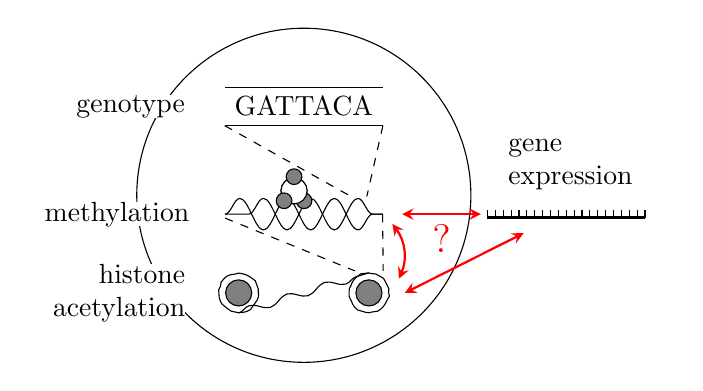
\begin{tikzpicture}
    \node (g) {GATTACA};
    \draw (g.north west) -- (g.north east);
    \draw (g.south west) -- (g.south east);

    \node [below left= of g.south] (m1) {};
    \node [below right= of g.south] (m2) {};
    \draw [decorate, decoration={snake, segment length=6mm, amplitude=2mm}] (m1) -- (m2);
    \draw [decorate, decoration={snake, segment length=6mm, amplitude=2mm, pre length=3mm}] (m1) -- (m2);
    \node [right=1cm of m1.north, anchor=south, circle, draw, fill=white] (me) { };
    \node [below right=-0.1 of me.south east, anchor=north west, circle, draw, fill=gray, inner sep=2pt] { };
    \node [right=1cm of m1.north, anchor=south, circle, draw, fill=white] (me) { };
    \node [below left=-0.1 of me.south west, anchor=north east, circle, draw, fill=gray, inner sep=2pt] { };
    \node [above=-0.1 of me.north, anchor=south, circle, draw, fill=gray, inner sep=2pt] { };

    \node [below= of m1.east, anchor=west, circle, draw, fill=gray] (a1) { };
    \node [below= of m2.west, anchor=east, circle, draw, fill=gray] (a2) { };
    \node [above=0 of a1.center, anchor=center, circle, draw, decorate,
           decoration={random steps, amplitude=0.1mm, segment length=0.5mm}, 
           inner sep=5pt] (a1out) { };
    \node [above=0 of a2.center, anchor=center, circle, draw, decorate,
           decoration={random steps, amplitude=0.1mm, segment length=0.5mm}, 
           inner sep=5pt] (a2out) { };
    \draw [decorate, decoration={snake, amplitude=0.5mm, segment length=5mm}]
          (a1out.south) -- (a2out.north);

    \draw [dashed] (g.south west) -- ($(m2.north west) + (-4mm, 1mm)$);
    \draw [dashed] (g.south east) -- ($(m2.north west) + (-2mm, 1mm)$);

    \draw [dashed] (m1) -- ($(a2out.north west) + (0mm, 1mm)$);
    \draw [dashed] (m2.west) -- ($(a2out.north east) + (0mm, 1mm)$);

    \node [circle, draw, above=of g.center, anchor=north, inner sep=1.5cm] { };

    \node [right=1cm of m2, inner sep=1pt] (e1) { };
    \node [right=2cm of e1, inner sep=1pt] (e2) { };
    \draw [decorate, decoration={ticks, amplitude=0.5mm, segment length=1mm}] (e1) -- (e2);
    \draw [thick] (e1.south east) -- (e2.south west);

    \uncover<3-> {
    \draw [<->, >=stealth, thick, color=red] (e1) -- node [auto, color=red] {\Large{?}} (m2);
    \draw [<->, >=stealth, thick, color=red] ($(e1.south) + (5mm, -2mm)$) -- 
    ($(a2out.east) + (2mm, 0mm)$);
    \path [bend left, draw, <->, >=stealth, thick, color=red] (m2.south) to 
    ($(a2out.north east) + (2mm, 0)$);
    }

    \node [above right=2mm of e1, text width=2cm] {gene \\ expression};
    \node [left=2mm of m1, fill=white, inner sep=0pt, align=right] {methylation};
    \node [left=5mm of a1, fill=white, inner sep=0pt, text width=2cm,
    align=right] {histone \\ acetylation};
    \node [left=5mm of g.west, fill=white, inner sep=0pt, align=right] {genotype};
\end{tikzpicture}

    \end{center}
        \uncover<3->{
        \item \textbf{how do these data fit together?}
        }
    \end{itemize}
\end{frame}

\begin{frame}{The data}
    \begin{columns}
        \begin{column}{0.35\textwidth}
            \begin{itemize}
                \item large cohort designed to study cognitive decline and
                    Alzheimer's disease
                \uncover<2->{
                \item genotype, gene expression, DNA methylation, and histone
                    acetylation (CHiP-seq) data 
                }
                \uncover<3->{
                \item 392 individuals with all four data types were used for
                    this analysis
                }
            \end{itemize}
        \end{column}
        \begin{column}{0.7\textwidth}
            % Created by tikzDevice version 0.7.0 on 2015-03-24 22:21:56
% !TEX encoding = UTF-8 Unicode
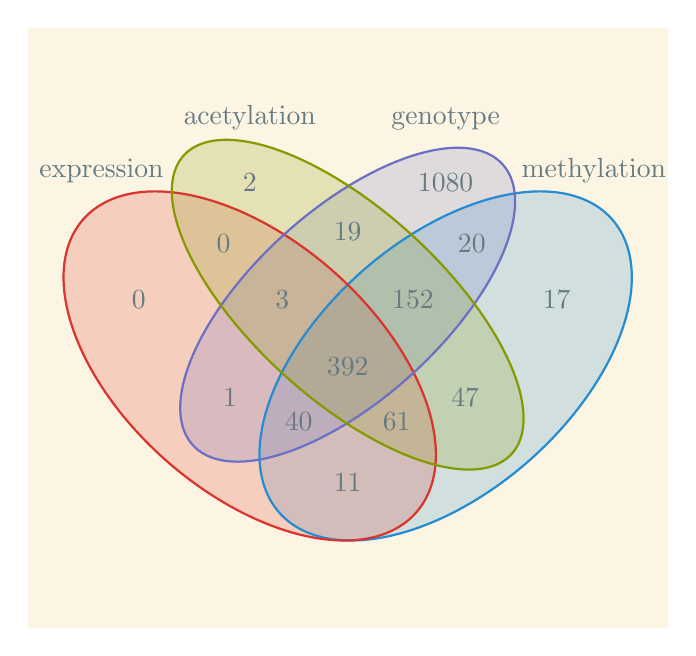
\begin{tikzpicture}[x=1pt,y=1pt]
\definecolor[named]{fillColor}{rgb}{0.99,0.96,0.89}
\path[use as bounding box,fill=fillColor] (0,0) rectangle (231.26,216.81);
\begin{scope}
\path[clip] (  0.00,  0.00) rectangle (231.26,216.81);
\definecolor[named]{fillColor}{rgb}{0.15,0.55,0.82}

\path[fill=fillColor,fill opacity=0.20] (209.44,149.34) --
	(209.37,149.41) --
	(209.30,149.47) --
	(209.23,149.54) --
	(209.16,149.60) --
	(209.09,149.66) --
	(209.02,149.73) --
	(208.95,149.79) --
	(208.88,149.86) --
	(208.80,149.92) --
	(208.73,149.98) --
	(208.66,150.05) --
	(208.59,150.11) --
	(208.51,150.17) --
	(208.44,150.23) --
	(208.37,150.30) --
	(208.29,150.36) --
	(208.22,150.42) --
	(208.14,150.48) --
	(208.07,150.54) --
	(207.99,150.60) --
	(207.92,150.66) --
	(207.84,150.72) --
	(207.77,150.78) --
	(207.69,150.84) --
	(207.62,150.90) --
	(207.54,150.96) --
	(207.46,151.02) --
	(207.39,151.08) --
	(207.31,151.14) --
	(207.23,151.20) --
	(207.15,151.26) --
	(207.08,151.31) --
	(207.00,151.37) --
	(206.92,151.43) --
	(206.84,151.48) --
	(206.76,151.54) --
	(206.68,151.60) --
	(206.60,151.65) --
	(206.53,151.71) --
	(206.45,151.77) --
	(206.37,151.82) --
	(206.29,151.88) --
	(206.20,151.93) --
	(206.12,151.99) --
	(206.04,152.04) --
	(205.96,152.10) --
	(205.88,152.15) --
	(205.80,152.20) --
	(205.72,152.26) --
	(205.63,152.31) --
	(205.55,152.36) --
	(205.47,152.42) --
	(205.39,152.47) --
	(205.30,152.52) --
	(205.22,152.57) --
	(205.14,152.63) --
	(205.05,152.68) --
	(204.97,152.73) --
	(204.88,152.78) --
	(204.80,152.83) --
	(204.71,152.88) --
	(204.63,152.93) --
	(204.54,152.98) --
	(204.46,153.03) --
	(204.37,153.08) --
	(204.29,153.13) --
	(204.20,153.18) --
	(204.11,153.23) --
	(204.03,153.28) --
	(203.94,153.32) --
	(203.85,153.37) --
	(203.77,153.42) --
	(203.68,153.47) --
	(203.59,153.51) --
	(203.50,153.56) --
	(203.41,153.61) --
	(203.33,153.65) --
	(203.24,153.70) --
	(203.15,153.75) --
	(203.06,153.79) --
	(202.97,153.84) --
	(202.88,153.88) --
	(202.79,153.93) --
	(202.70,153.97) --
	(202.61,154.02) --
	(202.52,154.06) --
	(202.43,154.10) --
	(202.34,154.15) --
	(202.25,154.19) --
	(202.15,154.23) --
	(202.06,154.28) --
	(201.97,154.32) --
	(201.88,154.36) --
	(201.79,154.40) --
	(201.69,154.44) --
	(201.60,154.49) --
	(201.51,154.53) --
	(201.41,154.57) --
	(201.32,154.61) --
	(201.23,154.65) --
	(201.13,154.69) --
	(201.04,154.73) --
	(200.95,154.77) --
	(200.85,154.81) --
	(200.76,154.85) --
	(200.66,154.89) --
	(200.57,154.92) --
	(200.47,154.96) --
	(200.37,155.00) --
	(200.28,155.04) --
	(200.18,155.08) --
	(200.09,155.11) --
	(199.99,155.15) --
	(199.89,155.19) --
	(199.80,155.22) --
	(199.70,155.26) --
	(199.60,155.30) --
	(199.50,155.33) --
	(199.41,155.37) --
	(199.31,155.40) --
	(199.21,155.44) --
	(199.11,155.47) --
	(199.01,155.51) --
	(198.91,155.54) --
	(198.81,155.57) --
	(198.72,155.61) --
	(198.62,155.64) --
	(198.52,155.67) --
	(198.42,155.71) --
	(198.32,155.74) --
	(198.22,155.77) --
	(198.12,155.80) --
	(198.01,155.83) --
	(197.91,155.86) --
	(197.81,155.90) --
	(197.71,155.93) --
	(197.61,155.96) --
	(197.51,155.99) --
	(197.41,156.02) --
	(197.30,156.05) --
	(197.20,156.08) --
	(197.10,156.11) --
	(197.00,156.13) --
	(196.89,156.16) --
	(196.79,156.19) --
	(196.69,156.22) --
	(196.58,156.25) --
	(196.48,156.28) --
	(196.37,156.30) --
	(196.27,156.33) --
	(196.17,156.36) --
	(196.06,156.38) --
	(195.96,156.41) --
	(195.85,156.43) --
	(195.75,156.46) --
	(195.64,156.49) --
	(195.54,156.51) --
	(195.43,156.54) --
	(195.32,156.56) --
	(195.22,156.58) --
	(195.11,156.61) --
	(195.00,156.63) --
	(194.90,156.66) --
	(194.79,156.68) --
	(194.68,156.70) --
	(194.58,156.72) --
	(194.47,156.75) --
	(194.36,156.77) --
	(194.25,156.79) --
	(194.15,156.81) --
	(194.04,156.83) --
	(193.93,156.86) --
	(193.82,156.88) --
	(193.71,156.90) --
	(193.60,156.92) --
	(193.49,156.94) --
	(193.38,156.96) --
	(193.27,156.98) --
	(193.16,156.99) --
	(193.05,157.01) --
	(192.94,157.03) --
	(192.83,157.05) --
	(192.72,157.07) --
	(192.61,157.09) --
	(192.50,157.10) --
	(192.39,157.12) --
	(192.28,157.14) --
	(192.17,157.15) --
	(192.06,157.17) --
	(191.95,157.19) --
	(191.83,157.20) --
	(191.72,157.22) --
	(191.61,157.23) --
	(191.50,157.25) --
	(191.38,157.26) --
	(191.27,157.28) --
	(191.16,157.29) --
	(191.04,157.31) --
	(190.93,157.32) --
	(190.82,157.33) --
	(190.70,157.35) --
	(190.59,157.36) --
	(190.48,157.37) --
	(190.36,157.38) --
	(190.25,157.40) --
	(190.13,157.41) --
	(190.02,157.42) --
	(189.90,157.43) --
	(189.79,157.44) --
	(189.67,157.45) --
	(189.56,157.46) --
	(189.44,157.47) --
	(189.33,157.48) --
	(189.21,157.49) --
	(189.09,157.50) --
	(188.98,157.51) --
	(188.86,157.52) --
	(188.75,157.53) --
	(188.63,157.53) --
	(188.51,157.54) --
	(188.39,157.55) --
	(188.28,157.56) --
	(188.16,157.56) --
	(188.04,157.57) --
	(187.92,157.58) --
	(187.81,157.58) --
	(187.69,157.59) --
	(187.57,157.60) --
	(187.45,157.60) --
	(187.33,157.61) --
	(187.21,157.61) --
	(187.10,157.62) --
	(186.98,157.62) --
	(186.86,157.62) --
	(186.74,157.63) --
	(186.62,157.63) --
	(186.50,157.63) --
	(186.38,157.64) --
	(186.26,157.64) --
	(186.14,157.64) --
	(186.02,157.64) --
	(185.90,157.65) --
	(185.78,157.65) --
	(185.66,157.65) --
	(185.54,157.65) --
	(185.42,157.65) --
	(185.29,157.65) --
	(185.17,157.65) --
	(185.05,157.65) --
	(184.93,157.65) --
	(184.81,157.65) --
	(184.69,157.65) --
	(184.56,157.65) --
	(184.44,157.64) --
	(184.32,157.64) --
	(184.20,157.64) --
	(184.07,157.64) --
	(183.95,157.64) --
	(183.83,157.63) --
	(183.71,157.63) --
	(183.58,157.63) --
	(183.46,157.62) --
	(183.33,157.62) --
	(183.21,157.61) --
	(183.09,157.61) --
	(182.96,157.60) --
	(182.84,157.60) --
	(182.72,157.59) --
	(182.59,157.59) --
	(182.47,157.58) --
	(182.34,157.58) --
	(182.22,157.57) --
	(182.09,157.56) --
	(181.97,157.56) --
	(181.84,157.55) --
	(181.72,157.54) --
	(181.59,157.53) --
	(181.47,157.52) --
	(181.34,157.52) --
	(181.21,157.51) --
	(181.09,157.50) --
	(180.96,157.49) --
	(180.84,157.48) --
	(180.71,157.47) --
	(180.58,157.46) --
	(180.46,157.45) --
	(180.33,157.44) --
	(180.20,157.43) --
	(180.08,157.42) --
	(179.95,157.40) --
	(179.82,157.39) --
	(179.69,157.38) --
	(179.57,157.37) --
	(179.44,157.36) --
	(179.31,157.34) --
	(179.18,157.33) --
	(179.05,157.32) --
	(178.93,157.30) --
	(178.80,157.29) --
	(178.67,157.27) --
	(178.54,157.26) --
	(178.41,157.25) --
	(178.28,157.23) --
	(178.15,157.21) --
	(178.03,157.20) --
	(177.90,157.18) --
	(177.77,157.17) --
	(177.64,157.15) --
	(177.51,157.13) --
	(177.38,157.12) --
	(177.25,157.10) --
	(177.12,157.08) --
	(176.99,157.06) --
	(176.86,157.05) --
	(176.73,157.03) --
	(176.60,157.01) --
	(176.47,156.99) --
	(176.34,156.97) --
	(176.21,156.95) --
	(176.08,156.93) --
	(175.95,156.91) --
	(175.82,156.89) --
	(175.68,156.87) --
	(175.55,156.85) --
	(175.42,156.83) --
	(175.29,156.81) --
	(175.16,156.79) --
	(175.03,156.76) --
	(174.90,156.74) --
	(174.76,156.72) --
	(174.63,156.70) --
	(174.50,156.67) --
	(174.37,156.65) --
	(174.24,156.63) --
	(174.10,156.60) --
	(173.97,156.58) --
	(173.84,156.55) --
	(173.71,156.53) --
	(173.57,156.50) --
	(173.44,156.48) --
	(173.31,156.45) --
	(173.17,156.43) --
	(173.04,156.40) --
	(172.91,156.38) --
	(172.77,156.35) --
	(172.64,156.32) --
	(172.51,156.30) --
	(172.37,156.27) --
	(172.24,156.24) --
	(172.11,156.21) --
	(171.97,156.18) --
	(171.84,156.16) --
	(171.71,156.13) --
	(171.57,156.10) --
	(171.44,156.07) --
	(171.30,156.04) --
	(171.17,156.01) --
	(171.03,155.98) --
	(170.90,155.95) --
	(170.76,155.92) --
	(170.63,155.89) --
	(170.49,155.86) --
	(170.36,155.83) --
	(170.22,155.79) --
	(170.09,155.76) --
	(169.95,155.73) --
	(169.82,155.70) --
	(169.68,155.66) --
	(169.55,155.63) --
	(169.41,155.60) --
	(169.28,155.56) --
	(169.14,155.53) --
	(169.01,155.50) --
	(168.87,155.46) --
	(168.73,155.43) --
	(168.60,155.39) --
	(168.46,155.36) --
	(168.33,155.32) --
	(168.19,155.29) --
	(168.05,155.25) --
	(167.92,155.21) --
	(167.78,155.18) --
	(167.64,155.14) --
	(167.51,155.10) --
	(167.37,155.07) --
	(167.23,155.03) --
	(167.10,154.99) --
	(166.96,154.95) --
	(166.82,154.92) --
	(166.69,154.88) --
	(166.55,154.84) --
	(166.41,154.80) --
	(166.28,154.76) --
	(166.14,154.72) --
	(166.00,154.68) --
	(165.86,154.64) --
	(165.73,154.60) --
	(165.59,154.56) --
	(165.45,154.52) --
	(165.31,154.48) --
	(165.18,154.43) --
	(165.04,154.39) --
	(164.90,154.35) --
	(164.76,154.31) --
	(164.62,154.27) --
	(164.49,154.22) --
	(164.35,154.18) --
	(164.21,154.14) --
	(164.07,154.09) --
	(163.93,154.05) --
	(163.80,154.00) --
	(163.66,153.96) --
	(163.52,153.92) --
	(163.38,153.87) --
	(163.24,153.83) --
	(163.10,153.78) --
	(162.96,153.73) --
	(162.83,153.69) --
	(162.69,153.64) --
	(162.55,153.60) --
	(162.41,153.55) --
	(162.27,153.50) --
	(162.13,153.45) --
	(161.99,153.41) --
	(161.85,153.36) --
	(161.71,153.31) --
	(161.58,153.26) --
	(161.44,153.21) --
	(161.30,153.17) --
	(161.16,153.12) --
	(161.02,153.07) --
	(160.88,153.02) --
	(160.74,152.97) --
	(160.60,152.92) --
	(160.46,152.87) --
	(160.32,152.82) --
	(160.18,152.77) --
	(160.04,152.72) --
	(159.90,152.66) --
	(159.76,152.61) --
	(159.62,152.56) --
	(159.48,152.51) --
	(159.34,152.46) --
	(159.20,152.40) --
	(159.06,152.35) --
	(158.92,152.30) --
	(158.78,152.24) --
	(158.64,152.19) --
	(158.50,152.14) --
	(158.36,152.08) --
	(158.22,152.03) --
	(158.08,151.97) --
	(157.94,151.92) --
	(157.80,151.86) --
	(157.66,151.81) --
	(157.52,151.75) --
	(157.38,151.70) --
	(157.24,151.64) --
	(157.10,151.58) --
	(156.96,151.53) --
	(156.82,151.47) --
	(156.68,151.41) --
	(156.54,151.36) --
	(156.40,151.30) --
	(156.26,151.24) --
	(156.12,151.18) --
	(155.98,151.12) --
	(155.84,151.07) --
	(155.70,151.01) --
	(155.56,150.95) --
	(155.42,150.89) --
	(155.28,150.83) --
	(155.13,150.77) --
	(154.99,150.71) --
	(154.85,150.65) --
	(154.71,150.59) --
	(154.57,150.53) --
	(154.43,150.47) --
	(154.29,150.40) --
	(154.15,150.34) --
	(154.01,150.28) --
	(153.87,150.22) --
	(153.73,150.16) --
	(153.59,150.09) --
	(153.45,150.03) --
	(153.31,149.97) --
	(153.16,149.90) --
	(153.02,149.84) --
	(152.88,149.78) --
	(152.74,149.71) --
	(152.60,149.65) --
	(152.46,149.58) --
	(152.32,149.52) --
	(152.18,149.45) --
	(152.04,149.39) --
	(151.90,149.32) --
	(151.76,149.26) --
	(151.61,149.19) --
	(151.47,149.13) --
	(151.33,149.06) --
	(151.19,148.99) --
	(151.05,148.93) --
	(150.91,148.86) --
	(150.77,148.79) --
	(150.63,148.72) --
	(150.49,148.66) --
	(150.35,148.59) --
	(150.21,148.52) --
	(150.07,148.45) --
	(149.92,148.38) --
	(149.78,148.31) --
	(149.64,148.24) --
	(149.50,148.17) --
	(149.36,148.10) --
	(149.22,148.03) --
	(149.08,147.96) --
	(148.94,147.89) --
	(148.80,147.82) --
	(148.66,147.75) --
	(148.52,147.68) --
	(148.38,147.61) --
	(148.23,147.54) --
	(148.09,147.47) --
	(147.95,147.39) --
	(147.81,147.32) --
	(147.67,147.25) --
	(147.53,147.18) --
	(147.39,147.10) --
	(147.25,147.03) --
	(147.11,146.96) --
	(146.97,146.88) --
	(146.83,146.81) --
	(146.69,146.73) --
	(146.55,146.66) --
	(146.41,146.59) --
	(146.26,146.51) --
	(146.12,146.44) --
	(145.98,146.36) --
	(145.84,146.29) --
	(145.70,146.21) --
	(145.56,146.13) --
	(145.42,146.06) --
	(145.28,145.98) --
	(145.14,145.90) --
	(145.00,145.83) --
	(144.86,145.75) --
	(144.72,145.67) --
	(144.58,145.60) --
	(144.44,145.52) --
	(144.30,145.44) --
	(144.16,145.36) --
	(144.02,145.28) --
	(143.88,145.20) --
	(143.74,145.13) --
	(143.60,145.05) --
	(143.46,144.97) --
	(143.32,144.89) --
	(143.18,144.81) --
	(143.04,144.73) --
	(142.90,144.65) --
	(142.76,144.57) --
	(142.62,144.49) --
	(142.48,144.41) --
	(142.34,144.32) --
	(142.20,144.24) --
	(142.06,144.16) --
	(141.92,144.08) --
	(141.78,144.00) --
	(141.64,143.92) --
	(141.50,143.83) --
	(141.36,143.75) --
	(141.22,143.67) --
	(141.08,143.58) --
	(140.95,143.50) --
	(140.81,143.42) --
	(140.67,143.33) --
	(140.53,143.25) --
	(140.39,143.17) --
	(140.25,143.08) --
	(140.11,143.00) --
	(139.97,142.91) --
	(139.83,142.83) --
	(139.69,142.74) --
	(139.55,142.66) --
	(139.42,142.57) --
	(139.28,142.49) --
	(139.14,142.40) --
	(139.00,142.31) --
	(138.86,142.23) --
	(138.72,142.14) --
	(138.58,142.05) --
	(138.45,141.97) --
	(138.31,141.88) --
	(138.17,141.79) --
	(138.03,141.70) --
	(137.89,141.62) --
	(137.75,141.53) --
	(137.62,141.44) --
	(137.48,141.35) --
	(137.34,141.26) --
	(137.20,141.17) --
	(137.06,141.08) --
	(136.93,140.99) --
	(136.79,140.91) --
	(136.65,140.82) --
	(136.51,140.73) --
	(136.38,140.64) --
	(136.24,140.54) --
	(136.10,140.45) --
	(135.96,140.36) --
	(135.83,140.27) --
	(135.69,140.18) --
	(135.55,140.09) --
	(135.41,140.00) --
	(135.28,139.91) --
	(135.14,139.81) --
	(135.00,139.72) --
	(134.87,139.63) --
	(134.73,139.54) --
	(134.59,139.45) --
	(134.46,139.35) --
	(134.32,139.26) --
	(134.18,139.17) --
	(134.05,139.07) --
	(133.91,138.98) --
	(133.78,138.88) --
	(133.64,138.79) --
	(133.50,138.70) --
	(133.37,138.60) --
	(133.23,138.51) --
	(133.10,138.41) --
	(132.96,138.32) --
	(132.82,138.22) --
	(132.69,138.13) --
	(132.55,138.03) --
	(132.42,137.93) --
	(132.28,137.84) --
	(132.15,137.74) --
	(132.01,137.65) --
	(131.88,137.55) --
	(131.74,137.45) --
	(131.61,137.36) --
	(131.47,137.26) --
	(131.34,137.16) --
	(131.20,137.06) --
	(131.07,136.97) --
	(130.93,136.87) --
	(130.80,136.77) --
	(130.66,136.67) --
	(130.53,136.57) --
	(130.40,136.47) --
	(130.26,136.38) --
	(130.13,136.28) --
	(129.99,136.18) --
	(129.86,136.08) --
	(129.73,135.98) --
	(129.59,135.88) --
	(129.46,135.78) --
	(129.33,135.68) --
	(129.19,135.58) --
	(129.06,135.48) --
	(128.93,135.38) --
	(128.79,135.28) --
	(128.66,135.18) --
	(128.53,135.07) --
	(128.39,134.97) --
	(128.26,134.87) --
	(128.13,134.77) --
	(128.00,134.67) --
	(127.86,134.57) --
	(127.73,134.46) --
	(127.60,134.36) --
	(127.47,134.26) --
	(127.34,134.16) --
	(127.20,134.05) --
	(127.07,133.95) --
	(126.94,133.85) --
	(126.81,133.74) --
	(126.68,133.64) --
	(126.55,133.54) --
	(126.42,133.43) --
	(126.29,133.33) --
	(126.15,133.22) --
	(126.02,133.12) --
	(125.89,133.01) --
	(125.76,132.91) --
	(125.63,132.80) --
	(125.50,132.70) --
	(125.37,132.59) --
	(125.24,132.49) --
	(125.11,132.38) --
	(124.98,132.28) --
	(124.85,132.17) --
	(124.72,132.06) --
	(124.59,131.96) --
	(124.46,131.85) --
	(124.33,131.75) --
	(124.20,131.64) --
	(124.07,131.53) --
	(123.94,131.42) --
	(123.82,131.32) --
	(123.69,131.21) --
	(123.56,131.10) --
	(123.43,130.99) --
	(123.30,130.89) --
	(123.17,130.78) --
	(123.05,130.67) --
	(122.92,130.56) --
	(122.79,130.45) --
	(122.66,130.34) --
	(122.53,130.24) --
	(122.41,130.13) --
	(122.28,130.02) --
	(122.15,129.91) --
	(122.02,129.80) --
	(121.90,129.69) --
	(121.77,129.58) --
	(121.64,129.47) --
	(121.52,129.36) --
	(121.39,129.25) --
	(121.26,129.14) --
	(121.14,129.03) --
	(121.01,128.92) --
	(120.89,128.81) --
	(120.76,128.70) --
	(120.63,128.58) --
	(120.51,128.47) --
	(120.38,128.36) --
	(120.26,128.25) --
	(120.13,128.14) --
	(120.01,128.03) --
	(119.88,127.91) --
	(119.76,127.80) --
	(119.63,127.69) --
	(119.51,127.58) --
	(119.38,127.46) --
	(119.26,127.35) --
	(119.14,127.24) --
	(119.01,127.13) --
	(118.89,127.01) --
	(118.76,126.90) --
	(118.64,126.79) --
	(118.52,126.67) --
	(118.39,126.56) --
	(118.27,126.44) --
	(118.15,126.33) --
	(118.02,126.22) --
	(117.90,126.10) --
	(117.78,125.99) --
	(117.66,125.87) --
	(117.53,125.76) --
	(117.41,125.64) --
	(117.29,125.53) --
	(117.17,125.41) --
	(117.05,125.30) --
	(116.93,125.18) --
	(116.80,125.07) --
	(116.68,124.95) --
	(116.56,124.83) --
	(116.44,124.72) --
	(116.32,124.60) --
	(116.20,124.49) --
	(116.08,124.37) --
	(115.96,124.25) --
	(115.84,124.14) --
	(115.72,124.02) --
	(115.60,123.90) --
	(115.48,123.79) --
	(115.36,123.67) --
	(115.24,123.55) --
	(115.12,123.43) --
	(115.00,123.32) --
	(114.88,123.20) --
	(114.76,123.08) --
	(114.65,122.96) --
	(114.53,122.85) --
	(114.41,122.73) --
	(114.29,122.61) --
	(114.17,122.49) --
	(114.05,122.37) --
	(113.94,122.25) --
	(113.82,122.13) --
	(113.70,122.02) --
	(113.59,121.90) --
	(113.47,121.78) --
	(113.35,121.66) --
	(113.24,121.54) --
	(113.12,121.42) --
	(113.00,121.30) --
	(112.89,121.18) --
	(112.77,121.06) --
	(112.65,120.94) --
	(112.54,120.82) --
	(112.42,120.70) --
	(112.31,120.58) --
	(112.19,120.46) --
	(112.08,120.34) --
	(111.96,120.22) --
	(111.85,120.10) --
	(111.73,119.98) --
	(111.62,119.86) --
	(111.51,119.73) --
	(111.39,119.61) --
	(111.28,119.49) --
	(111.16,119.37) --
	(111.05,119.25) --
	(110.94,119.13) --
	(110.82,119.01) --
	(110.71,118.88) --
	(110.60,118.76) --
	(110.49,118.64) --
	(110.37,118.52) --
	(110.26,118.40) --
	(110.15,118.27) --
	(110.04,118.15) --
	(109.93,118.03) --
	(109.82,117.91) --
	(109.70,117.78) --
	(109.59,117.66) --
	(109.48,117.54) --
	(109.37,117.41) --
	(109.26,117.29) --
	(109.15,117.17) --
	(109.04,117.04) --
	(108.93,116.92) --
	(108.82,116.80) --
	(108.71,116.67) --
	(108.60,116.55) --
	(108.49,116.43) --
	(108.38,116.30) --
	(108.27,116.18) --
	(108.17,116.05) --
	(108.06,115.93) --
	(107.95,115.80) --
	(107.84,115.68) --
	(107.73,115.56) --
	(107.63,115.43) --
	(107.52,115.31) --
	(107.41,115.18) --
	(107.30,115.06) --
	(107.20,114.93) --
	(107.09,114.81) --
	(106.98,114.68) --
	(106.88,114.56) --
	(106.77,114.43) --
	(106.66,114.31) --
	(106.56,114.18) --
	(106.45,114.05) --
	(106.35,113.93) --
	(106.24,113.80) --
	(106.14,113.68) --
	(106.03,113.55) --
	(105.93,113.43) --
	(105.82,113.30) --
	(105.72,113.17) --
	(105.61,113.05) --
	(105.51,112.92) --
	(105.41,112.79) --
	(105.30,112.67) --
	(105.20,112.54) --
	(105.10,112.41) --
	(104.99,112.29) --
	(104.89,112.16) --
	(104.79,112.03) --
	(104.69,111.91) --
	(104.59,111.78) --
	(104.48,111.65) --
	(104.38,111.53) --
	(104.28,111.40) --
	(104.18,111.27) --
	(104.08,111.14) --
	(103.98,111.02) --
	(103.88,110.89) --
	(103.78,110.76) --
	(103.68,110.63) --
	(103.58,110.51) --
	(103.48,110.38) --
	(103.38,110.25) --
	(103.28,110.12) --
	(103.18,109.99) --
	(103.08,109.87) --
	(102.98,109.74) --
	(102.88,109.61) --
	(102.78,109.48) --
	(102.69,109.35) --
	(102.59,109.22) --
	(102.49,109.10) --
	(102.39,108.97) --
	(102.30,108.84) --
	(102.20,108.71) --
	(102.10,108.58) --
	(102.01,108.45) --
	(101.91,108.32) --
	(101.81,108.19) --
	(101.72,108.06) --
	(101.62,107.94) --
	(101.53,107.81) --
	(101.43,107.68) --
	(101.34,107.55) --
	(101.24,107.42) --
	(101.15,107.29) --
	(101.05,107.16) --
	(100.96,107.03) --
	(100.86,106.90) --
	(100.77,106.77) --
	(100.68,106.64) --
	(100.58,106.51) --
	(100.49,106.38) --
	(100.40,106.25) --
	(100.30,106.12) --
	(100.21,105.99) --
	(100.12,105.86) --
	(100.03,105.73) --
	( 99.94,105.60) --
	( 99.84,105.47) --
	( 99.75,105.34) --
	( 99.66,105.21) --
	( 99.57,105.08) --
	( 99.48,104.95) --
	( 99.39,104.82) --
	( 99.30,104.69) --
	( 99.21,104.56) --
	( 99.12,104.43) --
	( 99.03,104.30) --
	( 98.94,104.17) --
	( 98.85,104.04) --
	( 98.76,103.91) --
	( 98.67,103.78) --
	( 98.59,103.65) --
	( 98.50,103.52) --
	( 98.41,103.39) --
	( 98.32,103.25) --
	( 98.24,103.12) --
	( 98.15,102.99) --
	( 98.06,102.86) --
	( 97.97,102.73) --
	( 97.89,102.60) --
	( 97.80,102.47) --
	( 97.72,102.34) --
	( 97.63,102.21) --
	( 97.54,102.08) --
	( 97.46,101.94) --
	( 97.37,101.81) --
	( 97.29,101.68) --
	( 97.20,101.55) --
	( 97.12,101.42) --
	( 97.04,101.29) --
	( 96.95,101.16) --
	( 96.87,101.03) --
	( 96.78,100.89) --
	( 96.70,100.76) --
	( 96.62,100.63) --
	( 96.54,100.50) --
	( 96.45,100.37) --
	( 96.37,100.24) --
	( 96.29,100.11) --
	( 96.21, 99.97) --
	( 96.13, 99.84) --
	( 96.04, 99.71) --
	( 95.96, 99.58) --
	( 95.88, 99.45) --
	( 95.80, 99.32) --
	( 95.72, 99.18) --
	( 95.64, 99.05) --
	( 95.56, 98.92) --
	( 95.48, 98.79) --
	( 95.40, 98.66) --
	( 95.32, 98.52) --
	( 95.25, 98.39) --
	( 95.17, 98.26) --
	( 95.09, 98.13) --
	( 95.01, 98.00) --
	( 94.93, 97.87) --
	( 94.85, 97.73) --
	( 94.78, 97.60) --
	( 94.70, 97.47) --
	( 94.62, 97.34) --
	( 94.55, 97.21) --
	( 94.47, 97.07) --
	( 94.39, 96.94) --
	( 94.32, 96.81) --
	( 94.24, 96.68) --
	( 94.17, 96.55) --
	( 94.09, 96.41) --
	( 94.02, 96.28) --
	( 93.94, 96.15) --
	( 93.87, 96.02) --
	( 93.79, 95.89) --
	( 93.72, 95.75) --
	( 93.65, 95.62) --
	( 93.57, 95.49) --
	( 93.50, 95.36) --
	( 93.43, 95.22) --
	( 93.35, 95.09) --
	( 93.28, 94.96) --
	( 93.21, 94.83) --
	( 93.14, 94.70) --
	( 93.07, 94.56) --
	( 92.99, 94.43) --
	( 92.92, 94.30) --
	( 92.85, 94.17) --
	( 92.78, 94.04) --
	( 92.71, 93.90) --
	( 92.64, 93.77) --
	( 92.57, 93.64) --
	( 92.50, 93.51) --
	( 92.43, 93.38) --
	( 92.36, 93.24) --
	( 92.29, 93.11) --
	( 92.23, 92.98) --
	( 92.16, 92.85) --
	( 92.09, 92.72) --
	( 92.02, 92.58) --
	( 91.95, 92.45) --
	( 91.89, 92.32) --
	( 91.82, 92.19) --
	( 91.75, 92.06) --
	( 91.69, 91.92) --
	( 91.62, 91.79) --
	( 91.56, 91.66) --
	( 91.49, 91.53) --
	( 91.42, 91.40) --
	( 91.36, 91.26) --
	( 91.29, 91.13) --
	( 91.23, 91.00) --
	( 91.16, 90.87) --
	( 91.10, 90.74) --
	( 91.04, 90.60) --
	( 90.97, 90.47) --
	( 90.91, 90.34) --
	( 90.85, 90.21) --
	( 90.78, 90.08) --
	( 90.72, 89.95) --
	( 90.66, 89.81) --
	( 90.60, 89.68) --
	( 90.54, 89.55) --
	( 90.47, 89.42) --
	( 90.41, 89.29) --
	( 90.35, 89.16) --
	( 90.29, 89.02) --
	( 90.23, 88.89) --
	( 90.17, 88.76) --
	( 90.11, 88.63) --
	( 90.05, 88.50) --
	( 89.99, 88.37) --
	( 89.93, 88.23) --
	( 89.87, 88.10) --
	( 89.82, 87.97) --
	( 89.76, 87.84) --
	( 89.70, 87.71) --
	( 89.64, 87.58) --
	( 89.58, 87.45) --
	( 89.53, 87.32) --
	( 89.47, 87.18) --
	( 89.41, 87.05) --
	( 89.36, 86.92) --
	( 89.30, 86.79) --
	( 89.24, 86.66) --
	( 89.19, 86.53) --
	( 89.13, 86.40) --
	( 89.08, 86.27) --
	( 89.02, 86.14) --
	( 88.97, 86.01) --
	( 88.91, 85.87) --
	( 88.86, 85.74) --
	( 88.81, 85.61) --
	( 88.75, 85.48) --
	( 88.70, 85.35) --
	( 88.65, 85.22) --
	( 88.60, 85.09) --
	( 88.54, 84.96) --
	( 88.49, 84.83) --
	( 88.44, 84.70) --
	( 88.39, 84.57) --
	( 88.34, 84.44) --
	( 88.29, 84.31) --
	( 88.23, 84.18) --
	( 88.18, 84.05) --
	( 88.13, 83.92) --
	( 88.08, 83.79) --
	( 88.03, 83.66) --
	( 87.99, 83.53) --
	( 87.94, 83.40) --
	( 87.89, 83.27) --
	( 87.84, 83.14) --
	( 87.79, 83.01) --
	( 87.74, 82.88) --
	( 87.70, 82.75) --
	( 87.65, 82.62) --
	( 87.60, 82.49) --
	( 87.55, 82.36) --
	( 87.51, 82.23) --
	( 87.46, 82.10) --
	( 87.42, 81.97) --
	( 87.37, 81.84) --
	( 87.32, 81.71) --
	( 87.28, 81.58) --
	( 87.23, 81.45) --
	( 87.19, 81.32) --
	( 87.15, 81.19) --
	( 87.10, 81.06) --
	( 87.06, 80.94) --
	( 87.01, 80.81) --
	( 86.97, 80.68) --
	( 86.93, 80.55) --
	( 86.89, 80.42) --
	( 86.84, 80.29) --
	( 86.80, 80.16) --
	( 86.76, 80.03) --
	( 86.72, 79.91) --
	( 86.68, 79.78) --
	( 86.64, 79.65) --
	( 86.60, 79.52) --
	( 86.56, 79.39) --
	( 86.52, 79.26) --
	( 86.48, 79.14) --
	( 86.44, 79.01) --
	( 86.40, 78.88) --
	( 86.36, 78.75) --
	( 86.32, 78.62) --
	( 86.28, 78.50) --
	( 86.24, 78.37) --
	( 86.21, 78.24) --
	( 86.17, 78.11) --
	( 86.13, 77.99) --
	( 86.09, 77.86) --
	( 86.06, 77.73) --
	( 86.02, 77.60) --
	( 85.98, 77.48) --
	( 85.95, 77.35) --
	( 85.91, 77.22) --
	( 85.88, 77.10) --
	( 85.84, 76.97) --
	( 85.81, 76.84) --
	( 85.77, 76.72) --
	( 85.74, 76.59) --
	( 85.71, 76.46) --
	( 85.67, 76.34) --
	( 85.64, 76.21) --
	( 85.61, 76.08) --
	( 85.57, 75.96) --
	( 85.54, 75.83) --
	( 85.51, 75.71) --
	( 85.48, 75.58) --
	( 85.45, 75.45) --
	( 85.42, 75.33) --
	( 85.38, 75.20) --
	( 85.35, 75.08) --
	( 85.32, 74.95) --
	( 85.29, 74.82) --
	( 85.26, 74.70) --
	( 85.23, 74.57) --
	( 85.20, 74.45) --
	( 85.18, 74.32) --
	( 85.15, 74.20) --
	( 85.12, 74.07) --
	( 85.09, 73.95) --
	( 85.06, 73.82) --
	( 85.04, 73.70) --
	( 85.01, 73.57) --
	( 84.98, 73.45) --
	( 84.96, 73.33) --
	( 84.93, 73.20) --
	( 84.90, 73.08) --
	( 84.88, 72.95) --
	( 84.85, 72.83) --
	( 84.83, 72.71) --
	( 84.80, 72.58) --
	( 84.78, 72.46) --
	( 84.75, 72.33) --
	( 84.73, 72.21) --
	( 84.71, 72.09) --
	( 84.68, 71.96) --
	( 84.66, 71.84) --
	( 84.64, 71.72) --
	( 84.61, 71.59) --
	( 84.59, 71.47) --
	( 84.57, 71.35) --
	( 84.55, 71.23) --
	( 84.53, 71.10) --
	( 84.51, 70.98) --
	( 84.48, 70.86) --
	( 84.46, 70.74) --
	( 84.44, 70.61) --
	( 84.42, 70.49) --
	( 84.40, 70.37) --
	( 84.39, 70.25) --
	( 84.37, 70.13) --
	( 84.35, 70.00) --
	( 84.33, 69.88) --
	( 84.31, 69.76) --
	( 84.29, 69.64) --
	( 84.28, 69.52) --
	( 84.26, 69.40) --
	( 84.24, 69.28) --
	( 84.22, 69.15) --
	( 84.21, 69.03) --
	( 84.19, 68.91) --
	( 84.18, 68.79) --
	( 84.16, 68.67) --
	( 84.15, 68.55) --
	( 84.13, 68.43) --
	( 84.12, 68.31) --
	( 84.10, 68.19) --
	( 84.09, 68.07) --
	( 84.07, 67.95) --
	( 84.06, 67.83) --
	( 84.05, 67.71) --
	( 84.03, 67.59) --
	( 84.02, 67.47) --
	( 84.01, 67.35) --
	( 84.00, 67.24) --
	( 83.99, 67.12) --
	( 83.97, 67.00) --
	( 83.96, 66.88) --
	( 83.95, 66.76) --
	( 83.94, 66.64) --
	( 83.93, 66.52) --
	( 83.92, 66.41) --
	( 83.91, 66.29) --
	( 83.90, 66.17) --
	( 83.89, 66.05) --
	( 83.89, 65.93) --
	( 83.88, 65.82) --
	( 83.87, 65.70) --
	( 83.86, 65.58) --
	( 83.85, 65.46) --
	( 83.85, 65.35) --
	( 83.84, 65.23) --
	( 83.83, 65.11) --
	( 83.83, 65.00) --
	( 83.82, 64.88) --
	( 83.81, 64.76) --
	( 83.81, 64.65) --
	( 83.80, 64.53) --
	( 83.80, 64.41) --
	( 83.79, 64.30) --
	( 83.79, 64.18) --
	( 83.79, 64.07) --
	( 83.78, 63.95) --
	( 83.78, 63.84) --
	( 83.78, 63.72) --
	( 83.77, 63.61) --
	( 83.77, 63.49) --
	( 83.77, 63.38) --
	( 83.77, 63.26) --
	( 83.76, 63.15) --
	( 83.76, 63.03) --
	( 83.76, 62.92) --
	( 83.76, 62.80) --
	( 83.76, 62.69) --
	( 83.76, 62.58) --
	( 83.76, 62.46) --
	( 83.76, 62.35) --
	( 83.76, 62.24) --
	( 83.76, 62.12) --
	( 83.76, 62.01) --
	( 83.77, 61.90) --
	( 83.77, 61.78) --
	( 83.77, 61.67) --
	( 83.77, 61.56) --
	( 83.77, 61.44) --
	( 83.78, 61.33) --
	( 83.78, 61.22) --
	( 83.78, 61.11) --
	( 83.79, 61.00) --
	( 83.79, 60.88) --
	( 83.80, 60.77) --
	( 83.80, 60.66) --
	( 83.81, 60.55) --
	( 83.81, 60.44) --
	( 83.82, 60.33) --
	( 83.82, 60.22) --
	( 83.83, 60.11) --
	( 83.84, 60.00) --
	( 83.84, 59.89) --
	( 83.85, 59.78) --
	( 83.86, 59.67) --
	( 83.87, 59.56) --
	( 83.87, 59.45) --
	( 83.88, 59.34) --
	( 83.89, 59.23) --
	( 83.90, 59.12) --
	( 83.91, 59.01) --
	( 83.92, 58.90) --
	( 83.93, 58.79) --
	( 83.94, 58.68) --
	( 83.95, 58.57) --
	( 83.96, 58.46) --
	( 83.97, 58.36) --
	( 83.98, 58.25) --
	( 83.99, 58.14) --
	( 84.01, 58.03) --
	( 84.02, 57.93) --
	( 84.03, 57.82) --
	( 84.04, 57.71) --
	( 84.06, 57.60) --
	( 84.07, 57.50) --
	( 84.08, 57.39) --
	( 84.10, 57.28) --
	( 84.11, 57.18) --
	( 84.13, 57.07) --
	( 84.14, 56.96) --
	( 84.16, 56.86) --
	( 84.17, 56.75) --
	( 84.19, 56.65) --
	( 84.20, 56.54) --
	( 84.22, 56.44) --
	( 84.24, 56.33) --
	( 84.25, 56.23) --
	( 84.27, 56.12) --
	( 84.29, 56.02) --
	( 84.31, 55.91) --
	( 84.32, 55.81) --
	( 84.34, 55.70) --
	( 84.36, 55.60) --
	( 84.38, 55.50) --
	( 84.40, 55.39) --
	( 84.42, 55.29) --
	( 84.44, 55.19) --
	( 84.46, 55.08) --
	( 84.48, 54.98) --
	( 84.50, 54.88) --
	( 84.52, 54.78) --
	( 84.54, 54.67) --
	( 84.56, 54.57) --
	( 84.59, 54.47) --
	( 84.61, 54.37) --
	( 84.63, 54.26) --
	( 84.65, 54.16) --
	( 84.68, 54.06) --
	( 84.70, 53.96) --
	( 84.72, 53.86) --
	( 84.75, 53.76) --
	( 84.77, 53.66) --
	( 84.80, 53.56) --
	( 84.82, 53.46) --
	( 84.85, 53.36) --
	( 84.87, 53.26) --
	( 84.90, 53.16) --
	( 84.92, 53.06) --
	( 84.95, 52.96) --
	( 84.97, 52.86) --
	( 85.00, 52.76) --
	( 85.03, 52.66) --
	( 85.06, 52.56) --
	( 85.08, 52.47) --
	( 85.11, 52.37) --
	( 85.14, 52.27) --
	( 85.17, 52.17) --
	( 85.20, 52.07) --
	( 85.23, 51.98) --
	( 85.26, 51.88) --
	( 85.29, 51.78) --
	( 85.32, 51.68) --
	( 85.35, 51.59) --
	( 85.38, 51.49) --
	( 85.41, 51.40) --
	( 85.44, 51.30) --
	( 85.47, 51.20) --
	( 85.50, 51.11) --
	( 85.53, 51.01) --
	( 85.57, 50.92) --
	( 85.60, 50.82) --
	( 85.63, 50.73) --
	( 85.66, 50.63) --
	( 85.70, 50.54) --
	( 85.73, 50.44) --
	( 85.77, 50.35) --
	( 85.80, 50.25) --
	( 85.83, 50.16) --
	( 85.87, 50.07) --
	( 85.90, 49.97) --
	( 85.94, 49.88) --
	( 85.98, 49.79) --
	( 86.01, 49.69) --
	( 86.05, 49.60) --
	( 86.08, 49.51) --
	( 86.12, 49.42) --
	( 86.16, 49.32) --
	( 86.20, 49.23) --
	( 86.23, 49.14) --
	( 86.27, 49.05) --
	( 86.31, 48.96) --
	( 86.35, 48.87) --
	( 86.39, 48.78) --
	( 86.43, 48.68) --
	( 86.47, 48.59) --
	( 86.51, 48.50) --
	( 86.55, 48.41) --
	( 86.59, 48.32) --
	( 86.63, 48.23) --
	( 86.67, 48.14) --
	( 86.71, 48.06) --
	( 86.75, 47.97) --
	( 86.79, 47.88) --
	( 86.83, 47.79) --
	( 86.88, 47.70) --
	( 86.92, 47.61) --
	( 86.96, 47.52) --
	( 87.00, 47.44) --
	( 87.05, 47.35) --
	( 87.09, 47.26) --
	( 87.13, 47.17) --
	( 87.18, 47.09) --
	( 87.22, 47.00) --
	( 87.27, 46.91) --
	( 87.31, 46.83) --
	( 87.36, 46.74) --
	( 87.40, 46.66) --
	( 87.45, 46.57) --
	( 87.50, 46.48) --
	( 87.54, 46.40) --
	( 87.59, 46.31) --
	( 87.64, 46.23) --
	( 87.68, 46.14) --
	( 87.73, 46.06) --
	( 87.78, 45.98) --
	( 87.83, 45.89) --
	( 87.88, 45.81) --
	( 87.92, 45.72) --
	( 87.97, 45.64) --
	( 88.02, 45.56) --
	( 88.07, 45.47) --
	( 88.12, 45.39) --
	( 88.17, 45.31) --
	( 88.22, 45.23) --
	( 88.27, 45.14) --
	( 88.32, 45.06) --
	( 88.37, 44.98) --
	( 88.43, 44.90) --
	( 88.48, 44.82) --
	( 88.53, 44.74) --
	( 88.58, 44.66) --
	( 88.63, 44.58) --
	( 88.69, 44.49) --
	( 88.74, 44.41) --
	( 88.79, 44.33) --
	( 88.85, 44.26) --
	( 88.90, 44.18) --
	( 88.96, 44.10) --
	( 89.01, 44.02) --
	( 89.06, 43.94) --
	( 89.12, 43.86) --
	( 89.17, 43.78) --
	( 89.23, 43.70) --
	( 89.29, 43.63) --
	( 89.34, 43.55) --
	( 89.40, 43.47) --
	( 89.46, 43.39) --
	( 89.51, 43.32) --
	( 89.57, 43.24) --
	( 89.63, 43.16) --
	( 89.68, 43.09) --
	( 89.74, 43.01) --
	( 89.80, 42.93) --
	( 89.86, 42.86) --
	( 89.92, 42.78) --
	( 89.98, 42.71) --
	( 90.04, 42.63) --
	( 90.10, 42.56) --
	( 90.16, 42.48) --
	( 90.22, 42.41) --
	( 90.28, 42.33) --
	( 90.34, 42.26) --
	( 90.40, 42.19) --
	( 90.46, 42.11) --
	( 90.52, 42.04) --
	( 90.58, 41.97) --
	( 90.64, 41.89) --
	( 90.71, 41.82) --
	( 90.77, 41.75) --
	( 90.83, 41.68) --
	( 90.89, 41.61) --
	( 90.96, 41.53) --
	( 91.02, 41.46) --
	( 91.08, 41.39) --
	( 91.15, 41.32) --
	( 91.21, 41.25) --
	( 91.28, 41.18) --
	( 91.34, 41.11) --
	( 91.41, 41.04) --
	( 91.47, 40.97) --
	( 91.54, 40.90) --
	( 91.60, 40.83) --
	( 91.67, 40.76) --
	( 91.74, 40.69) --
	( 91.80, 40.63) --
	( 91.87, 40.56) --
	( 91.94, 40.49) --
	( 92.01, 40.42) --
	( 92.07, 40.35) --
	( 92.14, 40.29) --
	( 92.21, 40.22) --
	( 92.28, 40.15) --
	( 92.35, 40.09) --
	( 92.42, 40.02) --
	( 92.48, 39.95) --
	( 92.55, 39.89) --
	( 92.62, 39.82) --
	( 92.69, 39.76) --
	( 92.76, 39.69) --
	( 92.83, 39.63) --
	( 92.91, 39.56) --
	( 92.98, 39.50) --
	( 93.05, 39.43) --
	( 93.12, 39.37) --
	( 93.19, 39.31) --
	( 93.26, 39.24) --
	( 93.34, 39.18) --
	( 93.41, 39.12) --
	( 93.48, 39.05) --
	( 93.55, 38.99) --
	( 93.63, 38.93) --
	( 93.70, 38.87) --
	( 93.77, 38.80) --
	( 93.85, 38.74) --
	( 93.92, 38.68) --
	( 94.00, 38.62) --
	( 94.07, 38.56) --
	( 94.15, 38.50) --
	( 94.22, 38.44) --
	( 94.30, 38.38) --
	( 94.37, 38.32) --
	( 94.45, 38.26) --
	( 94.53, 38.20) --
	( 94.60, 38.14) --
	( 94.68, 38.08) --
	( 94.76, 38.02) --
	( 94.83, 37.97) --
	( 94.91, 37.91) --
	( 94.99, 37.85) --
	( 95.07, 37.79) --
	( 95.15, 37.73) --
	( 95.23, 37.68) --
	( 95.30, 37.62) --
	( 95.38, 37.56) --
	( 95.46, 37.51) --
	( 95.54, 37.45) --
	( 95.62, 37.40) --
	( 95.70, 37.34) --
	( 95.78, 37.28) --
	( 95.86, 37.23) --
	( 95.94, 37.17) --
	( 96.02, 37.12) --
	( 96.11, 37.07) --
	( 96.19, 37.01) --
	( 96.27, 36.96) --
	( 96.35, 36.90) --
	( 96.43, 36.85) --
	( 96.52, 36.80) --
	( 96.60, 36.75) --
	( 96.68, 36.69) --
	( 96.76, 36.64) --
	( 96.85, 36.59) --
	( 96.93, 36.54) --
	( 97.01, 36.49) --
	( 97.10, 36.43) --
	( 97.18, 36.38) --
	( 97.27, 36.33) --
	( 97.35, 36.28) --
	( 97.44, 36.23) --
	( 97.52, 36.18) --
	( 97.61, 36.13) --
	( 97.69, 36.08) --
	( 97.78, 36.03) --
	( 97.87, 35.98) --
	( 97.95, 35.93) --
	( 98.04, 35.89) --
	( 98.13, 35.84) --
	( 98.21, 35.79) --
	( 98.30, 35.74) --
	( 98.39, 35.70) --
	( 98.48, 35.65) --
	( 98.56, 35.60) --
	( 98.65, 35.55) --
	( 98.74, 35.51) --
	( 98.83, 35.46) --
	( 98.92, 35.42) --
	( 99.01, 35.37) --
	( 99.10, 35.33) --
	( 99.19, 35.28) --
	( 99.28, 35.24) --
	( 99.37, 35.19) --
	( 99.46, 35.15) --
	( 99.55, 35.10) --
	( 99.64, 35.06) --
	( 99.73, 35.01) --
	( 99.82, 34.97) --
	( 99.91, 34.93) --
	(100.00, 34.89) --
	(100.10, 34.84) --
	(100.19, 34.80) --
	(100.28, 34.76) --
	(100.37, 34.72) --
	(100.47, 34.68) --
	(100.56, 34.63) --
	(100.65, 34.59) --
	(100.75, 34.55) --
	(100.84, 34.51) --
	(100.93, 34.47) --
	(101.03, 34.43) --
	(101.12, 34.39) --
	(101.22, 34.35) --
	(101.31, 34.31) --
	(101.41, 34.28) --
	(101.50, 34.24) --
	(101.60, 34.20) --
	(101.69, 34.16) --
	(101.79, 34.12) --
	(101.88, 34.09) --
	(101.98, 34.05) --
	(102.08, 34.01) --
	(102.17, 33.98) --
	(102.27, 33.94) --
	(102.37, 33.90) --
	(102.47, 33.87) --
	(102.56, 33.83) --
	(102.66, 33.80) --
	(102.76, 33.76) --
	(102.86, 33.73) --
	(102.96, 33.69) --
	(103.05, 33.66) --
	(103.15, 33.62) --
	(103.25, 33.59) --
	(103.35, 33.56) --
	(103.45, 33.52) --
	(103.55, 33.49) --
	(103.65, 33.46) --
	(103.75, 33.42) --
	(103.85, 33.39) --
	(103.95, 33.36) --
	(104.05, 33.33) --
	(104.15, 33.30) --
	(104.26, 33.27) --
	(104.36, 33.24) --
	(104.46, 33.21) --
	(104.56, 33.17) --
	(104.66, 33.14) --
	(104.76, 33.12) --
	(104.87, 33.09) --
	(104.97, 33.06) --
	(105.07, 33.03) --
	(105.17, 33.00) --
	(105.28, 32.97) --
	(105.38, 32.94) --
	(105.48, 32.91) --
	(105.59, 32.89) --
	(105.69, 32.86) --
	(105.80, 32.83) --
	(105.90, 32.81) --
	(106.01, 32.78) --
	(106.11, 32.75) --
	(106.22, 32.73) --
	(106.32, 32.70) --
	(106.43, 32.68) --
	(106.53, 32.65) --
	(106.64, 32.63) --
	(106.74, 32.60) --
	(106.85, 32.58) --
	(106.96, 32.55) --
	(107.06, 32.53) --
	(107.17, 32.51) --
	(107.28, 32.48) --
	(107.38, 32.46) --
	(107.49, 32.44) --
	(107.60, 32.41) --
	(107.71, 32.39) --
	(107.81, 32.37) --
	(107.92, 32.35) --
	(108.03, 32.33) --
	(108.14, 32.31) --
	(108.25, 32.29) --
	(108.36, 32.27) --
	(108.46, 32.25) --
	(108.57, 32.23) --
	(108.68, 32.21) --
	(108.79, 32.19) --
	(108.90, 32.17) --
	(109.01, 32.15) --
	(109.12, 32.13) --
	(109.23, 32.11) --
	(109.34, 32.09) --
	(109.45, 32.08) --
	(109.56, 32.06) --
	(109.68, 32.04) --
	(109.79, 32.02) --
	(109.90, 32.01) --
	(110.01, 31.99) --
	(110.12, 31.97) --
	(110.23, 31.96) --
	(110.35, 31.94) --
	(110.46, 31.93) --
	(110.57, 31.91) --
	(110.68, 31.90) --
	(110.80, 31.88) --
	(110.91, 31.87) --
	(111.02, 31.86) --
	(111.14, 31.84) --
	(111.25, 31.83) --
	(111.36, 31.82) --
	(111.48, 31.80) --
	(111.59, 31.79) --
	(111.71, 31.78) --
	(111.82, 31.77) --
	(111.93, 31.75) --
	(112.05, 31.74) --
	(112.16, 31.73) --
	(112.28, 31.72) --
	(112.39, 31.71) --
	(112.51, 31.70) --
	(112.63, 31.69) --
	(112.74, 31.68) --
	(112.86, 31.67) --
	(112.97, 31.66) --
	(113.09, 31.65) --
	(113.21, 31.64) --
	(113.32, 31.64) --
	(113.44, 31.63) --
	(113.56, 31.62) --
	(113.67, 31.61) --
	(113.79, 31.60) --
	(113.91, 31.60) --
	(114.03, 31.59) --
	(114.14, 31.58) --
	(114.26, 31.58) --
	(114.38, 31.57) --
	(114.50, 31.57) --
	(114.62, 31.56) --
	(114.73, 31.56) --
	(114.85, 31.55) --
	(114.97, 31.55) --
	(115.09, 31.54) --
	(115.21, 31.54) --
	(115.33, 31.54) --
	(115.45, 31.53) --
	(115.57, 31.53) --
	(115.69, 31.53) --
	(115.81, 31.52) --
	(115.93, 31.52) --
	(116.05, 31.52) --
	(116.17, 31.52) --
	(116.29, 31.52) --
	(116.41, 31.51) --
	(116.53, 31.51) --
	(116.65, 31.51) --
	(116.77, 31.51) --
	(116.89, 31.51) --
	(117.02, 31.51) --
	(117.14, 31.51) --
	(117.26, 31.51) --
	(117.38, 31.51) --
	(117.50, 31.52) --
	(117.63, 31.52) --
	(117.75, 31.52) --
	(117.87, 31.52) --
	(117.99, 31.52) --
	(118.12, 31.53) --
	(118.24, 31.53) --
	(118.36, 31.53) --
	(118.49, 31.54) --
	(118.61, 31.54) --
	(118.73, 31.54) --
	(118.86, 31.55) --
	(118.98, 31.55) --
	(119.10, 31.56) --
	(119.23, 31.56) --
	(119.35, 31.57) --
	(119.48, 31.57) --
	(119.60, 31.58) --
	(119.73, 31.59) --
	(119.85, 31.59) --
	(119.98, 31.60) --
	(120.10, 31.61) --
	(120.23, 31.61) --
	(120.35, 31.62) --
	(120.48, 31.63) --
	(120.60, 31.64) --
	(120.73, 31.65) --
	(120.85, 31.65) --
	(120.98, 31.66) --
	(121.11, 31.67) --
	(121.23, 31.68) --
	(121.36, 31.69) --
	(121.48, 31.70) --
	(121.61, 31.71) --
	(121.74, 31.72) --
	(121.87, 31.73) --
	(121.99, 31.75) --
	(122.12, 31.76) --
	(122.25, 31.77) --
	(122.37, 31.78) --
	(122.50, 31.79) --
	(122.63, 31.81) --
	(122.76, 31.82) --
	(122.88, 31.83) --
	(123.01, 31.85) --
	(123.14, 31.86) --
	(123.27, 31.87) --
	(123.40, 31.89) --
	(123.53, 31.90) --
	(123.65, 31.92) --
	(123.78, 31.93) --
	(123.91, 31.95) --
	(124.04, 31.96) --
	(124.17, 31.98) --
	(124.30, 32.00) --
	(124.43, 32.01) --
	(124.56, 32.03) --
	(124.69, 32.05) --
	(124.82, 32.06) --
	(124.95, 32.08) --
	(125.08, 32.10) --
	(125.21, 32.12) --
	(125.34, 32.13) --
	(125.47, 32.15) --
	(125.60, 32.17) --
	(125.73, 32.19) --
	(125.86, 32.21) --
	(125.99, 32.23) --
	(126.12, 32.25) --
	(126.25, 32.27) --
	(126.38, 32.29) --
	(126.51, 32.31) --
	(126.65, 32.33) --
	(126.78, 32.35) --
	(126.91, 32.38) --
	(127.04, 32.40) --
	(127.17, 32.42) --
	(127.30, 32.44) --
	(127.44, 32.47) --
	(127.57, 32.49) --
	(127.70, 32.51) --
	(127.83, 32.54) --
	(127.96, 32.56) --
	(128.10, 32.58) --
	(128.23, 32.61) --
	(128.36, 32.63) --
	(128.49, 32.66) --
	(128.63, 32.68) --
	(128.76, 32.71) --
	(128.89, 32.73) --
	(129.03, 32.76) --
	(129.16, 32.79) --
	(129.29, 32.81) --
	(129.43, 32.84) --
	(129.56, 32.87) --
	(129.69, 32.89) --
	(129.83, 32.92) --
	(129.96, 32.95) --
	(130.09, 32.98) --
	(130.23, 33.01) --
	(130.36, 33.03) --
	(130.50, 33.06) --
	(130.63, 33.09) --
	(130.76, 33.12) --
	(130.90, 33.15) --
	(131.03, 33.18) --
	(131.17, 33.21) --
	(131.30, 33.24) --
	(131.44, 33.27) --
	(131.57, 33.31) --
	(131.71, 33.34) --
	(131.84, 33.37) --
	(131.98, 33.40) --
	(132.11, 33.43) --
	(132.25, 33.47) --
	(132.38, 33.50) --
	(132.52, 33.53) --
	(132.65, 33.56) --
	(132.79, 33.60) --
	(132.93, 33.63) --
	(133.06, 33.67) --
	(133.20, 33.70) --
	(133.33, 33.73) --
	(133.47, 33.77) --
	(133.60, 33.80) --
	(133.74, 33.84) --
	(133.88, 33.88) --
	(134.01, 33.91) --
	(134.15, 33.95) --
	(134.29, 33.98) --
	(134.42, 34.02) --
	(134.56, 34.06) --
	(134.70, 34.10) --
	(134.83, 34.13) --
	(134.97, 34.17) --
	(135.11, 34.21) --
	(135.24, 34.25) --
	(135.38, 34.29) --
	(135.52, 34.32) --
	(135.65, 34.36) --
	(135.79, 34.40) --
	(135.93, 34.44) --
	(136.07, 34.48) --
	(136.20, 34.52) --
	(136.34, 34.56) --
	(136.48, 34.60) --
	(136.62, 34.65) --
	(136.75, 34.69) --
	(136.89, 34.73) --
	(137.03, 34.77) --
	(137.17, 34.81) --
	(137.31, 34.85) --
	(137.44, 34.90) --
	(137.58, 34.94) --
	(137.72, 34.98) --
	(137.86, 35.03) --
	(138.00, 35.07) --
	(138.13, 35.11) --
	(138.27, 35.16) --
	(138.41, 35.20) --
	(138.55, 35.25) --
	(138.69, 35.29) --
	(138.83, 35.34) --
	(138.96, 35.38) --
	(139.10, 35.43) --
	(139.24, 35.47) --
	(139.38, 35.52) --
	(139.52, 35.57) --
	(139.66, 35.61) --
	(139.80, 35.66) --
	(139.94, 35.71) --
	(140.07, 35.75) --
	(140.21, 35.80) --
	(140.35, 35.85) --
	(140.49, 35.90) --
	(140.63, 35.95) --
	(140.77, 36.00) --
	(140.91, 36.05) --
	(141.05, 36.09) --
	(141.19, 36.14) --
	(141.33, 36.19) --
	(141.47, 36.24) --
	(141.61, 36.29) --
	(141.75, 36.34) --
	(141.89, 36.40) --
	(142.03, 36.45) --
	(142.17, 36.50) --
	(142.30, 36.55) --
	(142.44, 36.60) --
	(142.58, 36.65) --
	(142.72, 36.71) --
	(142.86, 36.76) --
	(143.00, 36.81) --
	(143.14, 36.86) --
	(143.28, 36.92) --
	(143.42, 36.97) --
	(143.56, 37.03) --
	(143.70, 37.08) --
	(143.84, 37.13) --
	(143.98, 37.19) --
	(144.12, 37.24) --
	(144.26, 37.30) --
	(144.40, 37.35) --
	(144.54, 37.41) --
	(144.68, 37.47) --
	(144.83, 37.52) --
	(144.97, 37.58) --
	(145.11, 37.63) --
	(145.25, 37.69) --
	(145.39, 37.75) --
	(145.53, 37.81) --
	(145.67, 37.86) --
	(145.81, 37.92) --
	(145.95, 37.98) --
	(146.09, 38.04) --
	(146.23, 38.10) --
	(146.37, 38.16) --
	(146.51, 38.21) --
	(146.65, 38.27) --
	(146.79, 38.33) --
	(146.93, 38.39) --
	(147.07, 38.45) --
	(147.21, 38.51) --
	(147.35, 38.57) --
	(147.50, 38.64) --
	(147.64, 38.70) --
	(147.78, 38.76) --
	(147.92, 38.82) --
	(148.06, 38.88) --
	(148.20, 38.94) --
	(148.34, 39.01) --
	(148.48, 39.07) --
	(148.62, 39.13) --
	(148.76, 39.19) --
	(148.90, 39.26) --
	(149.04, 39.32) --
	(149.18, 39.39) --
	(149.33, 39.45) --
	(149.47, 39.51) --
	(149.61, 39.58) --
	(149.75, 39.64) --
	(149.89, 39.71) --
	(150.03, 39.77) --
	(150.17, 39.84) --
	(150.31, 39.90) --
	(150.45, 39.97) --
	(150.59, 40.04) --
	(150.73, 40.10) --
	(150.88, 40.17) --
	(151.02, 40.24) --
	(151.16, 40.30) --
	(151.30, 40.37) --
	(151.44, 40.44) --
	(151.58, 40.51) --
	(151.72, 40.57) --
	(151.86, 40.64) --
	(152.00, 40.71) --
	(152.14, 40.78) --
	(152.28, 40.85) --
	(152.42, 40.92) --
	(152.57, 40.99) --
	(152.71, 41.06) --
	(152.85, 41.13) --
	(152.99, 41.20) --
	(153.13, 41.27) --
	(153.27, 41.34) --
	(153.41, 41.41) --
	(153.55, 41.48) --
	(153.69, 41.55) --
	(153.83, 41.62) --
	(153.97, 41.70) --
	(154.11, 41.77) --
	(154.26, 41.84) --
	(154.40, 41.91) --
	(154.54, 41.99) --
	(154.68, 42.06) --
	(154.82, 42.13) --
	(154.96, 42.21) --
	(155.10, 42.28) --
	(155.24, 42.35) --
	(155.38, 42.43) --
	(155.52, 42.50) --
	(155.66, 42.58) --
	(155.80, 42.65) --
	(155.94, 42.73) --
	(156.08, 42.80) --
	(156.22, 42.88) --
	(156.36, 42.95) --
	(156.50, 43.03) --
	(156.65, 43.11) --
	(156.79, 43.18) --
	(156.93, 43.26) --
	(157.07, 43.34) --
	(157.21, 43.41) --
	(157.35, 43.49) --
	(157.49, 43.57) --
	(157.63, 43.64) --
	(157.77, 43.72) --
	(157.91, 43.80) --
	(158.05, 43.88) --
	(158.19, 43.96) --
	(158.33, 44.04) --
	(158.47, 44.12) --
	(158.61, 44.20) --
	(158.75, 44.28) --
	(158.89, 44.35) --
	(159.03, 44.43) --
	(159.17, 44.52) --
	(159.31, 44.60) --
	(159.45, 44.68) --
	(159.59, 44.76) --
	(159.73, 44.84) --
	(159.87, 44.92) --
	(160.01, 45.00) --
	(160.15, 45.08) --
	(160.29, 45.16) --
	(160.43, 45.25) --
	(160.56, 45.33) --
	(160.70, 45.41) --
	(160.84, 45.49) --
	(160.98, 45.58) --
	(161.12, 45.66) --
	(161.26, 45.74) --
	(161.40, 45.83) --
	(161.54, 45.91) --
	(161.68, 46.00) --
	(161.82, 46.08) --
	(161.96, 46.17) --
	(162.10, 46.25) --
	(162.24, 46.33) --
	(162.37, 46.42) --
	(162.51, 46.51) --
	(162.65, 46.59) --
	(162.79, 46.68) --
	(162.93, 46.76) --
	(163.07, 46.85) --
	(163.21, 46.94) --
	(163.35, 47.02) --
	(163.48, 47.11) --
	(163.62, 47.20) --
	(163.76, 47.28) --
	(163.90, 47.37) --
	(164.04, 47.46) --
	(164.18, 47.55) --
	(164.31, 47.63) --
	(164.45, 47.72) --
	(164.59, 47.81) --
	(164.73, 47.90) --
	(164.87, 47.99) --
	(165.00, 48.08) --
	(165.14, 48.17) --
	(165.28, 48.26) --
	(165.42, 48.35) --
	(165.55, 48.44) --
	(165.69, 48.53) --
	(165.83, 48.62) --
	(165.97, 48.71) --
	(166.10, 48.80) --
	(166.24, 48.89) --
	(166.38, 48.98) --
	(166.52, 49.07) --
	(166.65, 49.16) --
	(166.79, 49.26) --
	(166.93, 49.35) --
	(167.06, 49.44) --
	(167.20, 49.53) --
	(167.34, 49.62) --
	(167.47, 49.72) --
	(167.61, 49.81) --
	(167.75, 49.90) --
	(167.88, 50.00) --
	(168.02, 50.09) --
	(168.16, 50.18) --
	(168.29, 50.28) --
	(168.43, 50.37) --
	(168.56, 50.47) --
	(168.70, 50.56) --
	(168.84, 50.66) --
	(168.97, 50.75) --
	(169.11, 50.85) --
	(169.24, 50.94) --
	(169.38, 51.04) --
	(169.51, 51.13) --
	(169.65, 51.23) --
	(169.79, 51.32) --
	(169.92, 51.42) --
	(170.06, 51.52) --
	(170.19, 51.61) --
	(170.33, 51.71) --
	(170.46, 51.81) --
	(170.60, 51.90) --
	(170.73, 52.00) --
	(170.87, 52.10) --
	(171.00, 52.20) --
	(171.13, 52.29) --
	(171.27, 52.39) --
	(171.40, 52.49) --
	(171.54, 52.59) --
	(171.67, 52.69) --
	(171.81, 52.79) --
	(171.94, 52.89) --
	(172.07, 52.98) --
	(172.21, 53.08) --
	(172.34, 53.18) --
	(172.47, 53.28) --
	(172.61, 53.38) --
	(172.74, 53.48) --
	(172.87, 53.58) --
	(173.01, 53.68) --
	(173.14, 53.78) --
	(173.27, 53.89) --
	(173.41, 53.99) --
	(173.54, 54.09) --
	(173.67, 54.19) --
	(173.81, 54.29) --
	(173.94, 54.39) --
	(174.07, 54.49) --
	(174.20, 54.60) --
	(174.33, 54.70) --
	(174.47, 54.80) --
	(174.60, 54.90) --
	(174.73, 55.01) --
	(174.86, 55.11) --
	(174.99, 55.21) --
	(175.13, 55.32) --
	(175.26, 55.42) --
	(175.39, 55.52) --
	(175.52, 55.63) --
	(175.65, 55.73) --
	(175.78, 55.83) --
	(175.91, 55.94) --
	(176.04, 56.04) --
	(176.17, 56.15) --
	(176.31, 56.25) --
	(176.44, 56.36) --
	(176.57, 56.46) --
	(176.70, 56.57) --
	(176.83, 56.67) --
	(176.96, 56.78) --
	(177.09, 56.89) --
	(177.22, 56.99) --
	(177.35, 57.10) --
	(177.48, 57.20) --
	(177.61, 57.31) --
	(177.73, 57.42) --
	(177.86, 57.52) --
	(177.99, 57.63) --
	(178.12, 57.74) --
	(178.25, 57.84) --
	(178.38, 57.95) --
	(178.51, 58.06) --
	(178.64, 58.17) --
	(178.77, 58.28) --
	(178.89, 58.38) --
	(179.02, 58.49) --
	(179.15, 58.60) --
	(179.28, 58.71) --
	(179.41, 58.82) --
	(179.53, 58.93) --
	(179.66, 59.04) --
	(179.79, 59.14) --
	(179.92, 59.25) --
	(180.04, 59.36) --
	(180.17, 59.47) --
	(180.30, 59.58) --
	(180.42, 59.69) --
	(180.55, 59.80) --
	(180.68, 59.91) --
	(180.80, 60.02) --
	(180.93, 60.13) --
	(181.06, 60.25) --
	(181.18, 60.36) --
	(181.31, 60.47) --
	(181.43, 60.58) --
	(181.56, 60.69) --
	(181.68, 60.80) --
	(181.81, 60.91) --
	(181.94, 61.02) --
	(182.06, 61.14) --
	(182.19, 61.25) --
	(182.31, 61.36) --
	(182.43, 61.47) --
	(182.56, 61.59) --
	(182.68, 61.70) --
	(182.81, 61.81) --
	(182.93, 61.92) --
	(183.06, 62.04) --
	(183.18, 62.15) --
	(183.30, 62.26) --
	(183.43, 62.38) --
	(183.55, 62.49) --
	(183.67, 62.60) --
	(183.80, 62.72) --
	(183.92, 62.83) --
	(184.04, 62.95) --
	(184.17, 63.06) --
	(184.29, 63.18) --
	(184.41, 63.29) --
	(184.53, 63.40) --
	(184.66, 63.52) --
	(184.78, 63.63) --
	(184.90, 63.75) --
	(185.02, 63.87) --
	(185.14, 63.98) --
	(185.26, 64.10) --
	(185.38, 64.21) --
	(185.51, 64.33) --
	(185.63, 64.44) --
	(185.75, 64.56) --
	(185.87, 64.68) --
	(185.99, 64.79) --
	(186.11, 64.91) --
	(186.23, 65.03) --
	(186.35, 65.14) --
	(186.47, 65.26) --
	(186.59, 65.38) --
	(186.71, 65.49) --
	(186.83, 65.61) --
	(186.95, 65.73) --
	(187.07, 65.85) --
	(187.18, 65.96) --
	(187.30, 66.08) --
	(187.42, 66.20) --
	(187.54, 66.32) --
	(187.66, 66.44) --
	(187.78, 66.55) --
	(187.89, 66.67) --
	(188.01, 66.79) --
	(188.13, 66.91) --
	(188.25, 67.03) --
	(188.36, 67.15) --
	(188.48, 67.27) --
	(188.60, 67.38) --
	(188.72, 67.50) --
	(188.83, 67.62) --
	(188.95, 67.74) --
	(189.07, 67.86) --
	(189.18, 67.98) --
	(189.30, 68.10) --
	(189.41, 68.22) --
	(189.53, 68.34) --
	(189.64, 68.46) --
	(189.76, 68.58) --
	(189.87, 68.70) --
	(189.99, 68.82) --
	(190.10, 68.94) --
	(190.22, 69.06) --
	(190.33, 69.19) --
	(190.45, 69.31) --
	(190.56, 69.43) --
	(190.68, 69.55) --
	(190.79, 69.67) --
	(190.90, 69.79) --
	(191.02, 69.91) --
	(191.13, 70.03) --
	(191.24, 70.16) --
	(191.36, 70.28) --
	(191.47, 70.40) --
	(191.58, 70.52) --
	(191.69, 70.64) --
	(191.81, 70.77) --
	(191.92, 70.89) --
	(192.03, 71.01) --
	(192.14, 71.13) --
	(192.25, 71.26) --
	(192.36, 71.38) --
	(192.47, 71.50) --
	(192.59, 71.63) --
	(192.70, 71.75) --
	(192.81, 71.87) --
	(192.92, 71.99) --
	(193.03, 72.12) --
	(193.14, 72.24) --
	(193.25, 72.37) --
	(193.36, 72.49) --
	(193.47, 72.61) --
	(193.58, 72.74) --
	(193.68, 72.86) --
	(193.79, 72.98) --
	(193.90, 73.11) --
	(194.01, 73.23) --
	(194.12, 73.36) --
	(194.23, 73.48) --
	(194.33, 73.61) --
	(194.44, 73.73) --
	(194.55, 73.86) --
	(194.66, 73.98) --
	(194.76, 74.11) --
	(194.87, 74.23) --
	(194.98, 74.36) --
	(195.08, 74.48) --
	(195.19, 74.61) --
	(195.30, 74.73) --
	(195.40, 74.86) --
	(195.51, 74.98) --
	(195.61, 75.11) --
	(195.72, 75.23) --
	(195.83, 75.36) --
	(195.93, 75.48) --
	(196.04, 75.61) --
	(196.14, 75.74) --
	(196.24, 75.86) --
	(196.35, 75.99) --
	(196.45, 76.12) --
	(196.56, 76.24) --
	(196.66, 76.37) --
	(196.76, 76.49) --
	(196.87, 76.62) --
	(196.97, 76.75) --
	(197.07, 76.87) --
	(197.18, 77.00) --
	(197.28, 77.13) --
	(197.38, 77.26) --
	(197.48, 77.38) --
	(197.58, 77.51) --
	(197.69, 77.64) --
	(197.79, 77.76) --
	(197.89, 77.89) --
	(197.99, 78.02) --
	(198.09, 78.15) --
	(198.19, 78.27) --
	(198.29, 78.40) --
	(198.39, 78.53) --
	(198.49, 78.66) --
	(198.59, 78.78) --
	(198.69, 78.91) --
	(198.79, 79.04) --
	(198.89, 79.17) --
	(198.99, 79.30) --
	(199.09, 79.42) --
	(199.18, 79.55) --
	(199.28, 79.68) --
	(199.38, 79.81) --
	(199.48, 79.94) --
	(199.58, 80.07) --
	(199.67, 80.20) --
	(199.77, 80.32) --
	(199.87, 80.45) --
	(199.97, 80.58) --
	(200.06, 80.71) --
	(200.16, 80.84) --
	(200.25, 80.97) --
	(200.35, 81.10) --
	(200.45, 81.23) --
	(200.54, 81.36) --
	(200.64, 81.48) --
	(200.73, 81.61) --
	(200.83, 81.74) --
	(200.92, 81.87) --
	(201.02, 82.00) --
	(201.11, 82.13) --
	(201.20, 82.26) --
	(201.30, 82.39) --
	(201.39, 82.52) --
	(201.48, 82.65) --
	(201.58, 82.78) --
	(201.67, 82.91) --
	(201.76, 83.04) --
	(201.86, 83.17) --
	(201.95, 83.30) --
	(202.04, 83.43) --
	(202.13, 83.56) --
	(202.22, 83.69) --
	(202.31, 83.82) --
	(202.41, 83.95) --
	(202.50, 84.08) --
	(202.59, 84.21) --
	(202.68, 84.34) --
	(202.77, 84.47) --
	(202.86, 84.60) --
	(202.95, 84.73) --
	(203.04, 84.86) --
	(203.13, 84.99) --
	(203.21, 85.12) --
	(203.30, 85.25) --
	(203.39, 85.38) --
	(203.48, 85.51) --
	(203.57, 85.65) --
	(203.66, 85.78) --
	(203.74, 85.91) --
	(203.83, 86.04) --
	(203.92, 86.17) --
	(204.01, 86.30) --
	(204.09, 86.43) --
	(204.18, 86.56) --
	(204.27, 86.69) --
	(204.35, 86.82) --
	(204.44, 86.96) --
	(204.52, 87.09) --
	(204.61, 87.22) --
	(204.69, 87.35) --
	(204.78, 87.48) --
	(204.86, 87.61) --
	(204.95, 87.74) --
	(205.03, 87.87) --
	(205.12, 88.01) --
	(205.20, 88.14) --
	(205.28, 88.27) --
	(205.37, 88.40) --
	(205.45, 88.53) --
	(205.53, 88.66) --
	(205.61, 88.79) --
	(205.70, 88.93) --
	(205.78, 89.06) --
	(205.86, 89.19) --
	(205.94, 89.32) --
	(206.02, 89.45) --
	(206.10, 89.58) --
	(206.18, 89.72) --
	(206.27, 89.85) --
	(206.35, 89.98) --
	(206.43, 90.11) --
	(206.51, 90.24) --
	(206.58, 90.37) --
	(206.66, 90.51) --
	(206.74, 90.64) --
	(206.82, 90.77) --
	(206.90, 90.90) --
	(206.98, 91.03) --
	(207.06, 91.17) --
	(207.14, 91.30) --
	(207.21, 91.43) --
	(207.29, 91.56) --
	(207.37, 91.69) --
	(207.44, 91.82) --
	(207.52, 91.96) --
	(207.60, 92.09) --
	(207.67, 92.22) --
	(207.75, 92.35) --
	(207.83, 92.48) --
	(207.90, 92.62) --
	(207.98, 92.75) --
	(208.05, 92.88) --
	(208.13, 93.01) --
	(208.20, 93.14) --
	(208.27, 93.28) --
	(208.35, 93.41) --
	(208.42, 93.54) --
	(208.49, 93.67) --
	(208.57, 93.81) --
	(208.64, 93.94) --
	(208.71, 94.07) --
	(208.79, 94.20) --
	(208.86, 94.33) --
	(208.93, 94.47) --
	(209.00, 94.60) --
	(209.07, 94.73) --
	(209.14, 94.86) --
	(209.21, 94.99) --
	(209.29, 95.13) --
	(209.36, 95.26) --
	(209.43, 95.39) --
	(209.50, 95.52) --
	(209.57, 95.65) --
	(209.63, 95.79) --
	(209.70, 95.92) --
	(209.77, 96.05) --
	(209.84, 96.18) --
	(209.91, 96.31) --
	(209.98, 96.45) --
	(210.05, 96.58) --
	(210.11, 96.71) --
	(210.18, 96.84) --
	(210.25, 96.97) --
	(210.31, 97.11) --
	(210.38, 97.24) --
	(210.45, 97.37) --
	(210.51, 97.50) --
	(210.58, 97.63) --
	(210.64, 97.77) --
	(210.71, 97.90) --
	(210.77, 98.03) --
	(210.84, 98.16) --
	(210.90, 98.29) --
	(210.97, 98.43) --
	(211.03, 98.56) --
	(211.09, 98.69) --
	(211.16, 98.82) --
	(211.22, 98.95) --
	(211.28, 99.08) --
	(211.35, 99.22) --
	(211.41, 99.35) --
	(211.47, 99.48) --
	(211.53, 99.61) --
	(211.59, 99.74) --
	(211.65, 99.88) --
	(211.72,100.01) --
	(211.78,100.14) --
	(211.84,100.27) --
	(211.90,100.40) --
	(211.96,100.53) --
	(212.02,100.66) --
	(212.08,100.80) --
	(212.13,100.93) --
	(212.19,101.06) --
	(212.25,101.19) --
	(212.31,101.32) --
	(212.37,101.45) --
	(212.43,101.58) --
	(212.48,101.72) --
	(212.54,101.85) --
	(212.60,101.98) --
	(212.65,102.11) --
	(212.71,102.24) --
	(212.77,102.37) --
	(212.82,102.50) --
	(212.88,102.63) --
	(212.93,102.76) --
	(212.99,102.90) --
	(213.04,103.03) --
	(213.10,103.16) --
	(213.15,103.29) --
	(213.21,103.42) --
	(213.26,103.55) --
	(213.31,103.68) --
	(213.37,103.81) --
	(213.42,103.94) --
	(213.47,104.07) --
	(213.52,104.20) --
	(213.58,104.33) --
	(213.63,104.46) --
	(213.68,104.59) --
	(213.73,104.72) --
	(213.78,104.85) --
	(213.83,104.99) --
	(213.88,105.12) --
	(213.93,105.25) --
	(213.98,105.38) --
	(214.03,105.51) --
	(214.08,105.64) --
	(214.13,105.77) --
	(214.18,105.90) --
	(214.23,106.03) --
	(214.28,106.16) --
	(214.32,106.29) --
	(214.37,106.42) --
	(214.42,106.55) --
	(214.47,106.67) --
	(214.51,106.80) --
	(214.56,106.93) --
	(214.61,107.06) --
	(214.65,107.19) --
	(214.70,107.32) --
	(214.74,107.45) --
	(214.79,107.58) --
	(214.83,107.71) --
	(214.88,107.84) --
	(214.92,107.97) --
	(214.97,108.10) --
	(215.01,108.23) --
	(215.05,108.36) --
	(215.10,108.48) --
	(215.14,108.61) --
	(215.18,108.74) --
	(215.22,108.87) --
	(215.27,109.00) --
	(215.31,109.13) --
	(215.35,109.26) --
	(215.39,109.38) --
	(215.43,109.51) --
	(215.47,109.64) --
	(215.51,109.77) --
	(215.55,109.90) --
	(215.59,110.03) --
	(215.63,110.15) --
	(215.67,110.28) --
	(215.71,110.41) --
	(215.75,110.54) --
	(215.79,110.67) --
	(215.82,110.79) --
	(215.86,110.92) --
	(215.90,111.05) --
	(215.94,111.18) --
	(215.97,111.30) --
	(216.01,111.43) --
	(216.05,111.56) --
	(216.08,111.68) --
	(216.12,111.81) --
	(216.15,111.94) --
	(216.19,112.07) --
	(216.22,112.19) --
	(216.26,112.32) --
	(216.29,112.45) --
	(216.33,112.57) --
	(216.36,112.70) --
	(216.39,112.83) --
	(216.43,112.95) --
	(216.46,113.08) --
	(216.49,113.20) --
	(216.53,113.33) --
	(216.56,113.46) --
	(216.59,113.58) --
	(216.62,113.71) --
	(216.65,113.83) --
	(216.68,113.96) --
	(216.71,114.09) --
	(216.74,114.21) --
	(216.77,114.34) --
	(216.80,114.46) --
	(216.83,114.59) --
	(216.86,114.71) --
	(216.89,114.84) --
	(216.92,114.96) --
	(216.95,115.09) --
	(216.98,115.21) --
	(217.00,115.34) --
	(217.03,115.46) --
	(217.06,115.59) --
	(217.09,115.71) --
	(217.11,115.84) --
	(217.14,115.96) --
	(217.16,116.08) --
	(217.19,116.21) --
	(217.22,116.33) --
	(217.24,116.46) --
	(217.27,116.58) --
	(217.29,116.70) --
	(217.31,116.83) --
	(217.34,116.95) --
	(217.36,117.08) --
	(217.39,117.20) --
	(217.41,117.32) --
	(217.43,117.44) --
	(217.45,117.57) --
	(217.48,117.69) --
	(217.50,117.81) --
	(217.52,117.94) --
	(217.54,118.06) --
	(217.56,118.18) --
	(217.58,118.30) --
	(217.60,118.43) --
	(217.62,118.55) --
	(217.64,118.67) --
	(217.66,118.79) --
	(217.68,118.91) --
	(217.70,119.04) --
	(217.72,119.16) --
	(217.74,119.28) --
	(217.76,119.40) --
	(217.77,119.52) --
	(217.79,119.64) --
	(217.81,119.77) --
	(217.83,119.89) --
	(217.84,120.01) --
	(217.86,120.13) --
	(217.88,120.25) --
	(217.89,120.37) --
	(217.91,120.49) --
	(217.92,120.61) --
	(217.94,120.73) --
	(217.95,120.85) --
	(217.97,120.97) --
	(217.98,121.09) --
	(217.99,121.21) --
	(218.01,121.33) --
	(218.02,121.45) --
	(218.03,121.57) --
	(218.05,121.69) --
	(218.06,121.81) --
	(218.07,121.93) --
	(218.08,122.05) --
	(218.09,122.16) --
	(218.10,122.28) --
	(218.11,122.40) --
	(218.13,122.52) --
	(218.14,122.64) --
	(218.15,122.76) --
	(218.15,122.87) --
	(218.16,122.99) --
	(218.17,123.11) --
	(218.18,123.23) --
	(218.19,123.35) --
	(218.20,123.46) --
	(218.21,123.58) --
	(218.21,123.70) --
	(218.22,123.82) --
	(218.23,123.93) --
	(218.23,124.05) --
	(218.24,124.17) --
	(218.25,124.28) --
	(218.25,124.40) --
	(218.26,124.52) --
	(218.26,124.63) --
	(218.27,124.75) --
	(218.27,124.86) --
	(218.28,124.98) --
	(218.28,125.10) --
	(218.29,125.21) --
	(218.29,125.33) --
	(218.29,125.44) --
	(218.29,125.56) --
	(218.30,125.67) --
	(218.30,125.79) --
	(218.30,125.90) --
	(218.30,126.02) --
	(218.30,126.13) --
	(218.31,126.24) --
	(218.31,126.36) --
	(218.31,126.47) --
	(218.31,126.59) --
	(218.31,126.70) --
	(218.31,126.81) --
	(218.31,126.93) --
	(218.30,127.04) --
	(218.30,127.15) --
	(218.30,127.27) --
	(218.30,127.38) --
	(218.30,127.49) --
	(218.30,127.60) --
	(218.29,127.72) --
	(218.29,127.83) --
	(218.29,127.94) --
	(218.28,128.05) --
	(218.28,128.17) --
	(218.27,128.28) --
	(218.27,128.39) --
	(218.27,128.50) --
	(218.26,128.61) --
	(218.25,128.72) --
	(218.25,128.83) --
	(218.24,128.94) --
	(218.24,129.06) --
	(218.23,129.17) --
	(218.22,129.28) --
	(218.22,129.39) --
	(218.21,129.50) --
	(218.20,129.61) --
	(218.19,129.72) --
	(218.18,129.83) --
	(218.18,129.94) --
	(218.17,130.04) --
	(218.16,130.15) --
	(218.15,130.26) --
	(218.14,130.37) --
	(218.13,130.48) --
	(218.12,130.59) --
	(218.11,130.70) --
	(218.10,130.81) --
	(218.08,130.91) --
	(218.07,131.02) --
	(218.06,131.13) --
	(218.05,131.24) --
	(218.04,131.34) --
	(218.02,131.45) --
	(218.01,131.56) --
	(218.00,131.67) --
	(217.98,131.77) --
	(217.97,131.88) --
	(217.95,131.99) --
	(217.94,132.09) --
	(217.93,132.20) --
	(217.91,132.30) --
	(217.90,132.41) --
	(217.88,132.52) --
	(217.86,132.62) --
	(217.85,132.73) --
	(217.83,132.83) --
	(217.81,132.94) --
	(217.80,133.04) --
	(217.78,133.15) --
	(217.76,133.25) --
	(217.74,133.35) --
	(217.72,133.46) --
	(217.71,133.56) --
	(217.69,133.67) --
	(217.67,133.77) --
	(217.65,133.87) --
	(217.63,133.98) --
	(217.61,134.08) --
	(217.59,134.18) --
	(217.57,134.28) --
	(217.55,134.39) --
	(217.53,134.49) --
	(217.50,134.59) --
	(217.48,134.69) --
	(217.46,134.80) --
	(217.44,134.90) --
	(217.41,135.00) --
	(217.39,135.10) --
	(217.37,135.20) --
	(217.34,135.30) --
	(217.32,135.40) --
	(217.30,135.50) --
	(217.27,135.60) --
	(217.25,135.70) --
	(217.22,135.80) --
	(217.20,135.90) --
	(217.17,136.00) --
	(217.15,136.10) --
	(217.12,136.20) --
	(217.09,136.30) --
	(217.07,136.40) --
	(217.04,136.50) --
	(217.01,136.60) --
	(216.98,136.70) --
	(216.96,136.79) --
	(216.93,136.89) --
	(216.90,136.99) --
	(216.87,137.09) --
	(216.84,137.19) --
	(216.81,137.28) --
	(216.78,137.38) --
	(216.75,137.48) --
	(216.72,137.57) --
	(216.69,137.67) --
	(216.66,137.77) --
	(216.63,137.86) --
	(216.60,137.96) --
	(216.57,138.05) --
	(216.53,138.15) --
	(216.50,138.25) --
	(216.47,138.34) --
	(216.44,138.44) --
	(216.40,138.53) --
	(216.37,138.63) --
	(216.34,138.72) --
	(216.30,138.81) --
	(216.27,138.91) --
	(216.23,139.00) --
	(216.20,139.10) --
	(216.16,139.19) --
	(216.13,139.28) --
	(216.09,139.38) --
	(216.06,139.47) --
	(216.02,139.56) --
	(215.98,139.65) --
	(215.95,139.75) --
	(215.91,139.84) --
	(215.87,139.93) --
	(215.83,140.02) --
	(215.80,140.11) --
	(215.76,140.20) --
	(215.72,140.30) --
	(215.68,140.39) --
	(215.64,140.48) --
	(215.60,140.57) --
	(215.56,140.66) --
	(215.52,140.75) --
	(215.48,140.84) --
	(215.44,140.93) --
	(215.40,141.02) --
	(215.36,141.11) --
	(215.32,141.20) --
	(215.28,141.28) --
	(215.23,141.37) --
	(215.19,141.46) --
	(215.15,141.55) --
	(215.11,141.64) --
	(215.06,141.73) --
	(215.02,141.81) --
	(214.98,141.90) --
	(214.93,141.99) --
	(214.89,142.07) --
	(214.84,142.16) --
	(214.80,142.25) --
	(214.75,142.33) --
	(214.71,142.42) --
	(214.66,142.51) --
	(214.62,142.59) --
	(214.57,142.68) --
	(214.52,142.76) --
	(214.48,142.85) --
	(214.43,142.93) --
	(214.38,143.02) --
	(214.34,143.10) --
	(214.29,143.19) --
	(214.24,143.27) --
	(214.19,143.36) --
	(214.14,143.44) --
	(214.09,143.52) --
	(214.04,143.61) --
	(214.00,143.69) --
	(213.95,143.77) --
	(213.90,143.85) --
	(213.85,143.94) --
	(213.79,144.02) --
	(213.74,144.10) --
	(213.69,144.18) --
	(213.64,144.26) --
	(213.59,144.34) --
	(213.54,144.43) --
	(213.49,144.51) --
	(213.43,144.59) --
	(213.38,144.67) --
	(213.33,144.75) --
	(213.27,144.83) --
	(213.22,144.91) --
	(213.17,144.99) --
	(213.11,145.07) --
	(213.06,145.14) --
	(213.00,145.22) --
	(212.95,145.30) --
	(212.89,145.38) --
	(212.84,145.46) --
	(212.78,145.54) --
	(212.73,145.61) --
	(212.67,145.69) --
	(212.61,145.77) --
	(212.56,145.85) --
	(212.50,145.92) --
	(212.44,146.00) --
	(212.38,146.08) --
	(212.33,146.15) --
	(212.27,146.23) --
	(212.21,146.30) --
	(212.15,146.38) --
	(212.09,146.45) --
	(212.03,146.53) --
	(211.97,146.60) --
	(211.91,146.68) --
	(211.85,146.75) --
	(211.79,146.83) --
	(211.73,146.90) --
	(211.67,146.98) --
	(211.61,147.05) --
	(211.55,147.12) --
	(211.49,147.19) --
	(211.42,147.27) --
	(211.36,147.34) --
	(211.30,147.41) --
	(211.24,147.48) --
	(211.17,147.56) --
	(211.11,147.63) --
	(211.05,147.70) --
	(210.98,147.77) --
	(210.92,147.84) --
	(210.85,147.91) --
	(210.79,147.98) --
	(210.72,148.05) --
	(210.66,148.12) --
	(210.59,148.19) --
	(210.53,148.26) --
	(210.46,148.33) --
	(210.40,148.40) --
	(210.33,148.47) --
	(210.26,148.54) --
	(210.20,148.60) --
	(210.13,148.67) --
	(210.06,148.74) --
	(209.99,148.81) --
	(209.93,148.88) --
	(209.86,148.94) --
	(209.79,149.01) --
	(209.72,149.08) --
	(209.65,149.14) --
	(209.58,149.21) --
	(209.51,149.27) --
	(209.44,149.34) --
	cycle;
\definecolor[named]{fillColor}{rgb}{0.86,0.20,0.18}

\path[fill=fillColor,fill opacity=0.20] ( 21.82,149.34) --
	( 21.75,149.27) --
	( 21.68,149.21) --
	( 21.61,149.14) --
	( 21.54,149.08) --
	( 21.47,149.01) --
	( 21.41,148.94) --
	( 21.34,148.88) --
	( 21.27,148.81) --
	( 21.20,148.74) --
	( 21.13,148.67) --
	( 21.07,148.60) --
	( 21.00,148.54) --
	( 20.93,148.47) --
	( 20.87,148.40) --
	( 20.80,148.33) --
	( 20.74,148.26) --
	( 20.67,148.19) --
	( 20.60,148.12) --
	( 20.54,148.05) --
	( 20.47,147.98) --
	( 20.41,147.91) --
	( 20.35,147.84) --
	( 20.28,147.77) --
	( 20.22,147.70) --
	( 20.15,147.63) --
	( 20.09,147.56) --
	( 20.03,147.48) --
	( 19.96,147.41) --
	( 19.90,147.34) --
	( 19.84,147.27) --
	( 19.78,147.19) --
	( 19.72,147.12) --
	( 19.66,147.05) --
	( 19.59,146.98) --
	( 19.53,146.90) --
	( 19.47,146.83) --
	( 19.41,146.75) --
	( 19.35,146.68) --
	( 19.29,146.60) --
	( 19.23,146.53) --
	( 19.17,146.45) --
	( 19.11,146.38) --
	( 19.06,146.30) --
	( 19.00,146.23) --
	( 18.94,146.15) --
	( 18.88,146.08) --
	( 18.82,146.00) --
	( 18.77,145.92) --
	( 18.71,145.85) --
	( 18.65,145.77) --
	( 18.60,145.69) --
	( 18.54,145.61) --
	( 18.48,145.54) --
	( 18.43,145.46) --
	( 18.37,145.38) --
	( 18.32,145.30) --
	( 18.26,145.22) --
	( 18.21,145.14) --
	( 18.15,145.07) --
	( 18.10,144.99) --
	( 18.04,144.91) --
	( 17.99,144.83) --
	( 17.94,144.75) --
	( 17.88,144.67) --
	( 17.83,144.59) --
	( 17.78,144.51) --
	( 17.73,144.43) --
	( 17.67,144.34) --
	( 17.62,144.26) --
	( 17.57,144.18) --
	( 17.52,144.10) --
	( 17.47,144.02) --
	( 17.42,143.94) --
	( 17.37,143.85) --
	( 17.32,143.77) --
	( 17.27,143.69) --
	( 17.22,143.61) --
	( 17.17,143.52) --
	( 17.12,143.44) --
	( 17.07,143.36) --
	( 17.02,143.27) --
	( 16.98,143.19) --
	( 16.93,143.10) --
	( 16.88,143.02) --
	( 16.83,142.93) --
	( 16.79,142.85) --
	( 16.74,142.76) --
	( 16.69,142.68) --
	( 16.65,142.59) --
	( 16.60,142.51) --
	( 16.56,142.42) --
	( 16.51,142.33) --
	( 16.47,142.25) --
	( 16.42,142.16) --
	( 16.38,142.07) --
	( 16.33,141.99) --
	( 16.29,141.90) --
	( 16.24,141.81) --
	( 16.20,141.73) --
	( 16.16,141.64) --
	( 16.11,141.55) --
	( 16.07,141.46) --
	( 16.03,141.37) --
	( 15.99,141.28) --
	( 15.95,141.20) --
	( 15.90,141.11) --
	( 15.86,141.02) --
	( 15.82,140.93) --
	( 15.78,140.84) --
	( 15.74,140.75) --
	( 15.70,140.66) --
	( 15.66,140.57) --
	( 15.62,140.48) --
	( 15.58,140.39) --
	( 15.55,140.30) --
	( 15.51,140.20) --
	( 15.47,140.11) --
	( 15.43,140.02) --
	( 15.39,139.93) --
	( 15.36,139.84) --
	( 15.32,139.75) --
	( 15.28,139.65) --
	( 15.24,139.56) --
	( 15.21,139.47) --
	( 15.17,139.38) --
	( 15.14,139.28) --
	( 15.10,139.19) --
	( 15.07,139.10) --
	( 15.03,139.00) --
	( 15.00,138.91) --
	( 14.96,138.81) --
	( 14.93,138.72) --
	( 14.89,138.63) --
	( 14.86,138.53) --
	( 14.83,138.44) --
	( 14.80,138.34) --
	( 14.76,138.25) --
	( 14.73,138.15) --
	( 14.70,138.05) --
	( 14.67,137.96) --
	( 14.64,137.86) --
	( 14.60,137.77) --
	( 14.57,137.67) --
	( 14.54,137.57) --
	( 14.51,137.48) --
	( 14.48,137.38) --
	( 14.45,137.28) --
	( 14.42,137.19) --
	( 14.39,137.09) --
	( 14.37,136.99) --
	( 14.34,136.89) --
	( 14.31,136.79) --
	( 14.28,136.70) --
	( 14.25,136.60) --
	( 14.23,136.50) --
	( 14.20,136.40) --
	( 14.17,136.30) --
	( 14.15,136.20) --
	( 14.12,136.10) --
	( 14.09,136.00) --
	( 14.07,135.90) --
	( 14.04,135.80) --
	( 14.02,135.70) --
	( 13.99,135.60) --
	( 13.97,135.50) --
	( 13.94,135.40) --
	( 13.92,135.30) --
	( 13.90,135.20) --
	( 13.87,135.10) --
	( 13.85,135.00) --
	( 13.83,134.90) --
	( 13.80,134.80) --
	( 13.78,134.69) --
	( 13.76,134.59) --
	( 13.74,134.49) --
	( 13.72,134.39) --
	( 13.70,134.28) --
	( 13.68,134.18) --
	( 13.66,134.08) --
	( 13.64,133.98) --
	( 13.62,133.87) --
	( 13.60,133.77) --
	( 13.58,133.67) --
	( 13.56,133.56) --
	( 13.54,133.46) --
	( 13.52,133.35) --
	( 13.50,133.25) --
	( 13.49,133.15) --
	( 13.47,133.04) --
	( 13.45,132.94) --
	( 13.43,132.83) --
	( 13.42,132.73) --
	( 13.40,132.62) --
	( 13.38,132.52) --
	( 13.37,132.41) --
	( 13.35,132.30) --
	( 13.34,132.20) --
	( 13.32,132.09) --
	( 13.31,131.99) --
	( 13.29,131.88) --
	( 13.28,131.77) --
	( 13.27,131.67) --
	( 13.25,131.56) --
	( 13.24,131.45) --
	( 13.23,131.34) --
	( 13.22,131.24) --
	( 13.20,131.13) --
	( 13.19,131.02) --
	( 13.18,130.91) --
	( 13.17,130.81) --
	( 13.16,130.70) --
	( 13.15,130.59) --
	( 13.14,130.48) --
	( 13.13,130.37) --
	( 13.12,130.26) --
	( 13.11,130.15) --
	( 13.10,130.04) --
	( 13.09,129.94) --
	( 13.08,129.83) --
	( 13.07,129.72) --
	( 13.06,129.61) --
	( 13.06,129.50) --
	( 13.05,129.39) --
	( 13.04,129.28) --
	( 13.03,129.17) --
	( 13.03,129.06) --
	( 13.02,128.94) --
	( 13.02,128.83) --
	( 13.01,128.72) --
	( 13.00,128.61) --
	( 13.00,128.50) --
	( 12.99,128.39) --
	( 12.99,128.28) --
	( 12.99,128.17) --
	( 12.98,128.05) --
	( 12.98,127.94) --
	( 12.97,127.83) --
	( 12.97,127.72) --
	( 12.97,127.60) --
	( 12.97,127.49) --
	( 12.96,127.38) --
	( 12.96,127.27) --
	( 12.96,127.15) --
	( 12.96,127.04) --
	( 12.96,126.93) --
	( 12.96,126.81) --
	( 12.96,126.70) --
	( 12.96,126.59) --
	( 12.96,126.47) --
	( 12.96,126.36) --
	( 12.96,126.24) --
	( 12.96,126.13) --
	( 12.96,126.02) --
	( 12.96,125.90) --
	( 12.96,125.79) --
	( 12.97,125.67) --
	( 12.97,125.56) --
	( 12.97,125.44) --
	( 12.98,125.33) --
	( 12.98,125.21) --
	( 12.98,125.10) --
	( 12.99,124.98) --
	( 12.99,124.86) --
	( 13.00,124.75) --
	( 13.00,124.63) --
	( 13.01,124.52) --
	( 13.01,124.40) --
	( 13.02,124.28) --
	( 13.02,124.17) --
	( 13.03,124.05) --
	( 13.04,123.93) --
	( 13.04,123.82) --
	( 13.05,123.70) --
	( 13.06,123.58) --
	( 13.07,123.46) --
	( 13.07,123.35) --
	( 13.08,123.23) --
	( 13.09,123.11) --
	( 13.10,122.99) --
	( 13.11,122.87) --
	( 13.12,122.76) --
	( 13.13,122.64) --
	( 13.14,122.52) --
	( 13.15,122.40) --
	( 13.16,122.28) --
	( 13.17,122.16) --
	( 13.18,122.05) --
	( 13.19,121.93) --
	( 13.21,121.81) --
	( 13.22,121.69) --
	( 13.23,121.57) --
	( 13.24,121.45) --
	( 13.26,121.33) --
	( 13.27,121.21) --
	( 13.28,121.09) --
	( 13.30,120.97) --
	( 13.31,120.85) --
	( 13.33,120.73) --
	( 13.34,120.61) --
	( 13.36,120.49) --
	( 13.37,120.37) --
	( 13.39,120.25) --
	( 13.40,120.13) --
	( 13.42,120.01) --
	( 13.44,119.89) --
	( 13.45,119.77) --
	( 13.47,119.64) --
	( 13.49,119.52) --
	( 13.51,119.40) --
	( 13.53,119.28) --
	( 13.54,119.16) --
	( 13.56,119.04) --
	( 13.58,118.91) --
	( 13.60,118.79) --
	( 13.62,118.67) --
	( 13.64,118.55) --
	( 13.66,118.43) --
	( 13.68,118.30) --
	( 13.70,118.18) --
	( 13.72,118.06) --
	( 13.74,117.94) --
	( 13.77,117.81) --
	( 13.79,117.69) --
	( 13.81,117.57) --
	( 13.83,117.44) --
	( 13.86,117.32) --
	( 13.88,117.20) --
	( 13.90,117.08) --
	( 13.93,116.95) --
	( 13.95,116.83) --
	( 13.97,116.70) --
	( 14.00,116.58) --
	( 14.02,116.46) --
	( 14.05,116.33) --
	( 14.07,116.21) --
	( 14.10,116.08) --
	( 14.13,115.96) --
	( 14.15,115.84) --
	( 14.18,115.71) --
	( 14.21,115.59) --
	( 14.23,115.46) --
	( 14.26,115.34) --
	( 14.29,115.21) --
	( 14.32,115.09) --
	( 14.34,114.96) --
	( 14.37,114.84) --
	( 14.40,114.71) --
	( 14.43,114.59) --
	( 14.46,114.46) --
	( 14.49,114.34) --
	( 14.52,114.21) --
	( 14.55,114.09) --
	( 14.58,113.96) --
	( 14.61,113.83) --
	( 14.64,113.71) --
	( 14.67,113.58) --
	( 14.71,113.46) --
	( 14.74,113.33) --
	( 14.77,113.20) --
	( 14.80,113.08) --
	( 14.84,112.95) --
	( 14.87,112.83) --
	( 14.90,112.70) --
	( 14.94,112.57) --
	( 14.97,112.45) --
	( 15.01,112.32) --
	( 15.04,112.19) --
	( 15.07,112.07) --
	( 15.11,111.94) --
	( 15.15,111.81) --
	( 15.18,111.68) --
	( 15.22,111.56) --
	( 15.25,111.43) --
	( 15.29,111.30) --
	( 15.33,111.18) --
	( 15.36,111.05) --
	( 15.40,110.92) --
	( 15.44,110.79) --
	( 15.48,110.67) --
	( 15.52,110.54) --
	( 15.55,110.41) --
	( 15.59,110.28) --
	( 15.63,110.15) --
	( 15.67,110.03) --
	( 15.71,109.90) --
	( 15.75,109.77) --
	( 15.79,109.64) --
	( 15.83,109.51) --
	( 15.87,109.38) --
	( 15.92,109.26) --
	( 15.96,109.13) --
	( 16.00,109.00) --
	( 16.04,108.87) --
	( 16.08,108.74) --
	( 16.13,108.61) --
	( 16.17,108.48) --
	( 16.21,108.36) --
	( 16.25,108.23) --
	( 16.30,108.10) --
	( 16.34,107.97) --
	( 16.39,107.84) --
	( 16.43,107.71) --
	( 16.48,107.58) --
	( 16.52,107.45) --
	( 16.57,107.32) --
	( 16.61,107.19) --
	( 16.66,107.06) --
	( 16.70,106.93) --
	( 16.75,106.80) --
	( 16.80,106.67) --
	( 16.85,106.55) --
	( 16.89,106.42) --
	( 16.94,106.29) --
	( 16.99,106.16) --
	( 17.04,106.03) --
	( 17.08,105.90) --
	( 17.13,105.77) --
	( 17.18,105.64) --
	( 17.23,105.51) --
	( 17.28,105.38) --
	( 17.33,105.25) --
	( 17.38,105.12) --
	( 17.43,104.99) --
	( 17.48,104.85) --
	( 17.53,104.72) --
	( 17.58,104.59) --
	( 17.64,104.46) --
	( 17.69,104.33) --
	( 17.74,104.20) --
	( 17.79,104.07) --
	( 17.84,103.94) --
	( 17.90,103.81) --
	( 17.95,103.68) --
	( 18.00,103.55) --
	( 18.06,103.42) --
	( 18.11,103.29) --
	( 18.17,103.16) --
	( 18.22,103.03) --
	( 18.28,102.90) --
	( 18.33,102.76) --
	( 18.39,102.63) --
	( 18.44,102.50) --
	( 18.50,102.37) --
	( 18.55,102.24) --
	( 18.61,102.11) --
	( 18.67,101.98) --
	( 18.72,101.85) --
	( 18.78,101.72) --
	( 18.84,101.58) --
	( 18.90,101.45) --
	( 18.95,101.32) --
	( 19.01,101.19) --
	( 19.07,101.06) --
	( 19.13,100.93) --
	( 19.19,100.80) --
	( 19.25,100.66) --
	( 19.31,100.53) --
	( 19.37,100.40) --
	( 19.43,100.27) --
	( 19.49,100.14) --
	( 19.55,100.01) --
	( 19.61, 99.88) --
	( 19.67, 99.74) --
	( 19.73, 99.61) --
	( 19.79, 99.48) --
	( 19.86, 99.35) --
	( 19.92, 99.22) --
	( 19.98, 99.08) --
	( 20.04, 98.95) --
	( 20.11, 98.82) --
	( 20.17, 98.69) --
	( 20.23, 98.56) --
	( 20.30, 98.43) --
	( 20.36, 98.29) --
	( 20.43, 98.16) --
	( 20.49, 98.03) --
	( 20.56, 97.90) --
	( 20.62, 97.77) --
	( 20.69, 97.63) --
	( 20.75, 97.50) --
	( 20.82, 97.37) --
	( 20.88, 97.24) --
	( 20.95, 97.11) --
	( 21.02, 96.97) --
	( 21.08, 96.84) --
	( 21.15, 96.71) --
	( 21.22, 96.58) --
	( 21.29, 96.45) --
	( 21.35, 96.31) --
	( 21.42, 96.18) --
	( 21.49, 96.05) --
	( 21.56, 95.92) --
	( 21.63, 95.79) --
	( 21.70, 95.65) --
	( 21.77, 95.52) --
	( 21.84, 95.39) --
	( 21.91, 95.26) --
	( 21.98, 95.13) --
	( 22.05, 94.99) --
	( 22.12, 94.86) --
	( 22.19, 94.73) --
	( 22.26, 94.60) --
	( 22.33, 94.47) --
	( 22.41, 94.33) --
	( 22.48, 94.20) --
	( 22.55, 94.07) --
	( 22.62, 93.94) --
	( 22.70, 93.81) --
	( 22.77, 93.67) --
	( 22.84, 93.54) --
	( 22.92, 93.41) --
	( 22.99, 93.28) --
	( 23.06, 93.14) --
	( 23.14, 93.01) --
	( 23.21, 92.88) --
	( 23.29, 92.75) --
	( 23.36, 92.62) --
	( 23.44, 92.48) --
	( 23.51, 92.35) --
	( 23.59, 92.22) --
	( 23.67, 92.09) --
	( 23.74, 91.96) --
	( 23.82, 91.82) --
	( 23.90, 91.69) --
	( 23.97, 91.56) --
	( 24.05, 91.43) --
	( 24.13, 91.30) --
	( 24.21, 91.17) --
	( 24.28, 91.03) --
	( 24.36, 90.90) --
	( 24.44, 90.77) --
	( 24.52, 90.64) --
	( 24.60, 90.51) --
	( 24.68, 90.37) --
	( 24.76, 90.24) --
	( 24.84, 90.11) --
	( 24.92, 89.98) --
	( 25.00, 89.85) --
	( 25.08, 89.72) --
	( 25.16, 89.58) --
	( 25.24, 89.45) --
	( 25.32, 89.32) --
	( 25.40, 89.19) --
	( 25.49, 89.06) --
	( 25.57, 88.93) --
	( 25.65, 88.79) --
	( 25.73, 88.66) --
	( 25.82, 88.53) --
	( 25.90, 88.40) --
	( 25.98, 88.27) --
	( 26.07, 88.14) --
	( 26.15, 88.01) --
	( 26.23, 87.87) --
	( 26.32, 87.74) --
	( 26.40, 87.61) --
	( 26.49, 87.48) --
	( 26.57, 87.35) --
	( 26.66, 87.22) --
	( 26.74, 87.09) --
	( 26.83, 86.96) --
	( 26.91, 86.82) --
	( 27.00, 86.69) --
	( 27.08, 86.56) --
	( 27.17, 86.43) --
	( 27.26, 86.30) --
	( 27.34, 86.17) --
	( 27.43, 86.04) --
	( 27.52, 85.91) --
	( 27.61, 85.78) --
	( 27.70, 85.65) --
	( 27.78, 85.51) --
	( 27.87, 85.38) --
	( 27.96, 85.25) --
	( 28.05, 85.12) --
	( 28.14, 84.99) --
	( 28.23, 84.86) --
	( 28.32, 84.73) --
	( 28.41, 84.60) --
	( 28.50, 84.47) --
	( 28.59, 84.34) --
	( 28.68, 84.21) --
	( 28.77, 84.08) --
	( 28.86, 83.95) --
	( 28.95, 83.82) --
	( 29.04, 83.69) --
	( 29.13, 83.56) --
	( 29.22, 83.43) --
	( 29.32, 83.30) --
	( 29.41, 83.17) --
	( 29.50, 83.04) --
	( 29.59, 82.91) --
	( 29.69, 82.78) --
	( 29.78, 82.65) --
	( 29.87, 82.52) --
	( 29.97, 82.39) --
	( 30.06, 82.26) --
	( 30.15, 82.13) --
	( 30.25, 82.00) --
	( 30.34, 81.87) --
	( 30.44, 81.74) --
	( 30.53, 81.61) --
	( 30.63, 81.48) --
	( 30.72, 81.36) --
	( 30.82, 81.23) --
	( 30.91, 81.10) --
	( 31.01, 80.97) --
	( 31.11, 80.84) --
	( 31.20, 80.71) --
	( 31.30, 80.58) --
	( 31.40, 80.45) --
	( 31.49, 80.32) --
	( 31.59, 80.20) --
	( 31.69, 80.07) --
	( 31.78, 79.94) --
	( 31.88, 79.81) --
	( 31.98, 79.68) --
	( 32.08, 79.55) --
	( 32.18, 79.42) --
	( 32.28, 79.30) --
	( 32.38, 79.17) --
	( 32.47, 79.04) --
	( 32.57, 78.91) --
	( 32.67, 78.78) --
	( 32.77, 78.66) --
	( 32.87, 78.53) --
	( 32.97, 78.40) --
	( 33.07, 78.27) --
	( 33.17, 78.15) --
	( 33.28, 78.02) --
	( 33.38, 77.89) --
	( 33.48, 77.76) --
	( 33.58, 77.64) --
	( 33.68, 77.51) --
	( 33.78, 77.38) --
	( 33.88, 77.26) --
	( 33.99, 77.13) --
	( 34.09, 77.00) --
	( 34.19, 76.87) --
	( 34.29, 76.75) --
	( 34.40, 76.62) --
	( 34.50, 76.49) --
	( 34.60, 76.37) --
	( 34.71, 76.24) --
	( 34.81, 76.12) --
	( 34.92, 75.99) --
	( 35.02, 75.86) --
	( 35.12, 75.74) --
	( 35.23, 75.61) --
	( 35.33, 75.48) --
	( 35.44, 75.36) --
	( 35.54, 75.23) --
	( 35.65, 75.11) --
	( 35.75, 74.98) --
	( 35.86, 74.86) --
	( 35.97, 74.73) --
	( 36.07, 74.61) --
	( 36.18, 74.48) --
	( 36.29, 74.36) --
	( 36.39, 74.23) --
	( 36.50, 74.11) --
	( 36.61, 73.98) --
	( 36.71, 73.86) --
	( 36.82, 73.73) --
	( 36.93, 73.61) --
	( 37.04, 73.48) --
	( 37.15, 73.36) --
	( 37.25, 73.23) --
	( 37.36, 73.11) --
	( 37.47, 72.98) --
	( 37.58, 72.86) --
	( 37.69, 72.74) --
	( 37.80, 72.61) --
	( 37.91, 72.49) --
	( 38.02, 72.37) --
	( 38.13, 72.24) --
	( 38.24, 72.12) --
	( 38.35, 71.99) --
	( 38.46, 71.87) --
	( 38.57, 71.75) --
	( 38.68, 71.63) --
	( 38.79, 71.50) --
	( 38.90, 71.38) --
	( 39.01, 71.26) --
	( 39.12, 71.13) --
	( 39.24, 71.01) --
	( 39.35, 70.89) --
	( 39.46, 70.77) --
	( 39.57, 70.64) --
	( 39.68, 70.52) --
	( 39.80, 70.40) --
	( 39.91, 70.28) --
	( 40.02, 70.16) --
	( 40.13, 70.03) --
	( 40.25, 69.91) --
	( 40.36, 69.79) --
	( 40.47, 69.67) --
	( 40.59, 69.55) --
	( 40.70, 69.43) --
	( 40.82, 69.31) --
	( 40.93, 69.19) --
	( 41.05, 69.06) --
	( 41.16, 68.94) --
	( 41.27, 68.82) --
	( 41.39, 68.70) --
	( 41.50, 68.58) --
	( 41.62, 68.46) --
	( 41.74, 68.34) --
	( 41.85, 68.22) --
	( 41.97, 68.10) --
	( 42.08, 67.98) --
	( 42.20, 67.86) --
	( 42.32, 67.74) --
	( 42.43, 67.62) --
	( 42.55, 67.50) --
	( 42.67, 67.38) --
	( 42.78, 67.27) --
	( 42.90, 67.15) --
	( 43.02, 67.03) --
	( 43.13, 66.91) --
	( 43.25, 66.79) --
	( 43.37, 66.67) --
	( 43.49, 66.55) --
	( 43.61, 66.44) --
	( 43.72, 66.32) --
	( 43.84, 66.20) --
	( 43.96, 66.08) --
	( 44.08, 65.96) --
	( 44.20, 65.85) --
	( 44.32, 65.73) --
	( 44.44, 65.61) --
	( 44.56, 65.49) --
	( 44.68, 65.38) --
	( 44.80, 65.26) --
	( 44.92, 65.14) --
	( 45.04, 65.03) --
	( 45.16, 64.91) --
	( 45.28, 64.79) --
	( 45.40, 64.68) --
	( 45.52, 64.56) --
	( 45.64, 64.44) --
	( 45.76, 64.33) --
	( 45.88, 64.21) --
	( 46.00, 64.10) --
	( 46.12, 63.98) --
	( 46.24, 63.87) --
	( 46.37, 63.75) --
	( 46.49, 63.63) --
	( 46.61, 63.52) --
	( 46.73, 63.40) --
	( 46.85, 63.29) --
	( 46.98, 63.18) --
	( 47.10, 63.06) --
	( 47.22, 62.95) --
	( 47.34, 62.83) --
	( 47.47, 62.72) --
	( 47.59, 62.60) --
	( 47.71, 62.49) --
	( 47.84, 62.38) --
	( 47.96, 62.26) --
	( 48.08, 62.15) --
	( 48.21, 62.04) --
	( 48.33, 61.92) --
	( 48.46, 61.81) --
	( 48.58, 61.70) --
	( 48.70, 61.59) --
	( 48.83, 61.47) --
	( 48.95, 61.36) --
	( 49.08, 61.25) --
	( 49.20, 61.14) --
	( 49.33, 61.02) --
	( 49.45, 60.91) --
	( 49.58, 60.80) --
	( 49.70, 60.69) --
	( 49.83, 60.58) --
	( 49.96, 60.47) --
	( 50.08, 60.36) --
	( 50.21, 60.25) --
	( 50.33, 60.13) --
	( 50.46, 60.02) --
	( 50.59, 59.91) --
	( 50.71, 59.80) --
	( 50.84, 59.69) --
	( 50.97, 59.58) --
	( 51.09, 59.47) --
	( 51.22, 59.36) --
	( 51.35, 59.25) --
	( 51.48, 59.14) --
	( 51.60, 59.04) --
	( 51.73, 58.93) --
	( 51.86, 58.82) --
	( 51.99, 58.71) --
	( 52.11, 58.60) --
	( 52.24, 58.49) --
	( 52.37, 58.38) --
	( 52.50, 58.28) --
	( 52.63, 58.17) --
	( 52.76, 58.06) --
	( 52.88, 57.95) --
	( 53.01, 57.84) --
	( 53.14, 57.74) --
	( 53.27, 57.63) --
	( 53.40, 57.52) --
	( 53.53, 57.42) --
	( 53.66, 57.31) --
	( 53.79, 57.20) --
	( 53.92, 57.10) --
	( 54.05, 56.99) --
	( 54.18, 56.89) --
	( 54.31, 56.78) --
	( 54.44, 56.67) --
	( 54.57, 56.57) --
	( 54.70, 56.46) --
	( 54.83, 56.36) --
	( 54.96, 56.25) --
	( 55.09, 56.15) --
	( 55.22, 56.04) --
	( 55.35, 55.94) --
	( 55.48, 55.83) --
	( 55.61, 55.73) --
	( 55.74, 55.63) --
	( 55.88, 55.52) --
	( 56.01, 55.42) --
	( 56.14, 55.32) --
	( 56.27, 55.21) --
	( 56.40, 55.11) --
	( 56.53, 55.01) --
	( 56.67, 54.90) --
	( 56.80, 54.80) --
	( 56.93, 54.70) --
	( 57.06, 54.60) --
	( 57.19, 54.49) --
	( 57.33, 54.39) --
	( 57.46, 54.29) --
	( 57.59, 54.19) --
	( 57.72, 54.09) --
	( 57.86, 53.99) --
	( 57.99, 53.89) --
	( 58.12, 53.78) --
	( 58.26, 53.68) --
	( 58.39, 53.58) --
	( 58.52, 53.48) --
	( 58.66, 53.38) --
	( 58.79, 53.28) --
	( 58.92, 53.18) --
	( 59.06, 53.08) --
	( 59.19, 52.98) --
	( 59.32, 52.89) --
	( 59.46, 52.79) --
	( 59.59, 52.69) --
	( 59.73, 52.59) --
	( 59.86, 52.49) --
	( 60.00, 52.39) --
	( 60.13, 52.29) --
	( 60.26, 52.20) --
	( 60.40, 52.10) --
	( 60.53, 52.00) --
	( 60.67, 51.90) --
	( 60.80, 51.81) --
	( 60.94, 51.71) --
	( 61.07, 51.61) --
	( 61.21, 51.52) --
	( 61.34, 51.42) --
	( 61.48, 51.32) --
	( 61.61, 51.23) --
	( 61.75, 51.13) --
	( 61.89, 51.04) --
	( 62.02, 50.94) --
	( 62.16, 50.85) --
	( 62.29, 50.75) --
	( 62.43, 50.66) --
	( 62.56, 50.56) --
	( 62.70, 50.47) --
	( 62.84, 50.37) --
	( 62.97, 50.28) --
	( 63.11, 50.18) --
	( 63.24, 50.09) --
	( 63.38, 50.00) --
	( 63.52, 49.90) --
	( 63.65, 49.81) --
	( 63.79, 49.72) --
	( 63.93, 49.62) --
	( 64.06, 49.53) --
	( 64.20, 49.44) --
	( 64.34, 49.35) --
	( 64.47, 49.26) --
	( 64.61, 49.16) --
	( 64.75, 49.07) --
	( 64.89, 48.98) --
	( 65.02, 48.89) --
	( 65.16, 48.80) --
	( 65.30, 48.71) --
	( 65.43, 48.62) --
	( 65.57, 48.53) --
	( 65.71, 48.44) --
	( 65.85, 48.35) --
	( 65.99, 48.26) --
	( 66.12, 48.17) --
	( 66.26, 48.08) --
	( 66.40, 47.99) --
	( 66.54, 47.90) --
	( 66.67, 47.81) --
	( 66.81, 47.72) --
	( 66.95, 47.63) --
	( 67.09, 47.55) --
	( 67.23, 47.46) --
	( 67.37, 47.37) --
	( 67.50, 47.28) --
	( 67.64, 47.20) --
	( 67.78, 47.11) --
	( 67.92, 47.02) --
	( 68.06, 46.94) --
	( 68.20, 46.85) --
	( 68.33, 46.76) --
	( 68.47, 46.68) --
	( 68.61, 46.59) --
	( 68.75, 46.51) --
	( 68.89, 46.42) --
	( 69.03, 46.33) --
	( 69.17, 46.25) --
	( 69.31, 46.17) --
	( 69.45, 46.08) --
	( 69.58, 46.00) --
	( 69.72, 45.91) --
	( 69.86, 45.83) --
	( 70.00, 45.74) --
	( 70.14, 45.66) --
	( 70.28, 45.58) --
	( 70.42, 45.49) --
	( 70.56, 45.41) --
	( 70.70, 45.33) --
	( 70.84, 45.25) --
	( 70.98, 45.16) --
	( 71.12, 45.08) --
	( 71.26, 45.00) --
	( 71.40, 44.92) --
	( 71.54, 44.84) --
	( 71.68, 44.76) --
	( 71.82, 44.68) --
	( 71.96, 44.60) --
	( 72.10, 44.52) --
	( 72.24, 44.43) --
	( 72.38, 44.35) --
	( 72.52, 44.28) --
	( 72.66, 44.20) --
	( 72.80, 44.12) --
	( 72.94, 44.04) --
	( 73.08, 43.96) --
	( 73.22, 43.88) --
	( 73.36, 43.80) --
	( 73.50, 43.72) --
	( 73.64, 43.64) --
	( 73.78, 43.57) --
	( 73.92, 43.49) --
	( 74.06, 43.41) --
	( 74.20, 43.34) --
	( 74.34, 43.26) --
	( 74.48, 43.18) --
	( 74.62, 43.11) --
	( 74.76, 43.03) --
	( 74.90, 42.95) --
	( 75.04, 42.88) --
	( 75.18, 42.80) --
	( 75.32, 42.73) --
	( 75.46, 42.65) --
	( 75.60, 42.58) --
	( 75.74, 42.50) --
	( 75.88, 42.43) --
	( 76.02, 42.35) --
	( 76.16, 42.28) --
	( 76.31, 42.21) --
	( 76.45, 42.13) --
	( 76.59, 42.06) --
	( 76.73, 41.99) --
	( 76.87, 41.91) --
	( 77.01, 41.84) --
	( 77.15, 41.77) --
	( 77.29, 41.70) --
	( 77.43, 41.62) --
	( 77.57, 41.55) --
	( 77.71, 41.48) --
	( 77.85, 41.41) --
	( 77.99, 41.34) --
	( 78.13, 41.27) --
	( 78.28, 41.20) --
	( 78.42, 41.13) --
	( 78.56, 41.06) --
	( 78.70, 40.99) --
	( 78.84, 40.92) --
	( 78.98, 40.85) --
	( 79.12, 40.78) --
	( 79.26, 40.71) --
	( 79.40, 40.64) --
	( 79.54, 40.57) --
	( 79.68, 40.51) --
	( 79.83, 40.44) --
	( 79.97, 40.37) --
	( 80.11, 40.30) --
	( 80.25, 40.24) --
	( 80.39, 40.17) --
	( 80.53, 40.10) --
	( 80.67, 40.04) --
	( 80.81, 39.97) --
	( 80.95, 39.90) --
	( 81.09, 39.84) --
	( 81.23, 39.77) --
	( 81.38, 39.71) --
	( 81.52, 39.64) --
	( 81.66, 39.58) --
	( 81.80, 39.51) --
	( 81.94, 39.45) --
	( 82.08, 39.39) --
	( 82.22, 39.32) --
	( 82.36, 39.26) --
	( 82.50, 39.19) --
	( 82.64, 39.13) --
	( 82.78, 39.07) --
	( 82.92, 39.01) --
	( 83.07, 38.94) --
	( 83.21, 38.88) --
	( 83.35, 38.82) --
	( 83.49, 38.76) --
	( 83.63, 38.70) --
	( 83.77, 38.64) --
	( 83.91, 38.57) --
	( 84.05, 38.51) --
	( 84.19, 38.45) --
	( 84.33, 38.39) --
	( 84.47, 38.33) --
	( 84.61, 38.27) --
	( 84.75, 38.21) --
	( 84.89, 38.16) --
	( 85.03, 38.10) --
	( 85.18, 38.04) --
	( 85.32, 37.98) --
	( 85.46, 37.92) --
	( 85.60, 37.86) --
	( 85.74, 37.81) --
	( 85.88, 37.75) --
	( 86.02, 37.69) --
	( 86.16, 37.63) --
	( 86.30, 37.58) --
	( 86.44, 37.52) --
	( 86.58, 37.47) --
	( 86.72, 37.41) --
	( 86.86, 37.35) --
	( 87.00, 37.30) --
	( 87.14, 37.24) --
	( 87.28, 37.19) --
	( 87.42, 37.13) --
	( 87.56, 37.08) --
	( 87.70, 37.03) --
	( 87.84, 36.97) --
	( 87.98, 36.92) --
	( 88.12, 36.86) --
	( 88.26, 36.81) --
	( 88.40, 36.76) --
	( 88.54, 36.71) --
	( 88.68, 36.65) --
	( 88.82, 36.60) --
	( 88.96, 36.55) --
	( 89.10, 36.50) --
	( 89.24, 36.45) --
	( 89.38, 36.40) --
	( 89.52, 36.34) --
	( 89.66, 36.29) --
	( 89.80, 36.24) --
	( 89.94, 36.19) --
	( 90.08, 36.14) --
	( 90.21, 36.09) --
	( 90.35, 36.05) --
	( 90.49, 36.00) --
	( 90.63, 35.95) --
	( 90.77, 35.90) --
	( 90.91, 35.85) --
	( 91.05, 35.80) --
	( 91.19, 35.75) --
	( 91.33, 35.71) --
	( 91.47, 35.66) --
	( 91.61, 35.61) --
	( 91.74, 35.57) --
	( 91.88, 35.52) --
	( 92.02, 35.47) --
	( 92.16, 35.43) --
	( 92.30, 35.38) --
	( 92.44, 35.34) --
	( 92.58, 35.29) --
	( 92.72, 35.25) --
	( 92.85, 35.20) --
	( 92.99, 35.16) --
	( 93.13, 35.11) --
	( 93.27, 35.07) --
	( 93.41, 35.03) --
	( 93.54, 34.98) --
	( 93.68, 34.94) --
	( 93.82, 34.90) --
	( 93.96, 34.85) --
	( 94.10, 34.81) --
	( 94.23, 34.77) --
	( 94.37, 34.73) --
	( 94.51, 34.69) --
	( 94.65, 34.65) --
	( 94.79, 34.60) --
	( 94.92, 34.56) --
	( 95.06, 34.52) --
	( 95.20, 34.48) --
	( 95.34, 34.44) --
	( 95.47, 34.40) --
	( 95.61, 34.36) --
	( 95.75, 34.32) --
	( 95.88, 34.29) --
	( 96.02, 34.25) --
	( 96.16, 34.21) --
	( 96.29, 34.17) --
	( 96.43, 34.13) --
	( 96.57, 34.10) --
	( 96.70, 34.06) --
	( 96.84, 34.02) --
	( 96.98, 33.98) --
	( 97.11, 33.95) --
	( 97.25, 33.91) --
	( 97.39, 33.88) --
	( 97.52, 33.84) --
	( 97.66, 33.80) --
	( 97.80, 33.77) --
	( 97.93, 33.73) --
	( 98.07, 33.70) --
	( 98.20, 33.67) --
	( 98.34, 33.63) --
	( 98.47, 33.60) --
	( 98.61, 33.56) --
	( 98.75, 33.53) --
	( 98.88, 33.50) --
	( 99.02, 33.47) --
	( 99.15, 33.43) --
	( 99.29, 33.40) --
	( 99.42, 33.37) --
	( 99.56, 33.34) --
	( 99.69, 33.31) --
	( 99.83, 33.27) --
	( 99.96, 33.24) --
	(100.10, 33.21) --
	(100.23, 33.18) --
	(100.36, 33.15) --
	(100.50, 33.12) --
	(100.63, 33.09) --
	(100.77, 33.06) --
	(100.90, 33.03) --
	(101.04, 33.01) --
	(101.17, 32.98) --
	(101.30, 32.95) --
	(101.44, 32.92) --
	(101.57, 32.89) --
	(101.70, 32.87) --
	(101.84, 32.84) --
	(101.97, 32.81) --
	(102.10, 32.79) --
	(102.24, 32.76) --
	(102.37, 32.73) --
	(102.50, 32.71) --
	(102.64, 32.68) --
	(102.77, 32.66) --
	(102.90, 32.63) --
	(103.04, 32.61) --
	(103.17, 32.58) --
	(103.30, 32.56) --
	(103.43, 32.54) --
	(103.56, 32.51) --
	(103.70, 32.49) --
	(103.83, 32.47) --
	(103.96, 32.44) --
	(104.09, 32.42) --
	(104.22, 32.40) --
	(104.36, 32.38) --
	(104.49, 32.35) --
	(104.62, 32.33) --
	(104.75, 32.31) --
	(104.88, 32.29) --
	(105.01, 32.27) --
	(105.14, 32.25) --
	(105.27, 32.23) --
	(105.40, 32.21) --
	(105.53, 32.19) --
	(105.67, 32.17) --
	(105.80, 32.15) --
	(105.93, 32.13) --
	(106.06, 32.12) --
	(106.19, 32.10) --
	(106.32, 32.08) --
	(106.45, 32.06) --
	(106.58, 32.05) --
	(106.71, 32.03) --
	(106.83, 32.01) --
	(106.96, 32.00) --
	(107.09, 31.98) --
	(107.22, 31.96) --
	(107.35, 31.95) --
	(107.48, 31.93) --
	(107.61, 31.92) --
	(107.74, 31.90) --
	(107.87, 31.89) --
	(107.99, 31.87) --
	(108.12, 31.86) --
	(108.25, 31.85) --
	(108.38, 31.83) --
	(108.51, 31.82) --
	(108.63, 31.81) --
	(108.76, 31.79) --
	(108.89, 31.78) --
	(109.02, 31.77) --
	(109.14, 31.76) --
	(109.27, 31.75) --
	(109.40, 31.73) --
	(109.53, 31.72) --
	(109.65, 31.71) --
	(109.78, 31.70) --
	(109.91, 31.69) --
	(110.03, 31.68) --
	(110.16, 31.67) --
	(110.28, 31.66) --
	(110.41, 31.65) --
	(110.54, 31.65) --
	(110.66, 31.64) --
	(110.79, 31.63) --
	(110.91, 31.62) --
	(111.04, 31.61) --
	(111.16, 31.61) --
	(111.29, 31.60) --
	(111.41, 31.59) --
	(111.54, 31.59) --
	(111.66, 31.58) --
	(111.79, 31.57) --
	(111.91, 31.57) --
	(112.04, 31.56) --
	(112.16, 31.56) --
	(112.28, 31.55) --
	(112.41, 31.55) --
	(112.53, 31.54) --
	(112.66, 31.54) --
	(112.78, 31.54) --
	(112.90, 31.53) --
	(113.02, 31.53) --
	(113.15, 31.53) --
	(113.27, 31.52) --
	(113.39, 31.52) --
	(113.52, 31.52) --
	(113.64, 31.52) --
	(113.76, 31.52) --
	(113.88, 31.51) --
	(114.00, 31.51) --
	(114.13, 31.51) --
	(114.25, 31.51) --
	(114.37, 31.51) --
	(114.49, 31.51) --
	(114.61, 31.51) --
	(114.73, 31.51) --
	(114.85, 31.51) --
	(114.97, 31.52) --
	(115.10, 31.52) --
	(115.22, 31.52) --
	(115.34, 31.52) --
	(115.46, 31.52) --
	(115.58, 31.53) --
	(115.70, 31.53) --
	(115.82, 31.53) --
	(115.93, 31.54) --
	(116.05, 31.54) --
	(116.17, 31.54) --
	(116.29, 31.55) --
	(116.41, 31.55) --
	(116.53, 31.56) --
	(116.65, 31.56) --
	(116.77, 31.57) --
	(116.89, 31.57) --
	(117.00, 31.58) --
	(117.12, 31.58) --
	(117.24, 31.59) --
	(117.36, 31.60) --
	(117.47, 31.60) --
	(117.59, 31.61) --
	(117.71, 31.62) --
	(117.82, 31.63) --
	(117.94, 31.64) --
	(118.06, 31.64) --
	(118.17, 31.65) --
	(118.29, 31.66) --
	(118.41, 31.67) --
	(118.52, 31.68) --
	(118.64, 31.69) --
	(118.75, 31.70) --
	(118.87, 31.71) --
	(118.99, 31.72) --
	(119.10, 31.73) --
	(119.22, 31.74) --
	(119.33, 31.75) --
	(119.44, 31.77) --
	(119.56, 31.78) --
	(119.67, 31.79) --
	(119.79, 31.80) --
	(119.90, 31.82) --
	(120.01, 31.83) --
	(120.13, 31.84) --
	(120.24, 31.86) --
	(120.35, 31.87) --
	(120.47, 31.88) --
	(120.58, 31.90) --
	(120.69, 31.91) --
	(120.81, 31.93) --
	(120.92, 31.94) --
	(121.03, 31.96) --
	(121.14, 31.97) --
	(121.25, 31.99) --
	(121.37, 32.01) --
	(121.48, 32.02) --
	(121.59, 32.04) --
	(121.70, 32.06) --
	(121.81, 32.08) --
	(121.92, 32.09) --
	(122.03, 32.11) --
	(122.14, 32.13) --
	(122.25, 32.15) --
	(122.36, 32.17) --
	(122.47, 32.19) --
	(122.58, 32.21) --
	(122.69, 32.23) --
	(122.80, 32.25) --
	(122.91, 32.27) --
	(123.02, 32.29) --
	(123.13, 32.31) --
	(123.23, 32.33) --
	(123.34, 32.35) --
	(123.45, 32.37) --
	(123.56, 32.39) --
	(123.67, 32.41) --
	(123.77, 32.44) --
	(123.88, 32.46) --
	(123.99, 32.48) --
	(124.09, 32.51) --
	(124.20, 32.53) --
	(124.31, 32.55) --
	(124.41, 32.58) --
	(124.52, 32.60) --
	(124.63, 32.63) --
	(124.73, 32.65) --
	(124.84, 32.68) --
	(124.94, 32.70) --
	(125.05, 32.73) --
	(125.15, 32.75) --
	(125.26, 32.78) --
	(125.36, 32.81) --
	(125.47, 32.83) --
	(125.57, 32.86) --
	(125.68, 32.89) --
	(125.78, 32.91) --
	(125.88, 32.94) --
	(125.99, 32.97) --
	(126.09, 33.00) --
	(126.19, 33.03) --
	(126.30, 33.06) --
	(126.40, 33.09) --
	(126.50, 33.12) --
	(126.60, 33.14) --
	(126.70, 33.17) --
	(126.81, 33.21) --
	(126.91, 33.24) --
	(127.01, 33.27) --
	(127.11, 33.30) --
	(127.21, 33.33) --
	(127.31, 33.36) --
	(127.41, 33.39) --
	(127.51, 33.42) --
	(127.61, 33.46) --
	(127.71, 33.49) --
	(127.81, 33.52) --
	(127.91, 33.56) --
	(128.01, 33.59) --
	(128.11, 33.62) --
	(128.21, 33.66) --
	(128.31, 33.69) --
	(128.41, 33.73) --
	(128.50, 33.76) --
	(128.60, 33.80) --
	(128.70, 33.83) --
	(128.80, 33.87) --
	(128.90, 33.90) --
	(128.99, 33.94) --
	(129.09, 33.98) --
	(129.19, 34.01) --
	(129.28, 34.05) --
	(129.38, 34.09) --
	(129.48, 34.12) --
	(129.57, 34.16) --
	(129.67, 34.20) --
	(129.76, 34.24) --
	(129.86, 34.28) --
	(129.95, 34.31) --
	(130.05, 34.35) --
	(130.14, 34.39) --
	(130.24, 34.43) --
	(130.33, 34.47) --
	(130.42, 34.51) --
	(130.52, 34.55) --
	(130.61, 34.59) --
	(130.70, 34.63) --
	(130.80, 34.68) --
	(130.89, 34.72) --
	(130.98, 34.76) --
	(131.08, 34.80) --
	(131.17, 34.84) --
	(131.26, 34.89) --
	(131.35, 34.93) --
	(131.44, 34.97) --
	(131.53, 35.01) --
	(131.63, 35.06) --
	(131.72, 35.10) --
	(131.81, 35.15) --
	(131.90, 35.19) --
	(131.99, 35.24) --
	(132.08, 35.28) --
	(132.17, 35.33) --
	(132.26, 35.37) --
	(132.35, 35.42) --
	(132.43, 35.46) --
	(132.52, 35.51) --
	(132.61, 35.55) --
	(132.70, 35.60) --
	(132.79, 35.65) --
	(132.88, 35.70) --
	(132.96, 35.74) --
	(133.05, 35.79) --
	(133.14, 35.84) --
	(133.22, 35.89) --
	(133.31, 35.93) --
	(133.40, 35.98) --
	(133.48, 36.03) --
	(133.57, 36.08) --
	(133.66, 36.13) --
	(133.74, 36.18) --
	(133.83, 36.23) --
	(133.91, 36.28) --
	(134.00, 36.33) --
	(134.08, 36.38) --
	(134.17, 36.43) --
	(134.25, 36.49) --
	(134.33, 36.54) --
	(134.42, 36.59) --
	(134.50, 36.64) --
	(134.58, 36.69) --
	(134.67, 36.75) --
	(134.75, 36.80) --
	(134.83, 36.85) --
	(134.91, 36.90) --
	(135.00, 36.96) --
	(135.08, 37.01) --
	(135.16, 37.07) --
	(135.24, 37.12) --
	(135.32, 37.17) --
	(135.40, 37.23) --
	(135.48, 37.28) --
	(135.56, 37.34) --
	(135.64, 37.40) --
	(135.72, 37.45) --
	(135.80, 37.51) --
	(135.88, 37.56) --
	(135.96, 37.62) --
	(136.04, 37.68) --
	(136.12, 37.73) --
	(136.20, 37.79) --
	(136.27, 37.85) --
	(136.35, 37.91) --
	(136.43, 37.97) --
	(136.51, 38.02) --
	(136.58, 38.08) --
	(136.66, 38.14) --
	(136.74, 38.20) --
	(136.81, 38.26) --
	(136.89, 38.32) --
	(136.97, 38.38) --
	(137.04, 38.44) --
	(137.12, 38.50) --
	(137.19, 38.56) --
	(137.27, 38.62) --
	(137.34, 38.68) --
	(137.41, 38.74) --
	(137.49, 38.80) --
	(137.56, 38.87) --
	(137.64, 38.93) --
	(137.71, 38.99) --
	(137.78, 39.05) --
	(137.86, 39.12) --
	(137.93, 39.18) --
	(138.00, 39.24) --
	(138.07, 39.31) --
	(138.14, 39.37) --
	(138.22, 39.43) --
	(138.29, 39.50) --
	(138.36, 39.56) --
	(138.43, 39.63) --
	(138.50, 39.69) --
	(138.57, 39.76) --
	(138.64, 39.82) --
	(138.71, 39.89) --
	(138.78, 39.95) --
	(138.85, 40.02) --
	(138.92, 40.09) --
	(138.99, 40.15) --
	(139.05, 40.22) --
	(139.12, 40.29) --
	(139.19, 40.35) --
	(139.26, 40.42) --
	(139.33, 40.49) --
	(139.39, 40.56) --
	(139.46, 40.63) --
	(139.53, 40.69) --
	(139.59, 40.76) --
	(139.66, 40.83) --
	(139.73, 40.90) --
	(139.79, 40.97) --
	(139.86, 41.04) --
	(139.92, 41.11) --
	(139.99, 41.18) --
	(140.05, 41.25) --
	(140.12, 41.32) --
	(140.18, 41.39) --
	(140.24, 41.46) --
	(140.31, 41.53) --
	(140.37, 41.61) --
	(140.43, 41.68) --
	(140.50, 41.75) --
	(140.56, 41.82) --
	(140.62, 41.89) --
	(140.68, 41.97) --
	(140.74, 42.04) --
	(140.81, 42.11) --
	(140.87, 42.19) --
	(140.93, 42.26) --
	(140.99, 42.33) --
	(141.05, 42.41) --
	(141.11, 42.48) --
	(141.17, 42.56) --
	(141.23, 42.63) --
	(141.29, 42.71) --
	(141.35, 42.78) --
	(141.41, 42.86) --
	(141.46, 42.93) --
	(141.52, 43.01) --
	(141.58, 43.09) --
	(141.64, 43.16) --
	(141.69, 43.24) --
	(141.75, 43.32) --
	(141.81, 43.39) --
	(141.87, 43.47) --
	(141.92, 43.55) --
	(141.98, 43.63) --
	(142.03, 43.70) --
	(142.09, 43.78) --
	(142.14, 43.86) --
	(142.20, 43.94) --
	(142.25, 44.02) --
	(142.31, 44.10) --
	(142.36, 44.18) --
	(142.42, 44.26) --
	(142.47, 44.33) --
	(142.52, 44.41) --
	(142.58, 44.49) --
	(142.63, 44.58) --
	(142.68, 44.66) --
	(142.73, 44.74) --
	(142.79, 44.82) --
	(142.84, 44.90) --
	(142.89, 44.98) --
	(142.94, 45.06) --
	(142.99, 45.14) --
	(143.04, 45.23) --
	(143.09, 45.31) --
	(143.14, 45.39) --
	(143.19, 45.47) --
	(143.24, 45.56) --
	(143.29, 45.64) --
	(143.34, 45.72) --
	(143.39, 45.81) --
	(143.44, 45.89) --
	(143.48, 45.98) --
	(143.53, 46.06) --
	(143.58, 46.14) --
	(143.63, 46.23) --
	(143.67, 46.31) --
	(143.72, 46.40) --
	(143.77, 46.48) --
	(143.81, 46.57) --
	(143.86, 46.66) --
	(143.91, 46.74) --
	(143.95, 46.83) --
	(144.00, 46.91) --
	(144.04, 47.00) --
	(144.08, 47.09) --
	(144.13, 47.17) --
	(144.17, 47.26) --
	(144.22, 47.35) --
	(144.26, 47.44) --
	(144.30, 47.52) --
	(144.35, 47.61) --
	(144.39, 47.70) --
	(144.43, 47.79) --
	(144.47, 47.88) --
	(144.51, 47.97) --
	(144.56, 48.06) --
	(144.60, 48.14) --
	(144.64, 48.23) --
	(144.68, 48.32) --
	(144.72, 48.41) --
	(144.76, 48.50) --
	(144.80, 48.59) --
	(144.84, 48.68) --
	(144.88, 48.78) --
	(144.92, 48.87) --
	(144.95, 48.96) --
	(144.99, 49.05) --
	(145.03, 49.14) --
	(145.07, 49.23) --
	(145.11, 49.32) --
	(145.14, 49.42) --
	(145.18, 49.51) --
	(145.22, 49.60) --
	(145.25, 49.69) --
	(145.29, 49.79) --
	(145.32, 49.88) --
	(145.36, 49.97) --
	(145.39, 50.07) --
	(145.43, 50.16) --
	(145.46, 50.25) --
	(145.50, 50.35) --
	(145.53, 50.44) --
	(145.57, 50.54) --
	(145.60, 50.63) --
	(145.63, 50.73) --
	(145.67, 50.82) --
	(145.70, 50.92) --
	(145.73, 51.01) --
	(145.76, 51.11) --
	(145.79, 51.20) --
	(145.83, 51.30) --
	(145.86, 51.40) --
	(145.89, 51.49) --
	(145.92, 51.59) --
	(145.95, 51.68) --
	(145.98, 51.78) --
	(146.01, 51.88) --
	(146.04, 51.98) --
	(146.07, 52.07) --
	(146.10, 52.17) --
	(146.12, 52.27) --
	(146.15, 52.37) --
	(146.18, 52.47) --
	(146.21, 52.56) --
	(146.24, 52.66) --
	(146.26, 52.76) --
	(146.29, 52.86) --
	(146.32, 52.96) --
	(146.34, 53.06) --
	(146.37, 53.16) --
	(146.39, 53.26) --
	(146.42, 53.36) --
	(146.44, 53.46) --
	(146.47, 53.56) --
	(146.49, 53.66) --
	(146.52, 53.76) --
	(146.54, 53.86) --
	(146.56, 53.96) --
	(146.59, 54.06) --
	(146.61, 54.16) --
	(146.63, 54.26) --
	(146.66, 54.37) --
	(146.68, 54.47) --
	(146.70, 54.57) --
	(146.72, 54.67) --
	(146.74, 54.78) --
	(146.76, 54.88) --
	(146.78, 54.98) --
	(146.81, 55.08) --
	(146.83, 55.19) --
	(146.85, 55.29) --
	(146.86, 55.39) --
	(146.88, 55.50) --
	(146.90, 55.60) --
	(146.92, 55.70) --
	(146.94, 55.81) --
	(146.96, 55.91) --
	(146.98, 56.02) --
	(146.99, 56.12) --
	(147.01, 56.23) --
	(147.03, 56.33) --
	(147.04, 56.44) --
	(147.06, 56.54) --
	(147.08, 56.65) --
	(147.09, 56.75) --
	(147.11, 56.86) --
	(147.12, 56.96) --
	(147.14, 57.07) --
	(147.15, 57.18) --
	(147.17, 57.28) --
	(147.18, 57.39) --
	(147.19, 57.50) --
	(147.21, 57.60) --
	(147.22, 57.71) --
	(147.23, 57.82) --
	(147.25, 57.93) --
	(147.26, 58.03) --
	(147.27, 58.14) --
	(147.28, 58.25) --
	(147.29, 58.36) --
	(147.30, 58.46) --
	(147.31, 58.57) --
	(147.32, 58.68) --
	(147.33, 58.79) --
	(147.34, 58.90) --
	(147.35, 59.01) --
	(147.36, 59.12) --
	(147.37, 59.23) --
	(147.38, 59.34) --
	(147.39, 59.45) --
	(147.40, 59.56) --
	(147.41, 59.67) --
	(147.41, 59.78) --
	(147.42, 59.89) --
	(147.43, 60.00) --
	(147.43, 60.11) --
	(147.44, 60.22) --
	(147.45, 60.33) --
	(147.45, 60.44) --
	(147.46, 60.55) --
	(147.46, 60.66) --
	(147.47, 60.77) --
	(147.47, 60.88) --
	(147.48, 61.00) --
	(147.48, 61.11) --
	(147.48, 61.22) --
	(147.49, 61.33) --
	(147.49, 61.44) --
	(147.49, 61.56) --
	(147.49, 61.67) --
	(147.50, 61.78) --
	(147.50, 61.90) --
	(147.50, 62.01) --
	(147.50, 62.12) --
	(147.50, 62.24) --
	(147.50, 62.35) --
	(147.50, 62.46) --
	(147.50, 62.58) --
	(147.50, 62.69) --
	(147.50, 62.80) --
	(147.50, 62.92) --
	(147.50, 63.03) --
	(147.50, 63.15) --
	(147.50, 63.26) --
	(147.50, 63.38) --
	(147.49, 63.49) --
	(147.49, 63.61) --
	(147.49, 63.72) --
	(147.49, 63.84) --
	(147.48, 63.95) --
	(147.48, 64.07) --
	(147.47, 64.18) --
	(147.47, 64.30) --
	(147.47, 64.41) --
	(147.46, 64.53) --
	(147.46, 64.65) --
	(147.45, 64.76) --
	(147.44, 64.88) --
	(147.44, 65.00) --
	(147.43, 65.11) --
	(147.42, 65.23) --
	(147.42, 65.35) --
	(147.41, 65.46) --
	(147.40, 65.58) --
	(147.40, 65.70) --
	(147.39, 65.82) --
	(147.38, 65.93) --
	(147.37, 66.05) --
	(147.36, 66.17) --
	(147.35, 66.29) --
	(147.34, 66.41) --
	(147.33, 66.52) --
	(147.32, 66.64) --
	(147.31, 66.76) --
	(147.30, 66.88) --
	(147.29, 67.00) --
	(147.28, 67.12) --
	(147.27, 67.24) --
	(147.25, 67.35) --
	(147.24, 67.47) --
	(147.23, 67.59) --
	(147.22, 67.71) --
	(147.20, 67.83) --
	(147.19, 67.95) --
	(147.18, 68.07) --
	(147.16, 68.19) --
	(147.15, 68.31) --
	(147.13, 68.43) --
	(147.12, 68.55) --
	(147.10, 68.67) --
	(147.09, 68.79) --
	(147.07, 68.91) --
	(147.06, 69.03) --
	(147.04, 69.15) --
	(147.02, 69.28) --
	(147.01, 69.40) --
	(146.99, 69.52) --
	(146.97, 69.64) --
	(146.95, 69.76) --
	(146.94, 69.88) --
	(146.92, 70.00) --
	(146.90, 70.13) --
	(146.88, 70.25) --
	(146.86, 70.37) --
	(146.84, 70.49) --
	(146.82, 70.61) --
	(146.80, 70.74) --
	(146.78, 70.86) --
	(146.76, 70.98) --
	(146.74, 71.10) --
	(146.72, 71.23) --
	(146.69, 71.35) --
	(146.67, 71.47) --
	(146.65, 71.59) --
	(146.63, 71.72) --
	(146.61, 71.84) --
	(146.58, 71.96) --
	(146.56, 72.09) --
	(146.54, 72.21) --
	(146.51, 72.33) --
	(146.49, 72.46) --
	(146.46, 72.58) --
	(146.44, 72.71) --
	(146.41, 72.83) --
	(146.39, 72.95) --
	(146.36, 73.08) --
	(146.34, 73.20) --
	(146.31, 73.33) --
	(146.28, 73.45) --
	(146.26, 73.57) --
	(146.23, 73.70) --
	(146.20, 73.82) --
	(146.17, 73.95) --
	(146.15, 74.07) --
	(146.12, 74.20) --
	(146.09, 74.32) --
	(146.06, 74.45) --
	(146.03, 74.57) --
	(146.00, 74.70) --
	(145.97, 74.82) --
	(145.94, 74.95) --
	(145.91, 75.08) --
	(145.88, 75.20) --
	(145.85, 75.33) --
	(145.82, 75.45) --
	(145.79, 75.58) --
	(145.75, 75.71) --
	(145.72, 75.83) --
	(145.69, 75.96) --
	(145.66, 76.08) --
	(145.62, 76.21) --
	(145.59, 76.34) --
	(145.56, 76.46) --
	(145.52, 76.59) --
	(145.49, 76.72) --
	(145.46, 76.84) --
	(145.42, 76.97) --
	(145.39, 77.10) --
	(145.35, 77.22) --
	(145.32, 77.35) --
	(145.28, 77.48) --
	(145.24, 77.60) --
	(145.21, 77.73) --
	(145.17, 77.86) --
	(145.13, 77.99) --
	(145.10, 78.11) --
	(145.06, 78.24) --
	(145.02, 78.37) --
	(144.98, 78.50) --
	(144.94, 78.62) --
	(144.91, 78.75) --
	(144.87, 78.88) --
	(144.83, 79.01) --
	(144.79, 79.14) --
	(144.75, 79.26) --
	(144.71, 79.39) --
	(144.67, 79.52) --
	(144.63, 79.65) --
	(144.59, 79.78) --
	(144.55, 79.91) --
	(144.50, 80.03) --
	(144.46, 80.16) --
	(144.42, 80.29) --
	(144.38, 80.42) --
	(144.34, 80.55) --
	(144.29, 80.68) --
	(144.25, 80.81) --
	(144.21, 80.94) --
	(144.16, 81.06) --
	(144.12, 81.19) --
	(144.07, 81.32) --
	(144.03, 81.45) --
	(143.98, 81.58) --
	(143.94, 81.71) --
	(143.89, 81.84) --
	(143.85, 81.97) --
	(143.80, 82.10) --
	(143.76, 82.23) --
	(143.71, 82.36) --
	(143.66, 82.49) --
	(143.62, 82.62) --
	(143.57, 82.75) --
	(143.52, 82.88) --
	(143.47, 83.01) --
	(143.42, 83.14) --
	(143.38, 83.27) --
	(143.33, 83.40) --
	(143.28, 83.53) --
	(143.23, 83.66) --
	(143.18, 83.79) --
	(143.13, 83.92) --
	(143.08, 84.05) --
	(143.03, 84.18) --
	(142.98, 84.31) --
	(142.93, 84.44) --
	(142.88, 84.57) --
	(142.82, 84.70) --
	(142.77, 84.83) --
	(142.72, 84.96) --
	(142.67, 85.09) --
	(142.62, 85.22) --
	(142.56, 85.35) --
	(142.51, 85.48) --
	(142.46, 85.61) --
	(142.40, 85.74) --
	(142.35, 85.87) --
	(142.29, 86.01) --
	(142.24, 86.14) --
	(142.19, 86.27) --
	(142.13, 86.40) --
	(142.08, 86.53) --
	(142.02, 86.66) --
	(141.96, 86.79) --
	(141.91, 86.92) --
	(141.85, 87.05) --
	(141.79, 87.18) --
	(141.74, 87.32) --
	(141.68, 87.45) --
	(141.62, 87.58) --
	(141.57, 87.71) --
	(141.51, 87.84) --
	(141.45, 87.97) --
	(141.39, 88.10) --
	(141.33, 88.23) --
	(141.27, 88.37) --
	(141.21, 88.50) --
	(141.15, 88.63) --
	(141.09, 88.76) --
	(141.03, 88.89) --
	(140.97, 89.02) --
	(140.91, 89.16) --
	(140.85, 89.29) --
	(140.79, 89.42) --
	(140.73, 89.55) --
	(140.67, 89.68) --
	(140.60, 89.81) --
	(140.54, 89.95) --
	(140.48, 90.08) --
	(140.42, 90.21) --
	(140.35, 90.34) --
	(140.29, 90.47) --
	(140.23, 90.60) --
	(140.16, 90.74) --
	(140.10, 90.87) --
	(140.03, 91.00) --
	(139.97, 91.13) --
	(139.91, 91.26) --
	(139.84, 91.40) --
	(139.77, 91.53) --
	(139.71, 91.66) --
	(139.64, 91.79) --
	(139.58, 91.92) --
	(139.51, 92.06) --
	(139.44, 92.19) --
	(139.38, 92.32) --
	(139.31, 92.45) --
	(139.24, 92.58) --
	(139.17, 92.72) --
	(139.11, 92.85) --
	(139.04, 92.98) --
	(138.97, 93.11) --
	(138.90, 93.24) --
	(138.83, 93.38) --
	(138.76, 93.51) --
	(138.69, 93.64) --
	(138.62, 93.77) --
	(138.55, 93.90) --
	(138.48, 94.04) --
	(138.41, 94.17) --
	(138.34, 94.30) --
	(138.27, 94.43) --
	(138.20, 94.56) --
	(138.13, 94.70) --
	(138.05, 94.83) --
	(137.98, 94.96) --
	(137.91, 95.09) --
	(137.84, 95.22) --
	(137.76, 95.36) --
	(137.69, 95.49) --
	(137.62, 95.62) --
	(137.54, 95.75) --
	(137.47, 95.89) --
	(137.40, 96.02) --
	(137.32, 96.15) --
	(137.25, 96.28) --
	(137.17, 96.41) --
	(137.10, 96.55) --
	(137.02, 96.68) --
	(136.95, 96.81) --
	(136.87, 96.94) --
	(136.79, 97.07) --
	(136.72, 97.21) --
	(136.64, 97.34) --
	(136.56, 97.47) --
	(136.49, 97.60) --
	(136.41, 97.73) --
	(136.33, 97.87) --
	(136.25, 98.00) --
	(136.18, 98.13) --
	(136.10, 98.26) --
	(136.02, 98.39) --
	(135.94, 98.52) --
	(135.86, 98.66) --
	(135.78, 98.79) --
	(135.70, 98.92) --
	(135.62, 99.05) --
	(135.54, 99.18) --
	(135.46, 99.32) --
	(135.38, 99.45) --
	(135.30, 99.58) --
	(135.22, 99.71) --
	(135.14, 99.84) --
	(135.06, 99.97) --
	(134.97,100.11) --
	(134.89,100.24) --
	(134.81,100.37) --
	(134.73,100.50) --
	(134.65,100.63) --
	(134.56,100.76) --
	(134.48,100.89) --
	(134.40,101.03) --
	(134.31,101.16) --
	(134.23,101.29) --
	(134.14,101.42) --
	(134.06,101.55) --
	(133.97,101.68) --
	(133.89,101.81) --
	(133.80,101.94) --
	(133.72,102.08) --
	(133.63,102.21) --
	(133.55,102.34) --
	(133.46,102.47) --
	(133.38,102.60) --
	(133.29,102.73) --
	(133.20,102.86) --
	(133.12,102.99) --
	(133.03,103.12) --
	(132.94,103.25) --
	(132.85,103.39) --
	(132.77,103.52) --
	(132.68,103.65) --
	(132.59,103.78) --
	(132.50,103.91) --
	(132.41,104.04) --
	(132.32,104.17) --
	(132.23,104.30) --
	(132.14,104.43) --
	(132.05,104.56) --
	(131.96,104.69) --
	(131.87,104.82) --
	(131.78,104.95) --
	(131.69,105.08) --
	(131.60,105.21) --
	(131.51,105.34) --
	(131.42,105.47) --
	(131.33,105.60) --
	(131.24,105.73) --
	(131.14,105.86) --
	(131.05,105.99) --
	(130.96,106.12) --
	(130.87,106.25) --
	(130.77,106.38) --
	(130.68,106.51) --
	(130.59,106.64) --
	(130.49,106.77) --
	(130.40,106.90) --
	(130.31,107.03) --
	(130.21,107.16) --
	(130.12,107.29) --
	(130.02,107.42) --
	(129.93,107.55) --
	(129.83,107.68) --
	(129.74,107.81) --
	(129.64,107.94) --
	(129.55,108.06) --
	(129.45,108.19) --
	(129.35,108.32) --
	(129.26,108.45) --
	(129.16,108.58) --
	(129.07,108.71) --
	(128.97,108.84) --
	(128.87,108.97) --
	(128.77,109.10) --
	(128.68,109.22) --
	(128.58,109.35) --
	(128.48,109.48) --
	(128.38,109.61) --
	(128.28,109.74) --
	(128.18,109.87) --
	(128.09,109.99) --
	(127.99,110.12) --
	(127.89,110.25) --
	(127.79,110.38) --
	(127.69,110.51) --
	(127.59,110.63) --
	(127.49,110.76) --
	(127.39,110.89) --
	(127.29,111.02) --
	(127.19,111.14) --
	(127.08,111.27) --
	(126.98,111.40) --
	(126.88,111.53) --
	(126.78,111.65) --
	(126.68,111.78) --
	(126.58,111.91) --
	(126.47,112.03) --
	(126.37,112.16) --
	(126.27,112.29) --
	(126.17,112.41) --
	(126.06,112.54) --
	(125.96,112.67) --
	(125.86,112.79) --
	(125.75,112.92) --
	(125.65,113.05) --
	(125.55,113.17) --
	(125.44,113.30) --
	(125.34,113.43) --
	(125.23,113.55) --
	(125.13,113.68) --
	(125.02,113.80) --
	(124.92,113.93) --
	(124.81,114.05) --
	(124.71,114.18) --
	(124.60,114.31) --
	(124.49,114.43) --
	(124.39,114.56) --
	(124.28,114.68) --
	(124.17,114.81) --
	(124.07,114.93) --
	(123.96,115.06) --
	(123.85,115.18) --
	(123.75,115.31) --
	(123.64,115.43) --
	(123.53,115.56) --
	(123.42,115.68) --
	(123.32,115.80) --
	(123.21,115.93) --
	(123.10,116.05) --
	(122.99,116.18) --
	(122.88,116.30) --
	(122.77,116.43) --
	(122.66,116.55) --
	(122.55,116.67) --
	(122.44,116.80) --
	(122.33,116.92) --
	(122.22,117.04) --
	(122.11,117.17) --
	(122.00,117.29) --
	(121.89,117.41) --
	(121.78,117.54) --
	(121.67,117.66) --
	(121.56,117.78) --
	(121.45,117.91) --
	(121.34,118.03) --
	(121.23,118.15) --
	(121.11,118.27) --
	(121.00,118.40) --
	(120.89,118.52) --
	(120.78,118.64) --
	(120.66,118.76) --
	(120.55,118.88) --
	(120.44,119.01) --
	(120.33,119.13) --
	(120.21,119.25) --
	(120.10,119.37) --
	(119.99,119.49) --
	(119.87,119.61) --
	(119.76,119.73) --
	(119.64,119.86) --
	(119.53,119.98) --
	(119.42,120.10) --
	(119.30,120.22) --
	(119.19,120.34) --
	(119.07,120.46) --
	(118.96,120.58) --
	(118.84,120.70) --
	(118.73,120.82) --
	(118.61,120.94) --
	(118.49,121.06) --
	(118.38,121.18) --
	(118.26,121.30) --
	(118.15,121.42) --
	(118.03,121.54) --
	(117.91,121.66) --
	(117.80,121.78) --
	(117.68,121.90) --
	(117.56,122.02) --
	(117.44,122.13) --
	(117.33,122.25) --
	(117.21,122.37) --
	(117.09,122.49) --
	(116.97,122.61) --
	(116.86,122.73) --
	(116.74,122.85) --
	(116.62,122.96) --
	(116.50,123.08) --
	(116.38,123.20) --
	(116.26,123.32) --
	(116.14,123.43) --
	(116.02,123.55) --
	(115.90,123.67) --
	(115.79,123.79) --
	(115.67,123.90) --
	(115.55,124.02) --
	(115.43,124.14) --
	(115.31,124.25) --
	(115.19,124.37) --
	(115.06,124.49) --
	(114.94,124.60) --
	(114.82,124.72) --
	(114.70,124.83) --
	(114.58,124.95) --
	(114.46,125.07) --
	(114.34,125.18) --
	(114.22,125.30) --
	(114.10,125.41) --
	(113.97,125.53) --
	(113.85,125.64) --
	(113.73,125.76) --
	(113.61,125.87) --
	(113.48,125.99) --
	(113.36,126.10) --
	(113.24,126.22) --
	(113.12,126.33) --
	(112.99,126.44) --
	(112.87,126.56) --
	(112.75,126.67) --
	(112.62,126.79) --
	(112.50,126.90) --
	(112.38,127.01) --
	(112.25,127.13) --
	(112.13,127.24) --
	(112.00,127.35) --
	(111.88,127.46) --
	(111.76,127.58) --
	(111.63,127.69) --
	(111.51,127.80) --
	(111.38,127.91) --
	(111.26,128.03) --
	(111.13,128.14) --
	(111.01,128.25) --
	(110.88,128.36) --
	(110.76,128.47) --
	(110.63,128.58) --
	(110.50,128.70) --
	(110.38,128.81) --
	(110.25,128.92) --
	(110.13,129.03) --
	(110.00,129.14) --
	(109.87,129.25) --
	(109.75,129.36) --
	(109.62,129.47) --
	(109.49,129.58) --
	(109.37,129.69) --
	(109.24,129.80) --
	(109.11,129.91) --
	(108.99,130.02) --
	(108.86,130.13) --
	(108.73,130.24) --
	(108.60,130.34) --
	(108.47,130.45) --
	(108.35,130.56) --
	(108.22,130.67) --
	(108.09,130.78) --
	(107.96,130.89) --
	(107.83,130.99) --
	(107.71,131.10) --
	(107.58,131.21) --
	(107.45,131.32) --
	(107.32,131.42) --
	(107.19,131.53) --
	(107.06,131.64) --
	(106.93,131.75) --
	(106.80,131.85) --
	(106.67,131.96) --
	(106.54,132.06) --
	(106.41,132.17) --
	(106.28,132.28) --
	(106.15,132.38) --
	(106.02,132.49) --
	(105.89,132.59) --
	(105.76,132.70) --
	(105.63,132.80) --
	(105.50,132.91) --
	(105.37,133.01) --
	(105.24,133.12) --
	(105.11,133.22) --
	(104.98,133.33) --
	(104.85,133.43) --
	(104.72,133.54) --
	(104.59,133.64) --
	(104.45,133.74) --
	(104.32,133.85) --
	(104.19,133.95) --
	(104.06,134.05) --
	(103.93,134.16) --
	(103.80,134.26) --
	(103.66,134.36) --
	(103.53,134.46) --
	(103.40,134.57) --
	(103.27,134.67) --
	(103.13,134.77) --
	(103.00,134.87) --
	(102.87,134.97) --
	(102.74,135.07) --
	(102.60,135.18) --
	(102.47,135.28) --
	(102.34,135.38) --
	(102.20,135.48) --
	(102.07,135.58) --
	(101.94,135.68) --
	(101.80,135.78) --
	(101.67,135.88) --
	(101.54,135.98) --
	(101.40,136.08) --
	(101.27,136.18) --
	(101.14,136.28) --
	(101.00,136.38) --
	(100.87,136.47) --
	(100.73,136.57) --
	(100.60,136.67) --
	(100.47,136.77) --
	(100.33,136.87) --
	(100.20,136.97) --
	(100.06,137.06) --
	( 99.93,137.16) --
	( 99.79,137.26) --
	( 99.66,137.36) --
	( 99.52,137.45) --
	( 99.39,137.55) --
	( 99.25,137.65) --
	( 99.12,137.74) --
	( 98.98,137.84) --
	( 98.85,137.93) --
	( 98.71,138.03) --
	( 98.58,138.13) --
	( 98.44,138.22) --
	( 98.30,138.32) --
	( 98.17,138.41) --
	( 98.03,138.51) --
	( 97.90,138.60) --
	( 97.76,138.70) --
	( 97.62,138.79) --
	( 97.49,138.88) --
	( 97.35,138.98) --
	( 97.22,139.07) --
	( 97.08,139.17) --
	( 96.94,139.26) --
	( 96.81,139.35) --
	( 96.67,139.45) --
	( 96.53,139.54) --
	( 96.40,139.63) --
	( 96.26,139.72) --
	( 96.12,139.81) --
	( 95.99,139.91) --
	( 95.85,140.00) --
	( 95.71,140.09) --
	( 95.58,140.18) --
	( 95.44,140.27) --
	( 95.30,140.36) --
	( 95.16,140.45) --
	( 95.03,140.54) --
	( 94.89,140.64) --
	( 94.75,140.73) --
	( 94.61,140.82) --
	( 94.48,140.91) --
	( 94.34,140.99) --
	( 94.20,141.08) --
	( 94.06,141.17) --
	( 93.92,141.26) --
	( 93.79,141.35) --
	( 93.65,141.44) --
	( 93.51,141.53) --
	( 93.37,141.62) --
	( 93.23,141.70) --
	( 93.10,141.79) --
	( 92.96,141.88) --
	( 92.82,141.97) --
	( 92.68,142.05) --
	( 92.54,142.14) --
	( 92.40,142.23) --
	( 92.26,142.31) --
	( 92.13,142.40) --
	( 91.99,142.49) --
	( 91.85,142.57) --
	( 91.71,142.66) --
	( 91.57,142.74) --
	( 91.43,142.83) --
	( 91.29,142.91) --
	( 91.15,143.00) --
	( 91.01,143.08) --
	( 90.88,143.17) --
	( 90.74,143.25) --
	( 90.60,143.33) --
	( 90.46,143.42) --
	( 90.32,143.50) --
	( 90.18,143.58) --
	( 90.04,143.67) --
	( 89.90,143.75) --
	( 89.76,143.83) --
	( 89.62,143.92) --
	( 89.48,144.00) --
	( 89.34,144.08) --
	( 89.20,144.16) --
	( 89.06,144.24) --
	( 88.92,144.32) --
	( 88.78,144.41) --
	( 88.64,144.49) --
	( 88.50,144.57) --
	( 88.36,144.65) --
	( 88.22,144.73) --
	( 88.08,144.81) --
	( 87.94,144.89) --
	( 87.80,144.97) --
	( 87.66,145.05) --
	( 87.52,145.13) --
	( 87.38,145.20) --
	( 87.24,145.28) --
	( 87.10,145.36) --
	( 86.96,145.44) --
	( 86.82,145.52) --
	( 86.68,145.60) --
	( 86.54,145.67) --
	( 86.40,145.75) --
	( 86.26,145.83) --
	( 86.12,145.90) --
	( 85.98,145.98) --
	( 85.84,146.06) --
	( 85.70,146.13) --
	( 85.56,146.21) --
	( 85.42,146.29) --
	( 85.28,146.36) --
	( 85.14,146.44) --
	( 85.00,146.51) --
	( 84.86,146.59) --
	( 84.72,146.66) --
	( 84.58,146.73) --
	( 84.44,146.81) --
	( 84.30,146.88) --
	( 84.16,146.96) --
	( 84.01,147.03) --
	( 83.87,147.10) --
	( 83.73,147.18) --
	( 83.59,147.25) --
	( 83.45,147.32) --
	( 83.31,147.39) --
	( 83.17,147.47) --
	( 83.03,147.54) --
	( 82.89,147.61) --
	( 82.75,147.68) --
	( 82.61,147.75) --
	( 82.47,147.82) --
	( 82.33,147.89) --
	( 82.18,147.96) --
	( 82.04,148.03) --
	( 81.90,148.10) --
	( 81.76,148.17) --
	( 81.62,148.24) --
	( 81.48,148.31) --
	( 81.34,148.38) --
	( 81.20,148.45) --
	( 81.06,148.52) --
	( 80.92,148.59) --
	( 80.78,148.66) --
	( 80.64,148.72) --
	( 80.49,148.79) --
	( 80.35,148.86) --
	( 80.21,148.93) --
	( 80.07,148.99) --
	( 79.93,149.06) --
	( 79.79,149.13) --
	( 79.65,149.19) --
	( 79.51,149.26) --
	( 79.37,149.32) --
	( 79.23,149.39) --
	( 79.09,149.45) --
	( 78.94,149.52) --
	( 78.80,149.58) --
	( 78.66,149.65) --
	( 78.52,149.71) --
	( 78.38,149.78) --
	( 78.24,149.84) --
	( 78.10,149.90) --
	( 77.96,149.97) --
	( 77.82,150.03) --
	( 77.68,150.09) --
	( 77.54,150.16) --
	( 77.40,150.22) --
	( 77.25,150.28) --
	( 77.11,150.34) --
	( 76.97,150.40) --
	( 76.83,150.47) --
	( 76.69,150.53) --
	( 76.55,150.59) --
	( 76.41,150.65) --
	( 76.27,150.71) --
	( 76.13,150.77) --
	( 75.99,150.83) --
	( 75.85,150.89) --
	( 75.71,150.95) --
	( 75.57,151.01) --
	( 75.43,151.07) --
	( 75.29,151.12) --
	( 75.15,151.18) --
	( 75.00,151.24) --
	( 74.86,151.30) --
	( 74.72,151.36) --
	( 74.58,151.41) --
	( 74.44,151.47) --
	( 74.30,151.53) --
	( 74.16,151.58) --
	( 74.02,151.64) --
	( 73.88,151.70) --
	( 73.74,151.75) --
	( 73.60,151.81) --
	( 73.46,151.86) --
	( 73.32,151.92) --
	( 73.18,151.97) --
	( 73.04,152.03) --
	( 72.90,152.08) --
	( 72.76,152.14) --
	( 72.62,152.19) --
	( 72.48,152.24) --
	( 72.34,152.30) --
	( 72.20,152.35) --
	( 72.06,152.40) --
	( 71.92,152.46) --
	( 71.78,152.51) --
	( 71.64,152.56) --
	( 71.50,152.61) --
	( 71.36,152.66) --
	( 71.22,152.72) --
	( 71.08,152.77) --
	( 70.94,152.82) --
	( 70.80,152.87) --
	( 70.66,152.92) --
	( 70.52,152.97) --
	( 70.39,153.02) --
	( 70.25,153.07) --
	( 70.11,153.12) --
	( 69.97,153.17) --
	( 69.83,153.21) --
	( 69.69,153.26) --
	( 69.55,153.31) --
	( 69.41,153.36) --
	( 69.27,153.41) --
	( 69.13,153.45) --
	( 68.99,153.50) --
	( 68.85,153.55) --
	( 68.72,153.60) --
	( 68.58,153.64) --
	( 68.44,153.69) --
	( 68.30,153.73) --
	( 68.16,153.78) --
	( 68.02,153.83) --
	( 67.88,153.87) --
	( 67.75,153.92) --
	( 67.61,153.96) --
	( 67.47,154.00) --
	( 67.33,154.05) --
	( 67.19,154.09) --
	( 67.05,154.14) --
	( 66.92,154.18) --
	( 66.78,154.22) --
	( 66.64,154.27) --
	( 66.50,154.31) --
	( 66.36,154.35) --
	( 66.23,154.39) --
	( 66.09,154.43) --
	( 65.95,154.48) --
	( 65.81,154.52) --
	( 65.68,154.56) --
	( 65.54,154.60) --
	( 65.40,154.64) --
	( 65.26,154.68) --
	( 65.13,154.72) --
	( 64.99,154.76) --
	( 64.85,154.80) --
	( 64.71,154.84) --
	( 64.58,154.88) --
	( 64.44,154.92) --
	( 64.30,154.95) --
	( 64.17,154.99) --
	( 64.03,155.03) --
	( 63.89,155.07) --
	( 63.76,155.10) --
	( 63.62,155.14) --
	( 63.48,155.18) --
	( 63.35,155.21) --
	( 63.21,155.25) --
	( 63.07,155.29) --
	( 62.94,155.32) --
	( 62.80,155.36) --
	( 62.67,155.39) --
	( 62.53,155.43) --
	( 62.39,155.46) --
	( 62.26,155.50) --
	( 62.12,155.53) --
	( 61.99,155.56) --
	( 61.85,155.60) --
	( 61.72,155.63) --
	( 61.58,155.66) --
	( 61.44,155.70) --
	( 61.31,155.73) --
	( 61.17,155.76) --
	( 61.04,155.79) --
	( 60.90,155.83) --
	( 60.77,155.86) --
	( 60.63,155.89) --
	( 60.50,155.92) --
	( 60.36,155.95) --
	( 60.23,155.98) --
	( 60.10,156.01) --
	( 59.96,156.04) --
	( 59.83,156.07) --
	( 59.69,156.10) --
	( 59.56,156.13) --
	( 59.42,156.16) --
	( 59.29,156.18) --
	( 59.16,156.21) --
	( 59.02,156.24) --
	( 58.89,156.27) --
	( 58.76,156.30) --
	( 58.62,156.32) --
	( 58.49,156.35) --
	( 58.36,156.38) --
	( 58.22,156.40) --
	( 58.09,156.43) --
	( 57.96,156.45) --
	( 57.82,156.48) --
	( 57.69,156.50) --
	( 57.56,156.53) --
	( 57.43,156.55) --
	( 57.29,156.58) --
	( 57.16,156.60) --
	( 57.03,156.63) --
	( 56.90,156.65) --
	( 56.76,156.67) --
	( 56.63,156.70) --
	( 56.50,156.72) --
	( 56.37,156.74) --
	( 56.24,156.76) --
	( 56.11,156.79) --
	( 55.97,156.81) --
	( 55.84,156.83) --
	( 55.71,156.85) --
	( 55.58,156.87) --
	( 55.45,156.89) --
	( 55.32,156.91) --
	( 55.19,156.93) --
	( 55.06,156.95) --
	( 54.93,156.97) --
	( 54.80,156.99) --
	( 54.66,157.01) --
	( 54.53,157.03) --
	( 54.40,157.05) --
	( 54.27,157.06) --
	( 54.14,157.08) --
	( 54.01,157.10) --
	( 53.88,157.12) --
	( 53.76,157.13) --
	( 53.63,157.15) --
	( 53.50,157.17) --
	( 53.37,157.18) --
	( 53.24,157.20) --
	( 53.11,157.21) --
	( 52.98,157.23) --
	( 52.85,157.25) --
	( 52.72,157.26) --
	( 52.59,157.27) --
	( 52.47,157.29) --
	( 52.34,157.30) --
	( 52.21,157.32) --
	( 52.08,157.33) --
	( 51.95,157.34) --
	( 51.83,157.36) --
	( 51.70,157.37) --
	( 51.57,157.38) --
	( 51.44,157.39) --
	( 51.32,157.40) --
	( 51.19,157.42) --
	( 51.06,157.43) --
	( 50.93,157.44) --
	( 50.81,157.45) --
	( 50.68,157.46) --
	( 50.55,157.47) --
	( 50.43,157.48) --
	( 50.30,157.49) --
	( 50.18,157.50) --
	( 50.05,157.51) --
	( 49.92,157.52) --
	( 49.80,157.52) --
	( 49.67,157.53) --
	( 49.55,157.54) --
	( 49.42,157.55) --
	( 49.30,157.56) --
	( 49.17,157.56) --
	( 49.05,157.57) --
	( 48.92,157.58) --
	( 48.80,157.58) --
	( 48.67,157.59) --
	( 48.55,157.59) --
	( 48.42,157.60) --
	( 48.30,157.60) --
	( 48.18,157.61) --
	( 48.05,157.61) --
	( 47.93,157.62) --
	( 47.81,157.62) --
	( 47.68,157.63) --
	( 47.56,157.63) --
	( 47.44,157.63) --
	( 47.31,157.64) --
	( 47.19,157.64) --
	( 47.07,157.64) --
	( 46.94,157.64) --
	( 46.82,157.64) --
	( 46.70,157.65) --
	( 46.58,157.65) --
	( 46.46,157.65) --
	( 46.33,157.65) --
	( 46.21,157.65) --
	( 46.09,157.65) --
	( 45.97,157.65) --
	( 45.85,157.65) --
	( 45.73,157.65) --
	( 45.61,157.65) --
	( 45.49,157.65) --
	( 45.37,157.65) --
	( 45.25,157.64) --
	( 45.12,157.64) --
	( 45.00,157.64) --
	( 44.88,157.64) --
	( 44.77,157.63) --
	( 44.65,157.63) --
	( 44.53,157.63) --
	( 44.41,157.62) --
	( 44.29,157.62) --
	( 44.17,157.62) --
	( 44.05,157.61) --
	( 43.93,157.61) --
	( 43.81,157.60) --
	( 43.69,157.60) --
	( 43.58,157.59) --
	( 43.46,157.58) --
	( 43.34,157.58) --
	( 43.22,157.57) --
	( 43.10,157.56) --
	( 42.99,157.56) --
	( 42.87,157.55) --
	( 42.75,157.54) --
	( 42.64,157.53) --
	( 42.52,157.53) --
	( 42.40,157.52) --
	( 42.29,157.51) --
	( 42.17,157.50) --
	( 42.05,157.49) --
	( 41.94,157.48) --
	( 41.82,157.47) --
	( 41.71,157.46) --
	( 41.59,157.45) --
	( 41.48,157.44) --
	( 41.36,157.43) --
	( 41.25,157.42) --
	( 41.13,157.41) --
	( 41.02,157.40) --
	( 40.90,157.38) --
	( 40.79,157.37) --
	( 40.67,157.36) --
	( 40.56,157.35) --
	( 40.45,157.33) --
	( 40.33,157.32) --
	( 40.22,157.31) --
	( 40.11,157.29) --
	( 39.99,157.28) --
	( 39.88,157.26) --
	( 39.77,157.25) --
	( 39.66,157.23) --
	( 39.54,157.22) --
	( 39.43,157.20) --
	( 39.32,157.19) --
	( 39.21,157.17) --
	( 39.10,157.15) --
	( 38.98,157.14) --
	( 38.87,157.12) --
	( 38.76,157.10) --
	( 38.65,157.09) --
	( 38.54,157.07) --
	( 38.43,157.05) --
	( 38.32,157.03) --
	( 38.21,157.01) --
	( 38.10,156.99) --
	( 37.99,156.98) --
	( 37.88,156.96) --
	( 37.77,156.94) --
	( 37.66,156.92) --
	( 37.55,156.90) --
	( 37.44,156.88) --
	( 37.33,156.86) --
	( 37.23,156.83) --
	( 37.12,156.81) --
	( 37.01,156.79) --
	( 36.90,156.77) --
	( 36.79,156.75) --
	( 36.69,156.72) --
	( 36.58,156.70) --
	( 36.47,156.68) --
	( 36.37,156.66) --
	( 36.26,156.63) --
	( 36.15,156.61) --
	( 36.05,156.58) --
	( 35.94,156.56) --
	( 35.83,156.54) --
	( 35.73,156.51) --
	( 35.62,156.49) --
	( 35.52,156.46) --
	( 35.41,156.43) --
	( 35.31,156.41) --
	( 35.20,156.38) --
	( 35.10,156.36) --
	( 34.99,156.33) --
	( 34.89,156.30) --
	( 34.79,156.28) --
	( 34.68,156.25) --
	( 34.58,156.22) --
	( 34.47,156.19) --
	( 34.37,156.16) --
	( 34.27,156.13) --
	( 34.17,156.11) --
	( 34.06,156.08) --
	( 33.96,156.05) --
	( 33.86,156.02) --
	( 33.76,155.99) --
	( 33.65,155.96) --
	( 33.55,155.93) --
	( 33.45,155.90) --
	( 33.35,155.86) --
	( 33.25,155.83) --
	( 33.15,155.80) --
	( 33.05,155.77) --
	( 32.95,155.74) --
	( 32.85,155.71) --
	( 32.75,155.67) --
	( 32.65,155.64) --
	( 32.55,155.61) --
	( 32.45,155.57) --
	( 32.35,155.54) --
	( 32.25,155.51) --
	( 32.15,155.47) --
	( 32.05,155.44) --
	( 31.96,155.40) --
	( 31.86,155.37) --
	( 31.76,155.33) --
	( 31.66,155.30) --
	( 31.57,155.26) --
	( 31.47,155.22) --
	( 31.37,155.19) --
	( 31.27,155.15) --
	( 31.18,155.11) --
	( 31.08,155.08) --
	( 30.99,155.04) --
	( 30.89,155.00) --
	( 30.79,154.96) --
	( 30.70,154.92) --
	( 30.60,154.89) --
	( 30.51,154.85) --
	( 30.41,154.81) --
	( 30.32,154.77) --
	( 30.22,154.73) --
	( 30.13,154.69) --
	( 30.04,154.65) --
	( 29.94,154.61) --
	( 29.85,154.57) --
	( 29.76,154.53) --
	( 29.66,154.49) --
	( 29.57,154.44) --
	( 29.48,154.40) --
	( 29.39,154.36) --
	( 29.29,154.32) --
	( 29.20,154.28) --
	( 29.11,154.23) --
	( 29.02,154.19) --
	( 28.93,154.15) --
	( 28.84,154.10) --
	( 28.74,154.06) --
	( 28.65,154.02) --
	( 28.56,153.97) --
	( 28.47,153.93) --
	( 28.38,153.88) --
	( 28.29,153.84) --
	( 28.20,153.79) --
	( 28.12,153.75) --
	( 28.03,153.70) --
	( 27.94,153.65) --
	( 27.85,153.61) --
	( 27.76,153.56) --
	( 27.67,153.51) --
	( 27.59,153.47) --
	( 27.50,153.42) --
	( 27.41,153.37) --
	( 27.32,153.32) --
	( 27.24,153.28) --
	( 27.15,153.23) --
	( 27.06,153.18) --
	( 26.98,153.13) --
	( 26.89,153.08) --
	( 26.81,153.03) --
	( 26.72,152.98) --
	( 26.63,152.93) --
	( 26.55,152.88) --
	( 26.46,152.83) --
	( 26.38,152.78) --
	( 26.30,152.73) --
	( 26.21,152.68) --
	( 26.13,152.63) --
	( 26.04,152.57) --
	( 25.96,152.52) --
	( 25.88,152.47) --
	( 25.79,152.42) --
	( 25.71,152.36) --
	( 25.63,152.31) --
	( 25.55,152.26) --
	( 25.47,152.20) --
	( 25.38,152.15) --
	( 25.30,152.10) --
	( 25.22,152.04) --
	( 25.14,151.99) --
	( 25.06,151.93) --
	( 24.98,151.88) --
	( 24.90,151.82) --
	( 24.82,151.77) --
	( 24.74,151.71) --
	( 24.66,151.65) --
	( 24.58,151.60) --
	( 24.50,151.54) --
	( 24.42,151.48) --
	( 24.34,151.43) --
	( 24.27,151.37) --
	( 24.19,151.31) --
	( 24.11,151.26) --
	( 24.03,151.20) --
	( 23.95,151.14) --
	( 23.88,151.08) --
	( 23.80,151.02) --
	( 23.72,150.96) --
	( 23.65,150.90) --
	( 23.57,150.84) --
	( 23.50,150.78) --
	( 23.42,150.72) --
	( 23.34,150.66) --
	( 23.27,150.60) --
	( 23.19,150.54) --
	( 23.12,150.48) --
	( 23.05,150.42) --
	( 22.97,150.36) --
	( 22.90,150.30) --
	( 22.82,150.23) --
	( 22.75,150.17) --
	( 22.68,150.11) --
	( 22.60,150.05) --
	( 22.53,149.98) --
	( 22.46,149.92) --
	( 22.39,149.86) --
	( 22.32,149.79) --
	( 22.24,149.73) --
	( 22.17,149.66) --
	( 22.10,149.60) --
	( 22.03,149.54) --
	( 21.96,149.47) --
	( 21.89,149.41) --
	( 21.82,149.34) --
	cycle;
\definecolor[named]{fillColor}{rgb}{0.42,0.44,0.77}

\path[fill=fillColor,fill opacity=0.20] (170.70,168.34) --
	(170.65,168.39) --
	(170.60,168.44) --
	(170.55,168.48) --
	(170.49,168.53) --
	(170.44,168.58) --
	(170.39,168.63) --
	(170.33,168.68) --
	(170.28,168.72) --
	(170.22,168.77) --
	(170.17,168.82) --
	(170.11,168.86) --
	(170.06,168.91) --
	(170.00,168.96) --
	(169.95,169.00) --
	(169.89,169.05) --
	(169.83,169.09) --
	(169.78,169.14) --
	(169.72,169.18) --
	(169.66,169.23) --
	(169.61,169.27) --
	(169.55,169.32) --
	(169.49,169.36) --
	(169.43,169.41) --
	(169.38,169.45) --
	(169.32,169.49) --
	(169.26,169.54) --
	(169.20,169.58) --
	(169.14,169.62) --
	(169.08,169.67) --
	(169.02,169.71) --
	(168.96,169.75) --
	(168.90,169.79) --
	(168.84,169.83) --
	(168.78,169.88) --
	(168.72,169.92) --
	(168.66,169.96) --
	(168.60,170.00) --
	(168.54,170.04) --
	(168.48,170.08) --
	(168.42,170.12) --
	(168.35,170.16) --
	(168.29,170.20) --
	(168.23,170.24) --
	(168.17,170.28) --
	(168.10,170.32) --
	(168.04,170.36) --
	(167.98,170.39) --
	(167.91,170.43) --
	(167.85,170.47) --
	(167.79,170.51) --
	(167.72,170.54) --
	(167.66,170.58) --
	(167.59,170.62) --
	(167.53,170.66) --
	(167.46,170.69) --
	(167.40,170.73) --
	(167.33,170.76) --
	(167.26,170.80) --
	(167.20,170.84) --
	(167.13,170.87) --
	(167.07,170.91) --
	(167.00,170.94) --
	(166.93,170.98) --
	(166.86,171.01) --
	(166.80,171.04) --
	(166.73,171.08) --
	(166.66,171.11) --
	(166.59,171.15) --
	(166.52,171.18) --
	(166.46,171.21) --
	(166.39,171.24) --
	(166.32,171.28) --
	(166.25,171.31) --
	(166.18,171.34) --
	(166.11,171.37) --
	(166.04,171.40) --
	(165.97,171.44) --
	(165.90,171.47) --
	(165.83,171.50) --
	(165.76,171.53) --
	(165.69,171.56) --
	(165.62,171.59) --
	(165.54,171.62) --
	(165.47,171.65) --
	(165.40,171.68) --
	(165.33,171.71) --
	(165.26,171.73) --
	(165.18,171.76) --
	(165.11,171.79) --
	(165.04,171.82) --
	(164.96,171.85) --
	(164.89,171.88) --
	(164.82,171.90) --
	(164.74,171.93) --
	(164.67,171.96) --
	(164.60,171.98) --
	(164.52,172.01) --
	(164.45,172.04) --
	(164.37,172.06) --
	(164.30,172.09) --
	(164.22,172.11) --
	(164.15,172.14) --
	(164.07,172.16) --
	(163.99,172.19) --
	(163.92,172.21) --
	(163.84,172.24) --
	(163.76,172.26) --
	(163.69,172.29) --
	(163.61,172.31) --
	(163.53,172.33) --
	(163.46,172.36) --
	(163.38,172.38) --
	(163.30,172.40) --
	(163.22,172.42) --
	(163.14,172.44) --
	(163.06,172.47) --
	(162.99,172.49) --
	(162.91,172.51) --
	(162.83,172.53) --
	(162.75,172.55) --
	(162.67,172.57) --
	(162.59,172.59) --
	(162.51,172.61) --
	(162.43,172.63) --
	(162.35,172.65) --
	(162.27,172.67) --
	(162.19,172.69) --
	(162.11,172.71) --
	(162.02,172.73) --
	(161.94,172.75) --
	(161.86,172.76) --
	(161.78,172.78) --
	(161.70,172.80) --
	(161.62,172.82) --
	(161.53,172.83) --
	(161.45,172.85) --
	(161.37,172.87) --
	(161.28,172.88) --
	(161.20,172.90) --
	(161.12,172.92) --
	(161.03,172.93) --
	(160.95,172.95) --
	(160.87,172.96) --
	(160.78,172.98) --
	(160.70,172.99) --
	(160.61,173.01) --
	(160.53,173.02) --
	(160.44,173.04) --
	(160.36,173.05) --
	(160.27,173.06) --
	(160.19,173.08) --
	(160.10,173.09) --
	(160.02,173.10) --
	(159.93,173.11) --
	(159.84,173.13) --
	(159.76,173.14) --
	(159.67,173.15) --
	(159.58,173.16) --
	(159.50,173.17) --
	(159.41,173.18) --
	(159.32,173.19) --
	(159.23,173.20) --
	(159.15,173.21) --
	(159.06,173.22) --
	(158.97,173.23) --
	(158.88,173.24) --
	(158.79,173.25) --
	(158.70,173.26) --
	(158.61,173.27) --
	(158.52,173.28) --
	(158.43,173.29) --
	(158.35,173.30) --
	(158.26,173.30) --
	(158.17,173.31) --
	(158.08,173.32) --
	(157.98,173.33) --
	(157.89,173.33) --
	(157.80,173.34) --
	(157.71,173.34) --
	(157.62,173.35) --
	(157.53,173.36) --
	(157.44,173.36) --
	(157.35,173.37) --
	(157.26,173.37) --
	(157.16,173.38) --
	(157.07,173.38) --
	(156.98,173.39) --
	(156.89,173.39) --
	(156.79,173.39) --
	(156.70,173.40) --
	(156.61,173.40) --
	(156.51,173.40) --
	(156.42,173.41) --
	(156.33,173.41) --
	(156.23,173.41) --
	(156.14,173.41) --
	(156.04,173.41) --
	(155.95,173.42) --
	(155.86,173.42) --
	(155.76,173.42) --
	(155.67,173.42) --
	(155.57,173.42) --
	(155.48,173.42) --
	(155.38,173.42) --
	(155.28,173.42) --
	(155.19,173.42) --
	(155.09,173.42) --
	(155.00,173.42) --
	(154.90,173.42) --
	(154.80,173.42) --
	(154.71,173.41) --
	(154.61,173.41) --
	(154.51,173.41) --
	(154.42,173.41) --
	(154.32,173.40) --
	(154.22,173.40) --
	(154.12,173.40) --
	(154.03,173.40) --
	(153.93,173.39) --
	(153.83,173.39) --
	(153.73,173.38) --
	(153.63,173.38) --
	(153.53,173.37) --
	(153.44,173.37) --
	(153.34,173.36) --
	(153.24,173.36) --
	(153.14,173.35) --
	(153.04,173.35) --
	(152.94,173.34) --
	(152.84,173.33) --
	(152.74,173.33) --
	(152.64,173.32) --
	(152.54,173.31) --
	(152.44,173.31) --
	(152.34,173.30) --
	(152.24,173.29) --
	(152.14,173.28) --
	(152.04,173.27) --
	(151.93,173.27) --
	(151.83,173.26) --
	(151.73,173.25) --
	(151.63,173.24) --
	(151.53,173.23) --
	(151.43,173.22) --
	(151.32,173.21) --
	(151.22,173.20) --
	(151.12,173.19) --
	(151.02,173.18) --
	(150.91,173.17) --
	(150.81,173.15) --
	(150.71,173.14) --
	(150.60,173.13) --
	(150.50,173.12) --
	(150.40,173.11) --
	(150.29,173.09) --
	(150.19,173.08) --
	(150.08,173.07) --
	(149.98,173.05) --
	(149.88,173.04) --
	(149.77,173.03) --
	(149.67,173.01) --
	(149.56,173.00) --
	(149.46,172.98) --
	(149.35,172.97) --
	(149.25,172.95) --
	(149.14,172.94) --
	(149.04,172.92) --
	(148.93,172.91) --
	(148.82,172.89) --
	(148.72,172.87) --
	(148.61,172.86) --
	(148.51,172.84) --
	(148.40,172.82) --
	(148.29,172.81) --
	(148.19,172.79) --
	(148.08,172.77) --
	(147.97,172.75) --
	(147.86,172.74) --
	(147.76,172.72) --
	(147.65,172.70) --
	(147.54,172.68) --
	(147.43,172.66) --
	(147.33,172.64) --
	(147.22,172.62) --
	(147.11,172.60) --
	(147.00,172.58) --
	(146.89,172.56) --
	(146.79,172.54) --
	(146.68,172.52) --
	(146.57,172.50) --
	(146.46,172.48) --
	(146.35,172.45) --
	(146.24,172.43) --
	(146.13,172.41) --
	(146.02,172.39) --
	(145.91,172.36) --
	(145.80,172.34) --
	(145.69,172.32) --
	(145.58,172.29) --
	(145.47,172.27) --
	(145.36,172.25) --
	(145.25,172.22) --
	(145.14,172.20) --
	(145.03,172.17) --
	(144.92,172.15) --
	(144.81,172.12) --
	(144.70,172.10) --
	(144.59,172.07) --
	(144.48,172.05) --
	(144.36,172.02) --
	(144.25,171.99) --
	(144.14,171.97) --
	(144.03,171.94) --
	(143.92,171.91) --
	(143.80,171.89) --
	(143.69,171.86) --
	(143.58,171.83) --
	(143.47,171.80) --
	(143.36,171.77) --
	(143.24,171.75) --
	(143.13,171.72) --
	(143.02,171.69) --
	(142.90,171.66) --
	(142.79,171.63) --
	(142.68,171.60) --
	(142.56,171.57) --
	(142.45,171.54) --
	(142.34,171.51) --
	(142.22,171.48) --
	(142.11,171.45) --
	(142.00,171.42) --
	(141.88,171.39) --
	(141.77,171.35) --
	(141.65,171.32) --
	(141.54,171.29) --
	(141.42,171.26) --
	(141.31,171.22) --
	(141.19,171.19) --
	(141.08,171.16) --
	(140.96,171.13) --
	(140.85,171.09) --
	(140.73,171.06) --
	(140.62,171.02) --
	(140.50,170.99) --
	(140.39,170.96) --
	(140.27,170.92) --
	(140.16,170.89) --
	(140.04,170.85) --
	(139.92,170.81) --
	(139.81,170.78) --
	(139.69,170.74) --
	(139.58,170.71) --
	(139.46,170.67) --
	(139.34,170.63) --
	(139.23,170.60) --
	(139.11,170.56) --
	(138.99,170.52) --
	(138.88,170.48) --
	(138.76,170.45) --
	(138.64,170.41) --
	(138.52,170.37) --
	(138.41,170.33) --
	(138.29,170.29) --
	(138.17,170.25) --
	(138.05,170.21) --
	(137.94,170.18) --
	(137.82,170.14) --
	(137.70,170.10) --
	(137.58,170.06) --
	(137.46,170.02) --
	(137.35,169.97) --
	(137.23,169.93) --
	(137.11,169.89) --
	(136.99,169.85) --
	(136.87,169.81) --
	(136.75,169.77) --
	(136.64,169.73) --
	(136.52,169.68) --
	(136.40,169.64) --
	(136.28,169.60) --
	(136.16,169.56) --
	(136.04,169.51) --
	(135.92,169.47) --
	(135.80,169.42) --
	(135.68,169.38) --
	(135.56,169.34) --
	(135.44,169.29) --
	(135.32,169.25) --
	(135.20,169.20) --
	(135.08,169.16) --
	(134.96,169.11) --
	(134.84,169.07) --
	(134.72,169.02) --
	(134.60,168.98) --
	(134.48,168.93) --
	(134.36,168.88) --
	(134.24,168.84) --
	(134.12,168.79) --
	(134.00,168.74) --
	(133.88,168.69) --
	(133.76,168.65) --
	(133.64,168.60) --
	(133.52,168.55) --
	(133.40,168.50) --
	(133.27,168.45) --
	(133.15,168.41) --
	(133.03,168.36) --
	(132.91,168.31) --
	(132.79,168.26) --
	(132.67,168.21) --
	(132.55,168.16) --
	(132.42,168.11) --
	(132.30,168.06) --
	(132.18,168.01) --
	(132.06,167.96) --
	(131.94,167.91) --
	(131.81,167.85) --
	(131.69,167.80) --
	(131.57,167.75) --
	(131.45,167.70) --
	(131.33,167.65) --
	(131.20,167.60) --
	(131.08,167.54) --
	(130.96,167.49) --
	(130.84,167.44) --
	(130.71,167.38) --
	(130.59,167.33) --
	(130.47,167.28) --
	(130.34,167.22) --
	(130.22,167.17) --
	(130.10,167.11) --
	(129.98,167.06) --
	(129.85,167.01) --
	(129.73,166.95) --
	(129.61,166.90) --
	(129.48,166.84) --
	(129.36,166.78) --
	(129.24,166.73) --
	(129.11,166.67) --
	(128.99,166.62) --
	(128.87,166.56) --
	(128.74,166.50) --
	(128.62,166.45) --
	(128.49,166.39) --
	(128.37,166.33) --
	(128.25,166.27) --
	(128.12,166.22) --
	(128.00,166.16) --
	(127.87,166.10) --
	(127.75,166.04) --
	(127.63,165.98) --
	(127.50,165.92) --
	(127.38,165.86) --
	(127.25,165.80) --
	(127.13,165.75) --
	(127.00,165.69) --
	(126.88,165.63) --
	(126.76,165.57) --
	(126.63,165.50) --
	(126.51,165.44) --
	(126.38,165.38) --
	(126.26,165.32) --
	(126.13,165.26) --
	(126.01,165.20) --
	(125.88,165.14) --
	(125.76,165.08) --
	(125.63,165.01) --
	(125.51,164.95) --
	(125.38,164.89) --
	(125.26,164.83) --
	(125.13,164.76) --
	(125.01,164.70) --
	(124.88,164.64) --
	(124.76,164.57) --
	(124.63,164.51) --
	(124.51,164.44) --
	(124.38,164.38) --
	(124.26,164.32) --
	(124.13,164.25) --
	(124.01,164.19) --
	(123.88,164.12) --
	(123.75,164.06) --
	(123.63,163.99) --
	(123.50,163.93) --
	(123.38,163.86) --
	(123.25,163.79) --
	(123.13,163.73) --
	(123.00,163.66) --
	(122.87,163.59) --
	(122.75,163.53) --
	(122.62,163.46) --
	(122.50,163.39) --
	(122.37,163.32) --
	(122.25,163.26) --
	(122.12,163.19) --
	(121.99,163.12) --
	(121.87,163.05) --
	(121.74,162.98) --
	(121.62,162.92) --
	(121.49,162.85) --
	(121.36,162.78) --
	(121.24,162.71) --
	(121.11,162.64) --
	(120.98,162.57) --
	(120.86,162.50) --
	(120.73,162.43) --
	(120.61,162.36) --
	(120.48,162.29) --
	(120.35,162.22) --
	(120.23,162.15) --
	(120.10,162.07) --
	(119.97,162.00) --
	(119.85,161.93) --
	(119.72,161.86) --
	(119.59,161.79) --
	(119.47,161.72) --
	(119.34,161.64) --
	(119.22,161.57) --
	(119.09,161.50) --
	(118.96,161.42) --
	(118.84,161.35) --
	(118.71,161.28) --
	(118.58,161.20) --
	(118.46,161.13) --
	(118.33,161.06) --
	(118.20,160.98) --
	(118.08,160.91) --
	(117.95,160.83) --
	(117.82,160.76) --
	(117.70,160.68) --
	(117.57,160.61) --
	(117.44,160.53) --
	(117.32,160.46) --
	(117.19,160.38) --
	(117.06,160.31) --
	(116.94,160.23) --
	(116.81,160.15) --
	(116.68,160.08) --
	(116.56,160.00) --
	(116.43,159.92) --
	(116.30,159.85) --
	(116.18,159.77) --
	(116.05,159.69) --
	(115.92,159.62) --
	(115.80,159.54) --
	(115.67,159.46) --
	(115.54,159.38) --
	(115.42,159.30) --
	(115.29,159.22) --
	(115.16,159.15) --
	(115.04,159.07) --
	(114.91,158.99) --
	(114.78,158.91) --
	(114.66,158.83) --
	(114.53,158.75) --
	(114.40,158.67) --
	(114.28,158.59) --
	(114.15,158.51) --
	(114.02,158.43) --
	(113.90,158.35) --
	(113.77,158.27) --
	(113.64,158.19) --
	(113.52,158.11) --
	(113.39,158.03) --
	(113.26,157.94) --
	(113.14,157.86) --
	(113.01,157.78) --
	(112.88,157.70) --
	(112.76,157.62) --
	(112.63,157.53) --
	(112.50,157.45) --
	(112.38,157.37) --
	(112.25,157.29) --
	(112.12,157.20) --
	(112.00,157.12) --
	(111.87,157.04) --
	(111.75,156.95) --
	(111.62,156.87) --
	(111.49,156.78) --
	(111.37,156.70) --
	(111.24,156.62) --
	(111.11,156.53) --
	(110.99,156.45) --
	(110.86,156.36) --
	(110.73,156.28) --
	(110.61,156.19) --
	(110.48,156.11) --
	(110.36,156.02) --
	(110.23,155.94) --
	(110.10,155.85) --
	(109.98,155.76) --
	(109.85,155.68) --
	(109.72,155.59) --
	(109.60,155.50) --
	(109.47,155.42) --
	(109.35,155.33) --
	(109.22,155.24) --
	(109.09,155.16) --
	(108.97,155.07) --
	(108.84,154.98) --
	(108.72,154.89) --
	(108.59,154.81) --
	(108.47,154.72) --
	(108.34,154.63) --
	(108.21,154.54) --
	(108.09,154.45) --
	(107.96,154.36) --
	(107.84,154.27) --
	(107.71,154.19) --
	(107.59,154.10) --
	(107.46,154.01) --
	(107.33,153.92) --
	(107.21,153.83) --
	(107.08,153.74) --
	(106.96,153.65) --
	(106.83,153.56) --
	(106.71,153.47) --
	(106.58,153.38) --
	(106.46,153.29) --
	(106.33,153.20) --
	(106.21,153.10) --
	(106.08,153.01) --
	(105.96,152.92) --
	(105.83,152.83) --
	(105.71,152.74) --
	(105.58,152.65) --
	(105.46,152.55) --
	(105.33,152.46) --
	(105.21,152.37) --
	(105.08,152.28) --
	(104.96,152.19) --
	(104.83,152.09) --
	(104.71,152.00) --
	(104.58,151.91) --
	(104.46,151.81) --
	(104.33,151.72) --
	(104.21,151.63) --
	(104.09,151.53) --
	(103.96,151.44) --
	(103.84,151.35) --
	(103.71,151.25) --
	(103.59,151.16) --
	(103.46,151.06) --
	(103.34,150.97) --
	(103.22,150.87) --
	(103.09,150.78) --
	(102.97,150.68) --
	(102.84,150.59) --
	(102.72,150.49) --
	(102.60,150.40) --
	(102.47,150.30) --
	(102.35,150.21) --
	(102.23,150.11) --
	(102.10,150.01) --
	(101.98,149.92) --
	(101.86,149.82) --
	(101.73,149.72) --
	(101.61,149.63) --
	(101.49,149.53) --
	(101.36,149.43) --
	(101.24,149.34) --
	(101.12,149.24) --
	(100.99,149.14) --
	(100.87,149.04) --
	(100.75,148.95) --
	(100.62,148.85) --
	(100.50,148.75) --
	(100.38,148.65) --
	(100.26,148.56) --
	(100.13,148.46) --
	(100.01,148.36) --
	( 99.89,148.26) --
	( 99.77,148.16) --
	( 99.64,148.06) --
	( 99.52,147.96) --
	( 99.40,147.86) --
	( 99.28,147.76) --
	( 99.16,147.67) --
	( 99.03,147.57) --
	( 98.91,147.47) --
	( 98.79,147.37) --
	( 98.67,147.27) --
	( 98.55,147.17) --
	( 98.43,147.07) --
	( 98.30,146.97) --
	( 98.18,146.86) --
	( 98.06,146.76) --
	( 97.94,146.66) --
	( 97.82,146.56) --
	( 97.70,146.46) --
	( 97.58,146.36) --
	( 97.46,146.26) --
	( 97.34,146.16) --
	( 97.22,146.06) --
	( 97.09,145.95) --
	( 96.97,145.85) --
	( 96.85,145.75) --
	( 96.73,145.65) --
	( 96.61,145.55) --
	( 96.49,145.44) --
	( 96.37,145.34) --
	( 96.25,145.24) --
	( 96.13,145.14) --
	( 96.01,145.03) --
	( 95.89,144.93) --
	( 95.77,144.83) --
	( 95.65,144.72) --
	( 95.53,144.62) --
	( 95.41,144.52) --
	( 95.30,144.41) --
	( 95.18,144.31) --
	( 95.06,144.21) --
	( 94.94,144.10) --
	( 94.82,144.00) --
	( 94.70,143.89) --
	( 94.58,143.79) --
	( 94.46,143.68) --
	( 94.34,143.58) --
	( 94.23,143.48) --
	( 94.11,143.37) --
	( 93.99,143.27) --
	( 93.87,143.16) --
	( 93.75,143.06) --
	( 93.63,142.95) --
	( 93.52,142.85) --
	( 93.40,142.74) --
	( 93.28,142.63) --
	( 93.16,142.53) --
	( 93.04,142.42) --
	( 92.93,142.32) --
	( 92.81,142.21) --
	( 92.69,142.10) --
	( 92.58,142.00) --
	( 92.46,141.89) --
	( 92.34,141.79) --
	( 92.22,141.68) --
	( 92.11,141.57) --
	( 91.99,141.47) --
	( 91.87,141.36) --
	( 91.76,141.25) --
	( 91.64,141.14) --
	( 91.53,141.04) --
	( 91.41,140.93) --
	( 91.29,140.82) --
	( 91.18,140.71) --
	( 91.06,140.61) --
	( 90.95,140.50) --
	( 90.83,140.39) --
	( 90.71,140.28) --
	( 90.60,140.18) --
	( 90.48,140.07) --
	( 90.37,139.96) --
	( 90.25,139.85) --
	( 90.14,139.74) --
	( 90.02,139.63) --
	( 89.91,139.52) --
	( 89.79,139.42) --
	( 89.68,139.31) --
	( 89.57,139.20) --
	( 89.45,139.09) --
	( 89.34,138.98) --
	( 89.22,138.87) --
	( 89.11,138.76) --
	( 89.00,138.65) --
	( 88.88,138.54) --
	( 88.77,138.43) --
	( 88.65,138.32) --
	( 88.54,138.21) --
	( 88.43,138.10) --
	( 88.32,137.99) --
	( 88.20,137.88) --
	( 88.09,137.77) --
	( 87.98,137.66) --
	( 87.86,137.55) --
	( 87.75,137.44) --
	( 87.64,137.33) --
	( 87.53,137.22) --
	( 87.41,137.11) --
	( 87.30,137.00) --
	( 87.19,136.89) --
	( 87.08,136.78) --
	( 86.97,136.66) --
	( 86.86,136.55) --
	( 86.74,136.44) --
	( 86.63,136.33) --
	( 86.52,136.22) --
	( 86.41,136.11) --
	( 86.30,136.00) --
	( 86.19,135.88) --
	( 86.08,135.77) --
	( 85.97,135.66) --
	( 85.86,135.55) --
	( 85.75,135.44) --
	( 85.64,135.32) --
	( 85.53,135.21) --
	( 85.42,135.10) --
	( 85.31,134.99) --
	( 85.20,134.88) --
	( 85.09,134.76) --
	( 84.98,134.65) --
	( 84.87,134.54) --
	( 84.76,134.42) --
	( 84.65,134.31) --
	( 84.54,134.20) --
	( 84.44,134.09) --
	( 84.33,133.97) --
	( 84.22,133.86) --
	( 84.11,133.75) --
	( 84.00,133.63) --
	( 83.89,133.52) --
	( 83.79,133.41) --
	( 83.68,133.29) --
	( 83.57,133.18) --
	( 83.46,133.06) --
	( 83.36,132.95) --
	( 83.25,132.84) --
	( 83.14,132.72) --
	( 83.04,132.61) --
	( 82.93,132.50) --
	( 82.82,132.38) --
	( 82.72,132.27) --
	( 82.61,132.15) --
	( 82.50,132.04) --
	( 82.40,131.92) --
	( 82.29,131.81) --
	( 82.19,131.70) --
	( 82.08,131.58) --
	( 81.98,131.47) --
	( 81.87,131.35) --
	( 81.77,131.24) --
	( 81.66,131.12) --
	( 81.56,131.01) --
	( 81.45,130.89) --
	( 81.35,130.78) --
	( 81.24,130.66) --
	( 81.14,130.55) --
	( 81.03,130.43) --
	( 80.93,130.32) --
	( 80.83,130.20) --
	( 80.72,130.09) --
	( 80.62,129.97) --
	( 80.52,129.85) --
	( 80.41,129.74) --
	( 80.31,129.62) --
	( 80.21,129.51) --
	( 80.11,129.39) --
	( 80.00,129.28) --
	( 79.90,129.16) --
	( 79.80,129.04) --
	( 79.70,128.93) --
	( 79.59,128.81) --
	( 79.49,128.70) --
	( 79.39,128.58) --
	( 79.29,128.46) --
	( 79.19,128.35) --
	( 79.09,128.23) --
	( 78.99,128.11) --
	( 78.89,128.00) --
	( 78.79,127.88) --
	( 78.68,127.77) --
	( 78.58,127.65) --
	( 78.48,127.53) --
	( 78.38,127.42) --
	( 78.28,127.30) --
	( 78.19,127.18) --
	( 78.09,127.07) --
	( 77.99,126.95) --
	( 77.89,126.83) --
	( 77.79,126.72) --
	( 77.69,126.60) --
	( 77.59,126.48) --
	( 77.49,126.36) --
	( 77.39,126.25) --
	( 77.30,126.13) --
	( 77.20,126.01) --
	( 77.10,125.90) --
	( 77.00,125.78) --
	( 76.91,125.66) --
	( 76.81,125.54) --
	( 76.71,125.43) --
	( 76.61,125.31) --
	( 76.52,125.19) --
	( 76.42,125.07) --
	( 76.32,124.96) --
	( 76.23,124.84) --
	( 76.13,124.72) --
	( 76.04,124.60) --
	( 75.94,124.49) --
	( 75.85,124.37) --
	( 75.75,124.25) --
	( 75.65,124.13) --
	( 75.56,124.02) --
	( 75.47,123.90) --
	( 75.37,123.78) --
	( 75.28,123.66) --
	( 75.18,123.54) --
	( 75.09,123.43) --
	( 74.99,123.31) --
	( 74.90,123.19) --
	( 74.81,123.07) --
	( 74.71,122.95) --
	( 74.62,122.84) --
	( 74.53,122.72) --
	( 74.43,122.60) --
	( 74.34,122.48) --
	( 74.25,122.36) --
	( 74.16,122.25) --
	( 74.06,122.13) --
	( 73.97,122.01) --
	( 73.88,121.89) --
	( 73.79,121.77) --
	( 73.70,121.65) --
	( 73.61,121.54) --
	( 73.52,121.42) --
	( 73.42,121.30) --
	( 73.33,121.18) --
	( 73.24,121.06) --
	( 73.15,120.94) --
	( 73.06,120.83) --
	( 72.97,120.71) --
	( 72.88,120.59) --
	( 72.79,120.47) --
	( 72.70,120.35) --
	( 72.61,120.23) --
	( 72.53,120.11) --
	( 72.44,120.00) --
	( 72.35,119.88) --
	( 72.26,119.76) --
	( 72.17,119.64) --
	( 72.08,119.52) --
	( 72.00,119.40) --
	( 71.91,119.28) --
	( 71.82,119.17) --
	( 71.73,119.05) --
	( 71.65,118.93) --
	( 71.56,118.81) --
	( 71.47,118.69) --
	( 71.39,118.57) --
	( 71.30,118.45) --
	( 71.21,118.33) --
	( 71.13,118.22) --
	( 71.04,118.10) --
	( 70.96,117.98) --
	( 70.87,117.86) --
	( 70.79,117.74) --
	( 70.70,117.62) --
	( 70.62,117.50) --
	( 70.53,117.38) --
	( 70.45,117.27) --
	( 70.36,117.15) --
	( 70.28,117.03) --
	( 70.20,116.91) --
	( 70.11,116.79) --
	( 70.03,116.67) --
	( 69.95,116.55) --
	( 69.86,116.43) --
	( 69.78,116.32) --
	( 69.70,116.20) --
	( 69.62,116.08) --
	( 69.53,115.96) --
	( 69.45,115.84) --
	( 69.37,115.72) --
	( 69.29,115.60) --
	( 69.21,115.48) --
	( 69.13,115.36) --
	( 69.04,115.25) --
	( 68.96,115.13) --
	( 68.88,115.01) --
	( 68.80,114.89) --
	( 68.72,114.77) --
	( 68.64,114.65) --
	( 68.56,114.53) --
	( 68.48,114.42) --
	( 68.40,114.30) --
	( 68.33,114.18) --
	( 68.25,114.06) --
	( 68.17,113.94) --
	( 68.09,113.82) --
	( 68.01,113.70) --
	( 67.93,113.58) --
	( 67.86,113.47) --
	( 67.78,113.35) --
	( 67.70,113.23) --
	( 67.62,113.11) --
	( 67.55,112.99) --
	( 67.47,112.87) --
	( 67.39,112.75) --
	( 67.32,112.64) --
	( 67.24,112.52) --
	( 67.16,112.40) --
	( 67.09,112.28) --
	( 67.01,112.16) --
	( 66.94,112.04) --
	( 66.86,111.93) --
	( 66.79,111.81) --
	( 66.71,111.69) --
	( 66.64,111.57) --
	( 66.56,111.45) --
	( 66.49,111.33) --
	( 66.42,111.22) --
	( 66.34,111.10) --
	( 66.27,110.98) --
	( 66.20,110.86) --
	( 66.12,110.74) --
	( 66.05,110.63) --
	( 65.98,110.51) --
	( 65.91,110.39) --
	( 65.83,110.27) --
	( 65.76,110.15) --
	( 65.69,110.04) --
	( 65.62,109.92) --
	( 65.55,109.80) --
	( 65.48,109.68) --
	( 65.41,109.56) --
	( 65.34,109.45) --
	( 65.27,109.33) --
	( 65.20,109.21) --
	( 65.13,109.09) --
	( 65.06,108.97) --
	( 64.99,108.86) --
	( 64.92,108.74) --
	( 64.85,108.62) --
	( 64.78,108.50) --
	( 64.71,108.39) --
	( 64.64,108.27) --
	( 64.58,108.15) --
	( 64.51,108.03) --
	( 64.44,107.92) --
	( 64.37,107.80) --
	( 64.31,107.68) --
	( 64.24,107.57) --
	( 64.17,107.45) --
	( 64.11,107.33) --
	( 64.04,107.21) --
	( 63.97,107.10) --
	( 63.91,106.98) --
	( 63.84,106.86) --
	( 63.78,106.75) --
	( 63.71,106.63) --
	( 63.65,106.51) --
	( 63.58,106.40) --
	( 63.52,106.28) --
	( 63.45,106.16) --
	( 63.39,106.05) --
	( 63.32,105.93) --
	( 63.26,105.81) --
	( 63.20,105.70) --
	( 63.14,105.58) --
	( 63.07,105.46) --
	( 63.01,105.35) --
	( 62.95,105.23) --
	( 62.89,105.11) --
	( 62.82,105.00) --
	( 62.76,104.88) --
	( 62.70,104.76) --
	( 62.64,104.65) --
	( 62.58,104.53) --
	( 62.52,104.42) --
	( 62.46,104.30) --
	( 62.40,104.18) --
	( 62.34,104.07) --
	( 62.28,103.95) --
	( 62.22,103.84) --
	( 62.16,103.72) --
	( 62.10,103.61) --
	( 62.04,103.49) --
	( 61.98,103.38) --
	( 61.92,103.26) --
	( 61.86,103.14) --
	( 61.81,103.03) --
	( 61.75,102.91) --
	( 61.69,102.80) --
	( 61.63,102.68) --
	( 61.58,102.57) --
	( 61.52,102.45) --
	( 61.46,102.34) --
	( 61.41,102.22) --
	( 61.35,102.11) --
	( 61.30,101.99) --
	( 61.24,101.88) --
	( 61.18,101.76) --
	( 61.13,101.65) --
	( 61.07,101.54) --
	( 61.02,101.42) --
	( 60.97,101.31) --
	( 60.91,101.19) --
	( 60.86,101.08) --
	( 60.80,100.96) --
	( 60.75,100.85) --
	( 60.70,100.74) --
	( 60.64,100.62) --
	( 60.59,100.51) --
	( 60.54,100.39) --
	( 60.49,100.28) --
	( 60.43,100.17) --
	( 60.38,100.05) --
	( 60.33, 99.94) --
	( 60.28, 99.83) --
	( 60.23, 99.71) --
	( 60.18, 99.60) --
	( 60.13, 99.49) --
	( 60.08, 99.37) --
	( 60.03, 99.26) --
	( 59.98, 99.15) --
	( 59.93, 99.03) --
	( 59.88, 98.92) --
	( 59.83, 98.81) --
	( 59.78, 98.70) --
	( 59.73, 98.58) --
	( 59.68, 98.47) --
	( 59.64, 98.36) --
	( 59.59, 98.25) --
	( 59.54, 98.13) --
	( 59.49, 98.02) --
	( 59.45, 97.91) --
	( 59.40, 97.80) --
	( 59.35, 97.69) --
	( 59.31, 97.57) --
	( 59.26, 97.46) --
	( 59.21, 97.35) --
	( 59.17, 97.24) --
	( 59.12, 97.13) --
	( 59.08, 97.02) --
	( 59.03, 96.90) --
	( 58.99, 96.79) --
	( 58.94, 96.68) --
	( 58.90, 96.57) --
	( 58.86, 96.46) --
	( 58.81, 96.35) --
	( 58.77, 96.24) --
	( 58.73, 96.13) --
	( 58.68, 96.02) --
	( 58.64, 95.91) --
	( 58.60, 95.80) --
	( 58.56, 95.69) --
	( 58.52, 95.58) --
	( 58.47, 95.47) --
	( 58.43, 95.36) --
	( 58.39, 95.25) --
	( 58.35, 95.14) --
	( 58.31, 95.03) --
	( 58.27, 94.92) --
	( 58.23, 94.81) --
	( 58.19, 94.70) --
	( 58.15, 94.59) --
	( 58.11, 94.48) --
	( 58.07, 94.37) --
	( 58.03, 94.26) --
	( 57.99, 94.15) --
	( 57.96, 94.04) --
	( 57.92, 93.93) --
	( 57.88, 93.82) --
	( 57.84, 93.72) --
	( 57.80, 93.61) --
	( 57.77, 93.50) --
	( 57.73, 93.39) --
	( 57.69, 93.28) --
	( 57.66, 93.17) --
	( 57.62, 93.07) --
	( 57.59, 92.96) --
	( 57.55, 92.85) --
	( 57.51, 92.74) --
	( 57.48, 92.63) --
	( 57.45, 92.53) --
	( 57.41, 92.42) --
	( 57.38, 92.31) --
	( 57.34, 92.21) --
	( 57.31, 92.10) --
	( 57.28, 91.99) --
	( 57.24, 91.88) --
	( 57.21, 91.78) --
	( 57.18, 91.67) --
	( 57.14, 91.56) --
	( 57.11, 91.46) --
	( 57.08, 91.35) --
	( 57.05, 91.25) --
	( 57.02, 91.14) --
	( 56.98, 91.03) --
	( 56.95, 90.93) --
	( 56.92, 90.82) --
	( 56.89, 90.72) --
	( 56.86, 90.61) --
	( 56.83, 90.51) --
	( 56.80, 90.40) --
	( 56.77, 90.30) --
	( 56.74, 90.19) --
	( 56.72, 90.09) --
	( 56.69, 89.98) --
	( 56.66, 89.88) --
	( 56.63, 89.77) --
	( 56.60, 89.67) --
	( 56.58, 89.56) --
	( 56.55, 89.46) --
	( 56.52, 89.35) --
	( 56.49, 89.25) --
	( 56.47, 89.15) --
	( 56.44, 89.04) --
	( 56.42, 88.94) --
	( 56.39, 88.84) --
	( 56.36, 88.73) --
	( 56.34, 88.63) --
	( 56.31, 88.53) --
	( 56.29, 88.42) --
	( 56.26, 88.32) --
	( 56.24, 88.22) --
	( 56.22, 88.11) --
	( 56.19, 88.01) --
	( 56.17, 87.91) --
	( 56.15, 87.81) --
	( 56.12, 87.70) --
	( 56.10, 87.60) --
	( 56.08, 87.50) --
	( 56.06, 87.40) --
	( 56.03, 87.30) --
	( 56.01, 87.20) --
	( 55.99, 87.09) --
	( 55.97, 86.99) --
	( 55.95, 86.89) --
	( 55.93, 86.79) --
	( 55.91, 86.69) --
	( 55.89, 86.59) --
	( 55.87, 86.49) --
	( 55.85, 86.39) --
	( 55.83, 86.29) --
	( 55.81, 86.19) --
	( 55.79, 86.09) --
	( 55.77, 85.99) --
	( 55.76, 85.89) --
	( 55.74, 85.79) --
	( 55.72, 85.69) --
	( 55.70, 85.59) --
	( 55.69, 85.49) --
	( 55.67, 85.39) --
	( 55.65, 85.29) --
	( 55.64, 85.19) --
	( 55.62, 85.10) --
	( 55.60, 85.00) --
	( 55.59, 84.90) --
	( 55.57, 84.80) --
	( 55.56, 84.70) --
	( 55.54, 84.60) --
	( 55.53, 84.51) --
	( 55.51, 84.41) --
	( 55.50, 84.31) --
	( 55.49, 84.21) --
	( 55.47, 84.12) --
	( 55.46, 84.02) --
	( 55.45, 83.92) --
	( 55.43, 83.82) --
	( 55.42, 83.73) --
	( 55.41, 83.63) --
	( 55.40, 83.54) --
	( 55.39, 83.44) --
	( 55.37, 83.34) --
	( 55.36, 83.25) --
	( 55.35, 83.15) --
	( 55.34, 83.06) --
	( 55.33, 82.96) --
	( 55.32, 82.86) --
	( 55.31, 82.77) --
	( 55.30, 82.67) --
	( 55.29, 82.58) --
	( 55.28, 82.48) --
	( 55.28, 82.39) --
	( 55.27, 82.30) --
	( 55.26, 82.20) --
	( 55.25, 82.11) --
	( 55.24, 82.01) --
	( 55.24, 81.92) --
	( 55.23, 81.83) --
	( 55.22, 81.73) --
	( 55.22, 81.64) --
	( 55.21, 81.54) --
	( 55.20, 81.45) --
	( 55.20, 81.36) --
	( 55.19, 81.27) --
	( 55.19, 81.17) --
	( 55.18, 81.08) --
	( 55.18, 80.99) --
	( 55.17, 80.90) --
	( 55.17, 80.80) --
	( 55.16, 80.71) --
	( 55.16, 80.62) --
	( 55.16, 80.53) --
	( 55.15, 80.44) --
	( 55.15, 80.35) --
	( 55.15, 80.26) --
	( 55.15, 80.16) --
	( 55.14, 80.07) --
	( 55.14, 79.98) --
	( 55.14, 79.89) --
	( 55.14, 79.80) --
	( 55.14, 79.71) --
	( 55.14, 79.62) --
	( 55.14, 79.53) --
	( 55.14, 79.44) --
	( 55.14, 79.35) --
	( 55.14, 79.26) --
	( 55.14, 79.18) --
	( 55.14, 79.09) --
	( 55.14, 79.00) --
	( 55.14, 78.91) --
	( 55.14, 78.82) --
	( 55.15, 78.73) --
	( 55.15, 78.64) --
	( 55.15, 78.56) --
	( 55.15, 78.47) --
	( 55.16, 78.38) --
	( 55.16, 78.29) --
	( 55.16, 78.21) --
	( 55.17, 78.12) --
	( 55.17, 78.03) --
	( 55.17, 77.94) --
	( 55.18, 77.86) --
	( 55.18, 77.77) --
	( 55.19, 77.69) --
	( 55.19, 77.60) --
	( 55.20, 77.51) --
	( 55.21, 77.43) --
	( 55.21, 77.34) --
	( 55.22, 77.26) --
	( 55.23, 77.17) --
	( 55.23, 77.09) --
	( 55.24, 77.00) --
	( 55.25, 76.92) --
	( 55.25, 76.83) --
	( 55.26, 76.75) --
	( 55.27, 76.66) --
	( 55.28, 76.58) --
	( 55.29, 76.50) --
	( 55.30, 76.41) --
	( 55.31, 76.33) --
	( 55.32, 76.25) --
	( 55.33, 76.16) --
	( 55.34, 76.08) --
	( 55.35, 76.00) --
	( 55.36, 75.91) --
	( 55.37, 75.83) --
	( 55.38, 75.75) --
	( 55.39, 75.67) --
	( 55.40, 75.58) --
	( 55.41, 75.50) --
	( 55.43, 75.42) --
	( 55.44, 75.34) --
	( 55.45, 75.26) --
	( 55.47, 75.18) --
	( 55.48, 75.10) --
	( 55.49, 75.02) --
	( 55.51, 74.94) --
	( 55.52, 74.86) --
	( 55.53, 74.78) --
	( 55.55, 74.70) --
	( 55.56, 74.62) --
	( 55.58, 74.54) --
	( 55.59, 74.46) --
	( 55.61, 74.38) --
	( 55.63, 74.30) --
	( 55.64, 74.22) --
	( 55.66, 74.14) --
	( 55.68, 74.06) --
	( 55.69, 73.99) --
	( 55.71, 73.91) --
	( 55.73, 73.83) --
	( 55.74, 73.75) --
	( 55.76, 73.67) --
	( 55.78, 73.60) --
	( 55.80, 73.52) --
	( 55.82, 73.44) --
	( 55.84, 73.37) --
	( 55.86, 73.29) --
	( 55.88, 73.21) --
	( 55.90, 73.14) --
	( 55.92, 73.06) --
	( 55.94, 72.99) --
	( 55.96, 72.91) --
	( 55.98, 72.83) --
	( 56.00, 72.76) --
	( 56.02, 72.68) --
	( 56.04, 72.61) --
	( 56.06, 72.54) --
	( 56.09, 72.46) --
	( 56.11, 72.39) --
	( 56.13, 72.31) --
	( 56.16, 72.24) --
	( 56.18, 72.17) --
	( 56.20, 72.09) --
	( 56.23, 72.02) --
	( 56.25, 71.95) --
	( 56.27, 71.87) --
	( 56.30, 71.80) --
	( 56.32, 71.73) --
	( 56.35, 71.66) --
	( 56.37, 71.58) --
	( 56.40, 71.51) --
	( 56.43, 71.44) --
	( 56.45, 71.37) --
	( 56.48, 71.30) --
	( 56.50, 71.23) --
	( 56.53, 71.16) --
	( 56.56, 71.08) --
	( 56.59, 71.01) --
	( 56.61, 70.94) --
	( 56.64, 70.87) --
	( 56.67, 70.80) --
	( 56.70, 70.73) --
	( 56.73, 70.66) --
	( 56.76, 70.60) --
	( 56.79, 70.53) --
	( 56.82, 70.46) --
	( 56.84, 70.39) --
	( 56.87, 70.32) --
	( 56.91, 70.25) --
	( 56.94, 70.18) --
	( 56.97, 70.12) --
	( 57.00, 70.05) --
	( 57.03, 69.98) --
	( 57.06, 69.91) --
	( 57.09, 69.85) --
	( 57.12, 69.78) --
	( 57.16, 69.71) --
	( 57.19, 69.65) --
	( 57.22, 69.58) --
	( 57.26, 69.52) --
	( 57.29, 69.45) --
	( 57.32, 69.38) --
	( 57.36, 69.32) --
	( 57.39, 69.25) --
	( 57.42, 69.19) --
	( 57.46, 69.12) --
	( 57.49, 69.06) --
	( 57.53, 68.99) --
	( 57.56, 68.93) --
	( 57.60, 68.87) --
	( 57.64, 68.80) --
	( 57.67, 68.74) --
	( 57.71, 68.68) --
	( 57.75, 68.61) --
	( 57.78, 68.55) --
	( 57.82, 68.49) --
	( 57.86, 68.43) --
	( 57.89, 68.36) --
	( 57.93, 68.30) --
	( 57.97, 68.24) --
	( 58.01, 68.18) --
	( 58.05, 68.12) --
	( 58.09, 68.06) --
	( 58.13, 67.99) --
	( 58.17, 67.93) --
	( 58.21, 67.87) --
	( 58.25, 67.81) --
	( 58.29, 67.75) --
	( 58.33, 67.69) --
	( 58.37, 67.63) --
	( 58.41, 67.57) --
	( 58.45, 67.51) --
	( 58.49, 67.46) --
	( 58.53, 67.40) --
	( 58.57, 67.34) --
	( 58.62, 67.28) --
	( 58.66, 67.22) --
	( 58.70, 67.16) --
	( 58.74, 67.11) --
	( 58.79, 67.05) --
	( 58.83, 66.99) --
	( 58.87, 66.93) --
	( 58.92, 66.88) --
	( 58.96, 66.82) --
	( 59.01, 66.76) --
	( 59.05, 66.71) --
	( 59.10, 66.65) --
	( 59.14, 66.60) --
	( 59.19, 66.54) --
	( 59.23, 66.49) --
	( 59.28, 66.43) --
	( 59.33, 66.38) --
	( 59.37, 66.32) --
	( 59.42, 66.27) --
	( 59.47, 66.21) --
	( 59.51, 66.16) --
	( 59.56, 66.11) --
	( 59.61, 66.05) --
	( 59.66, 66.00) --
	( 59.70, 65.95) --
	( 59.75, 65.89) --
	( 59.80, 65.84) --
	( 59.85, 65.79) --
	( 59.90, 65.74) --
	( 59.95, 65.68) --
	( 60.00, 65.63) --
	( 60.05, 65.58) --
	( 60.10, 65.53) --
	( 60.15, 65.48) --
	( 60.20, 65.43) --
	( 60.25, 65.38) --
	( 60.30, 65.33) --
	( 60.35, 65.28) --
	( 60.40, 65.23) --
	( 60.46, 65.18) --
	( 60.51, 65.13) --
	( 60.56, 65.08) --
	( 60.61, 65.03) --
	( 60.67, 64.98) --
	( 60.72, 64.93) --
	( 60.77, 64.88) --
	( 60.83, 64.83) --
	( 60.88, 64.79) --
	( 60.93, 64.74) --
	( 60.99, 64.69) --
	( 61.04, 64.64) --
	( 61.10, 64.60) --
	( 61.15, 64.55) --
	( 61.21, 64.50) --
	( 61.26, 64.46) --
	( 61.32, 64.41) --
	( 61.37, 64.37) --
	( 61.43, 64.32) --
	( 61.49, 64.27) --
	( 61.54, 64.23) --
	( 61.60, 64.18) --
	( 61.66, 64.14) --
	( 61.71, 64.10) --
	( 61.77, 64.05) --
	( 61.83, 64.01) --
	( 61.89, 63.96) --
	( 61.95, 63.92) --
	( 62.00, 63.88) --
	( 62.06, 63.83) --
	( 62.12, 63.79) --
	( 62.18, 63.75) --
	( 62.24, 63.71) --
	( 62.30, 63.66) --
	( 62.36, 63.62) --
	( 62.42, 63.58) --
	( 62.48, 63.54) --
	( 62.54, 63.50) --
	( 62.60, 63.46) --
	( 62.66, 63.42) --
	( 62.72, 63.37) --
	( 62.79, 63.33) --
	( 62.85, 63.29) --
	( 62.91, 63.25) --
	( 62.97, 63.21) --
	( 63.03, 63.18) --
	( 63.10, 63.14) --
	( 63.16, 63.10) --
	( 63.22, 63.06) --
	( 63.29, 63.02) --
	( 63.35, 62.98) --
	( 63.41, 62.94) --
	( 63.48, 62.91) --
	( 63.54, 62.87) --
	( 63.61, 62.83) --
	( 63.67, 62.80) --
	( 63.74, 62.76) --
	( 63.80, 62.72) --
	( 63.87, 62.69) --
	( 63.93, 62.65) --
	( 64.00, 62.61) --
	( 64.07, 62.58) --
	( 64.13, 62.54) --
	( 64.20, 62.51) --
	( 64.27, 62.47) --
	( 64.33, 62.44) --
	( 64.40, 62.40) --
	( 64.47, 62.37) --
	( 64.53, 62.34) --
	( 64.60, 62.30) --
	( 64.67, 62.27) --
	( 64.74, 62.24) --
	( 64.81, 62.20) --
	( 64.88, 62.17) --
	( 64.95, 62.14) --
	( 65.01, 62.11) --
	( 65.08, 62.07) --
	( 65.15, 62.04) --
	( 65.22, 62.01) --
	( 65.29, 61.98) --
	( 65.36, 61.95) --
	( 65.44, 61.92) --
	( 65.51, 61.89) --
	( 65.58, 61.86) --
	( 65.65, 61.83) --
	( 65.72, 61.80) --
	( 65.79, 61.77) --
	( 65.86, 61.74) --
	( 65.94, 61.71) --
	( 66.01, 61.68) --
	( 66.08, 61.65) --
	( 66.15, 61.62) --
	( 66.23, 61.59) --
	( 66.30, 61.57) --
	( 66.37, 61.54) --
	( 66.45, 61.51) --
	( 66.52, 61.48) --
	( 66.59, 61.46) --
	( 66.67, 61.43) --
	( 66.74, 61.40) --
	( 66.82, 61.38) --
	( 66.89, 61.35) --
	( 66.97, 61.33) --
	( 67.04, 61.30) --
	( 67.12, 61.28) --
	( 67.19, 61.25) --
	( 67.27, 61.23) --
	( 67.35, 61.20) --
	( 67.42, 61.18) --
	( 67.50, 61.15) --
	( 67.58, 61.13) --
	( 67.65, 61.11) --
	( 67.73, 61.08) --
	( 67.81, 61.06) --
	( 67.89, 61.04) --
	( 67.96, 61.01) --
	( 68.04, 60.99) --
	( 68.12, 60.97) --
	( 68.20, 60.95) --
	( 68.28, 60.93) --
	( 68.36, 60.90) --
	( 68.44, 60.88) --
	( 68.52, 60.86) --
	( 68.60, 60.84) --
	( 68.67, 60.82) --
	( 68.75, 60.80) --
	( 68.84, 60.78) --
	( 68.92, 60.76) --
	( 69.00, 60.74) --
	( 69.08, 60.72) --
	( 69.16, 60.70) --
	( 69.24, 60.69) --
	( 69.32, 60.67) --
	( 69.40, 60.65) --
	( 69.48, 60.63) --
	( 69.57, 60.61) --
	( 69.65, 60.60) --
	( 69.73, 60.58) --
	( 69.81, 60.56) --
	( 69.90, 60.55) --
	( 69.98, 60.53) --
	( 70.06, 60.51) --
	( 70.15, 60.50) --
	( 70.23, 60.48) --
	( 70.31, 60.47) --
	( 70.40, 60.45) --
	( 70.48, 60.44) --
	( 70.57, 60.42) --
	( 70.65, 60.41) --
	( 70.74, 60.39) --
	( 70.82, 60.38) --
	( 70.91, 60.37) --
	( 70.99, 60.35) --
	( 71.08, 60.34) --
	( 71.16, 60.33) --
	( 71.25, 60.31) --
	( 71.33, 60.30) --
	( 71.42, 60.29) --
	( 71.51, 60.28) --
	( 71.59, 60.26) --
	( 71.68, 60.25) --
	( 71.77, 60.24) --
	( 71.86, 60.23) --
	( 71.94, 60.22) --
	( 72.03, 60.21) --
	( 72.12, 60.20) --
	( 72.21, 60.19) --
	( 72.30, 60.18) --
	( 72.38, 60.17) --
	( 72.47, 60.16) --
	( 72.56, 60.15) --
	( 72.65, 60.14) --
	( 72.74, 60.13) --
	( 72.83, 60.13) --
	( 72.92, 60.12) --
	( 73.01, 60.11) --
	( 73.10, 60.10) --
	( 73.19, 60.10) --
	( 73.28, 60.09) --
	( 73.37, 60.08) --
	( 73.46, 60.08) --
	( 73.55, 60.07) --
	( 73.64, 60.06) --
	( 73.73, 60.06) --
	( 73.83, 60.05) --
	( 73.92, 60.05) --
	( 74.01, 60.04) --
	( 74.10, 60.04) --
	( 74.19, 60.03) --
	( 74.29, 60.03) --
	( 74.38, 60.02) --
	( 74.47, 60.02) --
	( 74.56, 60.02) --
	( 74.66, 60.01) --
	( 74.75, 60.01) --
	( 74.84, 60.01) --
	( 74.94, 60.01) --
	( 75.03, 60.00) --
	( 75.13, 60.00) --
	( 75.22, 60.00) --
	( 75.31, 60.00) --
	( 75.41, 60.00) --
	( 75.50, 60.00) --
	( 75.60, 59.99) --
	( 75.69, 59.99) --
	( 75.79, 59.99) --
	( 75.88, 59.99) --
	( 75.98, 59.99) --
	( 76.07, 59.99) --
	( 76.17, 60.00) --
	( 76.27, 60.00) --
	( 76.36, 60.00) --
	( 76.46, 60.00) --
	( 76.56, 60.00) --
	( 76.65, 60.00) --
	( 76.75, 60.00) --
	( 76.85, 60.01) --
	( 76.94, 60.01) --
	( 77.04, 60.01) --
	( 77.14, 60.02) --
	( 77.24, 60.02) --
	( 77.34, 60.02) --
	( 77.43, 60.03) --
	( 77.53, 60.03) --
	( 77.63, 60.04) --
	( 77.73, 60.04) --
	( 77.83, 60.04) --
	( 77.93, 60.05) --
	( 78.03, 60.06) --
	( 78.13, 60.06) --
	( 78.23, 60.07) --
	( 78.32, 60.07) --
	( 78.42, 60.08) --
	( 78.52, 60.09) --
	( 78.62, 60.09) --
	( 78.72, 60.10) --
	( 78.83, 60.11) --
	( 78.93, 60.12) --
	( 79.03, 60.12) --
	( 79.13, 60.13) --
	( 79.23, 60.14) --
	( 79.33, 60.15) --
	( 79.43, 60.16) --
	( 79.53, 60.17) --
	( 79.63, 60.18) --
	( 79.74, 60.19) --
	( 79.84, 60.20) --
	( 79.94, 60.21) --
	( 80.04, 60.22) --
	( 80.15, 60.23) --
	( 80.25, 60.24) --
	( 80.35, 60.25) --
	( 80.45, 60.26) --
	( 80.56, 60.27) --
	( 80.66, 60.28) --
	( 80.76, 60.30) --
	( 80.87, 60.31) --
	( 80.97, 60.32) --
	( 81.08, 60.33) --
	( 81.18, 60.35) --
	( 81.28, 60.36) --
	( 81.39, 60.37) --
	( 81.49, 60.39) --
	( 81.60, 60.40) --
	( 81.70, 60.42) --
	( 81.81, 60.43) --
	( 81.91, 60.45) --
	( 82.02, 60.46) --
	( 82.12, 60.48) --
	( 82.23, 60.49) --
	( 82.33, 60.51) --
	( 82.44, 60.52) --
	( 82.55, 60.54) --
	( 82.65, 60.56) --
	( 82.76, 60.57) --
	( 82.87, 60.59) --
	( 82.97, 60.61) --
	( 83.08, 60.62) --
	( 83.19, 60.64) --
	( 83.29, 60.66) --
	( 83.40, 60.68) --
	( 83.51, 60.70) --
	( 83.61, 60.72) --
	( 83.72, 60.74) --
	( 83.83, 60.75) --
	( 83.94, 60.77) --
	( 84.05, 60.79) --
	( 84.15, 60.81) --
	( 84.26, 60.83) --
	( 84.37, 60.85) --
	( 84.48, 60.88) --
	( 84.59, 60.90) --
	( 84.70, 60.92) --
	( 84.81, 60.94) --
	( 84.91, 60.96) --
	( 85.02, 60.98) --
	( 85.13, 61.00) --
	( 85.24, 61.03) --
	( 85.35, 61.05) --
	( 85.46, 61.07) --
	( 85.57, 61.10) --
	( 85.68, 61.12) --
	( 85.79, 61.14) --
	( 85.90, 61.17) --
	( 86.01, 61.19) --
	( 86.12, 61.22) --
	( 86.23, 61.24) --
	( 86.34, 61.27) --
	( 86.46, 61.29) --
	( 86.57, 61.32) --
	( 86.68, 61.34) --
	( 86.79, 61.37) --
	( 86.90, 61.39) --
	( 87.01, 61.42) --
	( 87.12, 61.45) --
	( 87.24, 61.47) --
	( 87.35, 61.50) --
	( 87.46, 61.53) --
	( 87.57, 61.56) --
	( 87.68, 61.58) --
	( 87.80, 61.61) --
	( 87.91, 61.64) --
	( 88.02, 61.67) --
	( 88.13, 61.70) --
	( 88.25, 61.73) --
	( 88.36, 61.75) --
	( 88.47, 61.78) --
	( 88.59, 61.81) --
	( 88.70, 61.84) --
	( 88.81, 61.87) --
	( 88.93, 61.90) --
	( 89.04, 61.94) --
	( 89.15, 61.97) --
	( 89.27, 62.00) --
	( 89.38, 62.03) --
	( 89.50, 62.06) --
	( 89.61, 62.09) --
	( 89.73, 62.12) --
	( 89.84, 62.16) --
	( 89.95, 62.19) --
	( 90.07, 62.22) --
	( 90.18, 62.26) --
	( 90.30, 62.29) --
	( 90.41, 62.32) --
	( 90.53, 62.36) --
	( 90.65, 62.39) --
	( 90.76, 62.42) --
	( 90.88, 62.46) --
	( 90.99, 62.49) --
	( 91.11, 62.53) --
	( 91.22, 62.56) --
	( 91.34, 62.60) --
	( 91.46, 62.64) --
	( 91.57, 62.67) --
	( 91.69, 62.71) --
	( 91.80, 62.74) --
	( 91.92, 62.78) --
	( 92.04, 62.82) --
	( 92.15, 62.85) --
	( 92.27, 62.89) --
	( 92.39, 62.93) --
	( 92.51, 62.97) --
	( 92.62, 63.01) --
	( 92.74, 63.04) --
	( 92.86, 63.08) --
	( 92.97, 63.12) --
	( 93.09, 63.16) --
	( 93.21, 63.20) --
	( 93.33, 63.24) --
	( 93.44, 63.28) --
	( 93.56, 63.32) --
	( 93.68, 63.36) --
	( 93.80, 63.40) --
	( 93.92, 63.44) --
	( 94.04, 63.48) --
	( 94.15, 63.52) --
	( 94.27, 63.56) --
	( 94.39, 63.60) --
	( 94.51, 63.65) --
	( 94.63, 63.69) --
	( 94.75, 63.73) --
	( 94.87, 63.77) --
	( 94.99, 63.82) --
	( 95.10, 63.86) --
	( 95.22, 63.90) --
	( 95.34, 63.95) --
	( 95.46, 63.99) --
	( 95.58, 64.03) --
	( 95.70, 64.08) --
	( 95.82, 64.12) --
	( 95.94, 64.17) --
	( 96.06, 64.21) --
	( 96.18, 64.26) --
	( 96.30, 64.30) --
	( 96.42, 64.35) --
	( 96.54, 64.39) --
	( 96.66, 64.44) --
	( 96.78, 64.49) --
	( 96.90, 64.53) --
	( 97.02, 64.58) --
	( 97.14, 64.63) --
	( 97.26, 64.67) --
	( 97.38, 64.72) --
	( 97.51, 64.77) --
	( 97.63, 64.81) --
	( 97.75, 64.86) --
	( 97.87, 64.91) --
	( 97.99, 64.96) --
	( 98.11, 65.01) --
	( 98.23, 65.06) --
	( 98.35, 65.11) --
	( 98.47, 65.16) --
	( 98.60, 65.21) --
	( 98.72, 65.26) --
	( 98.84, 65.31) --
	( 98.96, 65.36) --
	( 99.08, 65.41) --
	( 99.21, 65.46) --
	( 99.33, 65.51) --
	( 99.45, 65.56) --
	( 99.57, 65.61) --
	( 99.69, 65.66) --
	( 99.82, 65.71) --
	( 99.94, 65.77) --
	(100.06, 65.82) --
	(100.18, 65.87) --
	(100.31, 65.92) --
	(100.43, 65.98) --
	(100.55, 66.03) --
	(100.67, 66.08) --
	(100.80, 66.14) --
	(100.92, 66.19) --
	(101.04, 66.25) --
	(101.17, 66.30) --
	(101.29, 66.35) --
	(101.41, 66.41) --
	(101.53, 66.46) --
	(101.66, 66.52) --
	(101.78, 66.57) --
	(101.90, 66.63) --
	(102.03, 66.69) --
	(102.15, 66.74) --
	(102.27, 66.80) --
	(102.40, 66.86) --
	(102.52, 66.91) --
	(102.65, 66.97) --
	(102.77, 67.03) --
	(102.89, 67.08) --
	(103.02, 67.14) --
	(103.14, 67.20) --
	(103.27, 67.26) --
	(103.39, 67.32) --
	(103.51, 67.37) --
	(103.64, 67.43) --
	(103.76, 67.49) --
	(103.89, 67.55) --
	(104.01, 67.61) --
	(104.13, 67.67) --
	(104.26, 67.73) --
	(104.38, 67.79) --
	(104.51, 67.85) --
	(104.63, 67.91) --
	(104.76, 67.97) --
	(104.88, 68.03) --
	(105.01, 68.09) --
	(105.13, 68.15) --
	(105.26, 68.21) --
	(105.38, 68.28) --
	(105.51, 68.34) --
	(105.63, 68.40) --
	(105.76, 68.46) --
	(105.88, 68.53) --
	(106.01, 68.59) --
	(106.13, 68.65) --
	(106.26, 68.71) --
	(106.38, 68.78) --
	(106.51, 68.84) --
	(106.63, 68.91) --
	(106.76, 68.97) --
	(106.88, 69.03) --
	(107.01, 69.10) --
	(107.13, 69.16) --
	(107.26, 69.23) --
	(107.38, 69.29) --
	(107.51, 69.36) --
	(107.64, 69.42) --
	(107.76, 69.49) --
	(107.89, 69.55) --
	(108.01, 69.62) --
	(108.14, 69.69) --
	(108.26, 69.75) --
	(108.39, 69.82) --
	(108.52, 69.89) --
	(108.64, 69.95) --
	(108.77, 70.02) --
	(108.89, 70.09) --
	(109.02, 70.16) --
	(109.14, 70.23) --
	(109.27, 70.29) --
	(109.40, 70.36) --
	(109.52, 70.43) --
	(109.65, 70.50) --
	(109.77, 70.57) --
	(109.90, 70.64) --
	(110.03, 70.71) --
	(110.15, 70.78) --
	(110.28, 70.85) --
	(110.41, 70.92) --
	(110.53, 70.99) --
	(110.66, 71.06) --
	(110.78, 71.13) --
	(110.91, 71.20) --
	(111.04, 71.27) --
	(111.16, 71.34) --
	(111.29, 71.41) --
	(111.42, 71.48) --
	(111.54, 71.55) --
	(111.67, 71.63) --
	(111.80, 71.70) --
	(111.92, 71.77) --
	(112.05, 71.84) --
	(112.17, 71.92) --
	(112.30, 71.99) --
	(112.43, 72.06) --
	(112.55, 72.14) --
	(112.68, 72.21) --
	(112.81, 72.28) --
	(112.93, 72.36) --
	(113.06, 72.43) --
	(113.19, 72.51) --
	(113.31, 72.58) --
	(113.44, 72.65) --
	(113.57, 72.73) --
	(113.69, 72.80) --
	(113.82, 72.88) --
	(113.95, 72.96) --
	(114.07, 73.03) --
	(114.20, 73.11) --
	(114.33, 73.18) --
	(114.45, 73.26) --
	(114.58, 73.34) --
	(114.71, 73.41) --
	(114.83, 73.49) --
	(114.96, 73.57) --
	(115.09, 73.64) --
	(115.21, 73.72) --
	(115.34, 73.80) --
	(115.47, 73.88) --
	(115.59, 73.95) --
	(115.72, 74.03) --
	(115.85, 74.11) --
	(115.97, 74.19) --
	(116.10, 74.27) --
	(116.23, 74.35) --
	(116.35, 74.43) --
	(116.48, 74.51) --
	(116.61, 74.58) --
	(116.73, 74.66) --
	(116.86, 74.74) --
	(116.99, 74.82) --
	(117.11, 74.90) --
	(117.24, 74.98) --
	(117.37, 75.07) --
	(117.49, 75.15) --
	(117.62, 75.23) --
	(117.75, 75.31) --
	(117.87, 75.39) --
	(118.00, 75.47) --
	(118.13, 75.55) --
	(118.25, 75.63) --
	(118.38, 75.72) --
	(118.51, 75.80) --
	(118.63, 75.88) --
	(118.76, 75.96) --
	(118.89, 76.05) --
	(119.01, 76.13) --
	(119.14, 76.21) --
	(119.27, 76.30) --
	(119.39, 76.38) --
	(119.52, 76.46) --
	(119.65, 76.55) --
	(119.77, 76.63) --
	(119.90, 76.71) --
	(120.02, 76.80) --
	(120.15, 76.88) --
	(120.28, 76.97) --
	(120.40, 77.05) --
	(120.53, 77.14) --
	(120.66, 77.22) --
	(120.78, 77.31) --
	(120.91, 77.39) --
	(121.03, 77.48) --
	(121.16, 77.56) --
	(121.29, 77.65) --
	(121.41, 77.74) --
	(121.54, 77.82) --
	(121.67, 77.91) --
	(121.79, 78.00) --
	(121.92, 78.08) --
	(122.04, 78.17) --
	(122.17, 78.26) --
	(122.30, 78.35) --
	(122.42, 78.43) --
	(122.55, 78.52) --
	(122.67, 78.61) --
	(122.80, 78.70) --
	(122.92, 78.78) --
	(123.05, 78.87) --
	(123.18, 78.96) --
	(123.30, 79.05) --
	(123.43, 79.14) --
	(123.55, 79.23) --
	(123.68, 79.32) --
	(123.80, 79.41) --
	(123.93, 79.50) --
	(124.06, 79.59) --
	(124.18, 79.68) --
	(124.31, 79.77) --
	(124.43, 79.86) --
	(124.56, 79.95) --
	(124.68, 80.04) --
	(124.81, 80.13) --
	(124.93, 80.22) --
	(125.06, 80.31) --
	(125.18, 80.40) --
	(125.31, 80.49) --
	(125.43, 80.58) --
	(125.56, 80.68) --
	(125.68, 80.77) --
	(125.81, 80.86) --
	(125.93, 80.95) --
	(126.06, 81.04) --
	(126.18, 81.14) --
	(126.31, 81.23) --
	(126.43, 81.32) --
	(126.56, 81.41) --
	(126.68, 81.51) --
	(126.81, 81.60) --
	(126.93, 81.69) --
	(127.05, 81.79) --
	(127.18, 81.88) --
	(127.30, 81.98) --
	(127.43, 82.07) --
	(127.55, 82.16) --
	(127.68, 82.26) --
	(127.80, 82.35) --
	(127.92, 82.45) --
	(128.05, 82.54) --
	(128.17, 82.64) --
	(128.30, 82.73) --
	(128.42, 82.83) --
	(128.54, 82.92) --
	(128.67, 83.02) --
	(128.79, 83.11) --
	(128.91, 83.21) --
	(129.04, 83.30) --
	(129.16, 83.40) --
	(129.29, 83.50) --
	(129.41, 83.59) --
	(129.53, 83.69) --
	(129.66, 83.79) --
	(129.78, 83.88) --
	(129.90, 83.98) --
	(130.02, 84.08) --
	(130.15, 84.17) --
	(130.27, 84.27) --
	(130.39, 84.37) --
	(130.52, 84.47) --
	(130.64, 84.56) --
	(130.76, 84.66) --
	(130.88, 84.76) --
	(131.01, 84.86) --
	(131.13, 84.96) --
	(131.25, 85.06) --
	(131.37, 85.15) --
	(131.50, 85.25) --
	(131.62, 85.35) --
	(131.74, 85.45) --
	(131.86, 85.55) --
	(131.99, 85.65) --
	(132.11, 85.75) --
	(132.23, 85.85) --
	(132.35, 85.95) --
	(132.47, 86.05) --
	(132.59, 86.15) --
	(132.72, 86.25) --
	(132.84, 86.35) --
	(132.96, 86.45) --
	(133.08, 86.55) --
	(133.20, 86.65) --
	(133.32, 86.75) --
	(133.44, 86.85) --
	(133.56, 86.95) --
	(133.69, 87.05) --
	(133.81, 87.16) --
	(133.93, 87.26) --
	(134.05, 87.36) --
	(134.17, 87.46) --
	(134.29, 87.56) --
	(134.41, 87.66) --
	(134.53, 87.77) --
	(134.65, 87.87) --
	(134.77, 87.97) --
	(134.89, 88.07) --
	(135.01, 88.18) --
	(135.13, 88.28) --
	(135.25, 88.38) --
	(135.37, 88.48) --
	(135.49, 88.59) --
	(135.61, 88.69) --
	(135.73, 88.79) --
	(135.85, 88.90) --
	(135.97, 89.00) --
	(136.09, 89.10) --
	(136.21, 89.21) --
	(136.33, 89.31) --
	(136.45, 89.42) --
	(136.56, 89.52) --
	(136.68, 89.62) --
	(136.80, 89.73) --
	(136.92, 89.83) --
	(137.04, 89.94) --
	(137.16, 90.04) --
	(137.28, 90.15) --
	(137.39, 90.25) --
	(137.51, 90.36) --
	(137.63, 90.46) --
	(137.75, 90.57) --
	(137.87, 90.67) --
	(137.98, 90.78) --
	(138.10, 90.89) --
	(138.22, 90.99) --
	(138.34, 91.10) --
	(138.45, 91.20) --
	(138.57, 91.31) --
	(138.69, 91.42) --
	(138.81, 91.52) --
	(138.92, 91.63) --
	(139.04, 91.74) --
	(139.16, 91.84) --
	(139.27, 91.95) --
	(139.39, 92.06) --
	(139.51, 92.16) --
	(139.62, 92.27) --
	(139.74, 92.38) --
	(139.85, 92.48) --
	(139.97, 92.59) --
	(140.09, 92.70) --
	(140.20, 92.81) --
	(140.32, 92.91) --
	(140.43, 93.02) --
	(140.55, 93.13) --
	(140.66, 93.24) --
	(140.78, 93.35) --
	(140.90, 93.46) --
	(141.01, 93.56) --
	(141.13, 93.67) --
	(141.24, 93.78) --
	(141.35, 93.89) --
	(141.47, 94.00) --
	(141.58, 94.11) --
	(141.70, 94.22) --
	(141.81, 94.33) --
	(141.93, 94.43) --
	(142.04, 94.54) --
	(142.15, 94.65) --
	(142.27, 94.76) --
	(142.38, 94.87) --
	(142.50, 94.98) --
	(142.61, 95.09) --
	(142.72, 95.20) --
	(142.84, 95.31) --
	(142.95, 95.42) --
	(143.06, 95.53) --
	(143.17, 95.64) --
	(143.29, 95.75) --
	(143.40, 95.86) --
	(143.51, 95.97) --
	(143.63, 96.08) --
	(143.74, 96.19) --
	(143.85, 96.31) --
	(143.96, 96.42) --
	(144.07, 96.53) --
	(144.19, 96.64) --
	(144.30, 96.75) --
	(144.41, 96.86) --
	(144.52, 96.97) --
	(144.63, 97.08) --
	(144.74, 97.19) --
	(144.85, 97.31) --
	(144.96, 97.42) --
	(145.07, 97.53) --
	(145.19, 97.64) --
	(145.30, 97.75) --
	(145.41, 97.87) --
	(145.52, 97.98) --
	(145.63, 98.09) --
	(145.74, 98.20) --
	(145.85, 98.31) --
	(145.96, 98.43) --
	(146.07, 98.54) --
	(146.17, 98.65) --
	(146.28, 98.76) --
	(146.39, 98.88) --
	(146.50, 98.99) --
	(146.61, 99.10) --
	(146.72, 99.22) --
	(146.83, 99.33) --
	(146.94, 99.44) --
	(147.05, 99.55) --
	(147.15, 99.67) --
	(147.26, 99.78) --
	(147.37, 99.89) --
	(147.48,100.01) --
	(147.59,100.12) --
	(147.69,100.24) --
	(147.80,100.35) --
	(147.91,100.46) --
	(148.01,100.58) --
	(148.12,100.69) --
	(148.23,100.80) --
	(148.33,100.92) --
	(148.44,101.03) --
	(148.55,101.15) --
	(148.65,101.26) --
	(148.76,101.38) --
	(148.87,101.49) --
	(148.97,101.60) --
	(149.08,101.72) --
	(149.18,101.83) --
	(149.29,101.95) --
	(149.39,102.06) --
	(149.50,102.18) --
	(149.60,102.29) --
	(149.71,102.41) --
	(149.81,102.52) --
	(149.92,102.64) --
	(150.02,102.75) --
	(150.13,102.87) --
	(150.23,102.98) --
	(150.33,103.10) --
	(150.44,103.21) --
	(150.54,103.33) --
	(150.64,103.44) --
	(150.75,103.56) --
	(150.85,103.68) --
	(150.95,103.79) --
	(151.06,103.91) --
	(151.16,104.02) --
	(151.26,104.14) --
	(151.36,104.25) --
	(151.47,104.37) --
	(151.57,104.49) --
	(151.67,104.60) --
	(151.77,104.72) --
	(151.87,104.83) --
	(151.97,104.95) --
	(152.08,105.07) --
	(152.18,105.18) --
	(152.28,105.30) --
	(152.38,105.42) --
	(152.48,105.53) --
	(152.58,105.65) --
	(152.68,105.77) --
	(152.78,105.88) --
	(152.88,106.00) --
	(152.98,106.12) --
	(153.08,106.23) --
	(153.18,106.35) --
	(153.28,106.47) --
	(153.38,106.58) --
	(153.48,106.70) --
	(153.57,106.82) --
	(153.67,106.93) --
	(153.77,107.05) --
	(153.87,107.17) --
	(153.97,107.28) --
	(154.07,107.40) --
	(154.16,107.52) --
	(154.26,107.64) --
	(154.36,107.75) --
	(154.46,107.87) --
	(154.55,107.99) --
	(154.65,108.11) --
	(154.75,108.22) --
	(154.84,108.34) --
	(154.94,108.46) --
	(155.04,108.58) --
	(155.13,108.69) --
	(155.23,108.81) --
	(155.32,108.93) --
	(155.42,109.05) --
	(155.51,109.16) --
	(155.61,109.28) --
	(155.70,109.40) --
	(155.80,109.52) --
	(155.89,109.63) --
	(155.99,109.75) --
	(156.08,109.87) --
	(156.18,109.99) --
	(156.27,110.11) --
	(156.36,110.22) --
	(156.46,110.34) --
	(156.55,110.46) --
	(156.64,110.58) --
	(156.74,110.70) --
	(156.83,110.81) --
	(156.92,110.93) --
	(157.02,111.05) --
	(157.11,111.17) --
	(157.20,111.29) --
	(157.29,111.41) --
	(157.38,111.52) --
	(157.48,111.64) --
	(157.57,111.76) --
	(157.66,111.88) --
	(157.75,112.00) --
	(157.84,112.12) --
	(157.93,112.23) --
	(158.02,112.35) --
	(158.11,112.47) --
	(158.20,112.59) --
	(158.29,112.71) --
	(158.38,112.83) --
	(158.47,112.94) --
	(158.56,113.06) --
	(158.65,113.18) --
	(158.74,113.30) --
	(158.83,113.42) --
	(158.92,113.54) --
	(159.00,113.66) --
	(159.09,113.77) --
	(159.18,113.89) --
	(159.27,114.01) --
	(159.36,114.13) --
	(159.44,114.25) --
	(159.53,114.37) --
	(159.62,114.49) --
	(159.70,114.61) --
	(159.79,114.72) --
	(159.88,114.84) --
	(159.96,114.96) --
	(160.05,115.08) --
	(160.14,115.20) --
	(160.22,115.32) --
	(160.31,115.44) --
	(160.39,115.56) --
	(160.48,115.67) --
	(160.56,115.79) --
	(160.65,115.91) --
	(160.73,116.03) --
	(160.82,116.15) --
	(160.90,116.27) --
	(160.98,116.39) --
	(161.07,116.51) --
	(161.15,116.62) --
	(161.23,116.74) --
	(161.32,116.86) --
	(161.40,116.98) --
	(161.48,117.10) --
	(161.57,117.22) --
	(161.65,117.34) --
	(161.73,117.46) --
	(161.81,117.57) --
	(161.89,117.69) --
	(161.98,117.81) --
	(162.06,117.93) --
	(162.14,118.05) --
	(162.22,118.17) --
	(162.30,118.29) --
	(162.38,118.41) --
	(162.46,118.52) --
	(162.54,118.64) --
	(162.62,118.76) --
	(162.70,118.88) --
	(162.78,119.00) --
	(162.86,119.12) --
	(162.94,119.24) --
	(163.02,119.35) --
	(163.10,119.47) --
	(163.17,119.59) --
	(163.25,119.71) --
	(163.33,119.83) --
	(163.41,119.95) --
	(163.49,120.07) --
	(163.56,120.19) --
	(163.64,120.30) --
	(163.72,120.42) --
	(163.79,120.54) --
	(163.87,120.66) --
	(163.95,120.78) --
	(164.02,120.90) --
	(164.10,121.01) --
	(164.18,121.13) --
	(164.25,121.25) --
	(164.33,121.37) --
	(164.40,121.49) --
	(164.48,121.61) --
	(164.55,121.72) --
	(164.63,121.84) --
	(164.70,121.96) --
	(164.77,122.08) --
	(164.85,122.20) --
	(164.92,122.32) --
	(164.99,122.43) --
	(165.07,122.55) --
	(165.14,122.67) --
	(165.21,122.79) --
	(165.29,122.91) --
	(165.36,123.03) --
	(165.43,123.14) --
	(165.50,123.26) --
	(165.57,123.38) --
	(165.64,123.50) --
	(165.72,123.61) --
	(165.79,123.73) --
	(165.86,123.85) --
	(165.93,123.97) --
	(166.00,124.09) --
	(166.07,124.20) --
	(166.14,124.32) --
	(166.21,124.44) --
	(166.28,124.56) --
	(166.35,124.67) --
	(166.42,124.79) --
	(166.48,124.91) --
	(166.55,125.03) --
	(166.62,125.14) --
	(166.69,125.26) --
	(166.76,125.38) --
	(166.82,125.50) --
	(166.89,125.61) --
	(166.96,125.73) --
	(167.03,125.85) --
	(167.09,125.97) --
	(167.16,126.08) --
	(167.23,126.20) --
	(167.29,126.32) --
	(167.36,126.43) --
	(167.42,126.55) --
	(167.49,126.67) --
	(167.55,126.79) --
	(167.62,126.90) --
	(167.68,127.02) --
	(167.75,127.14) --
	(167.81,127.25) --
	(167.88,127.37) --
	(167.94,127.49) --
	(168.00,127.60) --
	(168.07,127.72) --
	(168.13,127.84) --
	(168.19,127.95) --
	(168.25,128.07) --
	(168.32,128.18) --
	(168.38,128.30) --
	(168.44,128.42) --
	(168.50,128.53) --
	(168.56,128.65) --
	(168.63,128.77) --
	(168.69,128.88) --
	(168.75,129.00) --
	(168.81,129.11) --
	(168.87,129.23) --
	(168.93,129.35) --
	(168.99,129.46) --
	(169.05,129.58) --
	(169.11,129.69) --
	(169.17,129.81) --
	(169.22,129.92) --
	(169.28,130.04) --
	(169.34,130.15) --
	(169.40,130.27) --
	(169.46,130.39) --
	(169.52,130.50) --
	(169.57,130.62) --
	(169.63,130.73) --
	(169.69,130.85) --
	(169.74,130.96) --
	(169.80,131.08) --
	(169.86,131.19) --
	(169.91,131.31) --
	(169.97,131.42) --
	(170.02,131.53) --
	(170.08,131.65) --
	(170.13,131.76) --
	(170.19,131.88) --
	(170.24,131.99) --
	(170.30,132.11) --
	(170.35,132.22) --
	(170.41,132.34) --
	(170.46,132.45) --
	(170.51,132.56) --
	(170.57,132.68) --
	(170.62,132.79) --
	(170.67,132.91) --
	(170.72,133.02) --
	(170.78,133.13) --
	(170.83,133.25) --
	(170.88,133.36) --
	(170.93,133.47) --
	(170.98,133.59) --
	(171.03,133.70) --
	(171.09,133.81) --
	(171.14,133.93) --
	(171.19,134.04) --
	(171.24,134.15) --
	(171.29,134.27) --
	(171.34,134.38) --
	(171.38,134.49) --
	(171.43,134.60) --
	(171.48,134.72) --
	(171.53,134.83) --
	(171.58,134.94) --
	(171.63,135.06) --
	(171.68,135.17) --
	(171.72,135.28) --
	(171.77,135.39) --
	(171.82,135.50) --
	(171.86,135.62) --
	(171.91,135.73) --
	(171.96,135.84) --
	(172.00,135.95) --
	(172.05,136.06) --
	(172.09,136.17) --
	(172.14,136.29) --
	(172.19,136.40) --
	(172.23,136.51) --
	(172.27,136.62) --
	(172.32,136.73) --
	(172.36,136.84) --
	(172.41,136.95) --
	(172.45,137.06) --
	(172.49,137.18) --
	(172.54,137.29) --
	(172.58,137.40) --
	(172.62,137.51) --
	(172.66,137.62) --
	(172.71,137.73) --
	(172.75,137.84) --
	(172.79,137.95) --
	(172.83,138.06) --
	(172.87,138.17) --
	(172.91,138.28) --
	(172.95,138.39) --
	(172.99,138.50) --
	(173.03,138.61) --
	(173.07,138.72) --
	(173.11,138.83) --
	(173.15,138.94) --
	(173.19,139.05) --
	(173.23,139.15) --
	(173.27,139.26) --
	(173.31,139.37) --
	(173.35,139.48) --
	(173.38,139.59) --
	(173.42,139.70) --
	(173.46,139.81) --
	(173.50,139.92) --
	(173.53,140.02) --
	(173.57,140.13) --
	(173.61,140.24) --
	(173.64,140.35) --
	(173.68,140.46) --
	(173.71,140.56) --
	(173.75,140.67) --
	(173.78,140.78) --
	(173.82,140.89) --
	(173.85,140.99) --
	(173.89,141.10) --
	(173.92,141.21) --
	(173.96,141.32) --
	(173.99,141.42) --
	(174.02,141.53) --
	(174.06,141.64) --
	(174.09,141.74) --
	(174.12,141.85) --
	(174.15,141.96) --
	(174.18,142.06) --
	(174.22,142.17) --
	(174.25,142.27) --
	(174.28,142.38) --
	(174.31,142.49) --
	(174.34,142.59) --
	(174.37,142.70) --
	(174.40,142.80) --
	(174.43,142.91) --
	(174.46,143.01) --
	(174.49,143.12) --
	(174.52,143.22) --
	(174.55,143.33) --
	(174.58,143.43) --
	(174.61,143.54) --
	(174.63,143.64) --
	(174.66,143.75) --
	(174.69,143.85) --
	(174.72,143.96) --
	(174.74,144.06) --
	(174.77,144.16) --
	(174.80,144.27) --
	(174.82,144.37) --
	(174.85,144.48) --
	(174.87,144.58) --
	(174.90,144.68) --
	(174.93,144.79) --
	(174.95,144.89) --
	(174.98,144.99) --
	(175.00,145.09) --
	(175.02,145.20) --
	(175.05,145.30) --
	(175.07,145.40) --
	(175.09,145.51) --
	(175.12,145.61) --
	(175.14,145.71) --
	(175.16,145.81) --
	(175.19,145.91) --
	(175.21,146.02) --
	(175.23,146.12) --
	(175.25,146.22) --
	(175.27,146.32) --
	(175.29,146.42) --
	(175.31,146.52) --
	(175.34,146.62) --
	(175.36,146.72) --
	(175.38,146.82) --
	(175.40,146.93) --
	(175.41,147.03) --
	(175.43,147.13) --
	(175.45,147.23) --
	(175.47,147.33) --
	(175.49,147.43) --
	(175.51,147.53) --
	(175.53,147.63) --
	(175.54,147.72) --
	(175.56,147.82) --
	(175.58,147.92) --
	(175.60,148.02) --
	(175.61,148.12) --
	(175.63,148.22) --
	(175.64,148.32) --
	(175.66,148.42) --
	(175.68,148.52) --
	(175.69,148.61) --
	(175.71,148.71) --
	(175.72,148.81) --
	(175.74,148.91) --
	(175.75,149.01) --
	(175.76,149.10) --
	(175.78,149.20) --
	(175.79,149.30) --
	(175.80,149.40) --
	(175.82,149.49) --
	(175.83,149.59) --
	(175.84,149.69) --
	(175.85,149.78) --
	(175.87,149.88) --
	(175.88,149.98) --
	(175.89,150.07) --
	(175.90,150.17) --
	(175.91,150.26) --
	(175.92,150.36) --
	(175.93,150.45) --
	(175.94,150.55) --
	(175.95,150.64) --
	(175.96,150.74) --
	(175.97,150.84) --
	(175.98,150.93) --
	(175.99,151.02) --
	(176.00,151.12) --
	(176.00,151.21) --
	(176.01,151.31) --
	(176.02,151.40) --
	(176.03,151.50) --
	(176.03,151.59) --
	(176.04,151.68) --
	(176.05,151.78) --
	(176.05,151.87) --
	(176.06,151.96) --
	(176.07,152.06) --
	(176.07,152.15) --
	(176.08,152.24) --
	(176.08,152.33) --
	(176.09,152.43) --
	(176.09,152.52) --
	(176.10,152.61) --
	(176.10,152.70) --
	(176.10,152.79) --
	(176.11,152.89) --
	(176.11,152.98) --
	(176.11,153.07) --
	(176.11,153.16) --
	(176.12,153.25) --
	(176.12,153.34) --
	(176.12,153.43) --
	(176.12,153.52) --
	(176.12,153.61) --
	(176.12,153.70) --
	(176.13,153.79) --
	(176.13,153.88) --
	(176.13,153.97) --
	(176.13,154.06) --
	(176.13,154.15) --
	(176.13,154.24) --
	(176.12,154.33) --
	(176.12,154.42) --
	(176.12,154.51) --
	(176.12,154.59) --
	(176.12,154.68) --
	(176.12,154.77) --
	(176.11,154.86) --
	(176.11,154.95) --
	(176.11,155.03) --
	(176.10,155.12) --
	(176.10,155.21) --
	(176.10,155.30) --
	(176.09,155.38) --
	(176.09,155.47) --
	(176.08,155.56) --
	(176.08,155.64) --
	(176.07,155.73) --
	(176.07,155.81) --
	(176.06,155.90) --
	(176.06,155.99) --
	(176.05,156.07) --
	(176.05,156.16) --
	(176.04,156.24) --
	(176.03,156.33) --
	(176.02,156.41) --
	(176.02,156.50) --
	(176.01,156.58) --
	(176.00,156.67) --
	(175.99,156.75) --
	(175.98,156.83) --
	(175.98,156.92) --
	(175.97,157.00) --
	(175.96,157.09) --
	(175.95,157.17) --
	(175.94,157.25) --
	(175.93,157.34) --
	(175.92,157.42) --
	(175.91,157.50) --
	(175.90,157.58) --
	(175.88,157.67) --
	(175.87,157.75) --
	(175.86,157.83) --
	(175.85,157.91) --
	(175.84,157.99) --
	(175.82,158.07) --
	(175.81,158.16) --
	(175.80,158.24) --
	(175.79,158.32) --
	(175.77,158.40) --
	(175.76,158.48) --
	(175.74,158.56) --
	(175.73,158.64) --
	(175.72,158.72) --
	(175.70,158.80) --
	(175.69,158.88) --
	(175.67,158.96) --
	(175.65,159.04) --
	(175.64,159.11) --
	(175.62,159.19) --
	(175.61,159.27) --
	(175.59,159.35) --
	(175.57,159.43) --
	(175.55,159.51) --
	(175.54,159.58) --
	(175.52,159.66) --
	(175.50,159.74) --
	(175.48,159.82) --
	(175.46,159.89) --
	(175.45,159.97) --
	(175.43,160.05) --
	(175.41,160.12) --
	(175.39,160.20) --
	(175.37,160.28) --
	(175.35,160.35) --
	(175.33,160.43) --
	(175.31,160.50) --
	(175.29,160.58) --
	(175.26,160.65) --
	(175.24,160.73) --
	(175.22,160.80) --
	(175.20,160.88) --
	(175.18,160.95) --
	(175.15,161.03) --
	(175.13,161.10) --
	(175.11,161.18) --
	(175.09,161.25) --
	(175.06,161.32) --
	(175.04,161.40) --
	(175.01,161.47) --
	(174.99,161.54) --
	(174.97,161.61) --
	(174.94,161.69) --
	(174.92,161.76) --
	(174.89,161.83) --
	(174.86,161.90) --
	(174.84,161.97) --
	(174.81,162.05) --
	(174.79,162.12) --
	(174.76,162.19) --
	(174.73,162.26) --
	(174.71,162.33) --
	(174.68,162.40) --
	(174.65,162.47) --
	(174.62,162.54) --
	(174.59,162.61) --
	(174.57,162.68) --
	(174.54,162.75) --
	(174.51,162.82) --
	(174.48,162.89) --
	(174.45,162.96) --
	(174.42,163.03) --
	(174.39,163.09) --
	(174.36,163.16) --
	(174.33,163.23) --
	(174.30,163.30) --
	(174.27,163.37) --
	(174.24,163.43) --
	(174.20,163.50) --
	(174.17,163.57) --
	(174.14,163.63) --
	(174.11,163.70) --
	(174.07,163.77) --
	(174.04,163.83) --
	(174.01,163.90) --
	(173.98,163.96) --
	(173.94,164.03) --
	(173.91,164.10) --
	(173.87,164.16) --
	(173.84,164.23) --
	(173.80,164.29) --
	(173.77,164.35) --
	(173.73,164.42) --
	(173.70,164.48) --
	(173.66,164.55) --
	(173.63,164.61) --
	(173.59,164.67) --
	(173.56,164.74) --
	(173.52,164.80) --
	(173.48,164.86) --
	(173.44,164.93) --
	(173.41,164.99) --
	(173.37,165.05) --
	(173.33,165.11) --
	(173.29,165.17) --
	(173.25,165.24) --
	(173.22,165.30) --
	(173.18,165.36) --
	(173.14,165.42) --
	(173.10,165.48) --
	(173.06,165.54) --
	(173.02,165.60) --
	(172.98,165.66) --
	(172.94,165.72) --
	(172.90,165.78) --
	(172.86,165.84) --
	(172.82,165.90) --
	(172.77,165.96) --
	(172.73,166.02) --
	(172.69,166.08) --
	(172.65,166.13) --
	(172.61,166.19) --
	(172.56,166.25) --
	(172.52,166.31) --
	(172.48,166.37) --
	(172.43,166.42) --
	(172.39,166.48) --
	(172.35,166.54) --
	(172.30,166.59) --
	(172.26,166.65) --
	(172.21,166.71) --
	(172.17,166.76) --
	(172.12,166.82) --
	(172.08,166.87) --
	(172.03,166.93) --
	(171.98,166.98) --
	(171.94,167.04) --
	(171.89,167.09) --
	(171.85,167.15) --
	(171.80,167.20) --
	(171.75,167.26) --
	(171.70,167.31) --
	(171.66,167.36) --
	(171.61,167.42) --
	(171.56,167.47) --
	(171.51,167.52) --
	(171.46,167.57) --
	(171.41,167.63) --
	(171.37,167.68) --
	(171.32,167.73) --
	(171.27,167.78) --
	(171.22,167.83) --
	(171.17,167.89) --
	(171.12,167.94) --
	(171.07,167.99) --
	(171.01,168.04) --
	(170.96,168.09) --
	(170.91,168.14) --
	(170.86,168.19) --
	(170.81,168.24) --
	(170.76,168.29) --
	(170.70,168.34) --
	cycle;
\definecolor[named]{fillColor}{rgb}{0.52,0.60,0.00}

\path[fill=fillColor,fill opacity=0.20] ( 57.22,171.47) --
	( 57.17,171.42) --
	( 57.12,171.37) --
	( 57.07,171.32) --
	( 57.01,171.27) --
	( 56.96,171.22) --
	( 56.91,171.17) --
	( 56.86,171.12) --
	( 56.81,171.07) --
	( 56.76,171.01) --
	( 56.71,170.96) --
	( 56.66,170.91) --
	( 56.61,170.86) --
	( 56.56,170.81) --
	( 56.51,170.75) --
	( 56.46,170.70) --
	( 56.42,170.65) --
	( 56.37,170.60) --
	( 56.32,170.54) --
	( 56.27,170.49) --
	( 56.23,170.44) --
	( 56.18,170.38) --
	( 56.13,170.33) --
	( 56.08,170.27) --
	( 56.04,170.22) --
	( 55.99,170.16) --
	( 55.95,170.11) --
	( 55.90,170.05) --
	( 55.86,170.00) --
	( 55.81,169.94) --
	( 55.77,169.88) --
	( 55.72,169.83) --
	( 55.68,169.77) --
	( 55.63,169.71) --
	( 55.59,169.66) --
	( 55.55,169.60) --
	( 55.50,169.54) --
	( 55.46,169.49) --
	( 55.42,169.43) --
	( 55.37,169.37) --
	( 55.33,169.31) --
	( 55.29,169.25) --
	( 55.25,169.19) --
	( 55.21,169.13) --
	( 55.17,169.07) --
	( 55.13,169.01) --
	( 55.09,168.95) --
	( 55.04,168.89) --
	( 55.00,168.83) --
	( 54.97,168.77) --
	( 54.93,168.71) --
	( 54.89,168.65) --
	( 54.85,168.59) --
	( 54.81,168.53) --
	( 54.77,168.47) --
	( 54.73,168.41) --
	( 54.69,168.34) --
	( 54.66,168.28) --
	( 54.62,168.22) --
	( 54.58,168.16) --
	( 54.55,168.09) --
	( 54.51,168.03) --
	( 54.47,167.97) --
	( 54.44,167.90) --
	( 54.40,167.84) --
	( 54.37,167.77) --
	( 54.33,167.71) --
	( 54.30,167.65) --
	( 54.26,167.58) --
	( 54.23,167.52) --
	( 54.19,167.45) --
	( 54.16,167.39) --
	( 54.12,167.32) --
	( 54.09,167.25) --
	( 54.06,167.19) --
	( 54.03,167.12) --
	( 53.99,167.05) --
	( 53.96,166.99) --
	( 53.93,166.92) --
	( 53.90,166.85) --
	( 53.87,166.79) --
	( 53.83,166.72) --
	( 53.80,166.65) --
	( 53.77,166.58) --
	( 53.74,166.51) --
	( 53.71,166.44) --
	( 53.68,166.38) --
	( 53.65,166.31) --
	( 53.62,166.24) --
	( 53.59,166.17) --
	( 53.57,166.10) --
	( 53.54,166.03) --
	( 53.51,165.96) --
	( 53.48,165.89) --
	( 53.45,165.82) --
	( 53.43,165.75) --
	( 53.40,165.68) --
	( 53.37,165.61) --
	( 53.35,165.53) --
	( 53.32,165.46) --
	( 53.29,165.39) --
	( 53.27,165.32) --
	( 53.24,165.25) --
	( 53.22,165.17) --
	( 53.19,165.10) --
	( 53.17,165.03) --
	( 53.14,164.95) --
	( 53.12,164.88) --
	( 53.10,164.81) --
	( 53.07,164.73) --
	( 53.05,164.66) --
	( 53.03,164.59) --
	( 53.00,164.51) --
	( 52.98,164.44) --
	( 52.96,164.36) --
	( 52.94,164.29) --
	( 52.92,164.21) --
	( 52.89,164.14) --
	( 52.87,164.06) --
	( 52.85,163.99) --
	( 52.83,163.91) --
	( 52.81,163.83) --
	( 52.79,163.76) --
	( 52.77,163.68) --
	( 52.75,163.60) --
	( 52.73,163.53) --
	( 52.71,163.45) --
	( 52.70,163.37) --
	( 52.68,163.29) --
	( 52.66,163.22) --
	( 52.64,163.14) --
	( 52.62,163.06) --
	( 52.61,162.98) --
	( 52.59,162.90) --
	( 52.57,162.82) --
	( 52.56,162.74) --
	( 52.54,162.67) --
	( 52.53,162.59) --
	( 52.51,162.51) --
	( 52.49,162.43) --
	( 52.48,162.35) --
	( 52.47,162.27) --
	( 52.45,162.19) --
	( 52.44,162.10) --
	( 52.42,162.02) --
	( 52.41,161.94) --
	( 52.40,161.86) --
	( 52.38,161.78) --
	( 52.37,161.70) --
	( 52.36,161.62) --
	( 52.35,161.53) --
	( 52.33,161.45) --
	( 52.32,161.37) --
	( 52.31,161.29) --
	( 52.30,161.20) --
	( 52.29,161.12) --
	( 52.28,161.04) --
	( 52.27,160.95) --
	( 52.26,160.87) --
	( 52.25,160.79) --
	( 52.24,160.70) --
	( 52.23,160.62) --
	( 52.22,160.53) --
	( 52.21,160.45) --
	( 52.20,160.36) --
	( 52.20,160.28) --
	( 52.19,160.19) --
	( 52.18,160.11) --
	( 52.17,160.02) --
	( 52.17,159.94) --
	( 52.16,159.85) --
	( 52.15,159.77) --
	( 52.15,159.68) --
	( 52.14,159.59) --
	( 52.14,159.51) --
	( 52.13,159.42) --
	( 52.13,159.33) --
	( 52.12,159.24) --
	( 52.12,159.16) --
	( 52.11,159.07) --
	( 52.11,158.98) --
	( 52.11,158.89) --
	( 52.10,158.81) --
	( 52.10,158.72) --
	( 52.10,158.63) --
	( 52.09,158.54) --
	( 52.09,158.45) --
	( 52.09,158.36) --
	( 52.09,158.27) --
	( 52.09,158.18) --
	( 52.09,158.09) --
	( 52.08,158.00) --
	( 52.08,157.91) --
	( 52.08,157.82) --
	( 52.08,157.73) --
	( 52.08,157.64) --
	( 52.09,157.55) --
	( 52.09,157.46) --
	( 52.09,157.37) --
	( 52.09,157.28) --
	( 52.09,157.19) --
	( 52.09,157.10) --
	( 52.09,157.00) --
	( 52.10,156.91) --
	( 52.10,156.82) --
	( 52.10,156.73) --
	( 52.11,156.63) --
	( 52.11,156.54) --
	( 52.11,156.45) --
	( 52.12,156.36) --
	( 52.12,156.26) --
	( 52.13,156.17) --
	( 52.13,156.08) --
	( 52.14,155.98) --
	( 52.14,155.89) --
	( 52.15,155.79) --
	( 52.16,155.70) --
	( 52.16,155.61) --
	( 52.17,155.51) --
	( 52.18,155.42) --
	( 52.18,155.32) --
	( 52.19,155.23) --
	( 52.20,155.13) --
	( 52.21,155.03) --
	( 52.22,154.94) --
	( 52.22,154.84) --
	( 52.23,154.75) --
	( 52.24,154.65) --
	( 52.25,154.56) --
	( 52.26,154.46) --
	( 52.27,154.36) --
	( 52.28,154.27) --
	( 52.29,154.17) --
	( 52.30,154.07) --
	( 52.31,153.97) --
	( 52.33,153.88) --
	( 52.34,153.78) --
	( 52.35,153.68) --
	( 52.36,153.58) --
	( 52.37,153.49) --
	( 52.39,153.39) --
	( 52.40,153.29) --
	( 52.41,153.19) --
	( 52.43,153.09) --
	( 52.44,152.99) --
	( 52.46,152.89) --
	( 52.47,152.79) --
	( 52.49,152.69) --
	( 52.50,152.60) --
	( 52.52,152.50) --
	( 52.53,152.40) --
	( 52.55,152.30) --
	( 52.56,152.20) --
	( 52.58,152.10) --
	( 52.60,151.99) --
	( 52.61,151.89) --
	( 52.63,151.79) --
	( 52.65,151.69) --
	( 52.67,151.59) --
	( 52.68,151.49) --
	( 52.70,151.39) --
	( 52.72,151.29) --
	( 52.74,151.19) --
	( 52.76,151.08) --
	( 52.78,150.98) --
	( 52.80,150.88) --
	( 52.82,150.78) --
	( 52.84,150.68) --
	( 52.86,150.57) --
	( 52.88,150.47) --
	( 52.90,150.37) --
	( 52.92,150.26) --
	( 52.94,150.16) --
	( 52.97,150.06) --
	( 52.99,149.95) --
	( 53.01,149.85) --
	( 53.03,149.75) --
	( 53.06,149.64) --
	( 53.08,149.54) --
	( 53.10,149.43) --
	( 53.13,149.33) --
	( 53.15,149.23) --
	( 53.18,149.12) --
	( 53.20,149.02) --
	( 53.23,148.91) --
	( 53.25,148.81) --
	( 53.28,148.70) --
	( 53.30,148.60) --
	( 53.33,148.49) --
	( 53.36,148.38) --
	( 53.38,148.28) --
	( 53.41,148.17) --
	( 53.44,148.07) --
	( 53.46,147.96) --
	( 53.49,147.85) --
	( 53.52,147.75) --
	( 53.55,147.64) --
	( 53.58,147.53) --
	( 53.61,147.43) --
	( 53.63,147.32) --
	( 53.66,147.21) --
	( 53.69,147.11) --
	( 53.72,147.00) --
	( 53.75,146.89) --
	( 53.78,146.78) --
	( 53.81,146.68) --
	( 53.85,146.57) --
	( 53.88,146.46) --
	( 53.91,146.35) --
	( 53.94,146.24) --
	( 53.97,146.14) --
	( 54.00,146.03) --
	( 54.04,145.92) --
	( 54.07,145.81) --
	( 54.10,145.70) --
	( 54.14,145.59) --
	( 54.17,145.48) --
	( 54.20,145.37) --
	( 54.24,145.26) --
	( 54.27,145.15) --
	( 54.31,145.04) --
	( 54.34,144.93) --
	( 54.38,144.82) --
	( 54.41,144.71) --
	( 54.45,144.60) --
	( 54.49,144.49) --
	( 54.52,144.38) --
	( 54.56,144.27) --
	( 54.60,144.16) --
	( 54.63,144.05) --
	( 54.67,143.94) --
	( 54.71,143.83) --
	( 54.75,143.72) --
	( 54.78,143.61) --
	( 54.82,143.50) --
	( 54.86,143.38) --
	( 54.90,143.27) --
	( 54.94,143.16) --
	( 54.98,143.05) --
	( 55.02,142.94) --
	( 55.06,142.82) --
	( 55.10,142.71) --
	( 55.14,142.60) --
	( 55.18,142.49) --
	( 55.22,142.38) --
	( 55.26,142.26) --
	( 55.31,142.15) --
	( 55.35,142.04) --
	( 55.39,141.92) --
	( 55.43,141.81) --
	( 55.47,141.70) --
	( 55.52,141.58) --
	( 55.56,141.47) --
	( 55.60,141.36) --
	( 55.65,141.24) --
	( 55.69,141.13) --
	( 55.74,141.02) --
	( 55.78,140.90) --
	( 55.83,140.79) --
	( 55.87,140.67) --
	( 55.92,140.56) --
	( 55.96,140.45) --
	( 56.01,140.33) --
	( 56.05,140.22) --
	( 56.10,140.10) --
	( 56.15,139.99) --
	( 56.19,139.87) --
	( 56.24,139.76) --
	( 56.29,139.64) --
	( 56.34,139.53) --
	( 56.39,139.41) --
	( 56.43,139.30) --
	( 56.48,139.18) --
	( 56.53,139.06) --
	( 56.58,138.95) --
	( 56.63,138.83) --
	( 56.68,138.72) --
	( 56.73,138.60) --
	( 56.78,138.49) --
	( 56.83,138.37) --
	( 56.88,138.25) --
	( 56.93,138.14) --
	( 56.98,138.02) --
	( 57.03,137.90) --
	( 57.08,137.79) --
	( 57.14,137.67) --
	( 57.19,137.55) --
	( 57.24,137.44) --
	( 57.29,137.32) --
	( 57.35,137.20) --
	( 57.40,137.08) --
	( 57.45,136.97) --
	( 57.51,136.85) --
	( 57.56,136.73) --
	( 57.61,136.62) --
	( 57.67,136.50) --
	( 57.72,136.38) --
	( 57.78,136.26) --
	( 57.83,136.14) --
	( 57.89,136.03) --
	( 57.95,135.91) --
	( 58.00,135.79) --
	( 58.06,135.67) --
	( 58.11,135.55) --
	( 58.17,135.43) --
	( 58.23,135.32) --
	( 58.28,135.20) --
	( 58.34,135.08) --
	( 58.40,134.96) --
	( 58.46,134.84) --
	( 58.52,134.72) --
	( 58.57,134.60) --
	( 58.63,134.48) --
	( 58.69,134.37) --
	( 58.75,134.25) --
	( 58.81,134.13) --
	( 58.87,134.01) --
	( 58.93,133.89) --
	( 58.99,133.77) --
	( 59.05,133.65) --
	( 59.11,133.53) --
	( 59.17,133.41) --
	( 59.23,133.29) --
	( 59.30,133.17) --
	( 59.36,133.05) --
	( 59.42,132.93) --
	( 59.48,132.81) --
	( 59.54,132.69) --
	( 59.61,132.57) --
	( 59.67,132.45) --
	( 59.73,132.33) --
	( 59.80,132.21) --
	( 59.86,132.09) --
	( 59.92,131.97) --
	( 59.99,131.85) --
	( 60.05,131.73) --
	( 60.12,131.61) --
	( 60.18,131.48) --
	( 60.25,131.36) --
	( 60.31,131.24) --
	( 60.38,131.12) --
	( 60.44,131.00) --
	( 60.51,130.88) --
	( 60.58,130.76) --
	( 60.64,130.64) --
	( 60.71,130.52) --
	( 60.78,130.39) --
	( 60.84,130.27) --
	( 60.91,130.15) --
	( 60.98,130.03) --
	( 61.05,129.91) --
	( 61.12,129.79) --
	( 61.18,129.66) --
	( 61.25,129.54) --
	( 61.32,129.42) --
	( 61.39,129.30) --
	( 61.46,129.18) --
	( 61.53,129.05) --
	( 61.60,128.93) --
	( 61.67,128.81) --
	( 61.74,128.69) --
	( 61.81,128.57) --
	( 61.88,128.44) --
	( 61.95,128.32) --
	( 62.03,128.20) --
	( 62.10,128.08) --
	( 62.17,127.95) --
	( 62.24,127.83) --
	( 62.31,127.71) --
	( 62.39,127.59) --
	( 62.46,127.46) --
	( 62.53,127.34) --
	( 62.60,127.22) --
	( 62.68,127.09) --
	( 62.75,126.97) --
	( 62.83,126.85) --
	( 62.90,126.73) --
	( 62.97,126.60) --
	( 63.05,126.48) --
	( 63.12,126.36) --
	( 63.20,126.23) --
	( 63.27,126.11) --
	( 63.35,125.99) --
	( 63.43,125.86) --
	( 63.50,125.74) --
	( 63.58,125.62) --
	( 63.65,125.49) --
	( 63.73,125.37) --
	( 63.81,125.25) --
	( 63.88,125.12) --
	( 63.96,125.00) --
	( 64.04,124.88) --
	( 64.12,124.75) --
	( 64.20,124.63) --
	( 64.27,124.51) --
	( 64.35,124.38) --
	( 64.43,124.26) --
	( 64.51,124.13) --
	( 64.59,124.01) --
	( 64.67,123.89) --
	( 64.75,123.76) --
	( 64.83,123.64) --
	( 64.91,123.51) --
	( 64.99,123.39) --
	( 65.07,123.27) --
	( 65.15,123.14) --
	( 65.23,123.02) --
	( 65.31,122.89) --
	( 65.39,122.77) --
	( 65.47,122.65) --
	( 65.56,122.52) --
	( 65.64,122.40) --
	( 65.72,122.27) --
	( 65.80,122.15) --
	( 65.89,122.03) --
	( 65.97,121.90) --
	( 66.05,121.78) --
	( 66.14,121.65) --
	( 66.22,121.53) --
	( 66.30,121.40) --
	( 66.39,121.28) --
	( 66.47,121.15) --
	( 66.56,121.03) --
	( 66.64,120.91) --
	( 66.73,120.78) --
	( 66.81,120.66) --
	( 66.90,120.53) --
	( 66.98,120.41) --
	( 67.07,120.28) --
	( 67.15,120.16) --
	( 67.24,120.03) --
	( 67.33,119.91) --
	( 67.41,119.79) --
	( 67.50,119.66) --
	( 67.59,119.54) --
	( 67.67,119.41) --
	( 67.76,119.29) --
	( 67.85,119.16) --
	( 67.94,119.04) --
	( 68.02,118.91) --
	( 68.11,118.79) --
	( 68.20,118.66) --
	( 68.29,118.54) --
	( 68.38,118.41) --
	( 68.47,118.29) --
	( 68.56,118.16) --
	( 68.65,118.04) --
	( 68.74,117.91) --
	( 68.83,117.79) --
	( 68.92,117.67) --
	( 69.01,117.54) --
	( 69.10,117.42) --
	( 69.19,117.29) --
	( 69.28,117.17) --
	( 69.37,117.04) --
	( 69.46,116.92) --
	( 69.55,116.79) --
	( 69.64,116.67) --
	( 69.74,116.54) --
	( 69.83,116.42) --
	( 69.92,116.29) --
	( 70.01,116.17) --
	( 70.11,116.04) --
	( 70.20,115.92) --
	( 70.29,115.79) --
	( 70.39,115.67) --
	( 70.48,115.54) --
	( 70.57,115.42) --
	( 70.67,115.29) --
	( 70.76,115.17) --
	( 70.86,115.05) --
	( 70.95,114.92) --
	( 71.04,114.80) --
	( 71.14,114.67) --
	( 71.23,114.55) --
	( 71.33,114.42) --
	( 71.43,114.30) --
	( 71.52,114.17) --
	( 71.62,114.05) --
	( 71.71,113.92) --
	( 71.81,113.80) --
	( 71.91,113.67) --
	( 72.00,113.55) --
	( 72.10,113.42) --
	( 72.20,113.30) --
	( 72.29,113.18) --
	( 72.39,113.05) --
	( 72.49,112.93) --
	( 72.59,112.80) --
	( 72.68,112.68) --
	( 72.78,112.55) --
	( 72.88,112.43) --
	( 72.98,112.30) --
	( 73.08,112.18) --
	( 73.18,112.06) --
	( 73.28,111.93) --
	( 73.38,111.81) --
	( 73.48,111.68) --
	( 73.57,111.56) --
	( 73.67,111.43) --
	( 73.77,111.31) --
	( 73.88,111.18) --
	( 73.98,111.06) --
	( 74.08,110.94) --
	( 74.18,110.81) --
	( 74.28,110.69) --
	( 74.38,110.56) --
	( 74.48,110.44) --
	( 74.58,110.32) --
	( 74.68,110.19) --
	( 74.79,110.07) --
	( 74.89,109.94) --
	( 74.99,109.82) --
	( 75.09,109.70) --
	( 75.19,109.57) --
	( 75.30,109.45) --
	( 75.40,109.32) --
	( 75.50,109.20) --
	( 75.61,109.08) --
	( 75.71,108.95) --
	( 75.81,108.83) --
	( 75.92,108.71) --
	( 76.02,108.58) --
	( 76.13,108.46) --
	( 76.23,108.33) --
	( 76.33,108.21) --
	( 76.44,108.09) --
	( 76.54,107.96) --
	( 76.65,107.84) --
	( 76.75,107.72) --
	( 76.86,107.59) --
	( 76.97,107.47) --
	( 77.07,107.35) --
	( 77.18,107.22) --
	( 77.28,107.10) --
	( 77.39,106.98) --
	( 77.50,106.86) --
	( 77.60,106.73) --
	( 77.71,106.61) --
	( 77.82,106.49) --
	( 77.92,106.36) --
	( 78.03,106.24) --
	( 78.14,106.12) --
	( 78.24,105.99) --
	( 78.35,105.87) --
	( 78.46,105.75) --
	( 78.57,105.63) --
	( 78.68,105.50) --
	( 78.79,105.38) --
	( 78.89,105.26) --
	( 79.00,105.14) --
	( 79.11,105.01) --
	( 79.22,104.89) --
	( 79.33,104.77) --
	( 79.44,104.65) --
	( 79.55,104.53) --
	( 79.66,104.40) --
	( 79.77,104.28) --
	( 79.88,104.16) --
	( 79.99,104.04) --
	( 80.10,103.92) --
	( 80.21,103.79) --
	( 80.32,103.67) --
	( 80.43,103.55) --
	( 80.54,103.43) --
	( 80.65,103.31) --
	( 80.76,103.19) --
	( 80.87,103.06) --
	( 80.99,102.94) --
	( 81.10,102.82) --
	( 81.21,102.70) --
	( 81.32,102.58) --
	( 81.43,102.46) --
	( 81.55,102.34) --
	( 81.66,102.22) --
	( 81.77,102.09) --
	( 81.88,101.97) --
	( 82.00,101.85) --
	( 82.11,101.73) --
	( 82.22,101.61) --
	( 82.34,101.49) --
	( 82.45,101.37) --
	( 82.56,101.25) --
	( 82.68,101.13) --
	( 82.79,101.01) --
	( 82.90,100.89) --
	( 83.02,100.77) --
	( 83.13,100.65) --
	( 83.25,100.53) --
	( 83.36,100.41) --
	( 83.48,100.29) --
	( 83.59,100.17) --
	( 83.71,100.05) --
	( 83.82, 99.93) --
	( 83.94, 99.81) --
	( 84.05, 99.69) --
	( 84.17, 99.57) --
	( 84.28, 99.45) --
	( 84.40, 99.33) --
	( 84.51, 99.21) --
	( 84.63, 99.09) --
	( 84.75, 98.97) --
	( 84.86, 98.85) --
	( 84.98, 98.73) --
	( 85.10, 98.62) --
	( 85.21, 98.50) --
	( 85.33, 98.38) --
	( 85.45, 98.26) --
	( 85.56, 98.14) --
	( 85.68, 98.02) --
	( 85.80, 97.90) --
	( 85.92, 97.78) --
	( 86.03, 97.67) --
	( 86.15, 97.55) --
	( 86.27, 97.43) --
	( 86.39, 97.31) --
	( 86.51, 97.19) --
	( 86.63, 97.08) --
	( 86.74, 96.96) --
	( 86.86, 96.84) --
	( 86.98, 96.72) --
	( 87.10, 96.61) --
	( 87.22, 96.49) --
	( 87.34, 96.37) --
	( 87.46, 96.25) --
	( 87.58, 96.14) --
	( 87.70, 96.02) --
	( 87.82, 95.90) --
	( 87.94, 95.79) --
	( 88.06, 95.67) --
	( 88.18, 95.55) --
	( 88.30, 95.44) --
	( 88.42, 95.32) --
	( 88.54, 95.20) --
	( 88.66, 95.09) --
	( 88.78, 94.97) --
	( 88.90, 94.85) --
	( 89.02, 94.74) --
	( 89.14, 94.62) --
	( 89.26, 94.51) --
	( 89.38, 94.39) --
	( 89.50, 94.28) --
	( 89.62, 94.16) --
	( 89.75, 94.04) --
	( 89.87, 93.93) --
	( 89.99, 93.81) --
	( 90.11, 93.70) --
	( 90.23, 93.58) --
	( 90.35, 93.47) --
	( 90.48, 93.35) --
	( 90.60, 93.24) --
	( 90.72, 93.12) --
	( 90.84, 93.01) --
	( 90.97, 92.90) --
	( 91.09, 92.78) --
	( 91.21, 92.67) --
	( 91.34, 92.55) --
	( 91.46, 92.44) --
	( 91.58, 92.32) --
	( 91.70, 92.21) --
	( 91.83, 92.10) --
	( 91.95, 91.98) --
	( 92.08, 91.87) --
	( 92.20, 91.76) --
	( 92.32, 91.64) --
	( 92.45, 91.53) --
	( 92.57, 91.42) --
	( 92.69, 91.30) --
	( 92.82, 91.19) --
	( 92.94, 91.08) --
	( 93.07, 90.97) --
	( 93.19, 90.85) --
	( 93.32, 90.74) --
	( 93.44, 90.63) --
	( 93.57, 90.52) --
	( 93.69, 90.41) --
	( 93.82, 90.29) --
	( 93.94, 90.18) --
	( 94.07, 90.07) --
	( 94.19, 89.96) --
	( 94.32, 89.85) --
	( 94.44, 89.74) --
	( 94.57, 89.62) --
	( 94.69, 89.51) --
	( 94.82, 89.40) --
	( 94.94, 89.29) --
	( 95.07, 89.18) --
	( 95.20, 89.07) --
	( 95.32, 88.96) --
	( 95.45, 88.85) --
	( 95.57, 88.74) --
	( 95.70, 88.63) --
	( 95.83, 88.52) --
	( 95.95, 88.41) --
	( 96.08, 88.30) --
	( 96.21, 88.19) --
	( 96.33, 88.08) --
	( 96.46, 87.97) --
	( 96.59, 87.86) --
	( 96.71, 87.75) --
	( 96.84, 87.64) --
	( 96.97, 87.53) --
	( 97.10, 87.43) --
	( 97.22, 87.32) --
	( 97.35, 87.21) --
	( 97.48, 87.10) --
	( 97.61, 86.99) --
	( 97.73, 86.88) --
	( 97.86, 86.78) --
	( 97.99, 86.67) --
	( 98.12, 86.56) --
	( 98.25, 86.45) --
	( 98.37, 86.35) --
	( 98.50, 86.24) --
	( 98.63, 86.13) --
	( 98.76, 86.02) --
	( 98.89, 85.92) --
	( 99.01, 85.81) --
	( 99.14, 85.70) --
	( 99.27, 85.60) --
	( 99.40, 85.49) --
	( 99.53, 85.39) --
	( 99.66, 85.28) --
	( 99.79, 85.17) --
	( 99.92, 85.07) --
	(100.04, 84.96) --
	(100.17, 84.86) --
	(100.30, 84.75) --
	(100.43, 84.65) --
	(100.56, 84.54) --
	(100.69, 84.44) --
	(100.82, 84.33) --
	(100.95, 84.23) --
	(101.08, 84.12) --
	(101.21, 84.02) --
	(101.34, 83.91) --
	(101.47, 83.81) --
	(101.60, 83.70) --
	(101.73, 83.60) --
	(101.86, 83.50) --
	(101.99, 83.39) --
	(102.12, 83.29) --
	(102.25, 83.19) --
	(102.38, 83.08) --
	(102.51, 82.98) --
	(102.64, 82.88) --
	(102.77, 82.78) --
	(102.90, 82.67) --
	(103.03, 82.57) --
	(103.16, 82.47) --
	(103.29, 82.37) --
	(103.42, 82.26) --
	(103.55, 82.16) --
	(103.68, 82.06) --
	(103.81, 81.96) --
	(103.94, 81.86) --
	(104.07, 81.76) --
	(104.21, 81.66) --
	(104.34, 81.56) --
	(104.47, 81.46) --
	(104.60, 81.35) --
	(104.73, 81.25) --
	(104.86, 81.15) --
	(104.99, 81.05) --
	(105.12, 80.95) --
	(105.25, 80.85) --
	(105.39, 80.75) --
	(105.52, 80.66) --
	(105.65, 80.56) --
	(105.78, 80.46) --
	(105.91, 80.36) --
	(106.04, 80.26) --
	(106.17, 80.16) --
	(106.31, 80.06) --
	(106.44, 79.96) --
	(106.57, 79.87) --
	(106.70, 79.77) --
	(106.83, 79.67) --
	(106.97, 79.57) --
	(107.10, 79.47) --
	(107.23, 79.38) --
	(107.36, 79.28) --
	(107.49, 79.18) --
	(107.62, 79.09) --
	(107.76, 78.99) --
	(107.89, 78.89) --
	(108.02, 78.80) --
	(108.15, 78.70) --
	(108.29, 78.60) --
	(108.42, 78.51) --
	(108.55, 78.41) --
	(108.68, 78.32) --
	(108.81, 78.22) --
	(108.95, 78.13) --
	(109.08, 78.03) --
	(109.21, 77.94) --
	(109.34, 77.84) --
	(109.48, 77.75) --
	(109.61, 77.65) --
	(109.74, 77.56) --
	(109.87, 77.47) --
	(110.01, 77.37) --
	(110.14, 77.28) --
	(110.27, 77.19) --
	(110.40, 77.09) --
	(110.54, 77.00) --
	(110.67, 76.91) --
	(110.80, 76.81) --
	(110.94, 76.72) --
	(111.07, 76.63) --
	(111.20, 76.54) --
	(111.33, 76.44) --
	(111.47, 76.35) --
	(111.60, 76.26) --
	(111.73, 76.17) --
	(111.86, 76.08) --
	(112.00, 75.99) --
	(112.13, 75.90) --
	(112.26, 75.80) --
	(112.40, 75.71) --
	(112.53, 75.62) --
	(112.66, 75.53) --
	(112.80, 75.44) --
	(112.93, 75.35) --
	(113.06, 75.26) --
	(113.19, 75.17) --
	(113.33, 75.08) --
	(113.46, 75.00) --
	(113.59, 74.91) --
	(113.73, 74.82) --
	(113.86, 74.73) --
	(113.99, 74.64) --
	(114.13, 74.55) --
	(114.26, 74.46) --
	(114.39, 74.38) --
	(114.52, 74.29) --
	(114.66, 74.20) --
	(114.79, 74.11) --
	(114.92, 74.03) --
	(115.06, 73.94) --
	(115.19, 73.85) --
	(115.32, 73.77) --
	(115.46, 73.68) --
	(115.59, 73.59) --
	(115.72, 73.51) --
	(115.86, 73.42) --
	(115.99, 73.34) --
	(116.12, 73.25) --
	(116.25, 73.17) --
	(116.39, 73.08) --
	(116.52, 73.00) --
	(116.65, 72.91) --
	(116.79, 72.83) --
	(116.92, 72.74) --
	(117.05, 72.66) --
	(117.19, 72.57) --
	(117.32, 72.49) --
	(117.45, 72.41) --
	(117.59, 72.32) --
	(117.72, 72.24) --
	(117.85, 72.16) --
	(117.98, 72.07) --
	(118.12, 71.99) --
	(118.25, 71.91) --
	(118.38, 71.83) --
	(118.52, 71.75) --
	(118.65, 71.66) --
	(118.78, 71.58) --
	(118.92, 71.50) --
	(119.05, 71.42) --
	(119.18, 71.34) --
	(119.31, 71.26) --
	(119.45, 71.18) --
	(119.58, 71.10) --
	(119.71, 71.02) --
	(119.85, 70.94) --
	(119.98, 70.86) --
	(120.11, 70.78) --
	(120.24, 70.70) --
	(120.38, 70.62) --
	(120.51, 70.54) --
	(120.64, 70.46) --
	(120.77, 70.38) --
	(120.91, 70.30) --
	(121.04, 70.23) --
	(121.17, 70.15) --
	(121.30, 70.07) --
	(121.44, 69.99) --
	(121.57, 69.92) --
	(121.70, 69.84) --
	(121.83, 69.76) --
	(121.97, 69.68) --
	(122.10, 69.61) --
	(122.23, 69.53) --
	(122.36, 69.46) --
	(122.50, 69.38) --
	(122.63, 69.30) --
	(122.76, 69.23) --
	(122.89, 69.15) --
	(123.03, 69.08) --
	(123.16, 69.00) --
	(123.29, 68.93) --
	(123.42, 68.85) --
	(123.55, 68.78) --
	(123.69, 68.71) --
	(123.82, 68.63) --
	(123.95, 68.56) --
	(124.08, 68.49) --
	(124.21, 68.41) --
	(124.35, 68.34) --
	(124.48, 68.27) --
	(124.61, 68.19) --
	(124.74, 68.12) --
	(124.87, 68.05) --
	(125.00, 67.98) --
	(125.14, 67.91) --
	(125.27, 67.83) --
	(125.40, 67.76) --
	(125.53, 67.69) --
	(125.66, 67.62) --
	(125.79, 67.55) --
	(125.93, 67.48) --
	(126.06, 67.41) --
	(126.19, 67.34) --
	(126.32, 67.27) --
	(126.45, 67.20) --
	(126.58, 67.13) --
	(126.71, 67.06) --
	(126.84, 66.99) --
	(126.97, 66.93) --
	(127.11, 66.86) --
	(127.24, 66.79) --
	(127.37, 66.72) --
	(127.50, 66.65) --
	(127.63, 66.59) --
	(127.76, 66.52) --
	(127.89, 66.45) --
	(128.02, 66.38) --
	(128.15, 66.32) --
	(128.28, 66.25) --
	(128.41, 66.18) --
	(128.54, 66.12) --
	(128.67, 66.05) --
	(128.80, 65.99) --
	(128.93, 65.92) --
	(129.06, 65.86) --
	(129.19, 65.79) --
	(129.32, 65.73) --
	(129.45, 65.66) --
	(129.58, 65.60) --
	(129.71, 65.53) --
	(129.84, 65.47) --
	(129.97, 65.41) --
	(130.10, 65.34) --
	(130.23, 65.28) --
	(130.36, 65.22) --
	(130.49, 65.16) --
	(130.62, 65.09) --
	(130.75, 65.03) --
	(130.88, 64.97) --
	(131.01, 64.91) --
	(131.14, 64.85) --
	(131.27, 64.78) --
	(131.39, 64.72) --
	(131.52, 64.66) --
	(131.65, 64.60) --
	(131.78, 64.54) --
	(131.91, 64.48) --
	(132.04, 64.42) --
	(132.17, 64.36) --
	(132.30, 64.30) --
	(132.42, 64.24) --
	(132.55, 64.18) --
	(132.68, 64.12) --
	(132.81, 64.07) --
	(132.94, 64.01) --
	(133.06, 63.95) --
	(133.19, 63.89) --
	(133.32, 63.83) --
	(133.45, 63.78) --
	(133.58, 63.72) --
	(133.70, 63.66) --
	(133.83, 63.61) --
	(133.96, 63.55) --
	(134.09, 63.49) --
	(134.21, 63.44) --
	(134.34, 63.38) --
	(134.47, 63.33) --
	(134.59, 63.27) --
	(134.72, 63.22) --
	(134.85, 63.16) --
	(134.98, 63.11) --
	(135.10, 63.05) --
	(135.23, 63.00) --
	(135.36, 62.94) --
	(135.48, 62.89) --
	(135.61, 62.84) --
	(135.73, 62.78) --
	(135.86, 62.73) --
	(135.99, 62.68) --
	(136.11, 62.63) --
	(136.24, 62.57) --
	(136.36, 62.52) --
	(136.49, 62.47) --
	(136.62, 62.42) --
	(136.74, 62.37) --
	(136.87, 62.32) --
	(136.99, 62.27) --
	(137.12, 62.21) --
	(137.24, 62.16) --
	(137.37, 62.11) --
	(137.49, 62.06) --
	(137.62, 62.01) --
	(137.74, 61.97) --
	(137.87, 61.92) --
	(137.99, 61.87) --
	(138.12, 61.82) --
	(138.24, 61.77) --
	(138.37, 61.72) --
	(138.49, 61.67) --
	(138.61, 61.63) --
	(138.74, 61.58) --
	(138.86, 61.53) --
	(138.99, 61.49) --
	(139.11, 61.44) --
	(139.23, 61.39) --
	(139.36, 61.35) --
	(139.48, 61.30) --
	(139.60, 61.25) --
	(139.73, 61.21) --
	(139.85, 61.16) --
	(139.97, 61.12) --
	(140.10, 61.07) --
	(140.22, 61.03) --
	(140.34, 60.98) --
	(140.46, 60.94) --
	(140.59, 60.90) --
	(140.71, 60.85) --
	(140.83, 60.81) --
	(140.95, 60.77) --
	(141.07, 60.72) --
	(141.20, 60.68) --
	(141.32, 60.64) --
	(141.44, 60.60) --
	(141.56, 60.56) --
	(141.68, 60.51) --
	(141.80, 60.47) --
	(141.93, 60.43) --
	(142.05, 60.39) --
	(142.17, 60.35) --
	(142.29, 60.31) --
	(142.41, 60.27) --
	(142.53, 60.23) --
	(142.65, 60.19) --
	(142.77, 60.15) --
	(142.89, 60.11) --
	(143.01, 60.07) --
	(143.13, 60.03) --
	(143.25, 60.00) --
	(143.37, 59.96) --
	(143.49, 59.92) --
	(143.61, 59.88) --
	(143.73, 59.85) --
	(143.85, 59.81) --
	(143.97, 59.77) --
	(144.09, 59.73) --
	(144.21, 59.70) --
	(144.33, 59.66) --
	(144.44, 59.63) --
	(144.56, 59.59) --
	(144.68, 59.56) --
	(144.80, 59.52) --
	(144.92, 59.49) --
	(145.04, 59.45) --
	(145.15, 59.42) --
	(145.27, 59.38) --
	(145.39, 59.35) --
	(145.51, 59.31) --
	(145.62, 59.28) --
	(145.74, 59.25) --
	(145.86, 59.22) --
	(145.98, 59.18) --
	(146.09, 59.15) --
	(146.21, 59.12) --
	(146.33, 59.09) --
	(146.44, 59.06) --
	(146.56, 59.02) --
	(146.67, 58.99) --
	(146.79, 58.96) --
	(146.91, 58.93) --
	(147.02, 58.90) --
	(147.14, 58.87) --
	(147.25, 58.84) --
	(147.37, 58.81) --
	(147.48, 58.78) --
	(147.60, 58.75) --
	(147.71, 58.72) --
	(147.83, 58.70) --
	(147.94, 58.67) --
	(148.06, 58.64) --
	(148.17, 58.61) --
	(148.29, 58.58) --
	(148.40, 58.56) --
	(148.51, 58.53) --
	(148.63, 58.50) --
	(148.74, 58.48) --
	(148.86, 58.45) --
	(148.97, 58.42) --
	(149.08, 58.40) --
	(149.20, 58.37) --
	(149.31, 58.35) --
	(149.42, 58.32) --
	(149.53, 58.30) --
	(149.65, 58.27) --
	(149.76, 58.25) --
	(149.87, 58.23) --
	(149.98, 58.20) --
	(150.10, 58.18) --
	(150.21, 58.16) --
	(150.32, 58.13) --
	(150.43, 58.11) --
	(150.54, 58.09) --
	(150.65, 58.07) --
	(150.76, 58.04) --
	(150.87, 58.02) --
	(150.98, 58.00) --
	(151.10, 57.98) --
	(151.21, 57.96) --
	(151.32, 57.94) --
	(151.43, 57.92) --
	(151.54, 57.90) --
	(151.65, 57.88) --
	(151.76, 57.86) --
	(151.86, 57.84) --
	(151.97, 57.82) --
	(152.08, 57.80) --
	(152.19, 57.78) --
	(152.30, 57.76) --
	(152.41, 57.75) --
	(152.52, 57.73) --
	(152.63, 57.71) --
	(152.73, 57.69) --
	(152.84, 57.68) --
	(152.95, 57.66) --
	(153.06, 57.64) --
	(153.17, 57.63) --
	(153.27, 57.61) --
	(153.38, 57.60) --
	(153.49, 57.58) --
	(153.59, 57.57) --
	(153.70, 57.55) --
	(153.81, 57.54) --
	(153.91, 57.52) --
	(154.02, 57.51) --
	(154.12, 57.49) --
	(154.23, 57.48) --
	(154.34, 57.47) --
	(154.44, 57.45) --
	(154.55, 57.44) --
	(154.65, 57.43) --
	(154.76, 57.42) --
	(154.86, 57.40) --
	(154.97, 57.39) --
	(155.07, 57.38) --
	(155.18, 57.37) --
	(155.28, 57.36) --
	(155.38, 57.35) --
	(155.49, 57.34) --
	(155.59, 57.33) --
	(155.69, 57.32) --
	(155.80, 57.31) --
	(155.90, 57.30) --
	(156.00, 57.29) --
	(156.11, 57.28) --
	(156.21, 57.27) --
	(156.31, 57.26) --
	(156.41, 57.25) --
	(156.51, 57.25) --
	(156.62, 57.24) --
	(156.72, 57.23) --
	(156.82, 57.22) --
	(156.92, 57.22) --
	(157.02, 57.21) --
	(157.12, 57.20) --
	(157.22, 57.20) --
	(157.32, 57.19) --
	(157.42, 57.19) --
	(157.52, 57.18) --
	(157.62, 57.18) --
	(157.72, 57.17) --
	(157.82, 57.17) --
	(157.92, 57.16) --
	(158.02, 57.16) --
	(158.12, 57.16) --
	(158.22, 57.15) --
	(158.32, 57.15) --
	(158.42, 57.15) --
	(158.52, 57.14) --
	(158.61, 57.14) --
	(158.71, 57.14) --
	(158.81, 57.14) --
	(158.91, 57.14) --
	(159.01, 57.13) --
	(159.10, 57.13) --
	(159.20, 57.13) --
	(159.30, 57.13) --
	(159.39, 57.13) --
	(159.49, 57.13) --
	(159.59, 57.13) --
	(159.68, 57.13) --
	(159.78, 57.13) --
	(159.87, 57.13) --
	(159.97, 57.13) --
	(160.06, 57.14) --
	(160.16, 57.14) --
	(160.25, 57.14) --
	(160.35, 57.14) --
	(160.44, 57.14) --
	(160.54, 57.15) --
	(160.63, 57.15) --
	(160.72, 57.15) --
	(160.82, 57.16) --
	(160.91, 57.16) --
	(161.01, 57.17) --
	(161.10, 57.17) --
	(161.19, 57.17) --
	(161.28, 57.18) --
	(161.38, 57.18) --
	(161.47, 57.19) --
	(161.56, 57.20) --
	(161.65, 57.20) --
	(161.74, 57.21) --
	(161.84, 57.21) --
	(161.93, 57.22) --
	(162.02, 57.23) --
	(162.11, 57.24) --
	(162.20, 57.24) --
	(162.29, 57.25) --
	(162.38, 57.26) --
	(162.47, 57.27) --
	(162.56, 57.28) --
	(162.65, 57.28) --
	(162.74, 57.29) --
	(162.83, 57.30) --
	(162.92, 57.31) --
	(163.01, 57.32) --
	(163.10, 57.33) --
	(163.18, 57.34) --
	(163.27, 57.35) --
	(163.36, 57.36) --
	(163.45, 57.38) --
	(163.53, 57.39) --
	(163.62, 57.40) --
	(163.71, 57.41) --
	(163.80, 57.42) --
	(163.88, 57.44) --
	(163.97, 57.45) --
	(164.06, 57.46) --
	(164.14, 57.47) --
	(164.23, 57.49) --
	(164.31, 57.50) --
	(164.40, 57.52) --
	(164.48, 57.53) --
	(164.57, 57.54) --
	(164.65, 57.56) --
	(164.74, 57.57) --
	(164.82, 57.59) --
	(164.91, 57.61) --
	(164.99, 57.62) --
	(165.07, 57.64) --
	(165.16, 57.65) --
	(165.24, 57.67) --
	(165.32, 57.69) --
	(165.41, 57.70) --
	(165.49, 57.72) --
	(165.57, 57.74) --
	(165.65, 57.76) --
	(165.74, 57.78) --
	(165.82, 57.79) --
	(165.90, 57.81) --
	(165.98, 57.83) --
	(166.06, 57.85) --
	(166.14, 57.87) --
	(166.22, 57.89) --
	(166.30, 57.91) --
	(166.38, 57.93) --
	(166.46, 57.95) --
	(166.54, 57.97) --
	(166.62, 57.99) --
	(166.70, 58.01) --
	(166.78, 58.04) --
	(166.86, 58.06) --
	(166.94, 58.08) --
	(167.02, 58.10) --
	(167.10, 58.12) --
	(167.17, 58.15) --
	(167.25, 58.17) --
	(167.33, 58.19) --
	(167.41, 58.22) --
	(167.48, 58.24) --
	(167.56, 58.27) --
	(167.64, 58.29) --
	(167.71, 58.31) --
	(167.79, 58.34) --
	(167.87, 58.36) --
	(167.94, 58.39) --
	(168.02, 58.42) --
	(168.09, 58.44) --
	(168.17, 58.47) --
	(168.24, 58.49) --
	(168.32, 58.52) --
	(168.39, 58.55) --
	(168.46, 58.57) --
	(168.54, 58.60) --
	(168.61, 58.63) --
	(168.69, 58.66) --
	(168.76, 58.69) --
	(168.83, 58.71) --
	(168.90, 58.74) --
	(168.98, 58.77) --
	(169.05, 58.80) --
	(169.12, 58.83) --
	(169.19, 58.86) --
	(169.26, 58.89) --
	(169.34, 58.92) --
	(169.41, 58.95) --
	(169.48, 58.98) --
	(169.55, 59.01) --
	(169.62, 59.04) --
	(169.69, 59.08) --
	(169.76, 59.11) --
	(169.83, 59.14) --
	(169.90, 59.17) --
	(169.97, 59.20) --
	(170.04, 59.24) --
	(170.10, 59.27) --
	(170.17, 59.30) --
	(170.24, 59.34) --
	(170.31, 59.37) --
	(170.38, 59.40) --
	(170.44, 59.44) --
	(170.51, 59.47) --
	(170.58, 59.51) --
	(170.64, 59.54) --
	(170.71, 59.58) --
	(170.78, 59.61) --
	(170.84, 59.65) --
	(170.91, 59.69) --
	(170.97, 59.72) --
	(171.04, 59.76) --
	(171.11, 59.79) --
	(171.17, 59.83) --
	(171.23, 59.87) --
	(171.30, 59.91) --
	(171.36, 59.94) --
	(171.43, 59.98) --
	(171.49, 60.02) --
	(171.55, 60.06) --
	(171.62, 60.10) --
	(171.68, 60.14) --
	(171.74, 60.18) --
	(171.80, 60.22) --
	(171.87, 60.26) --
	(171.93, 60.30) --
	(171.99, 60.34) --
	(172.05, 60.38) --
	(172.11, 60.42) --
	(172.17, 60.46) --
	(172.23, 60.50) --
	(172.29, 60.54) --
	(172.35, 60.58) --
	(172.41, 60.62) --
	(172.47, 60.67) --
	(172.53, 60.71) --
	(172.59, 60.75) --
	(172.65, 60.79) --
	(172.71, 60.84) --
	(172.77, 60.88) --
	(172.83, 60.93) --
	(172.88, 60.97) --
	(172.94, 61.01) --
	(173.00, 61.06) --
	(173.06, 61.10) --
	(173.11, 61.15) --
	(173.17, 61.19) --
	(173.23, 61.24) --
	(173.28, 61.28) --
	(173.34, 61.33) --
	(173.39, 61.38) --
	(173.45, 61.42) --
	(173.50, 61.47) --
	(173.56, 61.52) --
	(173.61, 61.56) --
	(173.67, 61.61) --
	(173.72, 61.66) --
	(173.78, 61.71) --
	(173.83, 61.75) --
	(173.88, 61.80) --
	(173.94, 61.85) --
	(173.99, 61.90) --
	(174.04, 61.95) --
	(174.09, 62.00) --
	(174.15, 62.05) --
	(174.20, 62.10) --
	(174.25, 62.15) --
	(174.30, 62.20) --
	(174.35, 62.25) --
	(174.40, 62.30) --
	(174.45, 62.35) --
	(174.50, 62.40) --
	(174.55, 62.45) --
	(174.60, 62.50) --
	(174.65, 62.56) --
	(174.70, 62.61) --
	(174.75, 62.66) --
	(174.80, 62.71) --
	(174.85, 62.77) --
	(174.90, 62.82) --
	(174.94, 62.87) --
	(174.99, 62.92) --
	(175.04, 62.98) --
	(175.09, 63.03) --
	(175.13, 63.09) --
	(175.18, 63.14) --
	(175.23, 63.20) --
	(175.27, 63.25) --
	(175.32, 63.31) --
	(175.36, 63.36) --
	(175.41, 63.42) --
	(175.45, 63.47) --
	(175.50, 63.53) --
	(175.54, 63.59) --
	(175.59, 63.64) --
	(175.63, 63.70) --
	(175.67, 63.76) --
	(175.72, 63.81) --
	(175.76, 63.87) --
	(175.80, 63.93) --
	(175.85, 63.99) --
	(175.89, 64.05) --
	(175.93, 64.10) --
	(175.97, 64.16) --
	(176.02, 64.22) --
	(176.06, 64.28) --
	(176.10, 64.34) --
	(176.14, 64.40) --
	(176.18, 64.46) --
	(176.22, 64.52) --
	(176.26, 64.58) --
	(176.30, 64.64) --
	(176.34, 64.70) --
	(176.38, 64.76) --
	(176.42, 64.82) --
	(176.46, 64.88) --
	(176.49, 64.95) --
	(176.53, 65.01) --
	(176.57, 65.07) --
	(176.61, 65.13) --
	(176.64, 65.20) --
	(176.68, 65.26) --
	(176.72, 65.32) --
	(176.76, 65.38) --
	(176.79, 65.45) --
	(176.83, 65.51) --
	(176.86, 65.58) --
	(176.90, 65.64) --
	(176.93, 65.70) --
	(176.97, 65.77) --
	(177.00, 65.83) --
	(177.04, 65.90) --
	(177.07, 65.96) --
	(177.11, 66.03) --
	(177.14, 66.09) --
	(177.17, 66.16) --
	(177.21, 66.23) --
	(177.24, 66.29) --
	(177.27, 66.36) --
	(177.30, 66.43) --
	(177.34, 66.49) --
	(177.37, 66.56) --
	(177.40, 66.63) --
	(177.43, 66.70) --
	(177.46, 66.76) --
	(177.49, 66.83) --
	(177.52, 66.90) --
	(177.55, 66.97) --
	(177.58, 67.04) --
	(177.61, 67.11) --
	(177.64, 67.18) --
	(177.67, 67.25) --
	(177.70, 67.32) --
	(177.73, 67.39) --
	(177.75, 67.46) --
	(177.78, 67.53) --
	(177.81, 67.60) --
	(177.84, 67.67) --
	(177.86, 67.74) --
	(177.89, 67.81) --
	(177.92, 67.88) --
	(177.94, 67.95) --
	(177.97, 68.02) --
	(178.00, 68.10) --
	(178.02, 68.17) --
	(178.05, 68.24) --
	(178.07, 68.31) --
	(178.10, 68.39) --
	(178.12, 68.46) --
	(178.14, 68.53) --
	(178.17, 68.61) --
	(178.19, 68.68) --
	(178.21, 68.75) --
	(178.24, 68.83) --
	(178.26, 68.90) --
	(178.28, 68.98) --
	(178.30, 69.05) --
	(178.33, 69.13) --
	(178.35, 69.20) --
	(178.37, 69.28) --
	(178.39, 69.35) --
	(178.41, 69.43) --
	(178.43, 69.50) --
	(178.45, 69.58) --
	(178.47, 69.66) --
	(178.49, 69.73) --
	(178.51, 69.81) --
	(178.53, 69.89) --
	(178.55, 69.97) --
	(178.57, 70.04) --
	(178.59, 70.12) --
	(178.60, 70.20) --
	(178.62, 70.28) --
	(178.64, 70.35) --
	(178.66, 70.43) --
	(178.67, 70.51) --
	(178.69, 70.59) --
	(178.71, 70.67) --
	(178.72, 70.75) --
	(178.74, 70.83) --
	(178.75, 70.91) --
	(178.77, 70.99) --
	(178.78, 71.07) --
	(178.80, 71.15) --
	(178.81, 71.23) --
	(178.83, 71.31) --
	(178.84, 71.39) --
	(178.85, 71.47) --
	(178.87, 71.55) --
	(178.88, 71.63) --
	(178.89, 71.72) --
	(178.91, 71.80) --
	(178.92, 71.88) --
	(178.93, 71.96) --
	(178.94, 72.04) --
	(178.95, 72.13) --
	(178.96, 72.21) --
	(178.98, 72.29) --
	(178.99, 72.38) --
	(179.00, 72.46) --
	(179.01, 72.54) --
	(179.02, 72.63) --
	(179.03, 72.71) --
	(179.03, 72.80) --
	(179.04, 72.88) --
	(179.05, 72.97) --
	(179.06, 73.05) --
	(179.07, 73.13) --
	(179.08, 73.22) --
	(179.08, 73.31) --
	(179.09, 73.39) --
	(179.10, 73.48) --
	(179.10, 73.56) --
	(179.11, 73.65) --
	(179.12, 73.74) --
	(179.12, 73.82) --
	(179.13, 73.91) --
	(179.13, 74.00) --
	(179.14, 74.08) --
	(179.14, 74.17) --
	(179.15, 74.26) --
	(179.15, 74.34) --
	(179.16, 74.43) --
	(179.16, 74.52) --
	(179.16, 74.61) --
	(179.17, 74.70) --
	(179.17, 74.79) --
	(179.17, 74.87) --
	(179.17, 74.96) --
	(179.17, 75.05) --
	(179.18, 75.14) --
	(179.18, 75.23) --
	(179.18, 75.32) --
	(179.18, 75.41) --
	(179.18, 75.50) --
	(179.18, 75.59) --
	(179.18, 75.68) --
	(179.18, 75.77) --
	(179.18, 75.86) --
	(179.18, 75.95) --
	(179.18, 76.04) --
	(179.18, 76.14) --
	(179.17, 76.23) --
	(179.17, 76.32) --
	(179.17, 76.41) --
	(179.17, 76.50) --
	(179.16, 76.60) --
	(179.16, 76.69) --
	(179.16, 76.78) --
	(179.15, 76.87) --
	(179.15, 76.97) --
	(179.15, 77.06) --
	(179.14, 77.15) --
	(179.14, 77.25) --
	(179.13, 77.34) --
	(179.13, 77.43) --
	(179.12, 77.53) --
	(179.11, 77.62) --
	(179.11, 77.71) --
	(179.10, 77.81) --
	(179.10, 77.90) --
	(179.09, 78.00) --
	(179.08, 78.09) --
	(179.07, 78.19) --
	(179.07, 78.28) --
	(179.06, 78.38) --
	(179.05, 78.47) --
	(179.04, 78.57) --
	(179.03, 78.67) --
	(179.02, 78.76) --
	(179.01, 78.86) --
	(179.00, 78.96) --
	(178.99, 79.05) --
	(178.98, 79.15) --
	(178.97, 79.25) --
	(178.96, 79.34) --
	(178.95, 79.44) --
	(178.94, 79.54) --
	(178.93, 79.64) --
	(178.91, 79.73) --
	(178.90, 79.83) --
	(178.89, 79.93) --
	(178.88, 80.03) --
	(178.86, 80.13) --
	(178.85, 80.22) --
	(178.84, 80.32) --
	(178.82, 80.42) --
	(178.81, 80.52) --
	(178.79, 80.62) --
	(178.78, 80.72) --
	(178.76, 80.82) --
	(178.75, 80.92) --
	(178.73, 81.02) --
	(178.72, 81.12) --
	(178.70, 81.22) --
	(178.68, 81.32) --
	(178.67, 81.42) --
	(178.65, 81.52) --
	(178.63, 81.62) --
	(178.62, 81.72) --
	(178.60, 81.82) --
	(178.58, 81.92) --
	(178.56, 82.03) --
	(178.54, 82.13) --
	(178.52, 82.23) --
	(178.50, 82.33) --
	(178.48, 82.43) --
	(178.47, 82.53) --
	(178.45, 82.64) --
	(178.42, 82.74) --
	(178.40, 82.84) --
	(178.38, 82.94) --
	(178.36, 83.05) --
	(178.34, 83.15) --
	(178.32, 83.25) --
	(178.30, 83.36) --
	(178.27, 83.46) --
	(178.25, 83.56) --
	(178.23, 83.67) --
	(178.21, 83.77) --
	(178.18, 83.88) --
	(178.16, 83.98) --
	(178.14, 84.08) --
	(178.11, 84.19) --
	(178.09, 84.29) --
	(178.06, 84.40) --
	(178.04, 84.50) --
	(178.01, 84.61) --
	(177.99, 84.71) --
	(177.96, 84.82) --
	(177.93, 84.92) --
	(177.91, 85.03) --
	(177.88, 85.14) --
	(177.85, 85.24) --
	(177.83, 85.35) --
	(177.80, 85.45) --
	(177.77, 85.56) --
	(177.74, 85.67) --
	(177.72, 85.77) --
	(177.69, 85.88) --
	(177.66, 85.99) --
	(177.63, 86.09) --
	(177.60, 86.20) --
	(177.57, 86.31) --
	(177.54, 86.41) --
	(177.51, 86.52) --
	(177.48, 86.63) --
	(177.45, 86.74) --
	(177.42, 86.85) --
	(177.39, 86.95) --
	(177.36, 87.06) --
	(177.32, 87.17) --
	(177.29, 87.28) --
	(177.26, 87.39) --
	(177.23, 87.50) --
	(177.19, 87.60) --
	(177.16, 87.71) --
	(177.13, 87.82) --
	(177.09, 87.93) --
	(177.06, 88.04) --
	(177.03, 88.15) --
	(176.99, 88.26) --
	(176.96, 88.37) --
	(176.92, 88.48) --
	(176.89, 88.59) --
	(176.85, 88.70) --
	(176.81, 88.81) --
	(176.78, 88.92) --
	(176.74, 89.03) --
	(176.71, 89.14) --
	(176.67, 89.25) --
	(176.63, 89.36) --
	(176.59, 89.47) --
	(176.56, 89.58) --
	(176.52, 89.70) --
	(176.48, 89.81) --
	(176.44, 89.92) --
	(176.40, 90.03) --
	(176.36, 90.14) --
	(176.32, 90.25) --
	(176.28, 90.37) --
	(176.24, 90.48) --
	(176.20, 90.59) --
	(176.16, 90.70) --
	(176.12, 90.81) --
	(176.08, 90.93) --
	(176.04, 91.04) --
	(176.00, 91.15) --
	(175.96, 91.26) --
	(175.92, 91.38) --
	(175.87, 91.49) --
	(175.83, 91.60) --
	(175.79, 91.72) --
	(175.75, 91.83) --
	(175.70, 91.94) --
	(175.66, 92.06) --
	(175.62, 92.17) --
	(175.57, 92.28) --
	(175.53, 92.40) --
	(175.48, 92.51) --
	(175.44, 92.63) --
	(175.39, 92.74) --
	(175.35, 92.85) --
	(175.30, 92.97) --
	(175.26, 93.08) --
	(175.21, 93.20) --
	(175.16, 93.31) --
	(175.12, 93.43) --
	(175.07, 93.54) --
	(175.02, 93.66) --
	(174.97, 93.77) --
	(174.93, 93.89) --
	(174.88, 94.00) --
	(174.83, 94.12) --
	(174.78, 94.23) --
	(174.73, 94.35) --
	(174.68, 94.47) --
	(174.63, 94.58) --
	(174.59, 94.70) --
	(174.54, 94.81) --
	(174.49, 94.93) --
	(174.43, 95.05) --
	(174.38, 95.16) --
	(174.33, 95.28) --
	(174.28, 95.39) --
	(174.23, 95.51) --
	(174.18, 95.63) --
	(174.13, 95.74) --
	(174.08, 95.86) --
	(174.02, 95.98) --
	(173.97, 96.10) --
	(173.92, 96.21) --
	(173.86, 96.33) --
	(173.81, 96.45) --
	(173.76, 96.56) --
	(173.70, 96.68) --
	(173.65, 96.80) --
	(173.59, 96.92) --
	(173.54, 97.03) --
	(173.49, 97.15) --
	(173.43, 97.27) --
	(173.37, 97.39) --
	(173.32, 97.51) --
	(173.26, 97.62) --
	(173.21, 97.74) --
	(173.15, 97.86) --
	(173.09, 97.98) --
	(173.04, 98.10) --
	(172.98, 98.22) --
	(172.92, 98.34) --
	(172.86, 98.45) --
	(172.81, 98.57) --
	(172.75, 98.69) --
	(172.69, 98.81) --
	(172.63, 98.93) --
	(172.57, 99.05) --
	(172.51, 99.17) --
	(172.45, 99.29) --
	(172.39, 99.41) --
	(172.33, 99.53) --
	(172.27, 99.65) --
	(172.21, 99.77) --
	(172.15, 99.88) --
	(172.09,100.00) --
	(172.03,100.12) --
	(171.97,100.24) --
	(171.91,100.36) --
	(171.84,100.48) --
	(171.78,100.60) --
	(171.72,100.72) --
	(171.66,100.84) --
	(171.59,100.97) --
	(171.53,101.09) --
	(171.47,101.21) --
	(171.40,101.33) --
	(171.34,101.45) --
	(171.28,101.57) --
	(171.21,101.69) --
	(171.15,101.81) --
	(171.08,101.93) --
	(171.02,102.05) --
	(170.95,102.17) --
	(170.89,102.29) --
	(170.82,102.41) --
	(170.75,102.54) --
	(170.69,102.66) --
	(170.62,102.78) --
	(170.55,102.90) --
	(170.49,103.02) --
	(170.42,103.14) --
	(170.35,103.26) --
	(170.28,103.39) --
	(170.22,103.51) --
	(170.15,103.63) --
	(170.08,103.75) --
	(170.01,103.87) --
	(169.94,103.99) --
	(169.87,104.12) --
	(169.80,104.24) --
	(169.73,104.36) --
	(169.66,104.48) --
	(169.59,104.60) --
	(169.52,104.73) --
	(169.45,104.85) --
	(169.38,104.97) --
	(169.31,105.09) --
	(169.24,105.22) --
	(169.17,105.34) --
	(169.10,105.46) --
	(169.02,105.58) --
	(168.95,105.71) --
	(168.88,105.83) --
	(168.81,105.95) --
	(168.73,106.07) --
	(168.66,106.20) --
	(168.59,106.32) --
	(168.51,106.44) --
	(168.44,106.57) --
	(168.36,106.69) --
	(168.29,106.81) --
	(168.22,106.93) --
	(168.14,107.06) --
	(168.07,107.18) --
	(167.99,107.30) --
	(167.91,107.43) --
	(167.84,107.55) --
	(167.76,107.67) --
	(167.69,107.80) --
	(167.61,107.92) --
	(167.53,108.04) --
	(167.46,108.17) --
	(167.38,108.29) --
	(167.30,108.41) --
	(167.22,108.54) --
	(167.15,108.66) --
	(167.07,108.79) --
	(166.99,108.91) --
	(166.91,109.03) --
	(166.83,109.16) --
	(166.75,109.28) --
	(166.67,109.40) --
	(166.60,109.53) --
	(166.52,109.65) --
	(166.44,109.78) --
	(166.36,109.90) --
	(166.28,110.02) --
	(166.20,110.15) --
	(166.11,110.27) --
	(166.03,110.40) --
	(165.95,110.52) --
	(165.87,110.64) --
	(165.79,110.77) --
	(165.71,110.89) --
	(165.63,111.02) --
	(165.54,111.14) --
	(165.46,111.26) --
	(165.38,111.39) --
	(165.30,111.51) --
	(165.21,111.64) --
	(165.13,111.76) --
	(165.04,111.89) --
	(164.96,112.01) --
	(164.88,112.14) --
	(164.79,112.26) --
	(164.71,112.38) --
	(164.62,112.51) --
	(164.54,112.63) --
	(164.45,112.76) --
	(164.37,112.88) --
	(164.28,113.01) --
	(164.20,113.13) --
	(164.11,113.26) --
	(164.03,113.38) --
	(163.94,113.50) --
	(163.85,113.63) --
	(163.77,113.75) --
	(163.68,113.88) --
	(163.59,114.00) --
	(163.50,114.13) --
	(163.42,114.25) --
	(163.33,114.38) --
	(163.24,114.50) --
	(163.15,114.63) --
	(163.06,114.75) --
	(162.97,114.88) --
	(162.89,115.00) --
	(162.80,115.13) --
	(162.71,115.25) --
	(162.62,115.37) --
	(162.53,115.50) --
	(162.44,115.62) --
	(162.35,115.75) --
	(162.26,115.87) --
	(162.17,116.00) --
	(162.08,116.12) --
	(161.99,116.25) --
	(161.89,116.37) --
	(161.80,116.50) --
	(161.71,116.62) --
	(161.62,116.75) --
	(161.53,116.87) --
	(161.44,117.00) --
	(161.34,117.12) --
	(161.25,117.25) --
	(161.16,117.37) --
	(161.07,117.50) --
	(160.97,117.62) --
	(160.88,117.75) --
	(160.79,117.87) --
	(160.69,117.99) --
	(160.60,118.12) --
	(160.50,118.24) --
	(160.41,118.37) --
	(160.31,118.49) --
	(160.22,118.62) --
	(160.12,118.74) --
	(160.03,118.87) --
	(159.93,118.99) --
	(159.84,119.12) --
	(159.74,119.24) --
	(159.65,119.37) --
	(159.55,119.49) --
	(159.45,119.62) --
	(159.36,119.74) --
	(159.26,119.87) --
	(159.16,119.99) --
	(159.07,120.11) --
	(158.97,120.24) --
	(158.87,120.36) --
	(158.78,120.49) --
	(158.68,120.61) --
	(158.58,120.74) --
	(158.48,120.86) --
	(158.38,120.99) --
	(158.28,121.11) --
	(158.19,121.23) --
	(158.09,121.36) --
	(157.99,121.48) --
	(157.89,121.61) --
	(157.79,121.73) --
	(157.69,121.86) --
	(157.59,121.98) --
	(157.49,122.11) --
	(157.39,122.23) --
	(157.29,122.35) --
	(157.19,122.48) --
	(157.09,122.60) --
	(156.99,122.73) --
	(156.89,122.85) --
	(156.78,122.97) --
	(156.68,123.10) --
	(156.58,123.22) --
	(156.48,123.35) --
	(156.38,123.47) --
	(156.27,123.59) --
	(156.17,123.72) --
	(156.07,123.84) --
	(155.97,123.97) --
	(155.86,124.09) --
	(155.76,124.21) --
	(155.66,124.34) --
	(155.55,124.46) --
	(155.45,124.58) --
	(155.35,124.71) --
	(155.24,124.83) --
	(155.14,124.96) --
	(155.03,125.08) --
	(154.93,125.20) --
	(154.82,125.33) --
	(154.72,125.45) --
	(154.61,125.57) --
	(154.51,125.70) --
	(154.40,125.82) --
	(154.30,125.94) --
	(154.19,126.07) --
	(154.09,126.19) --
	(153.98,126.31) --
	(153.87,126.44) --
	(153.77,126.56) --
	(153.66,126.68) --
	(153.56,126.81) --
	(153.45,126.93) --
	(153.34,127.05) --
	(153.23,127.17) --
	(153.13,127.30) --
	(153.02,127.42) --
	(152.91,127.54) --
	(152.80,127.66) --
	(152.70,127.79) --
	(152.59,127.91) --
	(152.48,128.03) --
	(152.37,128.15) --
	(152.26,128.28) --
	(152.15,128.40) --
	(152.04,128.52) --
	(151.93,128.64) --
	(151.83,128.77) --
	(151.72,128.89) --
	(151.61,129.01) --
	(151.50,129.13) --
	(151.39,129.25) --
	(151.28,129.38) --
	(151.17,129.50) --
	(151.06,129.62) --
	(150.95,129.74) --
	(150.83,129.86) --
	(150.72,129.99) --
	(150.61,130.11) --
	(150.50,130.23) --
	(150.39,130.35) --
	(150.28,130.47) --
	(150.17,130.59) --
	(150.06,130.71) --
	(149.94,130.84) --
	(149.83,130.96) --
	(149.72,131.08) --
	(149.61,131.20) --
	(149.49,131.32) --
	(149.38,131.44) --
	(149.27,131.56) --
	(149.16,131.68) --
	(149.04,131.80) --
	(148.93,131.92) --
	(148.82,132.04) --
	(148.70,132.17) --
	(148.59,132.29) --
	(148.47,132.41) --
	(148.36,132.53) --
	(148.25,132.65) --
	(148.13,132.77) --
	(148.02,132.89) --
	(147.90,133.01) --
	(147.79,133.13) --
	(147.67,133.25) --
	(147.56,133.37) --
	(147.44,133.49) --
	(147.33,133.61) --
	(147.21,133.73) --
	(147.10,133.85) --
	(146.98,133.96) --
	(146.87,134.08) --
	(146.75,134.20) --
	(146.63,134.32) --
	(146.52,134.44) --
	(146.40,134.56) --
	(146.28,134.68) --
	(146.17,134.80) --
	(146.05,134.92) --
	(145.93,135.04) --
	(145.82,135.16) --
	(145.70,135.27) --
	(145.58,135.39) --
	(145.46,135.51) --
	(145.35,135.63) --
	(145.23,135.75) --
	(145.11,135.87) --
	(144.99,135.98) --
	(144.88,136.10) --
	(144.76,136.22) --
	(144.64,136.34) --
	(144.52,136.46) --
	(144.40,136.57) --
	(144.28,136.69) --
	(144.16,136.81) --
	(144.05,136.93) --
	(143.93,137.04) --
	(143.81,137.16) --
	(143.69,137.28) --
	(143.57,137.39) --
	(143.45,137.51) --
	(143.33,137.63) --
	(143.21,137.74) --
	(143.09,137.86) --
	(142.97,137.98) --
	(142.85,138.09) --
	(142.73,138.21) --
	(142.61,138.33) --
	(142.49,138.44) --
	(142.37,138.56) --
	(142.25,138.68) --
	(142.12,138.79) --
	(142.00,138.91) --
	(141.88,139.02) --
	(141.76,139.14) --
	(141.64,139.25) --
	(141.52,139.37) --
	(141.40,139.49) --
	(141.28,139.60) --
	(141.15,139.72) --
	(141.03,139.83) --
	(140.91,139.95) --
	(140.79,140.06) --
	(140.66,140.18) --
	(140.54,140.29) --
	(140.42,140.40) --
	(140.30,140.52) --
	(140.17,140.63) --
	(140.05,140.75) --
	(139.93,140.86) --
	(139.81,140.98) --
	(139.68,141.09) --
	(139.56,141.20) --
	(139.44,141.32) --
	(139.31,141.43) --
	(139.19,141.54) --
	(139.07,141.66) --
	(138.94,141.77) --
	(138.82,141.88) --
	(138.69,142.00) --
	(138.57,142.11) --
	(138.45,142.22) --
	(138.32,142.34) --
	(138.20,142.45) --
	(138.07,142.56) --
	(137.95,142.67) --
	(137.82,142.78) --
	(137.70,142.90) --
	(137.57,143.01) --
	(137.45,143.12) --
	(137.32,143.23) --
	(137.20,143.34) --
	(137.07,143.46) --
	(136.95,143.57) --
	(136.82,143.68) --
	(136.70,143.79) --
	(136.57,143.90) --
	(136.45,144.01) --
	(136.32,144.12) --
	(136.19,144.23) --
	(136.07,144.34) --
	(135.94,144.45) --
	(135.82,144.56) --
	(135.69,144.68) --
	(135.56,144.79) --
	(135.44,144.90) --
	(135.31,145.01) --
	(135.18,145.11) --
	(135.06,145.22) --
	(134.93,145.33) --
	(134.80,145.44) --
	(134.68,145.55) --
	(134.55,145.66) --
	(134.42,145.77) --
	(134.29,145.88) --
	(134.17,145.99) --
	(134.04,146.10) --
	(133.91,146.21) --
	(133.79,146.31) --
	(133.66,146.42) --
	(133.53,146.53) --
	(133.40,146.64) --
	(133.27,146.75) --
	(133.15,146.85) --
	(133.02,146.96) --
	(132.89,147.07) --
	(132.76,147.18) --
	(132.63,147.28) --
	(132.51,147.39) --
	(132.38,147.50) --
	(132.25,147.60) --
	(132.12,147.71) --
	(131.99,147.82) --
	(131.86,147.92) --
	(131.73,148.03) --
	(131.61,148.14) --
	(131.48,148.24) --
	(131.35,148.35) --
	(131.22,148.45) --
	(131.09,148.56) --
	(130.96,148.66) --
	(130.83,148.77) --
	(130.70,148.87) --
	(130.57,148.98) --
	(130.44,149.08) --
	(130.31,149.19) --
	(130.18,149.29) --
	(130.06,149.40) --
	(129.93,149.50) --
	(129.80,149.61) --
	(129.67,149.71) --
	(129.54,149.81) --
	(129.41,149.92) --
	(129.28,150.02) --
	(129.15,150.12) --
	(129.02,150.23) --
	(128.89,150.33) --
	(128.76,150.43) --
	(128.63,150.54) --
	(128.50,150.64) --
	(128.37,150.74) --
	(128.23,150.84) --
	(128.10,150.95) --
	(127.97,151.05) --
	(127.84,151.15) --
	(127.71,151.25) --
	(127.58,151.35) --
	(127.45,151.45) --
	(127.32,151.56) --
	(127.19,151.66) --
	(127.06,151.76) --
	(126.93,151.86) --
	(126.80,151.96) --
	(126.67,152.06) --
	(126.53,152.16) --
	(126.40,152.26) --
	(126.27,152.36) --
	(126.14,152.46) --
	(126.01,152.56) --
	(125.88,152.66) --
	(125.75,152.76) --
	(125.62,152.86) --
	(125.48,152.96) --
	(125.35,153.06) --
	(125.22,153.15) --
	(125.09,153.25) --
	(124.96,153.35) --
	(124.83,153.45) --
	(124.69,153.55) --
	(124.56,153.65) --
	(124.43,153.74) --
	(124.30,153.84) --
	(124.17,153.94) --
	(124.04,154.04) --
	(123.90,154.13) --
	(123.77,154.23) --
	(123.64,154.33) --
	(123.51,154.42) --
	(123.37,154.52) --
	(123.24,154.62) --
	(123.11,154.71) --
	(122.98,154.81) --
	(122.85,154.91) --
	(122.71,155.00) --
	(122.58,155.10) --
	(122.45,155.19) --
	(122.32,155.29) --
	(122.18,155.38) --
	(122.05,155.48) --
	(121.92,155.57) --
	(121.79,155.67) --
	(121.65,155.76) --
	(121.52,155.85) --
	(121.39,155.95) --
	(121.26,156.04) --
	(121.12,156.14) --
	(120.99,156.23) --
	(120.86,156.32) --
	(120.73,156.42) --
	(120.59,156.51) --
	(120.46,156.60) --
	(120.33,156.69) --
	(120.20,156.79) --
	(120.06,156.88) --
	(119.93,156.97) --
	(119.80,157.06) --
	(119.66,157.15) --
	(119.53,157.25) --
	(119.40,157.34) --
	(119.27,157.43) --
	(119.13,157.52) --
	(119.00,157.61) --
	(118.87,157.70) --
	(118.73,157.79) --
	(118.60,157.88) --
	(118.47,157.97) --
	(118.34,158.06) --
	(118.20,158.15) --
	(118.07,158.24) --
	(117.94,158.33) --
	(117.80,158.42) --
	(117.67,158.51) --
	(117.54,158.60) --
	(117.40,158.69) --
	(117.27,158.77) --
	(117.14,158.86) --
	(117.01,158.95) --
	(116.87,159.04) --
	(116.74,159.13) --
	(116.61,159.21) --
	(116.47,159.30) --
	(116.34,159.39) --
	(116.21,159.47) --
	(116.07,159.56) --
	(115.94,159.65) --
	(115.81,159.73) --
	(115.67,159.82) --
	(115.54,159.91) --
	(115.41,159.99) --
	(115.28,160.08) --
	(115.14,160.16) --
	(115.01,160.25) --
	(114.88,160.33) --
	(114.74,160.42) --
	(114.61,160.50) --
	(114.48,160.59) --
	(114.34,160.67) --
	(114.21,160.76) --
	(114.08,160.84) --
	(113.94,160.92) --
	(113.81,161.01) --
	(113.68,161.09) --
	(113.55,161.17) --
	(113.41,161.26) --
	(113.28,161.34) --
	(113.15,161.42) --
	(113.01,161.50) --
	(112.88,161.59) --
	(112.75,161.67) --
	(112.61,161.75) --
	(112.48,161.83) --
	(112.35,161.91) --
	(112.22,161.99) --
	(112.08,162.08) --
	(111.95,162.16) --
	(111.82,162.24) --
	(111.68,162.32) --
	(111.55,162.40) --
	(111.42,162.48) --
	(111.29,162.56) --
	(111.15,162.64) --
	(111.02,162.72) --
	(110.89,162.80) --
	(110.76,162.87) --
	(110.62,162.95) --
	(110.49,163.03) --
	(110.36,163.11) --
	(110.22,163.19) --
	(110.09,163.27) --
	(109.96,163.34) --
	(109.83,163.42) --
	(109.69,163.50) --
	(109.56,163.58) --
	(109.43,163.65) --
	(109.30,163.73) --
	(109.16,163.81) --
	(109.03,163.88) --
	(108.90,163.96) --
	(108.77,164.03) --
	(108.64,164.11) --
	(108.50,164.19) --
	(108.37,164.26) --
	(108.24,164.34) --
	(108.11,164.41) --
	(107.97,164.49) --
	(107.84,164.56) --
	(107.71,164.63) --
	(107.58,164.71) --
	(107.45,164.78) --
	(107.31,164.86) --
	(107.18,164.93) --
	(107.05,165.00) --
	(106.92,165.07) --
	(106.79,165.15) --
	(106.65,165.22) --
	(106.52,165.29) --
	(106.39,165.36) --
	(106.26,165.44) --
	(106.13,165.51) --
	(106.00,165.58) --
	(105.86,165.65) --
	(105.73,165.72) --
	(105.60,165.79) --
	(105.47,165.86) --
	(105.34,165.93) --
	(105.21,166.00) --
	(105.08,166.07) --
	(104.95,166.14) --
	(104.81,166.21) --
	(104.68,166.28) --
	(104.55,166.35) --
	(104.42,166.42) --
	(104.29,166.49) --
	(104.16,166.56) --
	(104.03,166.63) --
	(103.90,166.69) --
	(103.77,166.76) --
	(103.64,166.83) --
	(103.50,166.90) --
	(103.37,166.96) --
	(103.24,167.03) --
	(103.11,167.10) --
	(102.98,167.16) --
	(102.85,167.23) --
	(102.72,167.30) --
	(102.59,167.36) --
	(102.46,167.43) --
	(102.33,167.49) --
	(102.20,167.56) --
	(102.07,167.62) --
	(101.94,167.69) --
	(101.81,167.75) --
	(101.68,167.82) --
	(101.55,167.88) --
	(101.42,167.94) --
	(101.29,168.01) --
	(101.16,168.07) --
	(101.03,168.13) --
	(100.90,168.20) --
	(100.77,168.26) --
	(100.64,168.32) --
	(100.52,168.38) --
	(100.39,168.45) --
	(100.26,168.51) --
	(100.13,168.57) --
	(100.00,168.63) --
	( 99.87,168.69) --
	( 99.74,168.75) --
	( 99.61,168.81) --
	( 99.48,168.87) --
	( 99.35,168.93) --
	( 99.23,168.99) --
	( 99.10,169.05) --
	( 98.97,169.11) --
	( 98.84,169.17) --
	( 98.71,169.23) --
	( 98.58,169.29) --
	( 98.46,169.35) --
	( 98.33,169.41) --
	( 98.20,169.46) --
	( 98.07,169.52) --
	( 97.94,169.58) --
	( 97.82,169.64) --
	( 97.69,169.69) --
	( 97.56,169.75) --
	( 97.43,169.81) --
	( 97.31,169.86) --
	( 97.18,169.92) --
	( 97.05,169.98) --
	( 96.92,170.03) --
	( 96.80,170.09) --
	( 96.67,170.14) --
	( 96.54,170.20) --
	( 96.42,170.25) --
	( 96.29,170.31) --
	( 96.16,170.36) --
	( 96.04,170.42) --
	( 95.91,170.47) --
	( 95.78,170.52) --
	( 95.66,170.58) --
	( 95.53,170.63) --
	( 95.40,170.68) --
	( 95.28,170.74) --
	( 95.15,170.79) --
	( 95.03,170.84) --
	( 94.90,170.89) --
	( 94.77,170.94) --
	( 94.65,171.00) --
	( 94.52,171.05) --
	( 94.40,171.10) --
	( 94.27,171.15) --
	( 94.15,171.20) --
	( 94.02,171.25) --
	( 93.90,171.30) --
	( 93.77,171.35) --
	( 93.65,171.40) --
	( 93.52,171.45) --
	( 93.40,171.50) --
	( 93.27,171.55) --
	( 93.15,171.60) --
	( 93.02,171.64) --
	( 92.90,171.69) --
	( 92.77,171.74) --
	( 92.65,171.79) --
	( 92.53,171.83) --
	( 92.40,171.88) --
	( 92.28,171.93) --
	( 92.15,171.98) --
	( 92.03,172.02) --
	( 91.91,172.07) --
	( 91.78,172.11) --
	( 91.66,172.16) --
	( 91.54,172.21) --
	( 91.41,172.25) --
	( 91.29,172.30) --
	( 91.17,172.34) --
	( 91.05,172.39) --
	( 90.92,172.43) --
	( 90.80,172.47) --
	( 90.68,172.52) --
	( 90.56,172.56) --
	( 90.43,172.60) --
	( 90.31,172.65) --
	( 90.19,172.69) --
	( 90.07,172.73) --
	( 89.95,172.77) --
	( 89.82,172.82) --
	( 89.70,172.86) --
	( 89.58,172.90) --
	( 89.46,172.94) --
	( 89.34,172.98) --
	( 89.22,173.02) --
	( 89.10,173.06) --
	( 88.98,173.10) --
	( 88.85,173.14) --
	( 88.73,173.18) --
	( 88.61,173.22) --
	( 88.49,173.26) --
	( 88.37,173.30) --
	( 88.25,173.34) --
	( 88.13,173.38) --
	( 88.01,173.42) --
	( 87.89,173.46) --
	( 87.77,173.49) --
	( 87.65,173.53) --
	( 87.53,173.57) --
	( 87.41,173.61) --
	( 87.30,173.64) --
	( 87.18,173.68) --
	( 87.06,173.72) --
	( 86.94,173.75) --
	( 86.82,173.79) --
	( 86.70,173.82) --
	( 86.58,173.86) --
	( 86.46,173.89) --
	( 86.35,173.93) --
	( 86.23,173.96) --
	( 86.11,174.00) --
	( 85.99,174.03) --
	( 85.88,174.07) --
	( 85.76,174.10) --
	( 85.64,174.13) --
	( 85.52,174.17) --
	( 85.41,174.20) --
	( 85.29,174.23) --
	( 85.17,174.26) --
	( 85.06,174.30) --
	( 84.94,174.33) --
	( 84.82,174.36) --
	( 84.71,174.39) --
	( 84.59,174.42) --
	( 84.47,174.45) --
	( 84.36,174.48) --
	( 84.24,174.51) --
	( 84.13,174.54) --
	( 84.01,174.57) --
	( 83.90,174.60) --
	( 83.78,174.63) --
	( 83.66,174.66) --
	( 83.55,174.69) --
	( 83.44,174.72) --
	( 83.32,174.75) --
	( 83.21,174.77) --
	( 83.09,174.80) --
	( 82.98,174.83) --
	( 82.86,174.86) --
	( 82.75,174.88) --
	( 82.64,174.91) --
	( 82.52,174.94) --
	( 82.41,174.96) --
	( 82.29,174.99) --
	( 82.18,175.02) --
	( 82.07,175.04) --
	( 81.96,175.07) --
	( 81.84,175.09) --
	( 81.73,175.12) --
	( 81.62,175.14) --
	( 81.51,175.16) --
	( 81.39,175.19) --
	( 81.28,175.21) --
	( 81.17,175.24) --
	( 81.06,175.26) --
	( 80.95,175.28) --
	( 80.83,175.30) --
	( 80.72,175.33) --
	( 80.61,175.35) --
	( 80.50,175.37) --
	( 80.39,175.39) --
	( 80.28,175.41) --
	( 80.17,175.43) --
	( 80.06,175.46) --
	( 79.95,175.48) --
	( 79.84,175.50) --
	( 79.73,175.52) --
	( 79.62,175.54) --
	( 79.51,175.56) --
	( 79.40,175.58) --
	( 79.29,175.59) --
	( 79.18,175.61) --
	( 79.07,175.63) --
	( 78.96,175.65) --
	( 78.85,175.67) --
	( 78.75,175.69) --
	( 78.64,175.70) --
	( 78.53,175.72) --
	( 78.42,175.74) --
	( 78.31,175.75) --
	( 78.21,175.77) --
	( 78.10,175.79) --
	( 77.99,175.80) --
	( 77.88,175.82) --
	( 77.78,175.83) --
	( 77.67,175.85) --
	( 77.56,175.86) --
	( 77.46,175.88) --
	( 77.35,175.89) --
	( 77.25,175.91) --
	( 77.14,175.92) --
	( 77.03,175.93) --
	( 76.93,175.95) --
	( 76.82,175.96) --
	( 76.72,175.97) --
	( 76.61,175.99) --
	( 76.51,176.00) --
	( 76.40,176.01) --
	( 76.30,176.02) --
	( 76.19,176.03) --
	( 76.09,176.05) --
	( 75.98,176.06) --
	( 75.88,176.07) --
	( 75.78,176.08) --
	( 75.67,176.09) --
	( 75.57,176.10) --
	( 75.47,176.11) --
	( 75.36,176.12) --
	( 75.26,176.13) --
	( 75.16,176.14) --
	( 75.06,176.14) --
	( 74.95,176.15) --
	( 74.85,176.16) --
	( 74.75,176.17) --
	( 74.65,176.18) --
	( 74.55,176.18) --
	( 74.44,176.19) --
	( 74.34,176.20) --
	( 74.24,176.20) --
	( 74.14,176.21) --
	( 74.04,176.22) --
	( 73.94,176.22) --
	( 73.84,176.23) --
	( 73.74,176.23) --
	( 73.64,176.24) --
	( 73.54,176.24) --
	( 73.44,176.25) --
	( 73.34,176.25) --
	( 73.24,176.26) --
	( 73.14,176.26) --
	( 73.04,176.26) --
	( 72.94,176.27) --
	( 72.85,176.27) --
	( 72.75,176.27) --
	( 72.65,176.27) --
	( 72.55,176.28) --
	( 72.45,176.28) --
	( 72.36,176.28) --
	( 72.26,176.28) --
	( 72.16,176.28) --
	( 72.06,176.28) --
	( 71.97,176.28) --
	( 71.87,176.28) --
	( 71.77,176.28) --
	( 71.68,176.28) --
	( 71.58,176.28) --
	( 71.49,176.28) --
	( 71.39,176.28) --
	( 71.30,176.28) --
	( 71.20,176.28) --
	( 71.11,176.28) --
	( 71.01,176.27) --
	( 70.92,176.27) --
	( 70.82,176.27) --
	( 70.73,176.27) --
	( 70.63,176.26) --
	( 70.54,176.26) --
	( 70.45,176.26) --
	( 70.35,176.25) --
	( 70.26,176.25) --
	( 70.17,176.24) --
	( 70.07,176.24) --
	( 69.98,176.23) --
	( 69.89,176.23) --
	( 69.80,176.22) --
	( 69.70,176.22) --
	( 69.61,176.21) --
	( 69.52,176.21) --
	( 69.43,176.20) --
	( 69.34,176.19) --
	( 69.25,176.19) --
	( 69.15,176.18) --
	( 69.06,176.17) --
	( 68.97,176.16) --
	( 68.88,176.16) --
	( 68.79,176.15) --
	( 68.70,176.14) --
	( 68.61,176.13) --
	( 68.52,176.12) --
	( 68.44,176.11) --
	( 68.35,176.10) --
	( 68.26,176.09) --
	( 68.17,176.08) --
	( 68.08,176.07) --
	( 67.99,176.06) --
	( 67.90,176.05) --
	( 67.82,176.04) --
	( 67.73,176.03) --
	( 67.64,176.02) --
	( 67.55,176.00) --
	( 67.47,175.99) --
	( 67.38,175.98) --
	( 67.29,175.97) --
	( 67.21,175.95) --
	( 67.12,175.94) --
	( 67.04,175.93) --
	( 66.95,175.91) --
	( 66.87,175.90) --
	( 66.78,175.88) --
	( 66.69,175.87) --
	( 66.61,175.85) --
	( 66.53,175.84) --
	( 66.44,175.82) --
	( 66.36,175.81) --
	( 66.27,175.79) --
	( 66.19,175.78) --
	( 66.11,175.76) --
	( 66.02,175.74) --
	( 65.94,175.73) --
	( 65.86,175.71) --
	( 65.77,175.69) --
	( 65.69,175.67) --
	( 65.61,175.66) --
	( 65.53,175.64) --
	( 65.45,175.62) --
	( 65.36,175.60) --
	( 65.28,175.58) --
	( 65.20,175.56) --
	( 65.12,175.54) --
	( 65.04,175.52) --
	( 64.96,175.50) --
	( 64.88,175.48) --
	( 64.80,175.46) --
	( 64.72,175.44) --
	( 64.64,175.42) --
	( 64.56,175.40) --
	( 64.48,175.38) --
	( 64.40,175.36) --
	( 64.32,175.33) --
	( 64.25,175.31) --
	( 64.17,175.29) --
	( 64.09,175.27) --
	( 64.01,175.24) --
	( 63.93,175.22) --
	( 63.86,175.20) --
	( 63.78,175.17) --
	( 63.70,175.15) --
	( 63.63,175.12) --
	( 63.55,175.10) --
	( 63.47,175.08) --
	( 63.40,175.05) --
	( 63.32,175.02) --
	( 63.25,175.00) --
	( 63.17,174.97) --
	( 63.10,174.95) --
	( 63.02,174.92) --
	( 62.95,174.89) --
	( 62.87,174.87) --
	( 62.80,174.84) --
	( 62.73,174.81) --
	( 62.65,174.78) --
	( 62.58,174.76) --
	( 62.51,174.73) --
	( 62.43,174.70) --
	( 62.36,174.67) --
	( 62.29,174.64) --
	( 62.21,174.61) --
	( 62.14,174.58) --
	( 62.07,174.55) --
	( 62.00,174.52) --
	( 61.93,174.49) --
	( 61.86,174.46) --
	( 61.79,174.43) --
	( 61.72,174.40) --
	( 61.65,174.37) --
	( 61.58,174.34) --
	( 61.51,174.31) --
	( 61.44,174.28) --
	( 61.37,174.24) --
	( 61.30,174.21) --
	( 61.23,174.18) --
	( 61.16,174.14) --
	( 61.09,174.11) --
	( 61.02,174.08) --
	( 60.96,174.04) --
	( 60.89,174.01) --
	( 60.82,173.98) --
	( 60.75,173.94) --
	( 60.69,173.91) --
	( 60.62,173.87) --
	( 60.55,173.84) --
	( 60.49,173.80) --
	( 60.42,173.76) --
	( 60.35,173.73) --
	( 60.29,173.69) --
	( 60.22,173.66) --
	( 60.16,173.62) --
	( 60.09,173.58) --
	( 60.03,173.55) --
	( 59.97,173.51) --
	( 59.90,173.47) --
	( 59.84,173.43) --
	( 59.77,173.39) --
	( 59.71,173.35) --
	( 59.65,173.32) --
	( 59.58,173.28) --
	( 59.52,173.24) --
	( 59.46,173.20) --
	( 59.40,173.16) --
	( 59.34,173.12) --
	( 59.27,173.08) --
	( 59.21,173.04) --
	( 59.15,173.00) --
	( 59.09,172.96) --
	( 59.03,172.91) --
	( 58.97,172.87) --
	( 58.91,172.83) --
	( 58.85,172.79) --
	( 58.79,172.75) --
	( 58.73,172.71) --
	( 58.67,172.66) --
	( 58.61,172.62) --
	( 58.55,172.58) --
	( 58.50,172.53) --
	( 58.44,172.49) --
	( 58.38,172.45) --
	( 58.32,172.40) --
	( 58.26,172.36) --
	( 58.21,172.31) --
	( 58.15,172.27) --
	( 58.09,172.22) --
	( 58.04,172.18) --
	( 57.98,172.13) --
	( 57.93,172.08) --
	( 57.87,172.04) --
	( 57.81,171.99) --
	( 57.76,171.95) --
	( 57.70,171.90) --
	( 57.65,171.85) --
	( 57.60,171.80) --
	( 57.54,171.76) --
	( 57.49,171.71) --
	( 57.43,171.66) --
	( 57.38,171.61) --
	( 57.33,171.56) --
	( 57.27,171.52) --
	( 57.22,171.47) --
	cycle;
\definecolor[named]{drawColor}{rgb}{0.15,0.55,0.82}

\path[draw=drawColor,line width= 0.8pt,line join=round,line cap=round] (209.44,149.34) --
	(209.37,149.41) --
	(209.30,149.47) --
	(209.23,149.54) --
	(209.16,149.60) --
	(209.09,149.66) --
	(209.02,149.73) --
	(208.95,149.79) --
	(208.88,149.86) --
	(208.80,149.92) --
	(208.73,149.98) --
	(208.66,150.05) --
	(208.59,150.11) --
	(208.51,150.17) --
	(208.44,150.23) --
	(208.37,150.30) --
	(208.29,150.36) --
	(208.22,150.42) --
	(208.14,150.48) --
	(208.07,150.54) --
	(207.99,150.60) --
	(207.92,150.66) --
	(207.84,150.72) --
	(207.77,150.78) --
	(207.69,150.84) --
	(207.62,150.90) --
	(207.54,150.96) --
	(207.46,151.02) --
	(207.39,151.08) --
	(207.31,151.14) --
	(207.23,151.20) --
	(207.15,151.26) --
	(207.08,151.31) --
	(207.00,151.37) --
	(206.92,151.43) --
	(206.84,151.48) --
	(206.76,151.54) --
	(206.68,151.60) --
	(206.60,151.65) --
	(206.53,151.71) --
	(206.45,151.77) --
	(206.37,151.82) --
	(206.29,151.88) --
	(206.20,151.93) --
	(206.12,151.99) --
	(206.04,152.04) --
	(205.96,152.10) --
	(205.88,152.15) --
	(205.80,152.20) --
	(205.72,152.26) --
	(205.63,152.31) --
	(205.55,152.36) --
	(205.47,152.42) --
	(205.39,152.47) --
	(205.30,152.52) --
	(205.22,152.57) --
	(205.14,152.63) --
	(205.05,152.68) --
	(204.97,152.73) --
	(204.88,152.78) --
	(204.80,152.83) --
	(204.71,152.88) --
	(204.63,152.93) --
	(204.54,152.98) --
	(204.46,153.03) --
	(204.37,153.08) --
	(204.29,153.13) --
	(204.20,153.18) --
	(204.11,153.23) --
	(204.03,153.28) --
	(203.94,153.32) --
	(203.85,153.37) --
	(203.77,153.42) --
	(203.68,153.47) --
	(203.59,153.51) --
	(203.50,153.56) --
	(203.41,153.61) --
	(203.33,153.65) --
	(203.24,153.70) --
	(203.15,153.75) --
	(203.06,153.79) --
	(202.97,153.84) --
	(202.88,153.88) --
	(202.79,153.93) --
	(202.70,153.97) --
	(202.61,154.02) --
	(202.52,154.06) --
	(202.43,154.10) --
	(202.34,154.15) --
	(202.25,154.19) --
	(202.15,154.23) --
	(202.06,154.28) --
	(201.97,154.32) --
	(201.88,154.36) --
	(201.79,154.40) --
	(201.69,154.44) --
	(201.60,154.49) --
	(201.51,154.53) --
	(201.41,154.57) --
	(201.32,154.61) --
	(201.23,154.65) --
	(201.13,154.69) --
	(201.04,154.73) --
	(200.95,154.77) --
	(200.85,154.81) --
	(200.76,154.85) --
	(200.66,154.89) --
	(200.57,154.92) --
	(200.47,154.96) --
	(200.37,155.00) --
	(200.28,155.04) --
	(200.18,155.08) --
	(200.09,155.11) --
	(199.99,155.15) --
	(199.89,155.19) --
	(199.80,155.22) --
	(199.70,155.26) --
	(199.60,155.30) --
	(199.50,155.33) --
	(199.41,155.37) --
	(199.31,155.40) --
	(199.21,155.44) --
	(199.11,155.47) --
	(199.01,155.51) --
	(198.91,155.54) --
	(198.81,155.57) --
	(198.72,155.61) --
	(198.62,155.64) --
	(198.52,155.67) --
	(198.42,155.71) --
	(198.32,155.74) --
	(198.22,155.77) --
	(198.12,155.80) --
	(198.01,155.83) --
	(197.91,155.86) --
	(197.81,155.90) --
	(197.71,155.93) --
	(197.61,155.96) --
	(197.51,155.99) --
	(197.41,156.02) --
	(197.30,156.05) --
	(197.20,156.08) --
	(197.10,156.11) --
	(197.00,156.13) --
	(196.89,156.16) --
	(196.79,156.19) --
	(196.69,156.22) --
	(196.58,156.25) --
	(196.48,156.28) --
	(196.37,156.30) --
	(196.27,156.33) --
	(196.17,156.36) --
	(196.06,156.38) --
	(195.96,156.41) --
	(195.85,156.43) --
	(195.75,156.46) --
	(195.64,156.49) --
	(195.54,156.51) --
	(195.43,156.54) --
	(195.32,156.56) --
	(195.22,156.58) --
	(195.11,156.61) --
	(195.00,156.63) --
	(194.90,156.66) --
	(194.79,156.68) --
	(194.68,156.70) --
	(194.58,156.72) --
	(194.47,156.75) --
	(194.36,156.77) --
	(194.25,156.79) --
	(194.15,156.81) --
	(194.04,156.83) --
	(193.93,156.86) --
	(193.82,156.88) --
	(193.71,156.90) --
	(193.60,156.92) --
	(193.49,156.94) --
	(193.38,156.96) --
	(193.27,156.98) --
	(193.16,156.99) --
	(193.05,157.01) --
	(192.94,157.03) --
	(192.83,157.05) --
	(192.72,157.07) --
	(192.61,157.09) --
	(192.50,157.10) --
	(192.39,157.12) --
	(192.28,157.14) --
	(192.17,157.15) --
	(192.06,157.17) --
	(191.95,157.19) --
	(191.83,157.20) --
	(191.72,157.22) --
	(191.61,157.23) --
	(191.50,157.25) --
	(191.38,157.26) --
	(191.27,157.28) --
	(191.16,157.29) --
	(191.04,157.31) --
	(190.93,157.32) --
	(190.82,157.33) --
	(190.70,157.35) --
	(190.59,157.36) --
	(190.48,157.37) --
	(190.36,157.38) --
	(190.25,157.40) --
	(190.13,157.41) --
	(190.02,157.42) --
	(189.90,157.43) --
	(189.79,157.44) --
	(189.67,157.45) --
	(189.56,157.46) --
	(189.44,157.47) --
	(189.33,157.48) --
	(189.21,157.49) --
	(189.09,157.50) --
	(188.98,157.51) --
	(188.86,157.52) --
	(188.75,157.53) --
	(188.63,157.53) --
	(188.51,157.54) --
	(188.39,157.55) --
	(188.28,157.56) --
	(188.16,157.56) --
	(188.04,157.57) --
	(187.92,157.58) --
	(187.81,157.58) --
	(187.69,157.59) --
	(187.57,157.60) --
	(187.45,157.60) --
	(187.33,157.61) --
	(187.21,157.61) --
	(187.10,157.62) --
	(186.98,157.62) --
	(186.86,157.62) --
	(186.74,157.63) --
	(186.62,157.63) --
	(186.50,157.63) --
	(186.38,157.64) --
	(186.26,157.64) --
	(186.14,157.64) --
	(186.02,157.64) --
	(185.90,157.65) --
	(185.78,157.65) --
	(185.66,157.65) --
	(185.54,157.65) --
	(185.42,157.65) --
	(185.29,157.65) --
	(185.17,157.65) --
	(185.05,157.65) --
	(184.93,157.65) --
	(184.81,157.65) --
	(184.69,157.65) --
	(184.56,157.65) --
	(184.44,157.64) --
	(184.32,157.64) --
	(184.20,157.64) --
	(184.07,157.64) --
	(183.95,157.64) --
	(183.83,157.63) --
	(183.71,157.63) --
	(183.58,157.63) --
	(183.46,157.62) --
	(183.33,157.62) --
	(183.21,157.61) --
	(183.09,157.61) --
	(182.96,157.60) --
	(182.84,157.60) --
	(182.72,157.59) --
	(182.59,157.59) --
	(182.47,157.58) --
	(182.34,157.58) --
	(182.22,157.57) --
	(182.09,157.56) --
	(181.97,157.56) --
	(181.84,157.55) --
	(181.72,157.54) --
	(181.59,157.53) --
	(181.47,157.52) --
	(181.34,157.52) --
	(181.21,157.51) --
	(181.09,157.50) --
	(180.96,157.49) --
	(180.84,157.48) --
	(180.71,157.47) --
	(180.58,157.46) --
	(180.46,157.45) --
	(180.33,157.44) --
	(180.20,157.43) --
	(180.08,157.42) --
	(179.95,157.40) --
	(179.82,157.39) --
	(179.69,157.38) --
	(179.57,157.37) --
	(179.44,157.36) --
	(179.31,157.34) --
	(179.18,157.33) --
	(179.05,157.32) --
	(178.93,157.30) --
	(178.80,157.29) --
	(178.67,157.27) --
	(178.54,157.26) --
	(178.41,157.25) --
	(178.28,157.23) --
	(178.15,157.21) --
	(178.03,157.20) --
	(177.90,157.18) --
	(177.77,157.17) --
	(177.64,157.15) --
	(177.51,157.13) --
	(177.38,157.12) --
	(177.25,157.10) --
	(177.12,157.08) --
	(176.99,157.06) --
	(176.86,157.05) --
	(176.73,157.03) --
	(176.60,157.01) --
	(176.47,156.99) --
	(176.34,156.97) --
	(176.21,156.95) --
	(176.08,156.93) --
	(175.95,156.91) --
	(175.82,156.89) --
	(175.68,156.87) --
	(175.55,156.85) --
	(175.42,156.83) --
	(175.29,156.81) --
	(175.16,156.79) --
	(175.03,156.76) --
	(174.90,156.74) --
	(174.76,156.72) --
	(174.63,156.70) --
	(174.50,156.67) --
	(174.37,156.65) --
	(174.24,156.63) --
	(174.10,156.60) --
	(173.97,156.58) --
	(173.84,156.55) --
	(173.71,156.53) --
	(173.57,156.50) --
	(173.44,156.48) --
	(173.31,156.45) --
	(173.17,156.43) --
	(173.04,156.40) --
	(172.91,156.38) --
	(172.77,156.35) --
	(172.64,156.32) --
	(172.51,156.30) --
	(172.37,156.27) --
	(172.24,156.24) --
	(172.11,156.21) --
	(171.97,156.18) --
	(171.84,156.16) --
	(171.71,156.13) --
	(171.57,156.10) --
	(171.44,156.07) --
	(171.30,156.04) --
	(171.17,156.01) --
	(171.03,155.98) --
	(170.90,155.95) --
	(170.76,155.92) --
	(170.63,155.89) --
	(170.49,155.86) --
	(170.36,155.83) --
	(170.22,155.79) --
	(170.09,155.76) --
	(169.95,155.73) --
	(169.82,155.70) --
	(169.68,155.66) --
	(169.55,155.63) --
	(169.41,155.60) --
	(169.28,155.56) --
	(169.14,155.53) --
	(169.01,155.50) --
	(168.87,155.46) --
	(168.73,155.43) --
	(168.60,155.39) --
	(168.46,155.36) --
	(168.33,155.32) --
	(168.19,155.29) --
	(168.05,155.25) --
	(167.92,155.21) --
	(167.78,155.18) --
	(167.64,155.14) --
	(167.51,155.10) --
	(167.37,155.07) --
	(167.23,155.03) --
	(167.10,154.99) --
	(166.96,154.95) --
	(166.82,154.92) --
	(166.69,154.88) --
	(166.55,154.84) --
	(166.41,154.80) --
	(166.28,154.76) --
	(166.14,154.72) --
	(166.00,154.68) --
	(165.86,154.64) --
	(165.73,154.60) --
	(165.59,154.56) --
	(165.45,154.52) --
	(165.31,154.48) --
	(165.18,154.43) --
	(165.04,154.39) --
	(164.90,154.35) --
	(164.76,154.31) --
	(164.62,154.27) --
	(164.49,154.22) --
	(164.35,154.18) --
	(164.21,154.14) --
	(164.07,154.09) --
	(163.93,154.05) --
	(163.80,154.00) --
	(163.66,153.96) --
	(163.52,153.92) --
	(163.38,153.87) --
	(163.24,153.83) --
	(163.10,153.78) --
	(162.96,153.73) --
	(162.83,153.69) --
	(162.69,153.64) --
	(162.55,153.60) --
	(162.41,153.55) --
	(162.27,153.50) --
	(162.13,153.45) --
	(161.99,153.41) --
	(161.85,153.36) --
	(161.71,153.31) --
	(161.58,153.26) --
	(161.44,153.21) --
	(161.30,153.17) --
	(161.16,153.12) --
	(161.02,153.07) --
	(160.88,153.02) --
	(160.74,152.97) --
	(160.60,152.92) --
	(160.46,152.87) --
	(160.32,152.82) --
	(160.18,152.77) --
	(160.04,152.72) --
	(159.90,152.66) --
	(159.76,152.61) --
	(159.62,152.56) --
	(159.48,152.51) --
	(159.34,152.46) --
	(159.20,152.40) --
	(159.06,152.35) --
	(158.92,152.30) --
	(158.78,152.24) --
	(158.64,152.19) --
	(158.50,152.14) --
	(158.36,152.08) --
	(158.22,152.03) --
	(158.08,151.97) --
	(157.94,151.92) --
	(157.80,151.86) --
	(157.66,151.81) --
	(157.52,151.75) --
	(157.38,151.70) --
	(157.24,151.64) --
	(157.10,151.58) --
	(156.96,151.53) --
	(156.82,151.47) --
	(156.68,151.41) --
	(156.54,151.36) --
	(156.40,151.30) --
	(156.26,151.24) --
	(156.12,151.18) --
	(155.98,151.12) --
	(155.84,151.07) --
	(155.70,151.01) --
	(155.56,150.95) --
	(155.42,150.89) --
	(155.28,150.83) --
	(155.13,150.77) --
	(154.99,150.71) --
	(154.85,150.65) --
	(154.71,150.59) --
	(154.57,150.53) --
	(154.43,150.47) --
	(154.29,150.40) --
	(154.15,150.34) --
	(154.01,150.28) --
	(153.87,150.22) --
	(153.73,150.16) --
	(153.59,150.09) --
	(153.45,150.03) --
	(153.31,149.97) --
	(153.16,149.90) --
	(153.02,149.84) --
	(152.88,149.78) --
	(152.74,149.71) --
	(152.60,149.65) --
	(152.46,149.58) --
	(152.32,149.52) --
	(152.18,149.45) --
	(152.04,149.39) --
	(151.90,149.32) --
	(151.76,149.26) --
	(151.61,149.19) --
	(151.47,149.13) --
	(151.33,149.06) --
	(151.19,148.99) --
	(151.05,148.93) --
	(150.91,148.86) --
	(150.77,148.79) --
	(150.63,148.72) --
	(150.49,148.66) --
	(150.35,148.59) --
	(150.21,148.52) --
	(150.07,148.45) --
	(149.92,148.38) --
	(149.78,148.31) --
	(149.64,148.24) --
	(149.50,148.17) --
	(149.36,148.10) --
	(149.22,148.03) --
	(149.08,147.96) --
	(148.94,147.89) --
	(148.80,147.82) --
	(148.66,147.75) --
	(148.52,147.68) --
	(148.38,147.61) --
	(148.23,147.54) --
	(148.09,147.47) --
	(147.95,147.39) --
	(147.81,147.32) --
	(147.67,147.25) --
	(147.53,147.18) --
	(147.39,147.10) --
	(147.25,147.03) --
	(147.11,146.96) --
	(146.97,146.88) --
	(146.83,146.81) --
	(146.69,146.73) --
	(146.55,146.66) --
	(146.41,146.59) --
	(146.26,146.51) --
	(146.12,146.44) --
	(145.98,146.36) --
	(145.84,146.29) --
	(145.70,146.21) --
	(145.56,146.13) --
	(145.42,146.06) --
	(145.28,145.98) --
	(145.14,145.90) --
	(145.00,145.83) --
	(144.86,145.75) --
	(144.72,145.67) --
	(144.58,145.60) --
	(144.44,145.52) --
	(144.30,145.44) --
	(144.16,145.36) --
	(144.02,145.28) --
	(143.88,145.20) --
	(143.74,145.13) --
	(143.60,145.05) --
	(143.46,144.97) --
	(143.32,144.89) --
	(143.18,144.81) --
	(143.04,144.73) --
	(142.90,144.65) --
	(142.76,144.57) --
	(142.62,144.49) --
	(142.48,144.41) --
	(142.34,144.32) --
	(142.20,144.24) --
	(142.06,144.16) --
	(141.92,144.08) --
	(141.78,144.00) --
	(141.64,143.92) --
	(141.50,143.83) --
	(141.36,143.75) --
	(141.22,143.67) --
	(141.08,143.58) --
	(140.95,143.50) --
	(140.81,143.42) --
	(140.67,143.33) --
	(140.53,143.25) --
	(140.39,143.17) --
	(140.25,143.08) --
	(140.11,143.00) --
	(139.97,142.91) --
	(139.83,142.83) --
	(139.69,142.74) --
	(139.55,142.66) --
	(139.42,142.57) --
	(139.28,142.49) --
	(139.14,142.40) --
	(139.00,142.31) --
	(138.86,142.23) --
	(138.72,142.14) --
	(138.58,142.05) --
	(138.45,141.97) --
	(138.31,141.88) --
	(138.17,141.79) --
	(138.03,141.70) --
	(137.89,141.62) --
	(137.75,141.53) --
	(137.62,141.44) --
	(137.48,141.35) --
	(137.34,141.26) --
	(137.20,141.17) --
	(137.06,141.08) --
	(136.93,140.99) --
	(136.79,140.91) --
	(136.65,140.82) --
	(136.51,140.73) --
	(136.38,140.64) --
	(136.24,140.54) --
	(136.10,140.45) --
	(135.96,140.36) --
	(135.83,140.27) --
	(135.69,140.18) --
	(135.55,140.09) --
	(135.41,140.00) --
	(135.28,139.91) --
	(135.14,139.81) --
	(135.00,139.72) --
	(134.87,139.63) --
	(134.73,139.54) --
	(134.59,139.45) --
	(134.46,139.35) --
	(134.32,139.26) --
	(134.18,139.17) --
	(134.05,139.07) --
	(133.91,138.98) --
	(133.78,138.88) --
	(133.64,138.79) --
	(133.50,138.70) --
	(133.37,138.60) --
	(133.23,138.51) --
	(133.10,138.41) --
	(132.96,138.32) --
	(132.82,138.22) --
	(132.69,138.13) --
	(132.55,138.03) --
	(132.42,137.93) --
	(132.28,137.84) --
	(132.15,137.74) --
	(132.01,137.65) --
	(131.88,137.55) --
	(131.74,137.45) --
	(131.61,137.36) --
	(131.47,137.26) --
	(131.34,137.16) --
	(131.20,137.06) --
	(131.07,136.97) --
	(130.93,136.87) --
	(130.80,136.77) --
	(130.66,136.67) --
	(130.53,136.57) --
	(130.40,136.47) --
	(130.26,136.38) --
	(130.13,136.28) --
	(129.99,136.18) --
	(129.86,136.08) --
	(129.73,135.98) --
	(129.59,135.88) --
	(129.46,135.78) --
	(129.33,135.68) --
	(129.19,135.58) --
	(129.06,135.48) --
	(128.93,135.38) --
	(128.79,135.28) --
	(128.66,135.18) --
	(128.53,135.07) --
	(128.39,134.97) --
	(128.26,134.87) --
	(128.13,134.77) --
	(128.00,134.67) --
	(127.86,134.57) --
	(127.73,134.46) --
	(127.60,134.36) --
	(127.47,134.26) --
	(127.34,134.16) --
	(127.20,134.05) --
	(127.07,133.95) --
	(126.94,133.85) --
	(126.81,133.74) --
	(126.68,133.64) --
	(126.55,133.54) --
	(126.42,133.43) --
	(126.29,133.33) --
	(126.15,133.22) --
	(126.02,133.12) --
	(125.89,133.01) --
	(125.76,132.91) --
	(125.63,132.80) --
	(125.50,132.70) --
	(125.37,132.59) --
	(125.24,132.49) --
	(125.11,132.38) --
	(124.98,132.28) --
	(124.85,132.17) --
	(124.72,132.06) --
	(124.59,131.96) --
	(124.46,131.85) --
	(124.33,131.75) --
	(124.20,131.64) --
	(124.07,131.53) --
	(123.94,131.42) --
	(123.82,131.32) --
	(123.69,131.21) --
	(123.56,131.10) --
	(123.43,130.99) --
	(123.30,130.89) --
	(123.17,130.78) --
	(123.05,130.67) --
	(122.92,130.56) --
	(122.79,130.45) --
	(122.66,130.34) --
	(122.53,130.24) --
	(122.41,130.13) --
	(122.28,130.02) --
	(122.15,129.91) --
	(122.02,129.80) --
	(121.90,129.69) --
	(121.77,129.58) --
	(121.64,129.47) --
	(121.52,129.36) --
	(121.39,129.25) --
	(121.26,129.14) --
	(121.14,129.03) --
	(121.01,128.92) --
	(120.89,128.81) --
	(120.76,128.70) --
	(120.63,128.58) --
	(120.51,128.47) --
	(120.38,128.36) --
	(120.26,128.25) --
	(120.13,128.14) --
	(120.01,128.03) --
	(119.88,127.91) --
	(119.76,127.80) --
	(119.63,127.69) --
	(119.51,127.58) --
	(119.38,127.46) --
	(119.26,127.35) --
	(119.14,127.24) --
	(119.01,127.13) --
	(118.89,127.01) --
	(118.76,126.90) --
	(118.64,126.79) --
	(118.52,126.67) --
	(118.39,126.56) --
	(118.27,126.44) --
	(118.15,126.33) --
	(118.02,126.22) --
	(117.90,126.10) --
	(117.78,125.99) --
	(117.66,125.87) --
	(117.53,125.76) --
	(117.41,125.64) --
	(117.29,125.53) --
	(117.17,125.41) --
	(117.05,125.30) --
	(116.93,125.18) --
	(116.80,125.07) --
	(116.68,124.95) --
	(116.56,124.83) --
	(116.44,124.72) --
	(116.32,124.60) --
	(116.20,124.49) --
	(116.08,124.37) --
	(115.96,124.25) --
	(115.84,124.14) --
	(115.72,124.02) --
	(115.60,123.90) --
	(115.48,123.79) --
	(115.36,123.67) --
	(115.24,123.55) --
	(115.12,123.43) --
	(115.00,123.32) --
	(114.88,123.20) --
	(114.76,123.08) --
	(114.65,122.96) --
	(114.53,122.85) --
	(114.41,122.73) --
	(114.29,122.61) --
	(114.17,122.49) --
	(114.05,122.37) --
	(113.94,122.25) --
	(113.82,122.13) --
	(113.70,122.02) --
	(113.59,121.90) --
	(113.47,121.78) --
	(113.35,121.66) --
	(113.24,121.54) --
	(113.12,121.42) --
	(113.00,121.30) --
	(112.89,121.18) --
	(112.77,121.06) --
	(112.65,120.94) --
	(112.54,120.82) --
	(112.42,120.70) --
	(112.31,120.58) --
	(112.19,120.46) --
	(112.08,120.34) --
	(111.96,120.22) --
	(111.85,120.10) --
	(111.73,119.98) --
	(111.62,119.86) --
	(111.51,119.73) --
	(111.39,119.61) --
	(111.28,119.49) --
	(111.16,119.37) --
	(111.05,119.25) --
	(110.94,119.13) --
	(110.82,119.01) --
	(110.71,118.88) --
	(110.60,118.76) --
	(110.49,118.64) --
	(110.37,118.52) --
	(110.26,118.40) --
	(110.15,118.27) --
	(110.04,118.15) --
	(109.93,118.03) --
	(109.82,117.91) --
	(109.70,117.78) --
	(109.59,117.66) --
	(109.48,117.54) --
	(109.37,117.41) --
	(109.26,117.29) --
	(109.15,117.17) --
	(109.04,117.04) --
	(108.93,116.92) --
	(108.82,116.80) --
	(108.71,116.67) --
	(108.60,116.55) --
	(108.49,116.43) --
	(108.38,116.30) --
	(108.27,116.18) --
	(108.17,116.05) --
	(108.06,115.93) --
	(107.95,115.80) --
	(107.84,115.68) --
	(107.73,115.56) --
	(107.63,115.43) --
	(107.52,115.31) --
	(107.41,115.18) --
	(107.30,115.06) --
	(107.20,114.93) --
	(107.09,114.81) --
	(106.98,114.68) --
	(106.88,114.56) --
	(106.77,114.43) --
	(106.66,114.31) --
	(106.56,114.18) --
	(106.45,114.05) --
	(106.35,113.93) --
	(106.24,113.80) --
	(106.14,113.68) --
	(106.03,113.55) --
	(105.93,113.43) --
	(105.82,113.30) --
	(105.72,113.17) --
	(105.61,113.05) --
	(105.51,112.92) --
	(105.41,112.79) --
	(105.30,112.67) --
	(105.20,112.54) --
	(105.10,112.41) --
	(104.99,112.29) --
	(104.89,112.16) --
	(104.79,112.03) --
	(104.69,111.91) --
	(104.59,111.78) --
	(104.48,111.65) --
	(104.38,111.53) --
	(104.28,111.40) --
	(104.18,111.27) --
	(104.08,111.14) --
	(103.98,111.02) --
	(103.88,110.89) --
	(103.78,110.76) --
	(103.68,110.63) --
	(103.58,110.51) --
	(103.48,110.38) --
	(103.38,110.25) --
	(103.28,110.12) --
	(103.18,109.99) --
	(103.08,109.87) --
	(102.98,109.74) --
	(102.88,109.61) --
	(102.78,109.48) --
	(102.69,109.35) --
	(102.59,109.22) --
	(102.49,109.10) --
	(102.39,108.97) --
	(102.30,108.84) --
	(102.20,108.71) --
	(102.10,108.58) --
	(102.01,108.45) --
	(101.91,108.32) --
	(101.81,108.19) --
	(101.72,108.06) --
	(101.62,107.94) --
	(101.53,107.81) --
	(101.43,107.68) --
	(101.34,107.55) --
	(101.24,107.42) --
	(101.15,107.29) --
	(101.05,107.16) --
	(100.96,107.03) --
	(100.86,106.90) --
	(100.77,106.77) --
	(100.68,106.64) --
	(100.58,106.51) --
	(100.49,106.38) --
	(100.40,106.25) --
	(100.30,106.12) --
	(100.21,105.99) --
	(100.12,105.86) --
	(100.03,105.73) --
	( 99.94,105.60) --
	( 99.84,105.47) --
	( 99.75,105.34) --
	( 99.66,105.21) --
	( 99.57,105.08) --
	( 99.48,104.95) --
	( 99.39,104.82) --
	( 99.30,104.69) --
	( 99.21,104.56) --
	( 99.12,104.43) --
	( 99.03,104.30) --
	( 98.94,104.17) --
	( 98.85,104.04) --
	( 98.76,103.91) --
	( 98.67,103.78) --
	( 98.59,103.65) --
	( 98.50,103.52) --
	( 98.41,103.39) --
	( 98.32,103.25) --
	( 98.24,103.12) --
	( 98.15,102.99) --
	( 98.06,102.86) --
	( 97.97,102.73) --
	( 97.89,102.60) --
	( 97.80,102.47) --
	( 97.72,102.34) --
	( 97.63,102.21) --
	( 97.54,102.08) --
	( 97.46,101.94) --
	( 97.37,101.81) --
	( 97.29,101.68) --
	( 97.20,101.55) --
	( 97.12,101.42) --
	( 97.04,101.29) --
	( 96.95,101.16) --
	( 96.87,101.03) --
	( 96.78,100.89) --
	( 96.70,100.76) --
	( 96.62,100.63) --
	( 96.54,100.50) --
	( 96.45,100.37) --
	( 96.37,100.24) --
	( 96.29,100.11) --
	( 96.21, 99.97) --
	( 96.13, 99.84) --
	( 96.04, 99.71) --
	( 95.96, 99.58) --
	( 95.88, 99.45) --
	( 95.80, 99.32) --
	( 95.72, 99.18) --
	( 95.64, 99.05) --
	( 95.56, 98.92) --
	( 95.48, 98.79) --
	( 95.40, 98.66) --
	( 95.32, 98.52) --
	( 95.25, 98.39) --
	( 95.17, 98.26) --
	( 95.09, 98.13) --
	( 95.01, 98.00) --
	( 94.93, 97.87) --
	( 94.85, 97.73) --
	( 94.78, 97.60) --
	( 94.70, 97.47) --
	( 94.62, 97.34) --
	( 94.55, 97.21) --
	( 94.47, 97.07) --
	( 94.39, 96.94) --
	( 94.32, 96.81) --
	( 94.24, 96.68) --
	( 94.17, 96.55) --
	( 94.09, 96.41) --
	( 94.02, 96.28) --
	( 93.94, 96.15) --
	( 93.87, 96.02) --
	( 93.79, 95.89) --
	( 93.72, 95.75) --
	( 93.65, 95.62) --
	( 93.57, 95.49) --
	( 93.50, 95.36) --
	( 93.43, 95.22) --
	( 93.35, 95.09) --
	( 93.28, 94.96) --
	( 93.21, 94.83) --
	( 93.14, 94.70) --
	( 93.07, 94.56) --
	( 92.99, 94.43) --
	( 92.92, 94.30) --
	( 92.85, 94.17) --
	( 92.78, 94.04) --
	( 92.71, 93.90) --
	( 92.64, 93.77) --
	( 92.57, 93.64) --
	( 92.50, 93.51) --
	( 92.43, 93.38) --
	( 92.36, 93.24) --
	( 92.29, 93.11) --
	( 92.23, 92.98) --
	( 92.16, 92.85) --
	( 92.09, 92.72) --
	( 92.02, 92.58) --
	( 91.95, 92.45) --
	( 91.89, 92.32) --
	( 91.82, 92.19) --
	( 91.75, 92.06) --
	( 91.69, 91.92) --
	( 91.62, 91.79) --
	( 91.56, 91.66) --
	( 91.49, 91.53) --
	( 91.42, 91.40) --
	( 91.36, 91.26) --
	( 91.29, 91.13) --
	( 91.23, 91.00) --
	( 91.16, 90.87) --
	( 91.10, 90.74) --
	( 91.04, 90.60) --
	( 90.97, 90.47) --
	( 90.91, 90.34) --
	( 90.85, 90.21) --
	( 90.78, 90.08) --
	( 90.72, 89.95) --
	( 90.66, 89.81) --
	( 90.60, 89.68) --
	( 90.54, 89.55) --
	( 90.47, 89.42) --
	( 90.41, 89.29) --
	( 90.35, 89.16) --
	( 90.29, 89.02) --
	( 90.23, 88.89) --
	( 90.17, 88.76) --
	( 90.11, 88.63) --
	( 90.05, 88.50) --
	( 89.99, 88.37) --
	( 89.93, 88.23) --
	( 89.87, 88.10) --
	( 89.82, 87.97) --
	( 89.76, 87.84) --
	( 89.70, 87.71) --
	( 89.64, 87.58) --
	( 89.58, 87.45) --
	( 89.53, 87.32) --
	( 89.47, 87.18) --
	( 89.41, 87.05) --
	( 89.36, 86.92) --
	( 89.30, 86.79) --
	( 89.24, 86.66) --
	( 89.19, 86.53) --
	( 89.13, 86.40) --
	( 89.08, 86.27) --
	( 89.02, 86.14) --
	( 88.97, 86.01) --
	( 88.91, 85.87) --
	( 88.86, 85.74) --
	( 88.81, 85.61) --
	( 88.75, 85.48) --
	( 88.70, 85.35) --
	( 88.65, 85.22) --
	( 88.60, 85.09) --
	( 88.54, 84.96) --
	( 88.49, 84.83) --
	( 88.44, 84.70) --
	( 88.39, 84.57) --
	( 88.34, 84.44) --
	( 88.29, 84.31) --
	( 88.23, 84.18) --
	( 88.18, 84.05) --
	( 88.13, 83.92) --
	( 88.08, 83.79) --
	( 88.03, 83.66) --
	( 87.99, 83.53) --
	( 87.94, 83.40) --
	( 87.89, 83.27) --
	( 87.84, 83.14) --
	( 87.79, 83.01) --
	( 87.74, 82.88) --
	( 87.70, 82.75) --
	( 87.65, 82.62) --
	( 87.60, 82.49) --
	( 87.55, 82.36) --
	( 87.51, 82.23) --
	( 87.46, 82.10) --
	( 87.42, 81.97) --
	( 87.37, 81.84) --
	( 87.32, 81.71) --
	( 87.28, 81.58) --
	( 87.23, 81.45) --
	( 87.19, 81.32) --
	( 87.15, 81.19) --
	( 87.10, 81.06) --
	( 87.06, 80.94) --
	( 87.01, 80.81) --
	( 86.97, 80.68) --
	( 86.93, 80.55) --
	( 86.89, 80.42) --
	( 86.84, 80.29) --
	( 86.80, 80.16) --
	( 86.76, 80.03) --
	( 86.72, 79.91) --
	( 86.68, 79.78) --
	( 86.64, 79.65) --
	( 86.60, 79.52) --
	( 86.56, 79.39) --
	( 86.52, 79.26) --
	( 86.48, 79.14) --
	( 86.44, 79.01) --
	( 86.40, 78.88) --
	( 86.36, 78.75) --
	( 86.32, 78.62) --
	( 86.28, 78.50) --
	( 86.24, 78.37) --
	( 86.21, 78.24) --
	( 86.17, 78.11) --
	( 86.13, 77.99) --
	( 86.09, 77.86) --
	( 86.06, 77.73) --
	( 86.02, 77.60) --
	( 85.98, 77.48) --
	( 85.95, 77.35) --
	( 85.91, 77.22) --
	( 85.88, 77.10) --
	( 85.84, 76.97) --
	( 85.81, 76.84) --
	( 85.77, 76.72) --
	( 85.74, 76.59) --
	( 85.71, 76.46) --
	( 85.67, 76.34) --
	( 85.64, 76.21) --
	( 85.61, 76.08) --
	( 85.57, 75.96) --
	( 85.54, 75.83) --
	( 85.51, 75.71) --
	( 85.48, 75.58) --
	( 85.45, 75.45) --
	( 85.42, 75.33) --
	( 85.38, 75.20) --
	( 85.35, 75.08) --
	( 85.32, 74.95) --
	( 85.29, 74.82) --
	( 85.26, 74.70) --
	( 85.23, 74.57) --
	( 85.20, 74.45) --
	( 85.18, 74.32) --
	( 85.15, 74.20) --
	( 85.12, 74.07) --
	( 85.09, 73.95) --
	( 85.06, 73.82) --
	( 85.04, 73.70) --
	( 85.01, 73.57) --
	( 84.98, 73.45) --
	( 84.96, 73.33) --
	( 84.93, 73.20) --
	( 84.90, 73.08) --
	( 84.88, 72.95) --
	( 84.85, 72.83) --
	( 84.83, 72.71) --
	( 84.80, 72.58) --
	( 84.78, 72.46) --
	( 84.75, 72.33) --
	( 84.73, 72.21) --
	( 84.71, 72.09) --
	( 84.68, 71.96) --
	( 84.66, 71.84) --
	( 84.64, 71.72) --
	( 84.61, 71.59) --
	( 84.59, 71.47) --
	( 84.57, 71.35) --
	( 84.55, 71.23) --
	( 84.53, 71.10) --
	( 84.51, 70.98) --
	( 84.48, 70.86) --
	( 84.46, 70.74) --
	( 84.44, 70.61) --
	( 84.42, 70.49) --
	( 84.40, 70.37) --
	( 84.39, 70.25) --
	( 84.37, 70.13) --
	( 84.35, 70.00) --
	( 84.33, 69.88) --
	( 84.31, 69.76) --
	( 84.29, 69.64) --
	( 84.28, 69.52) --
	( 84.26, 69.40) --
	( 84.24, 69.28) --
	( 84.22, 69.15) --
	( 84.21, 69.03) --
	( 84.19, 68.91) --
	( 84.18, 68.79) --
	( 84.16, 68.67) --
	( 84.15, 68.55) --
	( 84.13, 68.43) --
	( 84.12, 68.31) --
	( 84.10, 68.19) --
	( 84.09, 68.07) --
	( 84.07, 67.95) --
	( 84.06, 67.83) --
	( 84.05, 67.71) --
	( 84.03, 67.59) --
	( 84.02, 67.47) --
	( 84.01, 67.35) --
	( 84.00, 67.24) --
	( 83.99, 67.12) --
	( 83.97, 67.00) --
	( 83.96, 66.88) --
	( 83.95, 66.76) --
	( 83.94, 66.64) --
	( 83.93, 66.52) --
	( 83.92, 66.41) --
	( 83.91, 66.29) --
	( 83.90, 66.17) --
	( 83.89, 66.05) --
	( 83.89, 65.93) --
	( 83.88, 65.82) --
	( 83.87, 65.70) --
	( 83.86, 65.58) --
	( 83.85, 65.46) --
	( 83.85, 65.35) --
	( 83.84, 65.23) --
	( 83.83, 65.11) --
	( 83.83, 65.00) --
	( 83.82, 64.88) --
	( 83.81, 64.76) --
	( 83.81, 64.65) --
	( 83.80, 64.53) --
	( 83.80, 64.41) --
	( 83.79, 64.30) --
	( 83.79, 64.18) --
	( 83.79, 64.07) --
	( 83.78, 63.95) --
	( 83.78, 63.84) --
	( 83.78, 63.72) --
	( 83.77, 63.61) --
	( 83.77, 63.49) --
	( 83.77, 63.38) --
	( 83.77, 63.26) --
	( 83.76, 63.15) --
	( 83.76, 63.03) --
	( 83.76, 62.92) --
	( 83.76, 62.80) --
	( 83.76, 62.69) --
	( 83.76, 62.58) --
	( 83.76, 62.46) --
	( 83.76, 62.35) --
	( 83.76, 62.24) --
	( 83.76, 62.12) --
	( 83.76, 62.01) --
	( 83.77, 61.90) --
	( 83.77, 61.78) --
	( 83.77, 61.67) --
	( 83.77, 61.56) --
	( 83.77, 61.44) --
	( 83.78, 61.33) --
	( 83.78, 61.22) --
	( 83.78, 61.11) --
	( 83.79, 61.00) --
	( 83.79, 60.88) --
	( 83.80, 60.77) --
	( 83.80, 60.66) --
	( 83.81, 60.55) --
	( 83.81, 60.44) --
	( 83.82, 60.33) --
	( 83.82, 60.22) --
	( 83.83, 60.11) --
	( 83.84, 60.00) --
	( 83.84, 59.89) --
	( 83.85, 59.78) --
	( 83.86, 59.67) --
	( 83.87, 59.56) --
	( 83.87, 59.45) --
	( 83.88, 59.34) --
	( 83.89, 59.23) --
	( 83.90, 59.12) --
	( 83.91, 59.01) --
	( 83.92, 58.90) --
	( 83.93, 58.79) --
	( 83.94, 58.68) --
	( 83.95, 58.57) --
	( 83.96, 58.46) --
	( 83.97, 58.36) --
	( 83.98, 58.25) --
	( 83.99, 58.14) --
	( 84.01, 58.03) --
	( 84.02, 57.93) --
	( 84.03, 57.82) --
	( 84.04, 57.71) --
	( 84.06, 57.60) --
	( 84.07, 57.50) --
	( 84.08, 57.39) --
	( 84.10, 57.28) --
	( 84.11, 57.18) --
	( 84.13, 57.07) --
	( 84.14, 56.96) --
	( 84.16, 56.86) --
	( 84.17, 56.75) --
	( 84.19, 56.65) --
	( 84.20, 56.54) --
	( 84.22, 56.44) --
	( 84.24, 56.33) --
	( 84.25, 56.23) --
	( 84.27, 56.12) --
	( 84.29, 56.02) --
	( 84.31, 55.91) --
	( 84.32, 55.81) --
	( 84.34, 55.70) --
	( 84.36, 55.60) --
	( 84.38, 55.50) --
	( 84.40, 55.39) --
	( 84.42, 55.29) --
	( 84.44, 55.19) --
	( 84.46, 55.08) --
	( 84.48, 54.98) --
	( 84.50, 54.88) --
	( 84.52, 54.78) --
	( 84.54, 54.67) --
	( 84.56, 54.57) --
	( 84.59, 54.47) --
	( 84.61, 54.37) --
	( 84.63, 54.26) --
	( 84.65, 54.16) --
	( 84.68, 54.06) --
	( 84.70, 53.96) --
	( 84.72, 53.86) --
	( 84.75, 53.76) --
	( 84.77, 53.66) --
	( 84.80, 53.56) --
	( 84.82, 53.46) --
	( 84.85, 53.36) --
	( 84.87, 53.26) --
	( 84.90, 53.16) --
	( 84.92, 53.06) --
	( 84.95, 52.96) --
	( 84.97, 52.86) --
	( 85.00, 52.76) --
	( 85.03, 52.66) --
	( 85.06, 52.56) --
	( 85.08, 52.47) --
	( 85.11, 52.37) --
	( 85.14, 52.27) --
	( 85.17, 52.17) --
	( 85.20, 52.07) --
	( 85.23, 51.98) --
	( 85.26, 51.88) --
	( 85.29, 51.78) --
	( 85.32, 51.68) --
	( 85.35, 51.59) --
	( 85.38, 51.49) --
	( 85.41, 51.40) --
	( 85.44, 51.30) --
	( 85.47, 51.20) --
	( 85.50, 51.11) --
	( 85.53, 51.01) --
	( 85.57, 50.92) --
	( 85.60, 50.82) --
	( 85.63, 50.73) --
	( 85.66, 50.63) --
	( 85.70, 50.54) --
	( 85.73, 50.44) --
	( 85.77, 50.35) --
	( 85.80, 50.25) --
	( 85.83, 50.16) --
	( 85.87, 50.07) --
	( 85.90, 49.97) --
	( 85.94, 49.88) --
	( 85.98, 49.79) --
	( 86.01, 49.69) --
	( 86.05, 49.60) --
	( 86.08, 49.51) --
	( 86.12, 49.42) --
	( 86.16, 49.32) --
	( 86.20, 49.23) --
	( 86.23, 49.14) --
	( 86.27, 49.05) --
	( 86.31, 48.96) --
	( 86.35, 48.87) --
	( 86.39, 48.78) --
	( 86.43, 48.68) --
	( 86.47, 48.59) --
	( 86.51, 48.50) --
	( 86.55, 48.41) --
	( 86.59, 48.32) --
	( 86.63, 48.23) --
	( 86.67, 48.14) --
	( 86.71, 48.06) --
	( 86.75, 47.97) --
	( 86.79, 47.88) --
	( 86.83, 47.79) --
	( 86.88, 47.70) --
	( 86.92, 47.61) --
	( 86.96, 47.52) --
	( 87.00, 47.44) --
	( 87.05, 47.35) --
	( 87.09, 47.26) --
	( 87.13, 47.17) --
	( 87.18, 47.09) --
	( 87.22, 47.00) --
	( 87.27, 46.91) --
	( 87.31, 46.83) --
	( 87.36, 46.74) --
	( 87.40, 46.66) --
	( 87.45, 46.57) --
	( 87.50, 46.48) --
	( 87.54, 46.40) --
	( 87.59, 46.31) --
	( 87.64, 46.23) --
	( 87.68, 46.14) --
	( 87.73, 46.06) --
	( 87.78, 45.98) --
	( 87.83, 45.89) --
	( 87.88, 45.81) --
	( 87.92, 45.72) --
	( 87.97, 45.64) --
	( 88.02, 45.56) --
	( 88.07, 45.47) --
	( 88.12, 45.39) --
	( 88.17, 45.31) --
	( 88.22, 45.23) --
	( 88.27, 45.14) --
	( 88.32, 45.06) --
	( 88.37, 44.98) --
	( 88.43, 44.90) --
	( 88.48, 44.82) --
	( 88.53, 44.74) --
	( 88.58, 44.66) --
	( 88.63, 44.58) --
	( 88.69, 44.49) --
	( 88.74, 44.41) --
	( 88.79, 44.33) --
	( 88.85, 44.26) --
	( 88.90, 44.18) --
	( 88.96, 44.10) --
	( 89.01, 44.02) --
	( 89.06, 43.94) --
	( 89.12, 43.86) --
	( 89.17, 43.78) --
	( 89.23, 43.70) --
	( 89.29, 43.63) --
	( 89.34, 43.55) --
	( 89.40, 43.47) --
	( 89.46, 43.39) --
	( 89.51, 43.32) --
	( 89.57, 43.24) --
	( 89.63, 43.16) --
	( 89.68, 43.09) --
	( 89.74, 43.01) --
	( 89.80, 42.93) --
	( 89.86, 42.86) --
	( 89.92, 42.78) --
	( 89.98, 42.71) --
	( 90.04, 42.63) --
	( 90.10, 42.56) --
	( 90.16, 42.48) --
	( 90.22, 42.41) --
	( 90.28, 42.33) --
	( 90.34, 42.26) --
	( 90.40, 42.19) --
	( 90.46, 42.11) --
	( 90.52, 42.04) --
	( 90.58, 41.97) --
	( 90.64, 41.89) --
	( 90.71, 41.82) --
	( 90.77, 41.75) --
	( 90.83, 41.68) --
	( 90.89, 41.61) --
	( 90.96, 41.53) --
	( 91.02, 41.46) --
	( 91.08, 41.39) --
	( 91.15, 41.32) --
	( 91.21, 41.25) --
	( 91.28, 41.18) --
	( 91.34, 41.11) --
	( 91.41, 41.04) --
	( 91.47, 40.97) --
	( 91.54, 40.90) --
	( 91.60, 40.83) --
	( 91.67, 40.76) --
	( 91.74, 40.69) --
	( 91.80, 40.63) --
	( 91.87, 40.56) --
	( 91.94, 40.49) --
	( 92.01, 40.42) --
	( 92.07, 40.35) --
	( 92.14, 40.29) --
	( 92.21, 40.22) --
	( 92.28, 40.15) --
	( 92.35, 40.09) --
	( 92.42, 40.02) --
	( 92.48, 39.95) --
	( 92.55, 39.89) --
	( 92.62, 39.82) --
	( 92.69, 39.76) --
	( 92.76, 39.69) --
	( 92.83, 39.63) --
	( 92.91, 39.56) --
	( 92.98, 39.50) --
	( 93.05, 39.43) --
	( 93.12, 39.37) --
	( 93.19, 39.31) --
	( 93.26, 39.24) --
	( 93.34, 39.18) --
	( 93.41, 39.12) --
	( 93.48, 39.05) --
	( 93.55, 38.99) --
	( 93.63, 38.93) --
	( 93.70, 38.87) --
	( 93.77, 38.80) --
	( 93.85, 38.74) --
	( 93.92, 38.68) --
	( 94.00, 38.62) --
	( 94.07, 38.56) --
	( 94.15, 38.50) --
	( 94.22, 38.44) --
	( 94.30, 38.38) --
	( 94.37, 38.32) --
	( 94.45, 38.26) --
	( 94.53, 38.20) --
	( 94.60, 38.14) --
	( 94.68, 38.08) --
	( 94.76, 38.02) --
	( 94.83, 37.97) --
	( 94.91, 37.91) --
	( 94.99, 37.85) --
	( 95.07, 37.79) --
	( 95.15, 37.73) --
	( 95.23, 37.68) --
	( 95.30, 37.62) --
	( 95.38, 37.56) --
	( 95.46, 37.51) --
	( 95.54, 37.45) --
	( 95.62, 37.40) --
	( 95.70, 37.34) --
	( 95.78, 37.28) --
	( 95.86, 37.23) --
	( 95.94, 37.17) --
	( 96.02, 37.12) --
	( 96.11, 37.07) --
	( 96.19, 37.01) --
	( 96.27, 36.96) --
	( 96.35, 36.90) --
	( 96.43, 36.85) --
	( 96.52, 36.80) --
	( 96.60, 36.75) --
	( 96.68, 36.69) --
	( 96.76, 36.64) --
	( 96.85, 36.59) --
	( 96.93, 36.54) --
	( 97.01, 36.49) --
	( 97.10, 36.43) --
	( 97.18, 36.38) --
	( 97.27, 36.33) --
	( 97.35, 36.28) --
	( 97.44, 36.23) --
	( 97.52, 36.18) --
	( 97.61, 36.13) --
	( 97.69, 36.08) --
	( 97.78, 36.03) --
	( 97.87, 35.98) --
	( 97.95, 35.93) --
	( 98.04, 35.89) --
	( 98.13, 35.84) --
	( 98.21, 35.79) --
	( 98.30, 35.74) --
	( 98.39, 35.70) --
	( 98.48, 35.65) --
	( 98.56, 35.60) --
	( 98.65, 35.55) --
	( 98.74, 35.51) --
	( 98.83, 35.46) --
	( 98.92, 35.42) --
	( 99.01, 35.37) --
	( 99.10, 35.33) --
	( 99.19, 35.28) --
	( 99.28, 35.24) --
	( 99.37, 35.19) --
	( 99.46, 35.15) --
	( 99.55, 35.10) --
	( 99.64, 35.06) --
	( 99.73, 35.01) --
	( 99.82, 34.97) --
	( 99.91, 34.93) --
	(100.00, 34.89) --
	(100.10, 34.84) --
	(100.19, 34.80) --
	(100.28, 34.76) --
	(100.37, 34.72) --
	(100.47, 34.68) --
	(100.56, 34.63) --
	(100.65, 34.59) --
	(100.75, 34.55) --
	(100.84, 34.51) --
	(100.93, 34.47) --
	(101.03, 34.43) --
	(101.12, 34.39) --
	(101.22, 34.35) --
	(101.31, 34.31) --
	(101.41, 34.28) --
	(101.50, 34.24) --
	(101.60, 34.20) --
	(101.69, 34.16) --
	(101.79, 34.12) --
	(101.88, 34.09) --
	(101.98, 34.05) --
	(102.08, 34.01) --
	(102.17, 33.98) --
	(102.27, 33.94) --
	(102.37, 33.90) --
	(102.47, 33.87) --
	(102.56, 33.83) --
	(102.66, 33.80) --
	(102.76, 33.76) --
	(102.86, 33.73) --
	(102.96, 33.69) --
	(103.05, 33.66) --
	(103.15, 33.62) --
	(103.25, 33.59) --
	(103.35, 33.56) --
	(103.45, 33.52) --
	(103.55, 33.49) --
	(103.65, 33.46) --
	(103.75, 33.42) --
	(103.85, 33.39) --
	(103.95, 33.36) --
	(104.05, 33.33) --
	(104.15, 33.30) --
	(104.26, 33.27) --
	(104.36, 33.24) --
	(104.46, 33.21) --
	(104.56, 33.17) --
	(104.66, 33.14) --
	(104.76, 33.12) --
	(104.87, 33.09) --
	(104.97, 33.06) --
	(105.07, 33.03) --
	(105.17, 33.00) --
	(105.28, 32.97) --
	(105.38, 32.94) --
	(105.48, 32.91) --
	(105.59, 32.89) --
	(105.69, 32.86) --
	(105.80, 32.83) --
	(105.90, 32.81) --
	(106.01, 32.78) --
	(106.11, 32.75) --
	(106.22, 32.73) --
	(106.32, 32.70) --
	(106.43, 32.68) --
	(106.53, 32.65) --
	(106.64, 32.63) --
	(106.74, 32.60) --
	(106.85, 32.58) --
	(106.96, 32.55) --
	(107.06, 32.53) --
	(107.17, 32.51) --
	(107.28, 32.48) --
	(107.38, 32.46) --
	(107.49, 32.44) --
	(107.60, 32.41) --
	(107.71, 32.39) --
	(107.81, 32.37) --
	(107.92, 32.35) --
	(108.03, 32.33) --
	(108.14, 32.31) --
	(108.25, 32.29) --
	(108.36, 32.27) --
	(108.46, 32.25) --
	(108.57, 32.23) --
	(108.68, 32.21) --
	(108.79, 32.19) --
	(108.90, 32.17) --
	(109.01, 32.15) --
	(109.12, 32.13) --
	(109.23, 32.11) --
	(109.34, 32.09) --
	(109.45, 32.08) --
	(109.56, 32.06) --
	(109.68, 32.04) --
	(109.79, 32.02) --
	(109.90, 32.01) --
	(110.01, 31.99) --
	(110.12, 31.97) --
	(110.23, 31.96) --
	(110.35, 31.94) --
	(110.46, 31.93) --
	(110.57, 31.91) --
	(110.68, 31.90) --
	(110.80, 31.88) --
	(110.91, 31.87) --
	(111.02, 31.86) --
	(111.14, 31.84) --
	(111.25, 31.83) --
	(111.36, 31.82) --
	(111.48, 31.80) --
	(111.59, 31.79) --
	(111.71, 31.78) --
	(111.82, 31.77) --
	(111.93, 31.75) --
	(112.05, 31.74) --
	(112.16, 31.73) --
	(112.28, 31.72) --
	(112.39, 31.71) --
	(112.51, 31.70) --
	(112.63, 31.69) --
	(112.74, 31.68) --
	(112.86, 31.67) --
	(112.97, 31.66) --
	(113.09, 31.65) --
	(113.21, 31.64) --
	(113.32, 31.64) --
	(113.44, 31.63) --
	(113.56, 31.62) --
	(113.67, 31.61) --
	(113.79, 31.60) --
	(113.91, 31.60) --
	(114.03, 31.59) --
	(114.14, 31.58) --
	(114.26, 31.58) --
	(114.38, 31.57) --
	(114.50, 31.57) --
	(114.62, 31.56) --
	(114.73, 31.56) --
	(114.85, 31.55) --
	(114.97, 31.55) --
	(115.09, 31.54) --
	(115.21, 31.54) --
	(115.33, 31.54) --
	(115.45, 31.53) --
	(115.57, 31.53) --
	(115.69, 31.53) --
	(115.81, 31.52) --
	(115.93, 31.52) --
	(116.05, 31.52) --
	(116.17, 31.52) --
	(116.29, 31.52) --
	(116.41, 31.51) --
	(116.53, 31.51) --
	(116.65, 31.51) --
	(116.77, 31.51) --
	(116.89, 31.51) --
	(117.02, 31.51) --
	(117.14, 31.51) --
	(117.26, 31.51) --
	(117.38, 31.51) --
	(117.50, 31.52) --
	(117.63, 31.52) --
	(117.75, 31.52) --
	(117.87, 31.52) --
	(117.99, 31.52) --
	(118.12, 31.53) --
	(118.24, 31.53) --
	(118.36, 31.53) --
	(118.49, 31.54) --
	(118.61, 31.54) --
	(118.73, 31.54) --
	(118.86, 31.55) --
	(118.98, 31.55) --
	(119.10, 31.56) --
	(119.23, 31.56) --
	(119.35, 31.57) --
	(119.48, 31.57) --
	(119.60, 31.58) --
	(119.73, 31.59) --
	(119.85, 31.59) --
	(119.98, 31.60) --
	(120.10, 31.61) --
	(120.23, 31.61) --
	(120.35, 31.62) --
	(120.48, 31.63) --
	(120.60, 31.64) --
	(120.73, 31.65) --
	(120.85, 31.65) --
	(120.98, 31.66) --
	(121.11, 31.67) --
	(121.23, 31.68) --
	(121.36, 31.69) --
	(121.48, 31.70) --
	(121.61, 31.71) --
	(121.74, 31.72) --
	(121.87, 31.73) --
	(121.99, 31.75) --
	(122.12, 31.76) --
	(122.25, 31.77) --
	(122.37, 31.78) --
	(122.50, 31.79) --
	(122.63, 31.81) --
	(122.76, 31.82) --
	(122.88, 31.83) --
	(123.01, 31.85) --
	(123.14, 31.86) --
	(123.27, 31.87) --
	(123.40, 31.89) --
	(123.53, 31.90) --
	(123.65, 31.92) --
	(123.78, 31.93) --
	(123.91, 31.95) --
	(124.04, 31.96) --
	(124.17, 31.98) --
	(124.30, 32.00) --
	(124.43, 32.01) --
	(124.56, 32.03) --
	(124.69, 32.05) --
	(124.82, 32.06) --
	(124.95, 32.08) --
	(125.08, 32.10) --
	(125.21, 32.12) --
	(125.34, 32.13) --
	(125.47, 32.15) --
	(125.60, 32.17) --
	(125.73, 32.19) --
	(125.86, 32.21) --
	(125.99, 32.23) --
	(126.12, 32.25) --
	(126.25, 32.27) --
	(126.38, 32.29) --
	(126.51, 32.31) --
	(126.65, 32.33) --
	(126.78, 32.35) --
	(126.91, 32.38) --
	(127.04, 32.40) --
	(127.17, 32.42) --
	(127.30, 32.44) --
	(127.44, 32.47) --
	(127.57, 32.49) --
	(127.70, 32.51) --
	(127.83, 32.54) --
	(127.96, 32.56) --
	(128.10, 32.58) --
	(128.23, 32.61) --
	(128.36, 32.63) --
	(128.49, 32.66) --
	(128.63, 32.68) --
	(128.76, 32.71) --
	(128.89, 32.73) --
	(129.03, 32.76) --
	(129.16, 32.79) --
	(129.29, 32.81) --
	(129.43, 32.84) --
	(129.56, 32.87) --
	(129.69, 32.89) --
	(129.83, 32.92) --
	(129.96, 32.95) --
	(130.09, 32.98) --
	(130.23, 33.01) --
	(130.36, 33.03) --
	(130.50, 33.06) --
	(130.63, 33.09) --
	(130.76, 33.12) --
	(130.90, 33.15) --
	(131.03, 33.18) --
	(131.17, 33.21) --
	(131.30, 33.24) --
	(131.44, 33.27) --
	(131.57, 33.31) --
	(131.71, 33.34) --
	(131.84, 33.37) --
	(131.98, 33.40) --
	(132.11, 33.43) --
	(132.25, 33.47) --
	(132.38, 33.50) --
	(132.52, 33.53) --
	(132.65, 33.56) --
	(132.79, 33.60) --
	(132.93, 33.63) --
	(133.06, 33.67) --
	(133.20, 33.70) --
	(133.33, 33.73) --
	(133.47, 33.77) --
	(133.60, 33.80) --
	(133.74, 33.84) --
	(133.88, 33.88) --
	(134.01, 33.91) --
	(134.15, 33.95) --
	(134.29, 33.98) --
	(134.42, 34.02) --
	(134.56, 34.06) --
	(134.70, 34.10) --
	(134.83, 34.13) --
	(134.97, 34.17) --
	(135.11, 34.21) --
	(135.24, 34.25) --
	(135.38, 34.29) --
	(135.52, 34.32) --
	(135.65, 34.36) --
	(135.79, 34.40) --
	(135.93, 34.44) --
	(136.07, 34.48) --
	(136.20, 34.52) --
	(136.34, 34.56) --
	(136.48, 34.60) --
	(136.62, 34.65) --
	(136.75, 34.69) --
	(136.89, 34.73) --
	(137.03, 34.77) --
	(137.17, 34.81) --
	(137.31, 34.85) --
	(137.44, 34.90) --
	(137.58, 34.94) --
	(137.72, 34.98) --
	(137.86, 35.03) --
	(138.00, 35.07) --
	(138.13, 35.11) --
	(138.27, 35.16) --
	(138.41, 35.20) --
	(138.55, 35.25) --
	(138.69, 35.29) --
	(138.83, 35.34) --
	(138.96, 35.38) --
	(139.10, 35.43) --
	(139.24, 35.47) --
	(139.38, 35.52) --
	(139.52, 35.57) --
	(139.66, 35.61) --
	(139.80, 35.66) --
	(139.94, 35.71) --
	(140.07, 35.75) --
	(140.21, 35.80) --
	(140.35, 35.85) --
	(140.49, 35.90) --
	(140.63, 35.95) --
	(140.77, 36.00) --
	(140.91, 36.05) --
	(141.05, 36.09) --
	(141.19, 36.14) --
	(141.33, 36.19) --
	(141.47, 36.24) --
	(141.61, 36.29) --
	(141.75, 36.34) --
	(141.89, 36.40) --
	(142.03, 36.45) --
	(142.17, 36.50) --
	(142.30, 36.55) --
	(142.44, 36.60) --
	(142.58, 36.65) --
	(142.72, 36.71) --
	(142.86, 36.76) --
	(143.00, 36.81) --
	(143.14, 36.86) --
	(143.28, 36.92) --
	(143.42, 36.97) --
	(143.56, 37.03) --
	(143.70, 37.08) --
	(143.84, 37.13) --
	(143.98, 37.19) --
	(144.12, 37.24) --
	(144.26, 37.30) --
	(144.40, 37.35) --
	(144.54, 37.41) --
	(144.68, 37.47) --
	(144.83, 37.52) --
	(144.97, 37.58) --
	(145.11, 37.63) --
	(145.25, 37.69) --
	(145.39, 37.75) --
	(145.53, 37.81) --
	(145.67, 37.86) --
	(145.81, 37.92) --
	(145.95, 37.98) --
	(146.09, 38.04) --
	(146.23, 38.10) --
	(146.37, 38.16) --
	(146.51, 38.21) --
	(146.65, 38.27) --
	(146.79, 38.33) --
	(146.93, 38.39) --
	(147.07, 38.45) --
	(147.21, 38.51) --
	(147.35, 38.57) --
	(147.50, 38.64) --
	(147.64, 38.70) --
	(147.78, 38.76) --
	(147.92, 38.82) --
	(148.06, 38.88) --
	(148.20, 38.94) --
	(148.34, 39.01) --
	(148.48, 39.07) --
	(148.62, 39.13) --
	(148.76, 39.19) --
	(148.90, 39.26) --
	(149.04, 39.32) --
	(149.18, 39.39) --
	(149.33, 39.45) --
	(149.47, 39.51) --
	(149.61, 39.58) --
	(149.75, 39.64) --
	(149.89, 39.71) --
	(150.03, 39.77) --
	(150.17, 39.84) --
	(150.31, 39.90) --
	(150.45, 39.97) --
	(150.59, 40.04) --
	(150.73, 40.10) --
	(150.88, 40.17) --
	(151.02, 40.24) --
	(151.16, 40.30) --
	(151.30, 40.37) --
	(151.44, 40.44) --
	(151.58, 40.51) --
	(151.72, 40.57) --
	(151.86, 40.64) --
	(152.00, 40.71) --
	(152.14, 40.78) --
	(152.28, 40.85) --
	(152.42, 40.92) --
	(152.57, 40.99) --
	(152.71, 41.06) --
	(152.85, 41.13) --
	(152.99, 41.20) --
	(153.13, 41.27) --
	(153.27, 41.34) --
	(153.41, 41.41) --
	(153.55, 41.48) --
	(153.69, 41.55) --
	(153.83, 41.62) --
	(153.97, 41.70) --
	(154.11, 41.77) --
	(154.26, 41.84) --
	(154.40, 41.91) --
	(154.54, 41.99) --
	(154.68, 42.06) --
	(154.82, 42.13) --
	(154.96, 42.21) --
	(155.10, 42.28) --
	(155.24, 42.35) --
	(155.38, 42.43) --
	(155.52, 42.50) --
	(155.66, 42.58) --
	(155.80, 42.65) --
	(155.94, 42.73) --
	(156.08, 42.80) --
	(156.22, 42.88) --
	(156.36, 42.95) --
	(156.50, 43.03) --
	(156.65, 43.11) --
	(156.79, 43.18) --
	(156.93, 43.26) --
	(157.07, 43.34) --
	(157.21, 43.41) --
	(157.35, 43.49) --
	(157.49, 43.57) --
	(157.63, 43.64) --
	(157.77, 43.72) --
	(157.91, 43.80) --
	(158.05, 43.88) --
	(158.19, 43.96) --
	(158.33, 44.04) --
	(158.47, 44.12) --
	(158.61, 44.20) --
	(158.75, 44.28) --
	(158.89, 44.35) --
	(159.03, 44.43) --
	(159.17, 44.52) --
	(159.31, 44.60) --
	(159.45, 44.68) --
	(159.59, 44.76) --
	(159.73, 44.84) --
	(159.87, 44.92) --
	(160.01, 45.00) --
	(160.15, 45.08) --
	(160.29, 45.16) --
	(160.43, 45.25) --
	(160.56, 45.33) --
	(160.70, 45.41) --
	(160.84, 45.49) --
	(160.98, 45.58) --
	(161.12, 45.66) --
	(161.26, 45.74) --
	(161.40, 45.83) --
	(161.54, 45.91) --
	(161.68, 46.00) --
	(161.82, 46.08) --
	(161.96, 46.17) --
	(162.10, 46.25) --
	(162.24, 46.33) --
	(162.37, 46.42) --
	(162.51, 46.51) --
	(162.65, 46.59) --
	(162.79, 46.68) --
	(162.93, 46.76) --
	(163.07, 46.85) --
	(163.21, 46.94) --
	(163.35, 47.02) --
	(163.48, 47.11) --
	(163.62, 47.20) --
	(163.76, 47.28) --
	(163.90, 47.37) --
	(164.04, 47.46) --
	(164.18, 47.55) --
	(164.31, 47.63) --
	(164.45, 47.72) --
	(164.59, 47.81) --
	(164.73, 47.90) --
	(164.87, 47.99) --
	(165.00, 48.08) --
	(165.14, 48.17) --
	(165.28, 48.26) --
	(165.42, 48.35) --
	(165.55, 48.44) --
	(165.69, 48.53) --
	(165.83, 48.62) --
	(165.97, 48.71) --
	(166.10, 48.80) --
	(166.24, 48.89) --
	(166.38, 48.98) --
	(166.52, 49.07) --
	(166.65, 49.16) --
	(166.79, 49.26) --
	(166.93, 49.35) --
	(167.06, 49.44) --
	(167.20, 49.53) --
	(167.34, 49.62) --
	(167.47, 49.72) --
	(167.61, 49.81) --
	(167.75, 49.90) --
	(167.88, 50.00) --
	(168.02, 50.09) --
	(168.16, 50.18) --
	(168.29, 50.28) --
	(168.43, 50.37) --
	(168.56, 50.47) --
	(168.70, 50.56) --
	(168.84, 50.66) --
	(168.97, 50.75) --
	(169.11, 50.85) --
	(169.24, 50.94) --
	(169.38, 51.04) --
	(169.51, 51.13) --
	(169.65, 51.23) --
	(169.79, 51.32) --
	(169.92, 51.42) --
	(170.06, 51.52) --
	(170.19, 51.61) --
	(170.33, 51.71) --
	(170.46, 51.81) --
	(170.60, 51.90) --
	(170.73, 52.00) --
	(170.87, 52.10) --
	(171.00, 52.20) --
	(171.13, 52.29) --
	(171.27, 52.39) --
	(171.40, 52.49) --
	(171.54, 52.59) --
	(171.67, 52.69) --
	(171.81, 52.79) --
	(171.94, 52.89) --
	(172.07, 52.98) --
	(172.21, 53.08) --
	(172.34, 53.18) --
	(172.47, 53.28) --
	(172.61, 53.38) --
	(172.74, 53.48) --
	(172.87, 53.58) --
	(173.01, 53.68) --
	(173.14, 53.78) --
	(173.27, 53.89) --
	(173.41, 53.99) --
	(173.54, 54.09) --
	(173.67, 54.19) --
	(173.81, 54.29) --
	(173.94, 54.39) --
	(174.07, 54.49) --
	(174.20, 54.60) --
	(174.33, 54.70) --
	(174.47, 54.80) --
	(174.60, 54.90) --
	(174.73, 55.01) --
	(174.86, 55.11) --
	(174.99, 55.21) --
	(175.13, 55.32) --
	(175.26, 55.42) --
	(175.39, 55.52) --
	(175.52, 55.63) --
	(175.65, 55.73) --
	(175.78, 55.83) --
	(175.91, 55.94) --
	(176.04, 56.04) --
	(176.17, 56.15) --
	(176.31, 56.25) --
	(176.44, 56.36) --
	(176.57, 56.46) --
	(176.70, 56.57) --
	(176.83, 56.67) --
	(176.96, 56.78) --
	(177.09, 56.89) --
	(177.22, 56.99) --
	(177.35, 57.10) --
	(177.48, 57.20) --
	(177.61, 57.31) --
	(177.73, 57.42) --
	(177.86, 57.52) --
	(177.99, 57.63) --
	(178.12, 57.74) --
	(178.25, 57.84) --
	(178.38, 57.95) --
	(178.51, 58.06) --
	(178.64, 58.17) --
	(178.77, 58.28) --
	(178.89, 58.38) --
	(179.02, 58.49) --
	(179.15, 58.60) --
	(179.28, 58.71) --
	(179.41, 58.82) --
	(179.53, 58.93) --
	(179.66, 59.04) --
	(179.79, 59.14) --
	(179.92, 59.25) --
	(180.04, 59.36) --
	(180.17, 59.47) --
	(180.30, 59.58) --
	(180.42, 59.69) --
	(180.55, 59.80) --
	(180.68, 59.91) --
	(180.80, 60.02) --
	(180.93, 60.13) --
	(181.06, 60.25) --
	(181.18, 60.36) --
	(181.31, 60.47) --
	(181.43, 60.58) --
	(181.56, 60.69) --
	(181.68, 60.80) --
	(181.81, 60.91) --
	(181.94, 61.02) --
	(182.06, 61.14) --
	(182.19, 61.25) --
	(182.31, 61.36) --
	(182.43, 61.47) --
	(182.56, 61.59) --
	(182.68, 61.70) --
	(182.81, 61.81) --
	(182.93, 61.92) --
	(183.06, 62.04) --
	(183.18, 62.15) --
	(183.30, 62.26) --
	(183.43, 62.38) --
	(183.55, 62.49) --
	(183.67, 62.60) --
	(183.80, 62.72) --
	(183.92, 62.83) --
	(184.04, 62.95) --
	(184.17, 63.06) --
	(184.29, 63.18) --
	(184.41, 63.29) --
	(184.53, 63.40) --
	(184.66, 63.52) --
	(184.78, 63.63) --
	(184.90, 63.75) --
	(185.02, 63.87) --
	(185.14, 63.98) --
	(185.26, 64.10) --
	(185.38, 64.21) --
	(185.51, 64.33) --
	(185.63, 64.44) --
	(185.75, 64.56) --
	(185.87, 64.68) --
	(185.99, 64.79) --
	(186.11, 64.91) --
	(186.23, 65.03) --
	(186.35, 65.14) --
	(186.47, 65.26) --
	(186.59, 65.38) --
	(186.71, 65.49) --
	(186.83, 65.61) --
	(186.95, 65.73) --
	(187.07, 65.85) --
	(187.18, 65.96) --
	(187.30, 66.08) --
	(187.42, 66.20) --
	(187.54, 66.32) --
	(187.66, 66.44) --
	(187.78, 66.55) --
	(187.89, 66.67) --
	(188.01, 66.79) --
	(188.13, 66.91) --
	(188.25, 67.03) --
	(188.36, 67.15) --
	(188.48, 67.27) --
	(188.60, 67.38) --
	(188.72, 67.50) --
	(188.83, 67.62) --
	(188.95, 67.74) --
	(189.07, 67.86) --
	(189.18, 67.98) --
	(189.30, 68.10) --
	(189.41, 68.22) --
	(189.53, 68.34) --
	(189.64, 68.46) --
	(189.76, 68.58) --
	(189.87, 68.70) --
	(189.99, 68.82) --
	(190.10, 68.94) --
	(190.22, 69.06) --
	(190.33, 69.19) --
	(190.45, 69.31) --
	(190.56, 69.43) --
	(190.68, 69.55) --
	(190.79, 69.67) --
	(190.90, 69.79) --
	(191.02, 69.91) --
	(191.13, 70.03) --
	(191.24, 70.16) --
	(191.36, 70.28) --
	(191.47, 70.40) --
	(191.58, 70.52) --
	(191.69, 70.64) --
	(191.81, 70.77) --
	(191.92, 70.89) --
	(192.03, 71.01) --
	(192.14, 71.13) --
	(192.25, 71.26) --
	(192.36, 71.38) --
	(192.47, 71.50) --
	(192.59, 71.63) --
	(192.70, 71.75) --
	(192.81, 71.87) --
	(192.92, 71.99) --
	(193.03, 72.12) --
	(193.14, 72.24) --
	(193.25, 72.37) --
	(193.36, 72.49) --
	(193.47, 72.61) --
	(193.58, 72.74) --
	(193.68, 72.86) --
	(193.79, 72.98) --
	(193.90, 73.11) --
	(194.01, 73.23) --
	(194.12, 73.36) --
	(194.23, 73.48) --
	(194.33, 73.61) --
	(194.44, 73.73) --
	(194.55, 73.86) --
	(194.66, 73.98) --
	(194.76, 74.11) --
	(194.87, 74.23) --
	(194.98, 74.36) --
	(195.08, 74.48) --
	(195.19, 74.61) --
	(195.30, 74.73) --
	(195.40, 74.86) --
	(195.51, 74.98) --
	(195.61, 75.11) --
	(195.72, 75.23) --
	(195.83, 75.36) --
	(195.93, 75.48) --
	(196.04, 75.61) --
	(196.14, 75.74) --
	(196.24, 75.86) --
	(196.35, 75.99) --
	(196.45, 76.12) --
	(196.56, 76.24) --
	(196.66, 76.37) --
	(196.76, 76.49) --
	(196.87, 76.62) --
	(196.97, 76.75) --
	(197.07, 76.87) --
	(197.18, 77.00) --
	(197.28, 77.13) --
	(197.38, 77.26) --
	(197.48, 77.38) --
	(197.58, 77.51) --
	(197.69, 77.64) --
	(197.79, 77.76) --
	(197.89, 77.89) --
	(197.99, 78.02) --
	(198.09, 78.15) --
	(198.19, 78.27) --
	(198.29, 78.40) --
	(198.39, 78.53) --
	(198.49, 78.66) --
	(198.59, 78.78) --
	(198.69, 78.91) --
	(198.79, 79.04) --
	(198.89, 79.17) --
	(198.99, 79.30) --
	(199.09, 79.42) --
	(199.18, 79.55) --
	(199.28, 79.68) --
	(199.38, 79.81) --
	(199.48, 79.94) --
	(199.58, 80.07) --
	(199.67, 80.20) --
	(199.77, 80.32) --
	(199.87, 80.45) --
	(199.97, 80.58) --
	(200.06, 80.71) --
	(200.16, 80.84) --
	(200.25, 80.97) --
	(200.35, 81.10) --
	(200.45, 81.23) --
	(200.54, 81.36) --
	(200.64, 81.48) --
	(200.73, 81.61) --
	(200.83, 81.74) --
	(200.92, 81.87) --
	(201.02, 82.00) --
	(201.11, 82.13) --
	(201.20, 82.26) --
	(201.30, 82.39) --
	(201.39, 82.52) --
	(201.48, 82.65) --
	(201.58, 82.78) --
	(201.67, 82.91) --
	(201.76, 83.04) --
	(201.86, 83.17) --
	(201.95, 83.30) --
	(202.04, 83.43) --
	(202.13, 83.56) --
	(202.22, 83.69) --
	(202.31, 83.82) --
	(202.41, 83.95) --
	(202.50, 84.08) --
	(202.59, 84.21) --
	(202.68, 84.34) --
	(202.77, 84.47) --
	(202.86, 84.60) --
	(202.95, 84.73) --
	(203.04, 84.86) --
	(203.13, 84.99) --
	(203.21, 85.12) --
	(203.30, 85.25) --
	(203.39, 85.38) --
	(203.48, 85.51) --
	(203.57, 85.65) --
	(203.66, 85.78) --
	(203.74, 85.91) --
	(203.83, 86.04) --
	(203.92, 86.17) --
	(204.01, 86.30) --
	(204.09, 86.43) --
	(204.18, 86.56) --
	(204.27, 86.69) --
	(204.35, 86.82) --
	(204.44, 86.96) --
	(204.52, 87.09) --
	(204.61, 87.22) --
	(204.69, 87.35) --
	(204.78, 87.48) --
	(204.86, 87.61) --
	(204.95, 87.74) --
	(205.03, 87.87) --
	(205.12, 88.01) --
	(205.20, 88.14) --
	(205.28, 88.27) --
	(205.37, 88.40) --
	(205.45, 88.53) --
	(205.53, 88.66) --
	(205.61, 88.79) --
	(205.70, 88.93) --
	(205.78, 89.06) --
	(205.86, 89.19) --
	(205.94, 89.32) --
	(206.02, 89.45) --
	(206.10, 89.58) --
	(206.18, 89.72) --
	(206.27, 89.85) --
	(206.35, 89.98) --
	(206.43, 90.11) --
	(206.51, 90.24) --
	(206.58, 90.37) --
	(206.66, 90.51) --
	(206.74, 90.64) --
	(206.82, 90.77) --
	(206.90, 90.90) --
	(206.98, 91.03) --
	(207.06, 91.17) --
	(207.14, 91.30) --
	(207.21, 91.43) --
	(207.29, 91.56) --
	(207.37, 91.69) --
	(207.44, 91.82) --
	(207.52, 91.96) --
	(207.60, 92.09) --
	(207.67, 92.22) --
	(207.75, 92.35) --
	(207.83, 92.48) --
	(207.90, 92.62) --
	(207.98, 92.75) --
	(208.05, 92.88) --
	(208.13, 93.01) --
	(208.20, 93.14) --
	(208.27, 93.28) --
	(208.35, 93.41) --
	(208.42, 93.54) --
	(208.49, 93.67) --
	(208.57, 93.81) --
	(208.64, 93.94) --
	(208.71, 94.07) --
	(208.79, 94.20) --
	(208.86, 94.33) --
	(208.93, 94.47) --
	(209.00, 94.60) --
	(209.07, 94.73) --
	(209.14, 94.86) --
	(209.21, 94.99) --
	(209.29, 95.13) --
	(209.36, 95.26) --
	(209.43, 95.39) --
	(209.50, 95.52) --
	(209.57, 95.65) --
	(209.63, 95.79) --
	(209.70, 95.92) --
	(209.77, 96.05) --
	(209.84, 96.18) --
	(209.91, 96.31) --
	(209.98, 96.45) --
	(210.05, 96.58) --
	(210.11, 96.71) --
	(210.18, 96.84) --
	(210.25, 96.97) --
	(210.31, 97.11) --
	(210.38, 97.24) --
	(210.45, 97.37) --
	(210.51, 97.50) --
	(210.58, 97.63) --
	(210.64, 97.77) --
	(210.71, 97.90) --
	(210.77, 98.03) --
	(210.84, 98.16) --
	(210.90, 98.29) --
	(210.97, 98.43) --
	(211.03, 98.56) --
	(211.09, 98.69) --
	(211.16, 98.82) --
	(211.22, 98.95) --
	(211.28, 99.08) --
	(211.35, 99.22) --
	(211.41, 99.35) --
	(211.47, 99.48) --
	(211.53, 99.61) --
	(211.59, 99.74) --
	(211.65, 99.88) --
	(211.72,100.01) --
	(211.78,100.14) --
	(211.84,100.27) --
	(211.90,100.40) --
	(211.96,100.53) --
	(212.02,100.66) --
	(212.08,100.80) --
	(212.13,100.93) --
	(212.19,101.06) --
	(212.25,101.19) --
	(212.31,101.32) --
	(212.37,101.45) --
	(212.43,101.58) --
	(212.48,101.72) --
	(212.54,101.85) --
	(212.60,101.98) --
	(212.65,102.11) --
	(212.71,102.24) --
	(212.77,102.37) --
	(212.82,102.50) --
	(212.88,102.63) --
	(212.93,102.76) --
	(212.99,102.90) --
	(213.04,103.03) --
	(213.10,103.16) --
	(213.15,103.29) --
	(213.21,103.42) --
	(213.26,103.55) --
	(213.31,103.68) --
	(213.37,103.81) --
	(213.42,103.94) --
	(213.47,104.07) --
	(213.52,104.20) --
	(213.58,104.33) --
	(213.63,104.46) --
	(213.68,104.59) --
	(213.73,104.72) --
	(213.78,104.85) --
	(213.83,104.99) --
	(213.88,105.12) --
	(213.93,105.25) --
	(213.98,105.38) --
	(214.03,105.51) --
	(214.08,105.64) --
	(214.13,105.77) --
	(214.18,105.90) --
	(214.23,106.03) --
	(214.28,106.16) --
	(214.32,106.29) --
	(214.37,106.42) --
	(214.42,106.55) --
	(214.47,106.67) --
	(214.51,106.80) --
	(214.56,106.93) --
	(214.61,107.06) --
	(214.65,107.19) --
	(214.70,107.32) --
	(214.74,107.45) --
	(214.79,107.58) --
	(214.83,107.71) --
	(214.88,107.84) --
	(214.92,107.97) --
	(214.97,108.10) --
	(215.01,108.23) --
	(215.05,108.36) --
	(215.10,108.48) --
	(215.14,108.61) --
	(215.18,108.74) --
	(215.22,108.87) --
	(215.27,109.00) --
	(215.31,109.13) --
	(215.35,109.26) --
	(215.39,109.38) --
	(215.43,109.51) --
	(215.47,109.64) --
	(215.51,109.77) --
	(215.55,109.90) --
	(215.59,110.03) --
	(215.63,110.15) --
	(215.67,110.28) --
	(215.71,110.41) --
	(215.75,110.54) --
	(215.79,110.67) --
	(215.82,110.79) --
	(215.86,110.92) --
	(215.90,111.05) --
	(215.94,111.18) --
	(215.97,111.30) --
	(216.01,111.43) --
	(216.05,111.56) --
	(216.08,111.68) --
	(216.12,111.81) --
	(216.15,111.94) --
	(216.19,112.07) --
	(216.22,112.19) --
	(216.26,112.32) --
	(216.29,112.45) --
	(216.33,112.57) --
	(216.36,112.70) --
	(216.39,112.83) --
	(216.43,112.95) --
	(216.46,113.08) --
	(216.49,113.20) --
	(216.53,113.33) --
	(216.56,113.46) --
	(216.59,113.58) --
	(216.62,113.71) --
	(216.65,113.83) --
	(216.68,113.96) --
	(216.71,114.09) --
	(216.74,114.21) --
	(216.77,114.34) --
	(216.80,114.46) --
	(216.83,114.59) --
	(216.86,114.71) --
	(216.89,114.84) --
	(216.92,114.96) --
	(216.95,115.09) --
	(216.98,115.21) --
	(217.00,115.34) --
	(217.03,115.46) --
	(217.06,115.59) --
	(217.09,115.71) --
	(217.11,115.84) --
	(217.14,115.96) --
	(217.16,116.08) --
	(217.19,116.21) --
	(217.22,116.33) --
	(217.24,116.46) --
	(217.27,116.58) --
	(217.29,116.70) --
	(217.31,116.83) --
	(217.34,116.95) --
	(217.36,117.08) --
	(217.39,117.20) --
	(217.41,117.32) --
	(217.43,117.44) --
	(217.45,117.57) --
	(217.48,117.69) --
	(217.50,117.81) --
	(217.52,117.94) --
	(217.54,118.06) --
	(217.56,118.18) --
	(217.58,118.30) --
	(217.60,118.43) --
	(217.62,118.55) --
	(217.64,118.67) --
	(217.66,118.79) --
	(217.68,118.91) --
	(217.70,119.04) --
	(217.72,119.16) --
	(217.74,119.28) --
	(217.76,119.40) --
	(217.77,119.52) --
	(217.79,119.64) --
	(217.81,119.77) --
	(217.83,119.89) --
	(217.84,120.01) --
	(217.86,120.13) --
	(217.88,120.25) --
	(217.89,120.37) --
	(217.91,120.49) --
	(217.92,120.61) --
	(217.94,120.73) --
	(217.95,120.85) --
	(217.97,120.97) --
	(217.98,121.09) --
	(217.99,121.21) --
	(218.01,121.33) --
	(218.02,121.45) --
	(218.03,121.57) --
	(218.05,121.69) --
	(218.06,121.81) --
	(218.07,121.93) --
	(218.08,122.05) --
	(218.09,122.16) --
	(218.10,122.28) --
	(218.11,122.40) --
	(218.13,122.52) --
	(218.14,122.64) --
	(218.15,122.76) --
	(218.15,122.87) --
	(218.16,122.99) --
	(218.17,123.11) --
	(218.18,123.23) --
	(218.19,123.35) --
	(218.20,123.46) --
	(218.21,123.58) --
	(218.21,123.70) --
	(218.22,123.82) --
	(218.23,123.93) --
	(218.23,124.05) --
	(218.24,124.17) --
	(218.25,124.28) --
	(218.25,124.40) --
	(218.26,124.52) --
	(218.26,124.63) --
	(218.27,124.75) --
	(218.27,124.86) --
	(218.28,124.98) --
	(218.28,125.10) --
	(218.29,125.21) --
	(218.29,125.33) --
	(218.29,125.44) --
	(218.29,125.56) --
	(218.30,125.67) --
	(218.30,125.79) --
	(218.30,125.90) --
	(218.30,126.02) --
	(218.30,126.13) --
	(218.31,126.24) --
	(218.31,126.36) --
	(218.31,126.47) --
	(218.31,126.59) --
	(218.31,126.70) --
	(218.31,126.81) --
	(218.31,126.93) --
	(218.30,127.04) --
	(218.30,127.15) --
	(218.30,127.27) --
	(218.30,127.38) --
	(218.30,127.49) --
	(218.30,127.60) --
	(218.29,127.72) --
	(218.29,127.83) --
	(218.29,127.94) --
	(218.28,128.05) --
	(218.28,128.17) --
	(218.27,128.28) --
	(218.27,128.39) --
	(218.27,128.50) --
	(218.26,128.61) --
	(218.25,128.72) --
	(218.25,128.83) --
	(218.24,128.94) --
	(218.24,129.06) --
	(218.23,129.17) --
	(218.22,129.28) --
	(218.22,129.39) --
	(218.21,129.50) --
	(218.20,129.61) --
	(218.19,129.72) --
	(218.18,129.83) --
	(218.18,129.94) --
	(218.17,130.04) --
	(218.16,130.15) --
	(218.15,130.26) --
	(218.14,130.37) --
	(218.13,130.48) --
	(218.12,130.59) --
	(218.11,130.70) --
	(218.10,130.81) --
	(218.08,130.91) --
	(218.07,131.02) --
	(218.06,131.13) --
	(218.05,131.24) --
	(218.04,131.34) --
	(218.02,131.45) --
	(218.01,131.56) --
	(218.00,131.67) --
	(217.98,131.77) --
	(217.97,131.88) --
	(217.95,131.99) --
	(217.94,132.09) --
	(217.93,132.20) --
	(217.91,132.30) --
	(217.90,132.41) --
	(217.88,132.52) --
	(217.86,132.62) --
	(217.85,132.73) --
	(217.83,132.83) --
	(217.81,132.94) --
	(217.80,133.04) --
	(217.78,133.15) --
	(217.76,133.25) --
	(217.74,133.35) --
	(217.72,133.46) --
	(217.71,133.56) --
	(217.69,133.67) --
	(217.67,133.77) --
	(217.65,133.87) --
	(217.63,133.98) --
	(217.61,134.08) --
	(217.59,134.18) --
	(217.57,134.28) --
	(217.55,134.39) --
	(217.53,134.49) --
	(217.50,134.59) --
	(217.48,134.69) --
	(217.46,134.80) --
	(217.44,134.90) --
	(217.41,135.00) --
	(217.39,135.10) --
	(217.37,135.20) --
	(217.34,135.30) --
	(217.32,135.40) --
	(217.30,135.50) --
	(217.27,135.60) --
	(217.25,135.70) --
	(217.22,135.80) --
	(217.20,135.90) --
	(217.17,136.00) --
	(217.15,136.10) --
	(217.12,136.20) --
	(217.09,136.30) --
	(217.07,136.40) --
	(217.04,136.50) --
	(217.01,136.60) --
	(216.98,136.70) --
	(216.96,136.79) --
	(216.93,136.89) --
	(216.90,136.99) --
	(216.87,137.09) --
	(216.84,137.19) --
	(216.81,137.28) --
	(216.78,137.38) --
	(216.75,137.48) --
	(216.72,137.57) --
	(216.69,137.67) --
	(216.66,137.77) --
	(216.63,137.86) --
	(216.60,137.96) --
	(216.57,138.05) --
	(216.53,138.15) --
	(216.50,138.25) --
	(216.47,138.34) --
	(216.44,138.44) --
	(216.40,138.53) --
	(216.37,138.63) --
	(216.34,138.72) --
	(216.30,138.81) --
	(216.27,138.91) --
	(216.23,139.00) --
	(216.20,139.10) --
	(216.16,139.19) --
	(216.13,139.28) --
	(216.09,139.38) --
	(216.06,139.47) --
	(216.02,139.56) --
	(215.98,139.65) --
	(215.95,139.75) --
	(215.91,139.84) --
	(215.87,139.93) --
	(215.83,140.02) --
	(215.80,140.11) --
	(215.76,140.20) --
	(215.72,140.30) --
	(215.68,140.39) --
	(215.64,140.48) --
	(215.60,140.57) --
	(215.56,140.66) --
	(215.52,140.75) --
	(215.48,140.84) --
	(215.44,140.93) --
	(215.40,141.02) --
	(215.36,141.11) --
	(215.32,141.20) --
	(215.28,141.28) --
	(215.23,141.37) --
	(215.19,141.46) --
	(215.15,141.55) --
	(215.11,141.64) --
	(215.06,141.73) --
	(215.02,141.81) --
	(214.98,141.90) --
	(214.93,141.99) --
	(214.89,142.07) --
	(214.84,142.16) --
	(214.80,142.25) --
	(214.75,142.33) --
	(214.71,142.42) --
	(214.66,142.51) --
	(214.62,142.59) --
	(214.57,142.68) --
	(214.52,142.76) --
	(214.48,142.85) --
	(214.43,142.93) --
	(214.38,143.02) --
	(214.34,143.10) --
	(214.29,143.19) --
	(214.24,143.27) --
	(214.19,143.36) --
	(214.14,143.44) --
	(214.09,143.52) --
	(214.04,143.61) --
	(214.00,143.69) --
	(213.95,143.77) --
	(213.90,143.85) --
	(213.85,143.94) --
	(213.79,144.02) --
	(213.74,144.10) --
	(213.69,144.18) --
	(213.64,144.26) --
	(213.59,144.34) --
	(213.54,144.43) --
	(213.49,144.51) --
	(213.43,144.59) --
	(213.38,144.67) --
	(213.33,144.75) --
	(213.27,144.83) --
	(213.22,144.91) --
	(213.17,144.99) --
	(213.11,145.07) --
	(213.06,145.14) --
	(213.00,145.22) --
	(212.95,145.30) --
	(212.89,145.38) --
	(212.84,145.46) --
	(212.78,145.54) --
	(212.73,145.61) --
	(212.67,145.69) --
	(212.61,145.77) --
	(212.56,145.85) --
	(212.50,145.92) --
	(212.44,146.00) --
	(212.38,146.08) --
	(212.33,146.15) --
	(212.27,146.23) --
	(212.21,146.30) --
	(212.15,146.38) --
	(212.09,146.45) --
	(212.03,146.53) --
	(211.97,146.60) --
	(211.91,146.68) --
	(211.85,146.75) --
	(211.79,146.83) --
	(211.73,146.90) --
	(211.67,146.98) --
	(211.61,147.05) --
	(211.55,147.12) --
	(211.49,147.19) --
	(211.42,147.27) --
	(211.36,147.34) --
	(211.30,147.41) --
	(211.24,147.48) --
	(211.17,147.56) --
	(211.11,147.63) --
	(211.05,147.70) --
	(210.98,147.77) --
	(210.92,147.84) --
	(210.85,147.91) --
	(210.79,147.98) --
	(210.72,148.05) --
	(210.66,148.12) --
	(210.59,148.19) --
	(210.53,148.26) --
	(210.46,148.33) --
	(210.40,148.40) --
	(210.33,148.47) --
	(210.26,148.54) --
	(210.20,148.60) --
	(210.13,148.67) --
	(210.06,148.74) --
	(209.99,148.81) --
	(209.93,148.88) --
	(209.86,148.94) --
	(209.79,149.01) --
	(209.72,149.08) --
	(209.65,149.14) --
	(209.58,149.21) --
	(209.51,149.27) --
	(209.44,149.34) --
	(209.44,149.34);
\definecolor[named]{drawColor}{rgb}{0.86,0.20,0.18}

\path[draw=drawColor,line width= 0.8pt,line join=round,line cap=round] ( 21.82,149.34) --
	( 21.75,149.27) --
	( 21.68,149.21) --
	( 21.61,149.14) --
	( 21.54,149.08) --
	( 21.47,149.01) --
	( 21.41,148.94) --
	( 21.34,148.88) --
	( 21.27,148.81) --
	( 21.20,148.74) --
	( 21.13,148.67) --
	( 21.07,148.60) --
	( 21.00,148.54) --
	( 20.93,148.47) --
	( 20.87,148.40) --
	( 20.80,148.33) --
	( 20.74,148.26) --
	( 20.67,148.19) --
	( 20.60,148.12) --
	( 20.54,148.05) --
	( 20.47,147.98) --
	( 20.41,147.91) --
	( 20.35,147.84) --
	( 20.28,147.77) --
	( 20.22,147.70) --
	( 20.15,147.63) --
	( 20.09,147.56) --
	( 20.03,147.48) --
	( 19.96,147.41) --
	( 19.90,147.34) --
	( 19.84,147.27) --
	( 19.78,147.19) --
	( 19.72,147.12) --
	( 19.66,147.05) --
	( 19.59,146.98) --
	( 19.53,146.90) --
	( 19.47,146.83) --
	( 19.41,146.75) --
	( 19.35,146.68) --
	( 19.29,146.60) --
	( 19.23,146.53) --
	( 19.17,146.45) --
	( 19.11,146.38) --
	( 19.06,146.30) --
	( 19.00,146.23) --
	( 18.94,146.15) --
	( 18.88,146.08) --
	( 18.82,146.00) --
	( 18.77,145.92) --
	( 18.71,145.85) --
	( 18.65,145.77) --
	( 18.60,145.69) --
	( 18.54,145.61) --
	( 18.48,145.54) --
	( 18.43,145.46) --
	( 18.37,145.38) --
	( 18.32,145.30) --
	( 18.26,145.22) --
	( 18.21,145.14) --
	( 18.15,145.07) --
	( 18.10,144.99) --
	( 18.04,144.91) --
	( 17.99,144.83) --
	( 17.94,144.75) --
	( 17.88,144.67) --
	( 17.83,144.59) --
	( 17.78,144.51) --
	( 17.73,144.43) --
	( 17.67,144.34) --
	( 17.62,144.26) --
	( 17.57,144.18) --
	( 17.52,144.10) --
	( 17.47,144.02) --
	( 17.42,143.94) --
	( 17.37,143.85) --
	( 17.32,143.77) --
	( 17.27,143.69) --
	( 17.22,143.61) --
	( 17.17,143.52) --
	( 17.12,143.44) --
	( 17.07,143.36) --
	( 17.02,143.27) --
	( 16.98,143.19) --
	( 16.93,143.10) --
	( 16.88,143.02) --
	( 16.83,142.93) --
	( 16.79,142.85) --
	( 16.74,142.76) --
	( 16.69,142.68) --
	( 16.65,142.59) --
	( 16.60,142.51) --
	( 16.56,142.42) --
	( 16.51,142.33) --
	( 16.47,142.25) --
	( 16.42,142.16) --
	( 16.38,142.07) --
	( 16.33,141.99) --
	( 16.29,141.90) --
	( 16.24,141.81) --
	( 16.20,141.73) --
	( 16.16,141.64) --
	( 16.11,141.55) --
	( 16.07,141.46) --
	( 16.03,141.37) --
	( 15.99,141.28) --
	( 15.95,141.20) --
	( 15.90,141.11) --
	( 15.86,141.02) --
	( 15.82,140.93) --
	( 15.78,140.84) --
	( 15.74,140.75) --
	( 15.70,140.66) --
	( 15.66,140.57) --
	( 15.62,140.48) --
	( 15.58,140.39) --
	( 15.55,140.30) --
	( 15.51,140.20) --
	( 15.47,140.11) --
	( 15.43,140.02) --
	( 15.39,139.93) --
	( 15.36,139.84) --
	( 15.32,139.75) --
	( 15.28,139.65) --
	( 15.24,139.56) --
	( 15.21,139.47) --
	( 15.17,139.38) --
	( 15.14,139.28) --
	( 15.10,139.19) --
	( 15.07,139.10) --
	( 15.03,139.00) --
	( 15.00,138.91) --
	( 14.96,138.81) --
	( 14.93,138.72) --
	( 14.89,138.63) --
	( 14.86,138.53) --
	( 14.83,138.44) --
	( 14.80,138.34) --
	( 14.76,138.25) --
	( 14.73,138.15) --
	( 14.70,138.05) --
	( 14.67,137.96) --
	( 14.64,137.86) --
	( 14.60,137.77) --
	( 14.57,137.67) --
	( 14.54,137.57) --
	( 14.51,137.48) --
	( 14.48,137.38) --
	( 14.45,137.28) --
	( 14.42,137.19) --
	( 14.39,137.09) --
	( 14.37,136.99) --
	( 14.34,136.89) --
	( 14.31,136.79) --
	( 14.28,136.70) --
	( 14.25,136.60) --
	( 14.23,136.50) --
	( 14.20,136.40) --
	( 14.17,136.30) --
	( 14.15,136.20) --
	( 14.12,136.10) --
	( 14.09,136.00) --
	( 14.07,135.90) --
	( 14.04,135.80) --
	( 14.02,135.70) --
	( 13.99,135.60) --
	( 13.97,135.50) --
	( 13.94,135.40) --
	( 13.92,135.30) --
	( 13.90,135.20) --
	( 13.87,135.10) --
	( 13.85,135.00) --
	( 13.83,134.90) --
	( 13.80,134.80) --
	( 13.78,134.69) --
	( 13.76,134.59) --
	( 13.74,134.49) --
	( 13.72,134.39) --
	( 13.70,134.28) --
	( 13.68,134.18) --
	( 13.66,134.08) --
	( 13.64,133.98) --
	( 13.62,133.87) --
	( 13.60,133.77) --
	( 13.58,133.67) --
	( 13.56,133.56) --
	( 13.54,133.46) --
	( 13.52,133.35) --
	( 13.50,133.25) --
	( 13.49,133.15) --
	( 13.47,133.04) --
	( 13.45,132.94) --
	( 13.43,132.83) --
	( 13.42,132.73) --
	( 13.40,132.62) --
	( 13.38,132.52) --
	( 13.37,132.41) --
	( 13.35,132.30) --
	( 13.34,132.20) --
	( 13.32,132.09) --
	( 13.31,131.99) --
	( 13.29,131.88) --
	( 13.28,131.77) --
	( 13.27,131.67) --
	( 13.25,131.56) --
	( 13.24,131.45) --
	( 13.23,131.34) --
	( 13.22,131.24) --
	( 13.20,131.13) --
	( 13.19,131.02) --
	( 13.18,130.91) --
	( 13.17,130.81) --
	( 13.16,130.70) --
	( 13.15,130.59) --
	( 13.14,130.48) --
	( 13.13,130.37) --
	( 13.12,130.26) --
	( 13.11,130.15) --
	( 13.10,130.04) --
	( 13.09,129.94) --
	( 13.08,129.83) --
	( 13.07,129.72) --
	( 13.06,129.61) --
	( 13.06,129.50) --
	( 13.05,129.39) --
	( 13.04,129.28) --
	( 13.03,129.17) --
	( 13.03,129.06) --
	( 13.02,128.94) --
	( 13.02,128.83) --
	( 13.01,128.72) --
	( 13.00,128.61) --
	( 13.00,128.50) --
	( 12.99,128.39) --
	( 12.99,128.28) --
	( 12.99,128.17) --
	( 12.98,128.05) --
	( 12.98,127.94) --
	( 12.97,127.83) --
	( 12.97,127.72) --
	( 12.97,127.60) --
	( 12.97,127.49) --
	( 12.96,127.38) --
	( 12.96,127.27) --
	( 12.96,127.15) --
	( 12.96,127.04) --
	( 12.96,126.93) --
	( 12.96,126.81) --
	( 12.96,126.70) --
	( 12.96,126.59) --
	( 12.96,126.47) --
	( 12.96,126.36) --
	( 12.96,126.24) --
	( 12.96,126.13) --
	( 12.96,126.02) --
	( 12.96,125.90) --
	( 12.96,125.79) --
	( 12.97,125.67) --
	( 12.97,125.56) --
	( 12.97,125.44) --
	( 12.98,125.33) --
	( 12.98,125.21) --
	( 12.98,125.10) --
	( 12.99,124.98) --
	( 12.99,124.86) --
	( 13.00,124.75) --
	( 13.00,124.63) --
	( 13.01,124.52) --
	( 13.01,124.40) --
	( 13.02,124.28) --
	( 13.02,124.17) --
	( 13.03,124.05) --
	( 13.04,123.93) --
	( 13.04,123.82) --
	( 13.05,123.70) --
	( 13.06,123.58) --
	( 13.07,123.46) --
	( 13.07,123.35) --
	( 13.08,123.23) --
	( 13.09,123.11) --
	( 13.10,122.99) --
	( 13.11,122.87) --
	( 13.12,122.76) --
	( 13.13,122.64) --
	( 13.14,122.52) --
	( 13.15,122.40) --
	( 13.16,122.28) --
	( 13.17,122.16) --
	( 13.18,122.05) --
	( 13.19,121.93) --
	( 13.21,121.81) --
	( 13.22,121.69) --
	( 13.23,121.57) --
	( 13.24,121.45) --
	( 13.26,121.33) --
	( 13.27,121.21) --
	( 13.28,121.09) --
	( 13.30,120.97) --
	( 13.31,120.85) --
	( 13.33,120.73) --
	( 13.34,120.61) --
	( 13.36,120.49) --
	( 13.37,120.37) --
	( 13.39,120.25) --
	( 13.40,120.13) --
	( 13.42,120.01) --
	( 13.44,119.89) --
	( 13.45,119.77) --
	( 13.47,119.64) --
	( 13.49,119.52) --
	( 13.51,119.40) --
	( 13.53,119.28) --
	( 13.54,119.16) --
	( 13.56,119.04) --
	( 13.58,118.91) --
	( 13.60,118.79) --
	( 13.62,118.67) --
	( 13.64,118.55) --
	( 13.66,118.43) --
	( 13.68,118.30) --
	( 13.70,118.18) --
	( 13.72,118.06) --
	( 13.74,117.94) --
	( 13.77,117.81) --
	( 13.79,117.69) --
	( 13.81,117.57) --
	( 13.83,117.44) --
	( 13.86,117.32) --
	( 13.88,117.20) --
	( 13.90,117.08) --
	( 13.93,116.95) --
	( 13.95,116.83) --
	( 13.97,116.70) --
	( 14.00,116.58) --
	( 14.02,116.46) --
	( 14.05,116.33) --
	( 14.07,116.21) --
	( 14.10,116.08) --
	( 14.13,115.96) --
	( 14.15,115.84) --
	( 14.18,115.71) --
	( 14.21,115.59) --
	( 14.23,115.46) --
	( 14.26,115.34) --
	( 14.29,115.21) --
	( 14.32,115.09) --
	( 14.34,114.96) --
	( 14.37,114.84) --
	( 14.40,114.71) --
	( 14.43,114.59) --
	( 14.46,114.46) --
	( 14.49,114.34) --
	( 14.52,114.21) --
	( 14.55,114.09) --
	( 14.58,113.96) --
	( 14.61,113.83) --
	( 14.64,113.71) --
	( 14.67,113.58) --
	( 14.71,113.46) --
	( 14.74,113.33) --
	( 14.77,113.20) --
	( 14.80,113.08) --
	( 14.84,112.95) --
	( 14.87,112.83) --
	( 14.90,112.70) --
	( 14.94,112.57) --
	( 14.97,112.45) --
	( 15.01,112.32) --
	( 15.04,112.19) --
	( 15.07,112.07) --
	( 15.11,111.94) --
	( 15.15,111.81) --
	( 15.18,111.68) --
	( 15.22,111.56) --
	( 15.25,111.43) --
	( 15.29,111.30) --
	( 15.33,111.18) --
	( 15.36,111.05) --
	( 15.40,110.92) --
	( 15.44,110.79) --
	( 15.48,110.67) --
	( 15.52,110.54) --
	( 15.55,110.41) --
	( 15.59,110.28) --
	( 15.63,110.15) --
	( 15.67,110.03) --
	( 15.71,109.90) --
	( 15.75,109.77) --
	( 15.79,109.64) --
	( 15.83,109.51) --
	( 15.87,109.38) --
	( 15.92,109.26) --
	( 15.96,109.13) --
	( 16.00,109.00) --
	( 16.04,108.87) --
	( 16.08,108.74) --
	( 16.13,108.61) --
	( 16.17,108.48) --
	( 16.21,108.36) --
	( 16.25,108.23) --
	( 16.30,108.10) --
	( 16.34,107.97) --
	( 16.39,107.84) --
	( 16.43,107.71) --
	( 16.48,107.58) --
	( 16.52,107.45) --
	( 16.57,107.32) --
	( 16.61,107.19) --
	( 16.66,107.06) --
	( 16.70,106.93) --
	( 16.75,106.80) --
	( 16.80,106.67) --
	( 16.85,106.55) --
	( 16.89,106.42) --
	( 16.94,106.29) --
	( 16.99,106.16) --
	( 17.04,106.03) --
	( 17.08,105.90) --
	( 17.13,105.77) --
	( 17.18,105.64) --
	( 17.23,105.51) --
	( 17.28,105.38) --
	( 17.33,105.25) --
	( 17.38,105.12) --
	( 17.43,104.99) --
	( 17.48,104.85) --
	( 17.53,104.72) --
	( 17.58,104.59) --
	( 17.64,104.46) --
	( 17.69,104.33) --
	( 17.74,104.20) --
	( 17.79,104.07) --
	( 17.84,103.94) --
	( 17.90,103.81) --
	( 17.95,103.68) --
	( 18.00,103.55) --
	( 18.06,103.42) --
	( 18.11,103.29) --
	( 18.17,103.16) --
	( 18.22,103.03) --
	( 18.28,102.90) --
	( 18.33,102.76) --
	( 18.39,102.63) --
	( 18.44,102.50) --
	( 18.50,102.37) --
	( 18.55,102.24) --
	( 18.61,102.11) --
	( 18.67,101.98) --
	( 18.72,101.85) --
	( 18.78,101.72) --
	( 18.84,101.58) --
	( 18.90,101.45) --
	( 18.95,101.32) --
	( 19.01,101.19) --
	( 19.07,101.06) --
	( 19.13,100.93) --
	( 19.19,100.80) --
	( 19.25,100.66) --
	( 19.31,100.53) --
	( 19.37,100.40) --
	( 19.43,100.27) --
	( 19.49,100.14) --
	( 19.55,100.01) --
	( 19.61, 99.88) --
	( 19.67, 99.74) --
	( 19.73, 99.61) --
	( 19.79, 99.48) --
	( 19.86, 99.35) --
	( 19.92, 99.22) --
	( 19.98, 99.08) --
	( 20.04, 98.95) --
	( 20.11, 98.82) --
	( 20.17, 98.69) --
	( 20.23, 98.56) --
	( 20.30, 98.43) --
	( 20.36, 98.29) --
	( 20.43, 98.16) --
	( 20.49, 98.03) --
	( 20.56, 97.90) --
	( 20.62, 97.77) --
	( 20.69, 97.63) --
	( 20.75, 97.50) --
	( 20.82, 97.37) --
	( 20.88, 97.24) --
	( 20.95, 97.11) --
	( 21.02, 96.97) --
	( 21.08, 96.84) --
	( 21.15, 96.71) --
	( 21.22, 96.58) --
	( 21.29, 96.45) --
	( 21.35, 96.31) --
	( 21.42, 96.18) --
	( 21.49, 96.05) --
	( 21.56, 95.92) --
	( 21.63, 95.79) --
	( 21.70, 95.65) --
	( 21.77, 95.52) --
	( 21.84, 95.39) --
	( 21.91, 95.26) --
	( 21.98, 95.13) --
	( 22.05, 94.99) --
	( 22.12, 94.86) --
	( 22.19, 94.73) --
	( 22.26, 94.60) --
	( 22.33, 94.47) --
	( 22.41, 94.33) --
	( 22.48, 94.20) --
	( 22.55, 94.07) --
	( 22.62, 93.94) --
	( 22.70, 93.81) --
	( 22.77, 93.67) --
	( 22.84, 93.54) --
	( 22.92, 93.41) --
	( 22.99, 93.28) --
	( 23.06, 93.14) --
	( 23.14, 93.01) --
	( 23.21, 92.88) --
	( 23.29, 92.75) --
	( 23.36, 92.62) --
	( 23.44, 92.48) --
	( 23.51, 92.35) --
	( 23.59, 92.22) --
	( 23.67, 92.09) --
	( 23.74, 91.96) --
	( 23.82, 91.82) --
	( 23.90, 91.69) --
	( 23.97, 91.56) --
	( 24.05, 91.43) --
	( 24.13, 91.30) --
	( 24.21, 91.17) --
	( 24.28, 91.03) --
	( 24.36, 90.90) --
	( 24.44, 90.77) --
	( 24.52, 90.64) --
	( 24.60, 90.51) --
	( 24.68, 90.37) --
	( 24.76, 90.24) --
	( 24.84, 90.11) --
	( 24.92, 89.98) --
	( 25.00, 89.85) --
	( 25.08, 89.72) --
	( 25.16, 89.58) --
	( 25.24, 89.45) --
	( 25.32, 89.32) --
	( 25.40, 89.19) --
	( 25.49, 89.06) --
	( 25.57, 88.93) --
	( 25.65, 88.79) --
	( 25.73, 88.66) --
	( 25.82, 88.53) --
	( 25.90, 88.40) --
	( 25.98, 88.27) --
	( 26.07, 88.14) --
	( 26.15, 88.01) --
	( 26.23, 87.87) --
	( 26.32, 87.74) --
	( 26.40, 87.61) --
	( 26.49, 87.48) --
	( 26.57, 87.35) --
	( 26.66, 87.22) --
	( 26.74, 87.09) --
	( 26.83, 86.96) --
	( 26.91, 86.82) --
	( 27.00, 86.69) --
	( 27.08, 86.56) --
	( 27.17, 86.43) --
	( 27.26, 86.30) --
	( 27.34, 86.17) --
	( 27.43, 86.04) --
	( 27.52, 85.91) --
	( 27.61, 85.78) --
	( 27.70, 85.65) --
	( 27.78, 85.51) --
	( 27.87, 85.38) --
	( 27.96, 85.25) --
	( 28.05, 85.12) --
	( 28.14, 84.99) --
	( 28.23, 84.86) --
	( 28.32, 84.73) --
	( 28.41, 84.60) --
	( 28.50, 84.47) --
	( 28.59, 84.34) --
	( 28.68, 84.21) --
	( 28.77, 84.08) --
	( 28.86, 83.95) --
	( 28.95, 83.82) --
	( 29.04, 83.69) --
	( 29.13, 83.56) --
	( 29.22, 83.43) --
	( 29.32, 83.30) --
	( 29.41, 83.17) --
	( 29.50, 83.04) --
	( 29.59, 82.91) --
	( 29.69, 82.78) --
	( 29.78, 82.65) --
	( 29.87, 82.52) --
	( 29.97, 82.39) --
	( 30.06, 82.26) --
	( 30.15, 82.13) --
	( 30.25, 82.00) --
	( 30.34, 81.87) --
	( 30.44, 81.74) --
	( 30.53, 81.61) --
	( 30.63, 81.48) --
	( 30.72, 81.36) --
	( 30.82, 81.23) --
	( 30.91, 81.10) --
	( 31.01, 80.97) --
	( 31.11, 80.84) --
	( 31.20, 80.71) --
	( 31.30, 80.58) --
	( 31.40, 80.45) --
	( 31.49, 80.32) --
	( 31.59, 80.20) --
	( 31.69, 80.07) --
	( 31.78, 79.94) --
	( 31.88, 79.81) --
	( 31.98, 79.68) --
	( 32.08, 79.55) --
	( 32.18, 79.42) --
	( 32.28, 79.30) --
	( 32.38, 79.17) --
	( 32.47, 79.04) --
	( 32.57, 78.91) --
	( 32.67, 78.78) --
	( 32.77, 78.66) --
	( 32.87, 78.53) --
	( 32.97, 78.40) --
	( 33.07, 78.27) --
	( 33.17, 78.15) --
	( 33.28, 78.02) --
	( 33.38, 77.89) --
	( 33.48, 77.76) --
	( 33.58, 77.64) --
	( 33.68, 77.51) --
	( 33.78, 77.38) --
	( 33.88, 77.26) --
	( 33.99, 77.13) --
	( 34.09, 77.00) --
	( 34.19, 76.87) --
	( 34.29, 76.75) --
	( 34.40, 76.62) --
	( 34.50, 76.49) --
	( 34.60, 76.37) --
	( 34.71, 76.24) --
	( 34.81, 76.12) --
	( 34.92, 75.99) --
	( 35.02, 75.86) --
	( 35.12, 75.74) --
	( 35.23, 75.61) --
	( 35.33, 75.48) --
	( 35.44, 75.36) --
	( 35.54, 75.23) --
	( 35.65, 75.11) --
	( 35.75, 74.98) --
	( 35.86, 74.86) --
	( 35.97, 74.73) --
	( 36.07, 74.61) --
	( 36.18, 74.48) --
	( 36.29, 74.36) --
	( 36.39, 74.23) --
	( 36.50, 74.11) --
	( 36.61, 73.98) --
	( 36.71, 73.86) --
	( 36.82, 73.73) --
	( 36.93, 73.61) --
	( 37.04, 73.48) --
	( 37.15, 73.36) --
	( 37.25, 73.23) --
	( 37.36, 73.11) --
	( 37.47, 72.98) --
	( 37.58, 72.86) --
	( 37.69, 72.74) --
	( 37.80, 72.61) --
	( 37.91, 72.49) --
	( 38.02, 72.37) --
	( 38.13, 72.24) --
	( 38.24, 72.12) --
	( 38.35, 71.99) --
	( 38.46, 71.87) --
	( 38.57, 71.75) --
	( 38.68, 71.63) --
	( 38.79, 71.50) --
	( 38.90, 71.38) --
	( 39.01, 71.26) --
	( 39.12, 71.13) --
	( 39.24, 71.01) --
	( 39.35, 70.89) --
	( 39.46, 70.77) --
	( 39.57, 70.64) --
	( 39.68, 70.52) --
	( 39.80, 70.40) --
	( 39.91, 70.28) --
	( 40.02, 70.16) --
	( 40.13, 70.03) --
	( 40.25, 69.91) --
	( 40.36, 69.79) --
	( 40.47, 69.67) --
	( 40.59, 69.55) --
	( 40.70, 69.43) --
	( 40.82, 69.31) --
	( 40.93, 69.19) --
	( 41.05, 69.06) --
	( 41.16, 68.94) --
	( 41.27, 68.82) --
	( 41.39, 68.70) --
	( 41.50, 68.58) --
	( 41.62, 68.46) --
	( 41.74, 68.34) --
	( 41.85, 68.22) --
	( 41.97, 68.10) --
	( 42.08, 67.98) --
	( 42.20, 67.86) --
	( 42.32, 67.74) --
	( 42.43, 67.62) --
	( 42.55, 67.50) --
	( 42.67, 67.38) --
	( 42.78, 67.27) --
	( 42.90, 67.15) --
	( 43.02, 67.03) --
	( 43.13, 66.91) --
	( 43.25, 66.79) --
	( 43.37, 66.67) --
	( 43.49, 66.55) --
	( 43.61, 66.44) --
	( 43.72, 66.32) --
	( 43.84, 66.20) --
	( 43.96, 66.08) --
	( 44.08, 65.96) --
	( 44.20, 65.85) --
	( 44.32, 65.73) --
	( 44.44, 65.61) --
	( 44.56, 65.49) --
	( 44.68, 65.38) --
	( 44.80, 65.26) --
	( 44.92, 65.14) --
	( 45.04, 65.03) --
	( 45.16, 64.91) --
	( 45.28, 64.79) --
	( 45.40, 64.68) --
	( 45.52, 64.56) --
	( 45.64, 64.44) --
	( 45.76, 64.33) --
	( 45.88, 64.21) --
	( 46.00, 64.10) --
	( 46.12, 63.98) --
	( 46.24, 63.87) --
	( 46.37, 63.75) --
	( 46.49, 63.63) --
	( 46.61, 63.52) --
	( 46.73, 63.40) --
	( 46.85, 63.29) --
	( 46.98, 63.18) --
	( 47.10, 63.06) --
	( 47.22, 62.95) --
	( 47.34, 62.83) --
	( 47.47, 62.72) --
	( 47.59, 62.60) --
	( 47.71, 62.49) --
	( 47.84, 62.38) --
	( 47.96, 62.26) --
	( 48.08, 62.15) --
	( 48.21, 62.04) --
	( 48.33, 61.92) --
	( 48.46, 61.81) --
	( 48.58, 61.70) --
	( 48.70, 61.59) --
	( 48.83, 61.47) --
	( 48.95, 61.36) --
	( 49.08, 61.25) --
	( 49.20, 61.14) --
	( 49.33, 61.02) --
	( 49.45, 60.91) --
	( 49.58, 60.80) --
	( 49.70, 60.69) --
	( 49.83, 60.58) --
	( 49.96, 60.47) --
	( 50.08, 60.36) --
	( 50.21, 60.25) --
	( 50.33, 60.13) --
	( 50.46, 60.02) --
	( 50.59, 59.91) --
	( 50.71, 59.80) --
	( 50.84, 59.69) --
	( 50.97, 59.58) --
	( 51.09, 59.47) --
	( 51.22, 59.36) --
	( 51.35, 59.25) --
	( 51.48, 59.14) --
	( 51.60, 59.04) --
	( 51.73, 58.93) --
	( 51.86, 58.82) --
	( 51.99, 58.71) --
	( 52.11, 58.60) --
	( 52.24, 58.49) --
	( 52.37, 58.38) --
	( 52.50, 58.28) --
	( 52.63, 58.17) --
	( 52.76, 58.06) --
	( 52.88, 57.95) --
	( 53.01, 57.84) --
	( 53.14, 57.74) --
	( 53.27, 57.63) --
	( 53.40, 57.52) --
	( 53.53, 57.42) --
	( 53.66, 57.31) --
	( 53.79, 57.20) --
	( 53.92, 57.10) --
	( 54.05, 56.99) --
	( 54.18, 56.89) --
	( 54.31, 56.78) --
	( 54.44, 56.67) --
	( 54.57, 56.57) --
	( 54.70, 56.46) --
	( 54.83, 56.36) --
	( 54.96, 56.25) --
	( 55.09, 56.15) --
	( 55.22, 56.04) --
	( 55.35, 55.94) --
	( 55.48, 55.83) --
	( 55.61, 55.73) --
	( 55.74, 55.63) --
	( 55.88, 55.52) --
	( 56.01, 55.42) --
	( 56.14, 55.32) --
	( 56.27, 55.21) --
	( 56.40, 55.11) --
	( 56.53, 55.01) --
	( 56.67, 54.90) --
	( 56.80, 54.80) --
	( 56.93, 54.70) --
	( 57.06, 54.60) --
	( 57.19, 54.49) --
	( 57.33, 54.39) --
	( 57.46, 54.29) --
	( 57.59, 54.19) --
	( 57.72, 54.09) --
	( 57.86, 53.99) --
	( 57.99, 53.89) --
	( 58.12, 53.78) --
	( 58.26, 53.68) --
	( 58.39, 53.58) --
	( 58.52, 53.48) --
	( 58.66, 53.38) --
	( 58.79, 53.28) --
	( 58.92, 53.18) --
	( 59.06, 53.08) --
	( 59.19, 52.98) --
	( 59.32, 52.89) --
	( 59.46, 52.79) --
	( 59.59, 52.69) --
	( 59.73, 52.59) --
	( 59.86, 52.49) --
	( 60.00, 52.39) --
	( 60.13, 52.29) --
	( 60.26, 52.20) --
	( 60.40, 52.10) --
	( 60.53, 52.00) --
	( 60.67, 51.90) --
	( 60.80, 51.81) --
	( 60.94, 51.71) --
	( 61.07, 51.61) --
	( 61.21, 51.52) --
	( 61.34, 51.42) --
	( 61.48, 51.32) --
	( 61.61, 51.23) --
	( 61.75, 51.13) --
	( 61.89, 51.04) --
	( 62.02, 50.94) --
	( 62.16, 50.85) --
	( 62.29, 50.75) --
	( 62.43, 50.66) --
	( 62.56, 50.56) --
	( 62.70, 50.47) --
	( 62.84, 50.37) --
	( 62.97, 50.28) --
	( 63.11, 50.18) --
	( 63.24, 50.09) --
	( 63.38, 50.00) --
	( 63.52, 49.90) --
	( 63.65, 49.81) --
	( 63.79, 49.72) --
	( 63.93, 49.62) --
	( 64.06, 49.53) --
	( 64.20, 49.44) --
	( 64.34, 49.35) --
	( 64.47, 49.26) --
	( 64.61, 49.16) --
	( 64.75, 49.07) --
	( 64.89, 48.98) --
	( 65.02, 48.89) --
	( 65.16, 48.80) --
	( 65.30, 48.71) --
	( 65.43, 48.62) --
	( 65.57, 48.53) --
	( 65.71, 48.44) --
	( 65.85, 48.35) --
	( 65.99, 48.26) --
	( 66.12, 48.17) --
	( 66.26, 48.08) --
	( 66.40, 47.99) --
	( 66.54, 47.90) --
	( 66.67, 47.81) --
	( 66.81, 47.72) --
	( 66.95, 47.63) --
	( 67.09, 47.55) --
	( 67.23, 47.46) --
	( 67.37, 47.37) --
	( 67.50, 47.28) --
	( 67.64, 47.20) --
	( 67.78, 47.11) --
	( 67.92, 47.02) --
	( 68.06, 46.94) --
	( 68.20, 46.85) --
	( 68.33, 46.76) --
	( 68.47, 46.68) --
	( 68.61, 46.59) --
	( 68.75, 46.51) --
	( 68.89, 46.42) --
	( 69.03, 46.33) --
	( 69.17, 46.25) --
	( 69.31, 46.17) --
	( 69.45, 46.08) --
	( 69.58, 46.00) --
	( 69.72, 45.91) --
	( 69.86, 45.83) --
	( 70.00, 45.74) --
	( 70.14, 45.66) --
	( 70.28, 45.58) --
	( 70.42, 45.49) --
	( 70.56, 45.41) --
	( 70.70, 45.33) --
	( 70.84, 45.25) --
	( 70.98, 45.16) --
	( 71.12, 45.08) --
	( 71.26, 45.00) --
	( 71.40, 44.92) --
	( 71.54, 44.84) --
	( 71.68, 44.76) --
	( 71.82, 44.68) --
	( 71.96, 44.60) --
	( 72.10, 44.52) --
	( 72.24, 44.43) --
	( 72.38, 44.35) --
	( 72.52, 44.28) --
	( 72.66, 44.20) --
	( 72.80, 44.12) --
	( 72.94, 44.04) --
	( 73.08, 43.96) --
	( 73.22, 43.88) --
	( 73.36, 43.80) --
	( 73.50, 43.72) --
	( 73.64, 43.64) --
	( 73.78, 43.57) --
	( 73.92, 43.49) --
	( 74.06, 43.41) --
	( 74.20, 43.34) --
	( 74.34, 43.26) --
	( 74.48, 43.18) --
	( 74.62, 43.11) --
	( 74.76, 43.03) --
	( 74.90, 42.95) --
	( 75.04, 42.88) --
	( 75.18, 42.80) --
	( 75.32, 42.73) --
	( 75.46, 42.65) --
	( 75.60, 42.58) --
	( 75.74, 42.50) --
	( 75.88, 42.43) --
	( 76.02, 42.35) --
	( 76.16, 42.28) --
	( 76.31, 42.21) --
	( 76.45, 42.13) --
	( 76.59, 42.06) --
	( 76.73, 41.99) --
	( 76.87, 41.91) --
	( 77.01, 41.84) --
	( 77.15, 41.77) --
	( 77.29, 41.70) --
	( 77.43, 41.62) --
	( 77.57, 41.55) --
	( 77.71, 41.48) --
	( 77.85, 41.41) --
	( 77.99, 41.34) --
	( 78.13, 41.27) --
	( 78.28, 41.20) --
	( 78.42, 41.13) --
	( 78.56, 41.06) --
	( 78.70, 40.99) --
	( 78.84, 40.92) --
	( 78.98, 40.85) --
	( 79.12, 40.78) --
	( 79.26, 40.71) --
	( 79.40, 40.64) --
	( 79.54, 40.57) --
	( 79.68, 40.51) --
	( 79.83, 40.44) --
	( 79.97, 40.37) --
	( 80.11, 40.30) --
	( 80.25, 40.24) --
	( 80.39, 40.17) --
	( 80.53, 40.10) --
	( 80.67, 40.04) --
	( 80.81, 39.97) --
	( 80.95, 39.90) --
	( 81.09, 39.84) --
	( 81.23, 39.77) --
	( 81.38, 39.71) --
	( 81.52, 39.64) --
	( 81.66, 39.58) --
	( 81.80, 39.51) --
	( 81.94, 39.45) --
	( 82.08, 39.39) --
	( 82.22, 39.32) --
	( 82.36, 39.26) --
	( 82.50, 39.19) --
	( 82.64, 39.13) --
	( 82.78, 39.07) --
	( 82.92, 39.01) --
	( 83.07, 38.94) --
	( 83.21, 38.88) --
	( 83.35, 38.82) --
	( 83.49, 38.76) --
	( 83.63, 38.70) --
	( 83.77, 38.64) --
	( 83.91, 38.57) --
	( 84.05, 38.51) --
	( 84.19, 38.45) --
	( 84.33, 38.39) --
	( 84.47, 38.33) --
	( 84.61, 38.27) --
	( 84.75, 38.21) --
	( 84.89, 38.16) --
	( 85.03, 38.10) --
	( 85.18, 38.04) --
	( 85.32, 37.98) --
	( 85.46, 37.92) --
	( 85.60, 37.86) --
	( 85.74, 37.81) --
	( 85.88, 37.75) --
	( 86.02, 37.69) --
	( 86.16, 37.63) --
	( 86.30, 37.58) --
	( 86.44, 37.52) --
	( 86.58, 37.47) --
	( 86.72, 37.41) --
	( 86.86, 37.35) --
	( 87.00, 37.30) --
	( 87.14, 37.24) --
	( 87.28, 37.19) --
	( 87.42, 37.13) --
	( 87.56, 37.08) --
	( 87.70, 37.03) --
	( 87.84, 36.97) --
	( 87.98, 36.92) --
	( 88.12, 36.86) --
	( 88.26, 36.81) --
	( 88.40, 36.76) --
	( 88.54, 36.71) --
	( 88.68, 36.65) --
	( 88.82, 36.60) --
	( 88.96, 36.55) --
	( 89.10, 36.50) --
	( 89.24, 36.45) --
	( 89.38, 36.40) --
	( 89.52, 36.34) --
	( 89.66, 36.29) --
	( 89.80, 36.24) --
	( 89.94, 36.19) --
	( 90.08, 36.14) --
	( 90.21, 36.09) --
	( 90.35, 36.05) --
	( 90.49, 36.00) --
	( 90.63, 35.95) --
	( 90.77, 35.90) --
	( 90.91, 35.85) --
	( 91.05, 35.80) --
	( 91.19, 35.75) --
	( 91.33, 35.71) --
	( 91.47, 35.66) --
	( 91.61, 35.61) --
	( 91.74, 35.57) --
	( 91.88, 35.52) --
	( 92.02, 35.47) --
	( 92.16, 35.43) --
	( 92.30, 35.38) --
	( 92.44, 35.34) --
	( 92.58, 35.29) --
	( 92.72, 35.25) --
	( 92.85, 35.20) --
	( 92.99, 35.16) --
	( 93.13, 35.11) --
	( 93.27, 35.07) --
	( 93.41, 35.03) --
	( 93.54, 34.98) --
	( 93.68, 34.94) --
	( 93.82, 34.90) --
	( 93.96, 34.85) --
	( 94.10, 34.81) --
	( 94.23, 34.77) --
	( 94.37, 34.73) --
	( 94.51, 34.69) --
	( 94.65, 34.65) --
	( 94.79, 34.60) --
	( 94.92, 34.56) --
	( 95.06, 34.52) --
	( 95.20, 34.48) --
	( 95.34, 34.44) --
	( 95.47, 34.40) --
	( 95.61, 34.36) --
	( 95.75, 34.32) --
	( 95.88, 34.29) --
	( 96.02, 34.25) --
	( 96.16, 34.21) --
	( 96.29, 34.17) --
	( 96.43, 34.13) --
	( 96.57, 34.10) --
	( 96.70, 34.06) --
	( 96.84, 34.02) --
	( 96.98, 33.98) --
	( 97.11, 33.95) --
	( 97.25, 33.91) --
	( 97.39, 33.88) --
	( 97.52, 33.84) --
	( 97.66, 33.80) --
	( 97.80, 33.77) --
	( 97.93, 33.73) --
	( 98.07, 33.70) --
	( 98.20, 33.67) --
	( 98.34, 33.63) --
	( 98.47, 33.60) --
	( 98.61, 33.56) --
	( 98.75, 33.53) --
	( 98.88, 33.50) --
	( 99.02, 33.47) --
	( 99.15, 33.43) --
	( 99.29, 33.40) --
	( 99.42, 33.37) --
	( 99.56, 33.34) --
	( 99.69, 33.31) --
	( 99.83, 33.27) --
	( 99.96, 33.24) --
	(100.10, 33.21) --
	(100.23, 33.18) --
	(100.36, 33.15) --
	(100.50, 33.12) --
	(100.63, 33.09) --
	(100.77, 33.06) --
	(100.90, 33.03) --
	(101.04, 33.01) --
	(101.17, 32.98) --
	(101.30, 32.95) --
	(101.44, 32.92) --
	(101.57, 32.89) --
	(101.70, 32.87) --
	(101.84, 32.84) --
	(101.97, 32.81) --
	(102.10, 32.79) --
	(102.24, 32.76) --
	(102.37, 32.73) --
	(102.50, 32.71) --
	(102.64, 32.68) --
	(102.77, 32.66) --
	(102.90, 32.63) --
	(103.04, 32.61) --
	(103.17, 32.58) --
	(103.30, 32.56) --
	(103.43, 32.54) --
	(103.56, 32.51) --
	(103.70, 32.49) --
	(103.83, 32.47) --
	(103.96, 32.44) --
	(104.09, 32.42) --
	(104.22, 32.40) --
	(104.36, 32.38) --
	(104.49, 32.35) --
	(104.62, 32.33) --
	(104.75, 32.31) --
	(104.88, 32.29) --
	(105.01, 32.27) --
	(105.14, 32.25) --
	(105.27, 32.23) --
	(105.40, 32.21) --
	(105.53, 32.19) --
	(105.67, 32.17) --
	(105.80, 32.15) --
	(105.93, 32.13) --
	(106.06, 32.12) --
	(106.19, 32.10) --
	(106.32, 32.08) --
	(106.45, 32.06) --
	(106.58, 32.05) --
	(106.71, 32.03) --
	(106.83, 32.01) --
	(106.96, 32.00) --
	(107.09, 31.98) --
	(107.22, 31.96) --
	(107.35, 31.95) --
	(107.48, 31.93) --
	(107.61, 31.92) --
	(107.74, 31.90) --
	(107.87, 31.89) --
	(107.99, 31.87) --
	(108.12, 31.86) --
	(108.25, 31.85) --
	(108.38, 31.83) --
	(108.51, 31.82) --
	(108.63, 31.81) --
	(108.76, 31.79) --
	(108.89, 31.78) --
	(109.02, 31.77) --
	(109.14, 31.76) --
	(109.27, 31.75) --
	(109.40, 31.73) --
	(109.53, 31.72) --
	(109.65, 31.71) --
	(109.78, 31.70) --
	(109.91, 31.69) --
	(110.03, 31.68) --
	(110.16, 31.67) --
	(110.28, 31.66) --
	(110.41, 31.65) --
	(110.54, 31.65) --
	(110.66, 31.64) --
	(110.79, 31.63) --
	(110.91, 31.62) --
	(111.04, 31.61) --
	(111.16, 31.61) --
	(111.29, 31.60) --
	(111.41, 31.59) --
	(111.54, 31.59) --
	(111.66, 31.58) --
	(111.79, 31.57) --
	(111.91, 31.57) --
	(112.04, 31.56) --
	(112.16, 31.56) --
	(112.28, 31.55) --
	(112.41, 31.55) --
	(112.53, 31.54) --
	(112.66, 31.54) --
	(112.78, 31.54) --
	(112.90, 31.53) --
	(113.02, 31.53) --
	(113.15, 31.53) --
	(113.27, 31.52) --
	(113.39, 31.52) --
	(113.52, 31.52) --
	(113.64, 31.52) --
	(113.76, 31.52) --
	(113.88, 31.51) --
	(114.00, 31.51) --
	(114.13, 31.51) --
	(114.25, 31.51) --
	(114.37, 31.51) --
	(114.49, 31.51) --
	(114.61, 31.51) --
	(114.73, 31.51) --
	(114.85, 31.51) --
	(114.97, 31.52) --
	(115.10, 31.52) --
	(115.22, 31.52) --
	(115.34, 31.52) --
	(115.46, 31.52) --
	(115.58, 31.53) --
	(115.70, 31.53) --
	(115.82, 31.53) --
	(115.93, 31.54) --
	(116.05, 31.54) --
	(116.17, 31.54) --
	(116.29, 31.55) --
	(116.41, 31.55) --
	(116.53, 31.56) --
	(116.65, 31.56) --
	(116.77, 31.57) --
	(116.89, 31.57) --
	(117.00, 31.58) --
	(117.12, 31.58) --
	(117.24, 31.59) --
	(117.36, 31.60) --
	(117.47, 31.60) --
	(117.59, 31.61) --
	(117.71, 31.62) --
	(117.82, 31.63) --
	(117.94, 31.64) --
	(118.06, 31.64) --
	(118.17, 31.65) --
	(118.29, 31.66) --
	(118.41, 31.67) --
	(118.52, 31.68) --
	(118.64, 31.69) --
	(118.75, 31.70) --
	(118.87, 31.71) --
	(118.99, 31.72) --
	(119.10, 31.73) --
	(119.22, 31.74) --
	(119.33, 31.75) --
	(119.44, 31.77) --
	(119.56, 31.78) --
	(119.67, 31.79) --
	(119.79, 31.80) --
	(119.90, 31.82) --
	(120.01, 31.83) --
	(120.13, 31.84) --
	(120.24, 31.86) --
	(120.35, 31.87) --
	(120.47, 31.88) --
	(120.58, 31.90) --
	(120.69, 31.91) --
	(120.81, 31.93) --
	(120.92, 31.94) --
	(121.03, 31.96) --
	(121.14, 31.97) --
	(121.25, 31.99) --
	(121.37, 32.01) --
	(121.48, 32.02) --
	(121.59, 32.04) --
	(121.70, 32.06) --
	(121.81, 32.08) --
	(121.92, 32.09) --
	(122.03, 32.11) --
	(122.14, 32.13) --
	(122.25, 32.15) --
	(122.36, 32.17) --
	(122.47, 32.19) --
	(122.58, 32.21) --
	(122.69, 32.23) --
	(122.80, 32.25) --
	(122.91, 32.27) --
	(123.02, 32.29) --
	(123.13, 32.31) --
	(123.23, 32.33) --
	(123.34, 32.35) --
	(123.45, 32.37) --
	(123.56, 32.39) --
	(123.67, 32.41) --
	(123.77, 32.44) --
	(123.88, 32.46) --
	(123.99, 32.48) --
	(124.09, 32.51) --
	(124.20, 32.53) --
	(124.31, 32.55) --
	(124.41, 32.58) --
	(124.52, 32.60) --
	(124.63, 32.63) --
	(124.73, 32.65) --
	(124.84, 32.68) --
	(124.94, 32.70) --
	(125.05, 32.73) --
	(125.15, 32.75) --
	(125.26, 32.78) --
	(125.36, 32.81) --
	(125.47, 32.83) --
	(125.57, 32.86) --
	(125.68, 32.89) --
	(125.78, 32.91) --
	(125.88, 32.94) --
	(125.99, 32.97) --
	(126.09, 33.00) --
	(126.19, 33.03) --
	(126.30, 33.06) --
	(126.40, 33.09) --
	(126.50, 33.12) --
	(126.60, 33.14) --
	(126.70, 33.17) --
	(126.81, 33.21) --
	(126.91, 33.24) --
	(127.01, 33.27) --
	(127.11, 33.30) --
	(127.21, 33.33) --
	(127.31, 33.36) --
	(127.41, 33.39) --
	(127.51, 33.42) --
	(127.61, 33.46) --
	(127.71, 33.49) --
	(127.81, 33.52) --
	(127.91, 33.56) --
	(128.01, 33.59) --
	(128.11, 33.62) --
	(128.21, 33.66) --
	(128.31, 33.69) --
	(128.41, 33.73) --
	(128.50, 33.76) --
	(128.60, 33.80) --
	(128.70, 33.83) --
	(128.80, 33.87) --
	(128.90, 33.90) --
	(128.99, 33.94) --
	(129.09, 33.98) --
	(129.19, 34.01) --
	(129.28, 34.05) --
	(129.38, 34.09) --
	(129.48, 34.12) --
	(129.57, 34.16) --
	(129.67, 34.20) --
	(129.76, 34.24) --
	(129.86, 34.28) --
	(129.95, 34.31) --
	(130.05, 34.35) --
	(130.14, 34.39) --
	(130.24, 34.43) --
	(130.33, 34.47) --
	(130.42, 34.51) --
	(130.52, 34.55) --
	(130.61, 34.59) --
	(130.70, 34.63) --
	(130.80, 34.68) --
	(130.89, 34.72) --
	(130.98, 34.76) --
	(131.08, 34.80) --
	(131.17, 34.84) --
	(131.26, 34.89) --
	(131.35, 34.93) --
	(131.44, 34.97) --
	(131.53, 35.01) --
	(131.63, 35.06) --
	(131.72, 35.10) --
	(131.81, 35.15) --
	(131.90, 35.19) --
	(131.99, 35.24) --
	(132.08, 35.28) --
	(132.17, 35.33) --
	(132.26, 35.37) --
	(132.35, 35.42) --
	(132.43, 35.46) --
	(132.52, 35.51) --
	(132.61, 35.55) --
	(132.70, 35.60) --
	(132.79, 35.65) --
	(132.88, 35.70) --
	(132.96, 35.74) --
	(133.05, 35.79) --
	(133.14, 35.84) --
	(133.22, 35.89) --
	(133.31, 35.93) --
	(133.40, 35.98) --
	(133.48, 36.03) --
	(133.57, 36.08) --
	(133.66, 36.13) --
	(133.74, 36.18) --
	(133.83, 36.23) --
	(133.91, 36.28) --
	(134.00, 36.33) --
	(134.08, 36.38) --
	(134.17, 36.43) --
	(134.25, 36.49) --
	(134.33, 36.54) --
	(134.42, 36.59) --
	(134.50, 36.64) --
	(134.58, 36.69) --
	(134.67, 36.75) --
	(134.75, 36.80) --
	(134.83, 36.85) --
	(134.91, 36.90) --
	(135.00, 36.96) --
	(135.08, 37.01) --
	(135.16, 37.07) --
	(135.24, 37.12) --
	(135.32, 37.17) --
	(135.40, 37.23) --
	(135.48, 37.28) --
	(135.56, 37.34) --
	(135.64, 37.40) --
	(135.72, 37.45) --
	(135.80, 37.51) --
	(135.88, 37.56) --
	(135.96, 37.62) --
	(136.04, 37.68) --
	(136.12, 37.73) --
	(136.20, 37.79) --
	(136.27, 37.85) --
	(136.35, 37.91) --
	(136.43, 37.97) --
	(136.51, 38.02) --
	(136.58, 38.08) --
	(136.66, 38.14) --
	(136.74, 38.20) --
	(136.81, 38.26) --
	(136.89, 38.32) --
	(136.97, 38.38) --
	(137.04, 38.44) --
	(137.12, 38.50) --
	(137.19, 38.56) --
	(137.27, 38.62) --
	(137.34, 38.68) --
	(137.41, 38.74) --
	(137.49, 38.80) --
	(137.56, 38.87) --
	(137.64, 38.93) --
	(137.71, 38.99) --
	(137.78, 39.05) --
	(137.86, 39.12) --
	(137.93, 39.18) --
	(138.00, 39.24) --
	(138.07, 39.31) --
	(138.14, 39.37) --
	(138.22, 39.43) --
	(138.29, 39.50) --
	(138.36, 39.56) --
	(138.43, 39.63) --
	(138.50, 39.69) --
	(138.57, 39.76) --
	(138.64, 39.82) --
	(138.71, 39.89) --
	(138.78, 39.95) --
	(138.85, 40.02) --
	(138.92, 40.09) --
	(138.99, 40.15) --
	(139.05, 40.22) --
	(139.12, 40.29) --
	(139.19, 40.35) --
	(139.26, 40.42) --
	(139.33, 40.49) --
	(139.39, 40.56) --
	(139.46, 40.63) --
	(139.53, 40.69) --
	(139.59, 40.76) --
	(139.66, 40.83) --
	(139.73, 40.90) --
	(139.79, 40.97) --
	(139.86, 41.04) --
	(139.92, 41.11) --
	(139.99, 41.18) --
	(140.05, 41.25) --
	(140.12, 41.32) --
	(140.18, 41.39) --
	(140.24, 41.46) --
	(140.31, 41.53) --
	(140.37, 41.61) --
	(140.43, 41.68) --
	(140.50, 41.75) --
	(140.56, 41.82) --
	(140.62, 41.89) --
	(140.68, 41.97) --
	(140.74, 42.04) --
	(140.81, 42.11) --
	(140.87, 42.19) --
	(140.93, 42.26) --
	(140.99, 42.33) --
	(141.05, 42.41) --
	(141.11, 42.48) --
	(141.17, 42.56) --
	(141.23, 42.63) --
	(141.29, 42.71) --
	(141.35, 42.78) --
	(141.41, 42.86) --
	(141.46, 42.93) --
	(141.52, 43.01) --
	(141.58, 43.09) --
	(141.64, 43.16) --
	(141.69, 43.24) --
	(141.75, 43.32) --
	(141.81, 43.39) --
	(141.87, 43.47) --
	(141.92, 43.55) --
	(141.98, 43.63) --
	(142.03, 43.70) --
	(142.09, 43.78) --
	(142.14, 43.86) --
	(142.20, 43.94) --
	(142.25, 44.02) --
	(142.31, 44.10) --
	(142.36, 44.18) --
	(142.42, 44.26) --
	(142.47, 44.33) --
	(142.52, 44.41) --
	(142.58, 44.49) --
	(142.63, 44.58) --
	(142.68, 44.66) --
	(142.73, 44.74) --
	(142.79, 44.82) --
	(142.84, 44.90) --
	(142.89, 44.98) --
	(142.94, 45.06) --
	(142.99, 45.14) --
	(143.04, 45.23) --
	(143.09, 45.31) --
	(143.14, 45.39) --
	(143.19, 45.47) --
	(143.24, 45.56) --
	(143.29, 45.64) --
	(143.34, 45.72) --
	(143.39, 45.81) --
	(143.44, 45.89) --
	(143.48, 45.98) --
	(143.53, 46.06) --
	(143.58, 46.14) --
	(143.63, 46.23) --
	(143.67, 46.31) --
	(143.72, 46.40) --
	(143.77, 46.48) --
	(143.81, 46.57) --
	(143.86, 46.66) --
	(143.91, 46.74) --
	(143.95, 46.83) --
	(144.00, 46.91) --
	(144.04, 47.00) --
	(144.08, 47.09) --
	(144.13, 47.17) --
	(144.17, 47.26) --
	(144.22, 47.35) --
	(144.26, 47.44) --
	(144.30, 47.52) --
	(144.35, 47.61) --
	(144.39, 47.70) --
	(144.43, 47.79) --
	(144.47, 47.88) --
	(144.51, 47.97) --
	(144.56, 48.06) --
	(144.60, 48.14) --
	(144.64, 48.23) --
	(144.68, 48.32) --
	(144.72, 48.41) --
	(144.76, 48.50) --
	(144.80, 48.59) --
	(144.84, 48.68) --
	(144.88, 48.78) --
	(144.92, 48.87) --
	(144.95, 48.96) --
	(144.99, 49.05) --
	(145.03, 49.14) --
	(145.07, 49.23) --
	(145.11, 49.32) --
	(145.14, 49.42) --
	(145.18, 49.51) --
	(145.22, 49.60) --
	(145.25, 49.69) --
	(145.29, 49.79) --
	(145.32, 49.88) --
	(145.36, 49.97) --
	(145.39, 50.07) --
	(145.43, 50.16) --
	(145.46, 50.25) --
	(145.50, 50.35) --
	(145.53, 50.44) --
	(145.57, 50.54) --
	(145.60, 50.63) --
	(145.63, 50.73) --
	(145.67, 50.82) --
	(145.70, 50.92) --
	(145.73, 51.01) --
	(145.76, 51.11) --
	(145.79, 51.20) --
	(145.83, 51.30) --
	(145.86, 51.40) --
	(145.89, 51.49) --
	(145.92, 51.59) --
	(145.95, 51.68) --
	(145.98, 51.78) --
	(146.01, 51.88) --
	(146.04, 51.98) --
	(146.07, 52.07) --
	(146.10, 52.17) --
	(146.12, 52.27) --
	(146.15, 52.37) --
	(146.18, 52.47) --
	(146.21, 52.56) --
	(146.24, 52.66) --
	(146.26, 52.76) --
	(146.29, 52.86) --
	(146.32, 52.96) --
	(146.34, 53.06) --
	(146.37, 53.16) --
	(146.39, 53.26) --
	(146.42, 53.36) --
	(146.44, 53.46) --
	(146.47, 53.56) --
	(146.49, 53.66) --
	(146.52, 53.76) --
	(146.54, 53.86) --
	(146.56, 53.96) --
	(146.59, 54.06) --
	(146.61, 54.16) --
	(146.63, 54.26) --
	(146.66, 54.37) --
	(146.68, 54.47) --
	(146.70, 54.57) --
	(146.72, 54.67) --
	(146.74, 54.78) --
	(146.76, 54.88) --
	(146.78, 54.98) --
	(146.81, 55.08) --
	(146.83, 55.19) --
	(146.85, 55.29) --
	(146.86, 55.39) --
	(146.88, 55.50) --
	(146.90, 55.60) --
	(146.92, 55.70) --
	(146.94, 55.81) --
	(146.96, 55.91) --
	(146.98, 56.02) --
	(146.99, 56.12) --
	(147.01, 56.23) --
	(147.03, 56.33) --
	(147.04, 56.44) --
	(147.06, 56.54) --
	(147.08, 56.65) --
	(147.09, 56.75) --
	(147.11, 56.86) --
	(147.12, 56.96) --
	(147.14, 57.07) --
	(147.15, 57.18) --
	(147.17, 57.28) --
	(147.18, 57.39) --
	(147.19, 57.50) --
	(147.21, 57.60) --
	(147.22, 57.71) --
	(147.23, 57.82) --
	(147.25, 57.93) --
	(147.26, 58.03) --
	(147.27, 58.14) --
	(147.28, 58.25) --
	(147.29, 58.36) --
	(147.30, 58.46) --
	(147.31, 58.57) --
	(147.32, 58.68) --
	(147.33, 58.79) --
	(147.34, 58.90) --
	(147.35, 59.01) --
	(147.36, 59.12) --
	(147.37, 59.23) --
	(147.38, 59.34) --
	(147.39, 59.45) --
	(147.40, 59.56) --
	(147.41, 59.67) --
	(147.41, 59.78) --
	(147.42, 59.89) --
	(147.43, 60.00) --
	(147.43, 60.11) --
	(147.44, 60.22) --
	(147.45, 60.33) --
	(147.45, 60.44) --
	(147.46, 60.55) --
	(147.46, 60.66) --
	(147.47, 60.77) --
	(147.47, 60.88) --
	(147.48, 61.00) --
	(147.48, 61.11) --
	(147.48, 61.22) --
	(147.49, 61.33) --
	(147.49, 61.44) --
	(147.49, 61.56) --
	(147.49, 61.67) --
	(147.50, 61.78) --
	(147.50, 61.90) --
	(147.50, 62.01) --
	(147.50, 62.12) --
	(147.50, 62.24) --
	(147.50, 62.35) --
	(147.50, 62.46) --
	(147.50, 62.58) --
	(147.50, 62.69) --
	(147.50, 62.80) --
	(147.50, 62.92) --
	(147.50, 63.03) --
	(147.50, 63.15) --
	(147.50, 63.26) --
	(147.50, 63.38) --
	(147.49, 63.49) --
	(147.49, 63.61) --
	(147.49, 63.72) --
	(147.49, 63.84) --
	(147.48, 63.95) --
	(147.48, 64.07) --
	(147.47, 64.18) --
	(147.47, 64.30) --
	(147.47, 64.41) --
	(147.46, 64.53) --
	(147.46, 64.65) --
	(147.45, 64.76) --
	(147.44, 64.88) --
	(147.44, 65.00) --
	(147.43, 65.11) --
	(147.42, 65.23) --
	(147.42, 65.35) --
	(147.41, 65.46) --
	(147.40, 65.58) --
	(147.40, 65.70) --
	(147.39, 65.82) --
	(147.38, 65.93) --
	(147.37, 66.05) --
	(147.36, 66.17) --
	(147.35, 66.29) --
	(147.34, 66.41) --
	(147.33, 66.52) --
	(147.32, 66.64) --
	(147.31, 66.76) --
	(147.30, 66.88) --
	(147.29, 67.00) --
	(147.28, 67.12) --
	(147.27, 67.24) --
	(147.25, 67.35) --
	(147.24, 67.47) --
	(147.23, 67.59) --
	(147.22, 67.71) --
	(147.20, 67.83) --
	(147.19, 67.95) --
	(147.18, 68.07) --
	(147.16, 68.19) --
	(147.15, 68.31) --
	(147.13, 68.43) --
	(147.12, 68.55) --
	(147.10, 68.67) --
	(147.09, 68.79) --
	(147.07, 68.91) --
	(147.06, 69.03) --
	(147.04, 69.15) --
	(147.02, 69.28) --
	(147.01, 69.40) --
	(146.99, 69.52) --
	(146.97, 69.64) --
	(146.95, 69.76) --
	(146.94, 69.88) --
	(146.92, 70.00) --
	(146.90, 70.13) --
	(146.88, 70.25) --
	(146.86, 70.37) --
	(146.84, 70.49) --
	(146.82, 70.61) --
	(146.80, 70.74) --
	(146.78, 70.86) --
	(146.76, 70.98) --
	(146.74, 71.10) --
	(146.72, 71.23) --
	(146.69, 71.35) --
	(146.67, 71.47) --
	(146.65, 71.59) --
	(146.63, 71.72) --
	(146.61, 71.84) --
	(146.58, 71.96) --
	(146.56, 72.09) --
	(146.54, 72.21) --
	(146.51, 72.33) --
	(146.49, 72.46) --
	(146.46, 72.58) --
	(146.44, 72.71) --
	(146.41, 72.83) --
	(146.39, 72.95) --
	(146.36, 73.08) --
	(146.34, 73.20) --
	(146.31, 73.33) --
	(146.28, 73.45) --
	(146.26, 73.57) --
	(146.23, 73.70) --
	(146.20, 73.82) --
	(146.17, 73.95) --
	(146.15, 74.07) --
	(146.12, 74.20) --
	(146.09, 74.32) --
	(146.06, 74.45) --
	(146.03, 74.57) --
	(146.00, 74.70) --
	(145.97, 74.82) --
	(145.94, 74.95) --
	(145.91, 75.08) --
	(145.88, 75.20) --
	(145.85, 75.33) --
	(145.82, 75.45) --
	(145.79, 75.58) --
	(145.75, 75.71) --
	(145.72, 75.83) --
	(145.69, 75.96) --
	(145.66, 76.08) --
	(145.62, 76.21) --
	(145.59, 76.34) --
	(145.56, 76.46) --
	(145.52, 76.59) --
	(145.49, 76.72) --
	(145.46, 76.84) --
	(145.42, 76.97) --
	(145.39, 77.10) --
	(145.35, 77.22) --
	(145.32, 77.35) --
	(145.28, 77.48) --
	(145.24, 77.60) --
	(145.21, 77.73) --
	(145.17, 77.86) --
	(145.13, 77.99) --
	(145.10, 78.11) --
	(145.06, 78.24) --
	(145.02, 78.37) --
	(144.98, 78.50) --
	(144.94, 78.62) --
	(144.91, 78.75) --
	(144.87, 78.88) --
	(144.83, 79.01) --
	(144.79, 79.14) --
	(144.75, 79.26) --
	(144.71, 79.39) --
	(144.67, 79.52) --
	(144.63, 79.65) --
	(144.59, 79.78) --
	(144.55, 79.91) --
	(144.50, 80.03) --
	(144.46, 80.16) --
	(144.42, 80.29) --
	(144.38, 80.42) --
	(144.34, 80.55) --
	(144.29, 80.68) --
	(144.25, 80.81) --
	(144.21, 80.94) --
	(144.16, 81.06) --
	(144.12, 81.19) --
	(144.07, 81.32) --
	(144.03, 81.45) --
	(143.98, 81.58) --
	(143.94, 81.71) --
	(143.89, 81.84) --
	(143.85, 81.97) --
	(143.80, 82.10) --
	(143.76, 82.23) --
	(143.71, 82.36) --
	(143.66, 82.49) --
	(143.62, 82.62) --
	(143.57, 82.75) --
	(143.52, 82.88) --
	(143.47, 83.01) --
	(143.42, 83.14) --
	(143.38, 83.27) --
	(143.33, 83.40) --
	(143.28, 83.53) --
	(143.23, 83.66) --
	(143.18, 83.79) --
	(143.13, 83.92) --
	(143.08, 84.05) --
	(143.03, 84.18) --
	(142.98, 84.31) --
	(142.93, 84.44) --
	(142.88, 84.57) --
	(142.82, 84.70) --
	(142.77, 84.83) --
	(142.72, 84.96) --
	(142.67, 85.09) --
	(142.62, 85.22) --
	(142.56, 85.35) --
	(142.51, 85.48) --
	(142.46, 85.61) --
	(142.40, 85.74) --
	(142.35, 85.87) --
	(142.29, 86.01) --
	(142.24, 86.14) --
	(142.19, 86.27) --
	(142.13, 86.40) --
	(142.08, 86.53) --
	(142.02, 86.66) --
	(141.96, 86.79) --
	(141.91, 86.92) --
	(141.85, 87.05) --
	(141.79, 87.18) --
	(141.74, 87.32) --
	(141.68, 87.45) --
	(141.62, 87.58) --
	(141.57, 87.71) --
	(141.51, 87.84) --
	(141.45, 87.97) --
	(141.39, 88.10) --
	(141.33, 88.23) --
	(141.27, 88.37) --
	(141.21, 88.50) --
	(141.15, 88.63) --
	(141.09, 88.76) --
	(141.03, 88.89) --
	(140.97, 89.02) --
	(140.91, 89.16) --
	(140.85, 89.29) --
	(140.79, 89.42) --
	(140.73, 89.55) --
	(140.67, 89.68) --
	(140.60, 89.81) --
	(140.54, 89.95) --
	(140.48, 90.08) --
	(140.42, 90.21) --
	(140.35, 90.34) --
	(140.29, 90.47) --
	(140.23, 90.60) --
	(140.16, 90.74) --
	(140.10, 90.87) --
	(140.03, 91.00) --
	(139.97, 91.13) --
	(139.91, 91.26) --
	(139.84, 91.40) --
	(139.77, 91.53) --
	(139.71, 91.66) --
	(139.64, 91.79) --
	(139.58, 91.92) --
	(139.51, 92.06) --
	(139.44, 92.19) --
	(139.38, 92.32) --
	(139.31, 92.45) --
	(139.24, 92.58) --
	(139.17, 92.72) --
	(139.11, 92.85) --
	(139.04, 92.98) --
	(138.97, 93.11) --
	(138.90, 93.24) --
	(138.83, 93.38) --
	(138.76, 93.51) --
	(138.69, 93.64) --
	(138.62, 93.77) --
	(138.55, 93.90) --
	(138.48, 94.04) --
	(138.41, 94.17) --
	(138.34, 94.30) --
	(138.27, 94.43) --
	(138.20, 94.56) --
	(138.13, 94.70) --
	(138.05, 94.83) --
	(137.98, 94.96) --
	(137.91, 95.09) --
	(137.84, 95.22) --
	(137.76, 95.36) --
	(137.69, 95.49) --
	(137.62, 95.62) --
	(137.54, 95.75) --
	(137.47, 95.89) --
	(137.40, 96.02) --
	(137.32, 96.15) --
	(137.25, 96.28) --
	(137.17, 96.41) --
	(137.10, 96.55) --
	(137.02, 96.68) --
	(136.95, 96.81) --
	(136.87, 96.94) --
	(136.79, 97.07) --
	(136.72, 97.21) --
	(136.64, 97.34) --
	(136.56, 97.47) --
	(136.49, 97.60) --
	(136.41, 97.73) --
	(136.33, 97.87) --
	(136.25, 98.00) --
	(136.18, 98.13) --
	(136.10, 98.26) --
	(136.02, 98.39) --
	(135.94, 98.52) --
	(135.86, 98.66) --
	(135.78, 98.79) --
	(135.70, 98.92) --
	(135.62, 99.05) --
	(135.54, 99.18) --
	(135.46, 99.32) --
	(135.38, 99.45) --
	(135.30, 99.58) --
	(135.22, 99.71) --
	(135.14, 99.84) --
	(135.06, 99.97) --
	(134.97,100.11) --
	(134.89,100.24) --
	(134.81,100.37) --
	(134.73,100.50) --
	(134.65,100.63) --
	(134.56,100.76) --
	(134.48,100.89) --
	(134.40,101.03) --
	(134.31,101.16) --
	(134.23,101.29) --
	(134.14,101.42) --
	(134.06,101.55) --
	(133.97,101.68) --
	(133.89,101.81) --
	(133.80,101.94) --
	(133.72,102.08) --
	(133.63,102.21) --
	(133.55,102.34) --
	(133.46,102.47) --
	(133.38,102.60) --
	(133.29,102.73) --
	(133.20,102.86) --
	(133.12,102.99) --
	(133.03,103.12) --
	(132.94,103.25) --
	(132.85,103.39) --
	(132.77,103.52) --
	(132.68,103.65) --
	(132.59,103.78) --
	(132.50,103.91) --
	(132.41,104.04) --
	(132.32,104.17) --
	(132.23,104.30) --
	(132.14,104.43) --
	(132.05,104.56) --
	(131.96,104.69) --
	(131.87,104.82) --
	(131.78,104.95) --
	(131.69,105.08) --
	(131.60,105.21) --
	(131.51,105.34) --
	(131.42,105.47) --
	(131.33,105.60) --
	(131.24,105.73) --
	(131.14,105.86) --
	(131.05,105.99) --
	(130.96,106.12) --
	(130.87,106.25) --
	(130.77,106.38) --
	(130.68,106.51) --
	(130.59,106.64) --
	(130.49,106.77) --
	(130.40,106.90) --
	(130.31,107.03) --
	(130.21,107.16) --
	(130.12,107.29) --
	(130.02,107.42) --
	(129.93,107.55) --
	(129.83,107.68) --
	(129.74,107.81) --
	(129.64,107.94) --
	(129.55,108.06) --
	(129.45,108.19) --
	(129.35,108.32) --
	(129.26,108.45) --
	(129.16,108.58) --
	(129.07,108.71) --
	(128.97,108.84) --
	(128.87,108.97) --
	(128.77,109.10) --
	(128.68,109.22) --
	(128.58,109.35) --
	(128.48,109.48) --
	(128.38,109.61) --
	(128.28,109.74) --
	(128.18,109.87) --
	(128.09,109.99) --
	(127.99,110.12) --
	(127.89,110.25) --
	(127.79,110.38) --
	(127.69,110.51) --
	(127.59,110.63) --
	(127.49,110.76) --
	(127.39,110.89) --
	(127.29,111.02) --
	(127.19,111.14) --
	(127.08,111.27) --
	(126.98,111.40) --
	(126.88,111.53) --
	(126.78,111.65) --
	(126.68,111.78) --
	(126.58,111.91) --
	(126.47,112.03) --
	(126.37,112.16) --
	(126.27,112.29) --
	(126.17,112.41) --
	(126.06,112.54) --
	(125.96,112.67) --
	(125.86,112.79) --
	(125.75,112.92) --
	(125.65,113.05) --
	(125.55,113.17) --
	(125.44,113.30) --
	(125.34,113.43) --
	(125.23,113.55) --
	(125.13,113.68) --
	(125.02,113.80) --
	(124.92,113.93) --
	(124.81,114.05) --
	(124.71,114.18) --
	(124.60,114.31) --
	(124.49,114.43) --
	(124.39,114.56) --
	(124.28,114.68) --
	(124.17,114.81) --
	(124.07,114.93) --
	(123.96,115.06) --
	(123.85,115.18) --
	(123.75,115.31) --
	(123.64,115.43) --
	(123.53,115.56) --
	(123.42,115.68) --
	(123.32,115.80) --
	(123.21,115.93) --
	(123.10,116.05) --
	(122.99,116.18) --
	(122.88,116.30) --
	(122.77,116.43) --
	(122.66,116.55) --
	(122.55,116.67) --
	(122.44,116.80) --
	(122.33,116.92) --
	(122.22,117.04) --
	(122.11,117.17) --
	(122.00,117.29) --
	(121.89,117.41) --
	(121.78,117.54) --
	(121.67,117.66) --
	(121.56,117.78) --
	(121.45,117.91) --
	(121.34,118.03) --
	(121.23,118.15) --
	(121.11,118.27) --
	(121.00,118.40) --
	(120.89,118.52) --
	(120.78,118.64) --
	(120.66,118.76) --
	(120.55,118.88) --
	(120.44,119.01) --
	(120.33,119.13) --
	(120.21,119.25) --
	(120.10,119.37) --
	(119.99,119.49) --
	(119.87,119.61) --
	(119.76,119.73) --
	(119.64,119.86) --
	(119.53,119.98) --
	(119.42,120.10) --
	(119.30,120.22) --
	(119.19,120.34) --
	(119.07,120.46) --
	(118.96,120.58) --
	(118.84,120.70) --
	(118.73,120.82) --
	(118.61,120.94) --
	(118.49,121.06) --
	(118.38,121.18) --
	(118.26,121.30) --
	(118.15,121.42) --
	(118.03,121.54) --
	(117.91,121.66) --
	(117.80,121.78) --
	(117.68,121.90) --
	(117.56,122.02) --
	(117.44,122.13) --
	(117.33,122.25) --
	(117.21,122.37) --
	(117.09,122.49) --
	(116.97,122.61) --
	(116.86,122.73) --
	(116.74,122.85) --
	(116.62,122.96) --
	(116.50,123.08) --
	(116.38,123.20) --
	(116.26,123.32) --
	(116.14,123.43) --
	(116.02,123.55) --
	(115.90,123.67) --
	(115.79,123.79) --
	(115.67,123.90) --
	(115.55,124.02) --
	(115.43,124.14) --
	(115.31,124.25) --
	(115.19,124.37) --
	(115.06,124.49) --
	(114.94,124.60) --
	(114.82,124.72) --
	(114.70,124.83) --
	(114.58,124.95) --
	(114.46,125.07) --
	(114.34,125.18) --
	(114.22,125.30) --
	(114.10,125.41) --
	(113.97,125.53) --
	(113.85,125.64) --
	(113.73,125.76) --
	(113.61,125.87) --
	(113.48,125.99) --
	(113.36,126.10) --
	(113.24,126.22) --
	(113.12,126.33) --
	(112.99,126.44) --
	(112.87,126.56) --
	(112.75,126.67) --
	(112.62,126.79) --
	(112.50,126.90) --
	(112.38,127.01) --
	(112.25,127.13) --
	(112.13,127.24) --
	(112.00,127.35) --
	(111.88,127.46) --
	(111.76,127.58) --
	(111.63,127.69) --
	(111.51,127.80) --
	(111.38,127.91) --
	(111.26,128.03) --
	(111.13,128.14) --
	(111.01,128.25) --
	(110.88,128.36) --
	(110.76,128.47) --
	(110.63,128.58) --
	(110.50,128.70) --
	(110.38,128.81) --
	(110.25,128.92) --
	(110.13,129.03) --
	(110.00,129.14) --
	(109.87,129.25) --
	(109.75,129.36) --
	(109.62,129.47) --
	(109.49,129.58) --
	(109.37,129.69) --
	(109.24,129.80) --
	(109.11,129.91) --
	(108.99,130.02) --
	(108.86,130.13) --
	(108.73,130.24) --
	(108.60,130.34) --
	(108.47,130.45) --
	(108.35,130.56) --
	(108.22,130.67) --
	(108.09,130.78) --
	(107.96,130.89) --
	(107.83,130.99) --
	(107.71,131.10) --
	(107.58,131.21) --
	(107.45,131.32) --
	(107.32,131.42) --
	(107.19,131.53) --
	(107.06,131.64) --
	(106.93,131.75) --
	(106.80,131.85) --
	(106.67,131.96) --
	(106.54,132.06) --
	(106.41,132.17) --
	(106.28,132.28) --
	(106.15,132.38) --
	(106.02,132.49) --
	(105.89,132.59) --
	(105.76,132.70) --
	(105.63,132.80) --
	(105.50,132.91) --
	(105.37,133.01) --
	(105.24,133.12) --
	(105.11,133.22) --
	(104.98,133.33) --
	(104.85,133.43) --
	(104.72,133.54) --
	(104.59,133.64) --
	(104.45,133.74) --
	(104.32,133.85) --
	(104.19,133.95) --
	(104.06,134.05) --
	(103.93,134.16) --
	(103.80,134.26) --
	(103.66,134.36) --
	(103.53,134.46) --
	(103.40,134.57) --
	(103.27,134.67) --
	(103.13,134.77) --
	(103.00,134.87) --
	(102.87,134.97) --
	(102.74,135.07) --
	(102.60,135.18) --
	(102.47,135.28) --
	(102.34,135.38) --
	(102.20,135.48) --
	(102.07,135.58) --
	(101.94,135.68) --
	(101.80,135.78) --
	(101.67,135.88) --
	(101.54,135.98) --
	(101.40,136.08) --
	(101.27,136.18) --
	(101.14,136.28) --
	(101.00,136.38) --
	(100.87,136.47) --
	(100.73,136.57) --
	(100.60,136.67) --
	(100.47,136.77) --
	(100.33,136.87) --
	(100.20,136.97) --
	(100.06,137.06) --
	( 99.93,137.16) --
	( 99.79,137.26) --
	( 99.66,137.36) --
	( 99.52,137.45) --
	( 99.39,137.55) --
	( 99.25,137.65) --
	( 99.12,137.74) --
	( 98.98,137.84) --
	( 98.85,137.93) --
	( 98.71,138.03) --
	( 98.58,138.13) --
	( 98.44,138.22) --
	( 98.30,138.32) --
	( 98.17,138.41) --
	( 98.03,138.51) --
	( 97.90,138.60) --
	( 97.76,138.70) --
	( 97.62,138.79) --
	( 97.49,138.88) --
	( 97.35,138.98) --
	( 97.22,139.07) --
	( 97.08,139.17) --
	( 96.94,139.26) --
	( 96.81,139.35) --
	( 96.67,139.45) --
	( 96.53,139.54) --
	( 96.40,139.63) --
	( 96.26,139.72) --
	( 96.12,139.81) --
	( 95.99,139.91) --
	( 95.85,140.00) --
	( 95.71,140.09) --
	( 95.58,140.18) --
	( 95.44,140.27) --
	( 95.30,140.36) --
	( 95.16,140.45) --
	( 95.03,140.54) --
	( 94.89,140.64) --
	( 94.75,140.73) --
	( 94.61,140.82) --
	( 94.48,140.91) --
	( 94.34,140.99) --
	( 94.20,141.08) --
	( 94.06,141.17) --
	( 93.92,141.26) --
	( 93.79,141.35) --
	( 93.65,141.44) --
	( 93.51,141.53) --
	( 93.37,141.62) --
	( 93.23,141.70) --
	( 93.10,141.79) --
	( 92.96,141.88) --
	( 92.82,141.97) --
	( 92.68,142.05) --
	( 92.54,142.14) --
	( 92.40,142.23) --
	( 92.26,142.31) --
	( 92.13,142.40) --
	( 91.99,142.49) --
	( 91.85,142.57) --
	( 91.71,142.66) --
	( 91.57,142.74) --
	( 91.43,142.83) --
	( 91.29,142.91) --
	( 91.15,143.00) --
	( 91.01,143.08) --
	( 90.88,143.17) --
	( 90.74,143.25) --
	( 90.60,143.33) --
	( 90.46,143.42) --
	( 90.32,143.50) --
	( 90.18,143.58) --
	( 90.04,143.67) --
	( 89.90,143.75) --
	( 89.76,143.83) --
	( 89.62,143.92) --
	( 89.48,144.00) --
	( 89.34,144.08) --
	( 89.20,144.16) --
	( 89.06,144.24) --
	( 88.92,144.32) --
	( 88.78,144.41) --
	( 88.64,144.49) --
	( 88.50,144.57) --
	( 88.36,144.65) --
	( 88.22,144.73) --
	( 88.08,144.81) --
	( 87.94,144.89) --
	( 87.80,144.97) --
	( 87.66,145.05) --
	( 87.52,145.13) --
	( 87.38,145.20) --
	( 87.24,145.28) --
	( 87.10,145.36) --
	( 86.96,145.44) --
	( 86.82,145.52) --
	( 86.68,145.60) --
	( 86.54,145.67) --
	( 86.40,145.75) --
	( 86.26,145.83) --
	( 86.12,145.90) --
	( 85.98,145.98) --
	( 85.84,146.06) --
	( 85.70,146.13) --
	( 85.56,146.21) --
	( 85.42,146.29) --
	( 85.28,146.36) --
	( 85.14,146.44) --
	( 85.00,146.51) --
	( 84.86,146.59) --
	( 84.72,146.66) --
	( 84.58,146.73) --
	( 84.44,146.81) --
	( 84.30,146.88) --
	( 84.16,146.96) --
	( 84.01,147.03) --
	( 83.87,147.10) --
	( 83.73,147.18) --
	( 83.59,147.25) --
	( 83.45,147.32) --
	( 83.31,147.39) --
	( 83.17,147.47) --
	( 83.03,147.54) --
	( 82.89,147.61) --
	( 82.75,147.68) --
	( 82.61,147.75) --
	( 82.47,147.82) --
	( 82.33,147.89) --
	( 82.18,147.96) --
	( 82.04,148.03) --
	( 81.90,148.10) --
	( 81.76,148.17) --
	( 81.62,148.24) --
	( 81.48,148.31) --
	( 81.34,148.38) --
	( 81.20,148.45) --
	( 81.06,148.52) --
	( 80.92,148.59) --
	( 80.78,148.66) --
	( 80.64,148.72) --
	( 80.49,148.79) --
	( 80.35,148.86) --
	( 80.21,148.93) --
	( 80.07,148.99) --
	( 79.93,149.06) --
	( 79.79,149.13) --
	( 79.65,149.19) --
	( 79.51,149.26) --
	( 79.37,149.32) --
	( 79.23,149.39) --
	( 79.09,149.45) --
	( 78.94,149.52) --
	( 78.80,149.58) --
	( 78.66,149.65) --
	( 78.52,149.71) --
	( 78.38,149.78) --
	( 78.24,149.84) --
	( 78.10,149.90) --
	( 77.96,149.97) --
	( 77.82,150.03) --
	( 77.68,150.09) --
	( 77.54,150.16) --
	( 77.40,150.22) --
	( 77.25,150.28) --
	( 77.11,150.34) --
	( 76.97,150.40) --
	( 76.83,150.47) --
	( 76.69,150.53) --
	( 76.55,150.59) --
	( 76.41,150.65) --
	( 76.27,150.71) --
	( 76.13,150.77) --
	( 75.99,150.83) --
	( 75.85,150.89) --
	( 75.71,150.95) --
	( 75.57,151.01) --
	( 75.43,151.07) --
	( 75.29,151.12) --
	( 75.15,151.18) --
	( 75.00,151.24) --
	( 74.86,151.30) --
	( 74.72,151.36) --
	( 74.58,151.41) --
	( 74.44,151.47) --
	( 74.30,151.53) --
	( 74.16,151.58) --
	( 74.02,151.64) --
	( 73.88,151.70) --
	( 73.74,151.75) --
	( 73.60,151.81) --
	( 73.46,151.86) --
	( 73.32,151.92) --
	( 73.18,151.97) --
	( 73.04,152.03) --
	( 72.90,152.08) --
	( 72.76,152.14) --
	( 72.62,152.19) --
	( 72.48,152.24) --
	( 72.34,152.30) --
	( 72.20,152.35) --
	( 72.06,152.40) --
	( 71.92,152.46) --
	( 71.78,152.51) --
	( 71.64,152.56) --
	( 71.50,152.61) --
	( 71.36,152.66) --
	( 71.22,152.72) --
	( 71.08,152.77) --
	( 70.94,152.82) --
	( 70.80,152.87) --
	( 70.66,152.92) --
	( 70.52,152.97) --
	( 70.39,153.02) --
	( 70.25,153.07) --
	( 70.11,153.12) --
	( 69.97,153.17) --
	( 69.83,153.21) --
	( 69.69,153.26) --
	( 69.55,153.31) --
	( 69.41,153.36) --
	( 69.27,153.41) --
	( 69.13,153.45) --
	( 68.99,153.50) --
	( 68.85,153.55) --
	( 68.72,153.60) --
	( 68.58,153.64) --
	( 68.44,153.69) --
	( 68.30,153.73) --
	( 68.16,153.78) --
	( 68.02,153.83) --
	( 67.88,153.87) --
	( 67.75,153.92) --
	( 67.61,153.96) --
	( 67.47,154.00) --
	( 67.33,154.05) --
	( 67.19,154.09) --
	( 67.05,154.14) --
	( 66.92,154.18) --
	( 66.78,154.22) --
	( 66.64,154.27) --
	( 66.50,154.31) --
	( 66.36,154.35) --
	( 66.23,154.39) --
	( 66.09,154.43) --
	( 65.95,154.48) --
	( 65.81,154.52) --
	( 65.68,154.56) --
	( 65.54,154.60) --
	( 65.40,154.64) --
	( 65.26,154.68) --
	( 65.13,154.72) --
	( 64.99,154.76) --
	( 64.85,154.80) --
	( 64.71,154.84) --
	( 64.58,154.88) --
	( 64.44,154.92) --
	( 64.30,154.95) --
	( 64.17,154.99) --
	( 64.03,155.03) --
	( 63.89,155.07) --
	( 63.76,155.10) --
	( 63.62,155.14) --
	( 63.48,155.18) --
	( 63.35,155.21) --
	( 63.21,155.25) --
	( 63.07,155.29) --
	( 62.94,155.32) --
	( 62.80,155.36) --
	( 62.67,155.39) --
	( 62.53,155.43) --
	( 62.39,155.46) --
	( 62.26,155.50) --
	( 62.12,155.53) --
	( 61.99,155.56) --
	( 61.85,155.60) --
	( 61.72,155.63) --
	( 61.58,155.66) --
	( 61.44,155.70) --
	( 61.31,155.73) --
	( 61.17,155.76) --
	( 61.04,155.79) --
	( 60.90,155.83) --
	( 60.77,155.86) --
	( 60.63,155.89) --
	( 60.50,155.92) --
	( 60.36,155.95) --
	( 60.23,155.98) --
	( 60.10,156.01) --
	( 59.96,156.04) --
	( 59.83,156.07) --
	( 59.69,156.10) --
	( 59.56,156.13) --
	( 59.42,156.16) --
	( 59.29,156.18) --
	( 59.16,156.21) --
	( 59.02,156.24) --
	( 58.89,156.27) --
	( 58.76,156.30) --
	( 58.62,156.32) --
	( 58.49,156.35) --
	( 58.36,156.38) --
	( 58.22,156.40) --
	( 58.09,156.43) --
	( 57.96,156.45) --
	( 57.82,156.48) --
	( 57.69,156.50) --
	( 57.56,156.53) --
	( 57.43,156.55) --
	( 57.29,156.58) --
	( 57.16,156.60) --
	( 57.03,156.63) --
	( 56.90,156.65) --
	( 56.76,156.67) --
	( 56.63,156.70) --
	( 56.50,156.72) --
	( 56.37,156.74) --
	( 56.24,156.76) --
	( 56.11,156.79) --
	( 55.97,156.81) --
	( 55.84,156.83) --
	( 55.71,156.85) --
	( 55.58,156.87) --
	( 55.45,156.89) --
	( 55.32,156.91) --
	( 55.19,156.93) --
	( 55.06,156.95) --
	( 54.93,156.97) --
	( 54.80,156.99) --
	( 54.66,157.01) --
	( 54.53,157.03) --
	( 54.40,157.05) --
	( 54.27,157.06) --
	( 54.14,157.08) --
	( 54.01,157.10) --
	( 53.88,157.12) --
	( 53.76,157.13) --
	( 53.63,157.15) --
	( 53.50,157.17) --
	( 53.37,157.18) --
	( 53.24,157.20) --
	( 53.11,157.21) --
	( 52.98,157.23) --
	( 52.85,157.25) --
	( 52.72,157.26) --
	( 52.59,157.27) --
	( 52.47,157.29) --
	( 52.34,157.30) --
	( 52.21,157.32) --
	( 52.08,157.33) --
	( 51.95,157.34) --
	( 51.83,157.36) --
	( 51.70,157.37) --
	( 51.57,157.38) --
	( 51.44,157.39) --
	( 51.32,157.40) --
	( 51.19,157.42) --
	( 51.06,157.43) --
	( 50.93,157.44) --
	( 50.81,157.45) --
	( 50.68,157.46) --
	( 50.55,157.47) --
	( 50.43,157.48) --
	( 50.30,157.49) --
	( 50.18,157.50) --
	( 50.05,157.51) --
	( 49.92,157.52) --
	( 49.80,157.52) --
	( 49.67,157.53) --
	( 49.55,157.54) --
	( 49.42,157.55) --
	( 49.30,157.56) --
	( 49.17,157.56) --
	( 49.05,157.57) --
	( 48.92,157.58) --
	( 48.80,157.58) --
	( 48.67,157.59) --
	( 48.55,157.59) --
	( 48.42,157.60) --
	( 48.30,157.60) --
	( 48.18,157.61) --
	( 48.05,157.61) --
	( 47.93,157.62) --
	( 47.81,157.62) --
	( 47.68,157.63) --
	( 47.56,157.63) --
	( 47.44,157.63) --
	( 47.31,157.64) --
	( 47.19,157.64) --
	( 47.07,157.64) --
	( 46.94,157.64) --
	( 46.82,157.64) --
	( 46.70,157.65) --
	( 46.58,157.65) --
	( 46.46,157.65) --
	( 46.33,157.65) --
	( 46.21,157.65) --
	( 46.09,157.65) --
	( 45.97,157.65) --
	( 45.85,157.65) --
	( 45.73,157.65) --
	( 45.61,157.65) --
	( 45.49,157.65) --
	( 45.37,157.65) --
	( 45.25,157.64) --
	( 45.12,157.64) --
	( 45.00,157.64) --
	( 44.88,157.64) --
	( 44.77,157.63) --
	( 44.65,157.63) --
	( 44.53,157.63) --
	( 44.41,157.62) --
	( 44.29,157.62) --
	( 44.17,157.62) --
	( 44.05,157.61) --
	( 43.93,157.61) --
	( 43.81,157.60) --
	( 43.69,157.60) --
	( 43.58,157.59) --
	( 43.46,157.58) --
	( 43.34,157.58) --
	( 43.22,157.57) --
	( 43.10,157.56) --
	( 42.99,157.56) --
	( 42.87,157.55) --
	( 42.75,157.54) --
	( 42.64,157.53) --
	( 42.52,157.53) --
	( 42.40,157.52) --
	( 42.29,157.51) --
	( 42.17,157.50) --
	( 42.05,157.49) --
	( 41.94,157.48) --
	( 41.82,157.47) --
	( 41.71,157.46) --
	( 41.59,157.45) --
	( 41.48,157.44) --
	( 41.36,157.43) --
	( 41.25,157.42) --
	( 41.13,157.41) --
	( 41.02,157.40) --
	( 40.90,157.38) --
	( 40.79,157.37) --
	( 40.67,157.36) --
	( 40.56,157.35) --
	( 40.45,157.33) --
	( 40.33,157.32) --
	( 40.22,157.31) --
	( 40.11,157.29) --
	( 39.99,157.28) --
	( 39.88,157.26) --
	( 39.77,157.25) --
	( 39.66,157.23) --
	( 39.54,157.22) --
	( 39.43,157.20) --
	( 39.32,157.19) --
	( 39.21,157.17) --
	( 39.10,157.15) --
	( 38.98,157.14) --
	( 38.87,157.12) --
	( 38.76,157.10) --
	( 38.65,157.09) --
	( 38.54,157.07) --
	( 38.43,157.05) --
	( 38.32,157.03) --
	( 38.21,157.01) --
	( 38.10,156.99) --
	( 37.99,156.98) --
	( 37.88,156.96) --
	( 37.77,156.94) --
	( 37.66,156.92) --
	( 37.55,156.90) --
	( 37.44,156.88) --
	( 37.33,156.86) --
	( 37.23,156.83) --
	( 37.12,156.81) --
	( 37.01,156.79) --
	( 36.90,156.77) --
	( 36.79,156.75) --
	( 36.69,156.72) --
	( 36.58,156.70) --
	( 36.47,156.68) --
	( 36.37,156.66) --
	( 36.26,156.63) --
	( 36.15,156.61) --
	( 36.05,156.58) --
	( 35.94,156.56) --
	( 35.83,156.54) --
	( 35.73,156.51) --
	( 35.62,156.49) --
	( 35.52,156.46) --
	( 35.41,156.43) --
	( 35.31,156.41) --
	( 35.20,156.38) --
	( 35.10,156.36) --
	( 34.99,156.33) --
	( 34.89,156.30) --
	( 34.79,156.28) --
	( 34.68,156.25) --
	( 34.58,156.22) --
	( 34.47,156.19) --
	( 34.37,156.16) --
	( 34.27,156.13) --
	( 34.17,156.11) --
	( 34.06,156.08) --
	( 33.96,156.05) --
	( 33.86,156.02) --
	( 33.76,155.99) --
	( 33.65,155.96) --
	( 33.55,155.93) --
	( 33.45,155.90) --
	( 33.35,155.86) --
	( 33.25,155.83) --
	( 33.15,155.80) --
	( 33.05,155.77) --
	( 32.95,155.74) --
	( 32.85,155.71) --
	( 32.75,155.67) --
	( 32.65,155.64) --
	( 32.55,155.61) --
	( 32.45,155.57) --
	( 32.35,155.54) --
	( 32.25,155.51) --
	( 32.15,155.47) --
	( 32.05,155.44) --
	( 31.96,155.40) --
	( 31.86,155.37) --
	( 31.76,155.33) --
	( 31.66,155.30) --
	( 31.57,155.26) --
	( 31.47,155.22) --
	( 31.37,155.19) --
	( 31.27,155.15) --
	( 31.18,155.11) --
	( 31.08,155.08) --
	( 30.99,155.04) --
	( 30.89,155.00) --
	( 30.79,154.96) --
	( 30.70,154.92) --
	( 30.60,154.89) --
	( 30.51,154.85) --
	( 30.41,154.81) --
	( 30.32,154.77) --
	( 30.22,154.73) --
	( 30.13,154.69) --
	( 30.04,154.65) --
	( 29.94,154.61) --
	( 29.85,154.57) --
	( 29.76,154.53) --
	( 29.66,154.49) --
	( 29.57,154.44) --
	( 29.48,154.40) --
	( 29.39,154.36) --
	( 29.29,154.32) --
	( 29.20,154.28) --
	( 29.11,154.23) --
	( 29.02,154.19) --
	( 28.93,154.15) --
	( 28.84,154.10) --
	( 28.74,154.06) --
	( 28.65,154.02) --
	( 28.56,153.97) --
	( 28.47,153.93) --
	( 28.38,153.88) --
	( 28.29,153.84) --
	( 28.20,153.79) --
	( 28.12,153.75) --
	( 28.03,153.70) --
	( 27.94,153.65) --
	( 27.85,153.61) --
	( 27.76,153.56) --
	( 27.67,153.51) --
	( 27.59,153.47) --
	( 27.50,153.42) --
	( 27.41,153.37) --
	( 27.32,153.32) --
	( 27.24,153.28) --
	( 27.15,153.23) --
	( 27.06,153.18) --
	( 26.98,153.13) --
	( 26.89,153.08) --
	( 26.81,153.03) --
	( 26.72,152.98) --
	( 26.63,152.93) --
	( 26.55,152.88) --
	( 26.46,152.83) --
	( 26.38,152.78) --
	( 26.30,152.73) --
	( 26.21,152.68) --
	( 26.13,152.63) --
	( 26.04,152.57) --
	( 25.96,152.52) --
	( 25.88,152.47) --
	( 25.79,152.42) --
	( 25.71,152.36) --
	( 25.63,152.31) --
	( 25.55,152.26) --
	( 25.47,152.20) --
	( 25.38,152.15) --
	( 25.30,152.10) --
	( 25.22,152.04) --
	( 25.14,151.99) --
	( 25.06,151.93) --
	( 24.98,151.88) --
	( 24.90,151.82) --
	( 24.82,151.77) --
	( 24.74,151.71) --
	( 24.66,151.65) --
	( 24.58,151.60) --
	( 24.50,151.54) --
	( 24.42,151.48) --
	( 24.34,151.43) --
	( 24.27,151.37) --
	( 24.19,151.31) --
	( 24.11,151.26) --
	( 24.03,151.20) --
	( 23.95,151.14) --
	( 23.88,151.08) --
	( 23.80,151.02) --
	( 23.72,150.96) --
	( 23.65,150.90) --
	( 23.57,150.84) --
	( 23.50,150.78) --
	( 23.42,150.72) --
	( 23.34,150.66) --
	( 23.27,150.60) --
	( 23.19,150.54) --
	( 23.12,150.48) --
	( 23.05,150.42) --
	( 22.97,150.36) --
	( 22.90,150.30) --
	( 22.82,150.23) --
	( 22.75,150.17) --
	( 22.68,150.11) --
	( 22.60,150.05) --
	( 22.53,149.98) --
	( 22.46,149.92) --
	( 22.39,149.86) --
	( 22.32,149.79) --
	( 22.24,149.73) --
	( 22.17,149.66) --
	( 22.10,149.60) --
	( 22.03,149.54) --
	( 21.96,149.47) --
	( 21.89,149.41) --
	( 21.82,149.34) --
	( 21.82,149.34);
\definecolor[named]{drawColor}{rgb}{0.42,0.44,0.77}

\path[draw=drawColor,line width= 0.8pt,line join=round,line cap=round] (170.70,168.34) --
	(170.65,168.39) --
	(170.60,168.44) --
	(170.55,168.48) --
	(170.49,168.53) --
	(170.44,168.58) --
	(170.39,168.63) --
	(170.33,168.68) --
	(170.28,168.72) --
	(170.22,168.77) --
	(170.17,168.82) --
	(170.11,168.86) --
	(170.06,168.91) --
	(170.00,168.96) --
	(169.95,169.00) --
	(169.89,169.05) --
	(169.83,169.09) --
	(169.78,169.14) --
	(169.72,169.18) --
	(169.66,169.23) --
	(169.61,169.27) --
	(169.55,169.32) --
	(169.49,169.36) --
	(169.43,169.41) --
	(169.38,169.45) --
	(169.32,169.49) --
	(169.26,169.54) --
	(169.20,169.58) --
	(169.14,169.62) --
	(169.08,169.67) --
	(169.02,169.71) --
	(168.96,169.75) --
	(168.90,169.79) --
	(168.84,169.83) --
	(168.78,169.88) --
	(168.72,169.92) --
	(168.66,169.96) --
	(168.60,170.00) --
	(168.54,170.04) --
	(168.48,170.08) --
	(168.42,170.12) --
	(168.35,170.16) --
	(168.29,170.20) --
	(168.23,170.24) --
	(168.17,170.28) --
	(168.10,170.32) --
	(168.04,170.36) --
	(167.98,170.39) --
	(167.91,170.43) --
	(167.85,170.47) --
	(167.79,170.51) --
	(167.72,170.54) --
	(167.66,170.58) --
	(167.59,170.62) --
	(167.53,170.66) --
	(167.46,170.69) --
	(167.40,170.73) --
	(167.33,170.76) --
	(167.26,170.80) --
	(167.20,170.84) --
	(167.13,170.87) --
	(167.07,170.91) --
	(167.00,170.94) --
	(166.93,170.98) --
	(166.86,171.01) --
	(166.80,171.04) --
	(166.73,171.08) --
	(166.66,171.11) --
	(166.59,171.15) --
	(166.52,171.18) --
	(166.46,171.21) --
	(166.39,171.24) --
	(166.32,171.28) --
	(166.25,171.31) --
	(166.18,171.34) --
	(166.11,171.37) --
	(166.04,171.40) --
	(165.97,171.44) --
	(165.90,171.47) --
	(165.83,171.50) --
	(165.76,171.53) --
	(165.69,171.56) --
	(165.62,171.59) --
	(165.54,171.62) --
	(165.47,171.65) --
	(165.40,171.68) --
	(165.33,171.71) --
	(165.26,171.73) --
	(165.18,171.76) --
	(165.11,171.79) --
	(165.04,171.82) --
	(164.96,171.85) --
	(164.89,171.88) --
	(164.82,171.90) --
	(164.74,171.93) --
	(164.67,171.96) --
	(164.60,171.98) --
	(164.52,172.01) --
	(164.45,172.04) --
	(164.37,172.06) --
	(164.30,172.09) --
	(164.22,172.11) --
	(164.15,172.14) --
	(164.07,172.16) --
	(163.99,172.19) --
	(163.92,172.21) --
	(163.84,172.24) --
	(163.76,172.26) --
	(163.69,172.29) --
	(163.61,172.31) --
	(163.53,172.33) --
	(163.46,172.36) --
	(163.38,172.38) --
	(163.30,172.40) --
	(163.22,172.42) --
	(163.14,172.44) --
	(163.06,172.47) --
	(162.99,172.49) --
	(162.91,172.51) --
	(162.83,172.53) --
	(162.75,172.55) --
	(162.67,172.57) --
	(162.59,172.59) --
	(162.51,172.61) --
	(162.43,172.63) --
	(162.35,172.65) --
	(162.27,172.67) --
	(162.19,172.69) --
	(162.11,172.71) --
	(162.02,172.73) --
	(161.94,172.75) --
	(161.86,172.76) --
	(161.78,172.78) --
	(161.70,172.80) --
	(161.62,172.82) --
	(161.53,172.83) --
	(161.45,172.85) --
	(161.37,172.87) --
	(161.28,172.88) --
	(161.20,172.90) --
	(161.12,172.92) --
	(161.03,172.93) --
	(160.95,172.95) --
	(160.87,172.96) --
	(160.78,172.98) --
	(160.70,172.99) --
	(160.61,173.01) --
	(160.53,173.02) --
	(160.44,173.04) --
	(160.36,173.05) --
	(160.27,173.06) --
	(160.19,173.08) --
	(160.10,173.09) --
	(160.02,173.10) --
	(159.93,173.11) --
	(159.84,173.13) --
	(159.76,173.14) --
	(159.67,173.15) --
	(159.58,173.16) --
	(159.50,173.17) --
	(159.41,173.18) --
	(159.32,173.19) --
	(159.23,173.20) --
	(159.15,173.21) --
	(159.06,173.22) --
	(158.97,173.23) --
	(158.88,173.24) --
	(158.79,173.25) --
	(158.70,173.26) --
	(158.61,173.27) --
	(158.52,173.28) --
	(158.43,173.29) --
	(158.35,173.30) --
	(158.26,173.30) --
	(158.17,173.31) --
	(158.08,173.32) --
	(157.98,173.33) --
	(157.89,173.33) --
	(157.80,173.34) --
	(157.71,173.34) --
	(157.62,173.35) --
	(157.53,173.36) --
	(157.44,173.36) --
	(157.35,173.37) --
	(157.26,173.37) --
	(157.16,173.38) --
	(157.07,173.38) --
	(156.98,173.39) --
	(156.89,173.39) --
	(156.79,173.39) --
	(156.70,173.40) --
	(156.61,173.40) --
	(156.51,173.40) --
	(156.42,173.41) --
	(156.33,173.41) --
	(156.23,173.41) --
	(156.14,173.41) --
	(156.04,173.41) --
	(155.95,173.42) --
	(155.86,173.42) --
	(155.76,173.42) --
	(155.67,173.42) --
	(155.57,173.42) --
	(155.48,173.42) --
	(155.38,173.42) --
	(155.28,173.42) --
	(155.19,173.42) --
	(155.09,173.42) --
	(155.00,173.42) --
	(154.90,173.42) --
	(154.80,173.42) --
	(154.71,173.41) --
	(154.61,173.41) --
	(154.51,173.41) --
	(154.42,173.41) --
	(154.32,173.40) --
	(154.22,173.40) --
	(154.12,173.40) --
	(154.03,173.40) --
	(153.93,173.39) --
	(153.83,173.39) --
	(153.73,173.38) --
	(153.63,173.38) --
	(153.53,173.37) --
	(153.44,173.37) --
	(153.34,173.36) --
	(153.24,173.36) --
	(153.14,173.35) --
	(153.04,173.35) --
	(152.94,173.34) --
	(152.84,173.33) --
	(152.74,173.33) --
	(152.64,173.32) --
	(152.54,173.31) --
	(152.44,173.31) --
	(152.34,173.30) --
	(152.24,173.29) --
	(152.14,173.28) --
	(152.04,173.27) --
	(151.93,173.27) --
	(151.83,173.26) --
	(151.73,173.25) --
	(151.63,173.24) --
	(151.53,173.23) --
	(151.43,173.22) --
	(151.32,173.21) --
	(151.22,173.20) --
	(151.12,173.19) --
	(151.02,173.18) --
	(150.91,173.17) --
	(150.81,173.15) --
	(150.71,173.14) --
	(150.60,173.13) --
	(150.50,173.12) --
	(150.40,173.11) --
	(150.29,173.09) --
	(150.19,173.08) --
	(150.08,173.07) --
	(149.98,173.05) --
	(149.88,173.04) --
	(149.77,173.03) --
	(149.67,173.01) --
	(149.56,173.00) --
	(149.46,172.98) --
	(149.35,172.97) --
	(149.25,172.95) --
	(149.14,172.94) --
	(149.04,172.92) --
	(148.93,172.91) --
	(148.82,172.89) --
	(148.72,172.87) --
	(148.61,172.86) --
	(148.51,172.84) --
	(148.40,172.82) --
	(148.29,172.81) --
	(148.19,172.79) --
	(148.08,172.77) --
	(147.97,172.75) --
	(147.86,172.74) --
	(147.76,172.72) --
	(147.65,172.70) --
	(147.54,172.68) --
	(147.43,172.66) --
	(147.33,172.64) --
	(147.22,172.62) --
	(147.11,172.60) --
	(147.00,172.58) --
	(146.89,172.56) --
	(146.79,172.54) --
	(146.68,172.52) --
	(146.57,172.50) --
	(146.46,172.48) --
	(146.35,172.45) --
	(146.24,172.43) --
	(146.13,172.41) --
	(146.02,172.39) --
	(145.91,172.36) --
	(145.80,172.34) --
	(145.69,172.32) --
	(145.58,172.29) --
	(145.47,172.27) --
	(145.36,172.25) --
	(145.25,172.22) --
	(145.14,172.20) --
	(145.03,172.17) --
	(144.92,172.15) --
	(144.81,172.12) --
	(144.70,172.10) --
	(144.59,172.07) --
	(144.48,172.05) --
	(144.36,172.02) --
	(144.25,171.99) --
	(144.14,171.97) --
	(144.03,171.94) --
	(143.92,171.91) --
	(143.80,171.89) --
	(143.69,171.86) --
	(143.58,171.83) --
	(143.47,171.80) --
	(143.36,171.77) --
	(143.24,171.75) --
	(143.13,171.72) --
	(143.02,171.69) --
	(142.90,171.66) --
	(142.79,171.63) --
	(142.68,171.60) --
	(142.56,171.57) --
	(142.45,171.54) --
	(142.34,171.51) --
	(142.22,171.48) --
	(142.11,171.45) --
	(142.00,171.42) --
	(141.88,171.39) --
	(141.77,171.35) --
	(141.65,171.32) --
	(141.54,171.29) --
	(141.42,171.26) --
	(141.31,171.22) --
	(141.19,171.19) --
	(141.08,171.16) --
	(140.96,171.13) --
	(140.85,171.09) --
	(140.73,171.06) --
	(140.62,171.02) --
	(140.50,170.99) --
	(140.39,170.96) --
	(140.27,170.92) --
	(140.16,170.89) --
	(140.04,170.85) --
	(139.92,170.81) --
	(139.81,170.78) --
	(139.69,170.74) --
	(139.58,170.71) --
	(139.46,170.67) --
	(139.34,170.63) --
	(139.23,170.60) --
	(139.11,170.56) --
	(138.99,170.52) --
	(138.88,170.48) --
	(138.76,170.45) --
	(138.64,170.41) --
	(138.52,170.37) --
	(138.41,170.33) --
	(138.29,170.29) --
	(138.17,170.25) --
	(138.05,170.21) --
	(137.94,170.18) --
	(137.82,170.14) --
	(137.70,170.10) --
	(137.58,170.06) --
	(137.46,170.02) --
	(137.35,169.97) --
	(137.23,169.93) --
	(137.11,169.89) --
	(136.99,169.85) --
	(136.87,169.81) --
	(136.75,169.77) --
	(136.64,169.73) --
	(136.52,169.68) --
	(136.40,169.64) --
	(136.28,169.60) --
	(136.16,169.56) --
	(136.04,169.51) --
	(135.92,169.47) --
	(135.80,169.42) --
	(135.68,169.38) --
	(135.56,169.34) --
	(135.44,169.29) --
	(135.32,169.25) --
	(135.20,169.20) --
	(135.08,169.16) --
	(134.96,169.11) --
	(134.84,169.07) --
	(134.72,169.02) --
	(134.60,168.98) --
	(134.48,168.93) --
	(134.36,168.88) --
	(134.24,168.84) --
	(134.12,168.79) --
	(134.00,168.74) --
	(133.88,168.69) --
	(133.76,168.65) --
	(133.64,168.60) --
	(133.52,168.55) --
	(133.40,168.50) --
	(133.27,168.45) --
	(133.15,168.41) --
	(133.03,168.36) --
	(132.91,168.31) --
	(132.79,168.26) --
	(132.67,168.21) --
	(132.55,168.16) --
	(132.42,168.11) --
	(132.30,168.06) --
	(132.18,168.01) --
	(132.06,167.96) --
	(131.94,167.91) --
	(131.81,167.85) --
	(131.69,167.80) --
	(131.57,167.75) --
	(131.45,167.70) --
	(131.33,167.65) --
	(131.20,167.60) --
	(131.08,167.54) --
	(130.96,167.49) --
	(130.84,167.44) --
	(130.71,167.38) --
	(130.59,167.33) --
	(130.47,167.28) --
	(130.34,167.22) --
	(130.22,167.17) --
	(130.10,167.11) --
	(129.98,167.06) --
	(129.85,167.01) --
	(129.73,166.95) --
	(129.61,166.90) --
	(129.48,166.84) --
	(129.36,166.78) --
	(129.24,166.73) --
	(129.11,166.67) --
	(128.99,166.62) --
	(128.87,166.56) --
	(128.74,166.50) --
	(128.62,166.45) --
	(128.49,166.39) --
	(128.37,166.33) --
	(128.25,166.27) --
	(128.12,166.22) --
	(128.00,166.16) --
	(127.87,166.10) --
	(127.75,166.04) --
	(127.63,165.98) --
	(127.50,165.92) --
	(127.38,165.86) --
	(127.25,165.80) --
	(127.13,165.75) --
	(127.00,165.69) --
	(126.88,165.63) --
	(126.76,165.57) --
	(126.63,165.50) --
	(126.51,165.44) --
	(126.38,165.38) --
	(126.26,165.32) --
	(126.13,165.26) --
	(126.01,165.20) --
	(125.88,165.14) --
	(125.76,165.08) --
	(125.63,165.01) --
	(125.51,164.95) --
	(125.38,164.89) --
	(125.26,164.83) --
	(125.13,164.76) --
	(125.01,164.70) --
	(124.88,164.64) --
	(124.76,164.57) --
	(124.63,164.51) --
	(124.51,164.44) --
	(124.38,164.38) --
	(124.26,164.32) --
	(124.13,164.25) --
	(124.01,164.19) --
	(123.88,164.12) --
	(123.75,164.06) --
	(123.63,163.99) --
	(123.50,163.93) --
	(123.38,163.86) --
	(123.25,163.79) --
	(123.13,163.73) --
	(123.00,163.66) --
	(122.87,163.59) --
	(122.75,163.53) --
	(122.62,163.46) --
	(122.50,163.39) --
	(122.37,163.32) --
	(122.25,163.26) --
	(122.12,163.19) --
	(121.99,163.12) --
	(121.87,163.05) --
	(121.74,162.98) --
	(121.62,162.92) --
	(121.49,162.85) --
	(121.36,162.78) --
	(121.24,162.71) --
	(121.11,162.64) --
	(120.98,162.57) --
	(120.86,162.50) --
	(120.73,162.43) --
	(120.61,162.36) --
	(120.48,162.29) --
	(120.35,162.22) --
	(120.23,162.15) --
	(120.10,162.07) --
	(119.97,162.00) --
	(119.85,161.93) --
	(119.72,161.86) --
	(119.59,161.79) --
	(119.47,161.72) --
	(119.34,161.64) --
	(119.22,161.57) --
	(119.09,161.50) --
	(118.96,161.42) --
	(118.84,161.35) --
	(118.71,161.28) --
	(118.58,161.20) --
	(118.46,161.13) --
	(118.33,161.06) --
	(118.20,160.98) --
	(118.08,160.91) --
	(117.95,160.83) --
	(117.82,160.76) --
	(117.70,160.68) --
	(117.57,160.61) --
	(117.44,160.53) --
	(117.32,160.46) --
	(117.19,160.38) --
	(117.06,160.31) --
	(116.94,160.23) --
	(116.81,160.15) --
	(116.68,160.08) --
	(116.56,160.00) --
	(116.43,159.92) --
	(116.30,159.85) --
	(116.18,159.77) --
	(116.05,159.69) --
	(115.92,159.62) --
	(115.80,159.54) --
	(115.67,159.46) --
	(115.54,159.38) --
	(115.42,159.30) --
	(115.29,159.22) --
	(115.16,159.15) --
	(115.04,159.07) --
	(114.91,158.99) --
	(114.78,158.91) --
	(114.66,158.83) --
	(114.53,158.75) --
	(114.40,158.67) --
	(114.28,158.59) --
	(114.15,158.51) --
	(114.02,158.43) --
	(113.90,158.35) --
	(113.77,158.27) --
	(113.64,158.19) --
	(113.52,158.11) --
	(113.39,158.03) --
	(113.26,157.94) --
	(113.14,157.86) --
	(113.01,157.78) --
	(112.88,157.70) --
	(112.76,157.62) --
	(112.63,157.53) --
	(112.50,157.45) --
	(112.38,157.37) --
	(112.25,157.29) --
	(112.12,157.20) --
	(112.00,157.12) --
	(111.87,157.04) --
	(111.75,156.95) --
	(111.62,156.87) --
	(111.49,156.78) --
	(111.37,156.70) --
	(111.24,156.62) --
	(111.11,156.53) --
	(110.99,156.45) --
	(110.86,156.36) --
	(110.73,156.28) --
	(110.61,156.19) --
	(110.48,156.11) --
	(110.36,156.02) --
	(110.23,155.94) --
	(110.10,155.85) --
	(109.98,155.76) --
	(109.85,155.68) --
	(109.72,155.59) --
	(109.60,155.50) --
	(109.47,155.42) --
	(109.35,155.33) --
	(109.22,155.24) --
	(109.09,155.16) --
	(108.97,155.07) --
	(108.84,154.98) --
	(108.72,154.89) --
	(108.59,154.81) --
	(108.47,154.72) --
	(108.34,154.63) --
	(108.21,154.54) --
	(108.09,154.45) --
	(107.96,154.36) --
	(107.84,154.27) --
	(107.71,154.19) --
	(107.59,154.10) --
	(107.46,154.01) --
	(107.33,153.92) --
	(107.21,153.83) --
	(107.08,153.74) --
	(106.96,153.65) --
	(106.83,153.56) --
	(106.71,153.47) --
	(106.58,153.38) --
	(106.46,153.29) --
	(106.33,153.20) --
	(106.21,153.10) --
	(106.08,153.01) --
	(105.96,152.92) --
	(105.83,152.83) --
	(105.71,152.74) --
	(105.58,152.65) --
	(105.46,152.55) --
	(105.33,152.46) --
	(105.21,152.37) --
	(105.08,152.28) --
	(104.96,152.19) --
	(104.83,152.09) --
	(104.71,152.00) --
	(104.58,151.91) --
	(104.46,151.81) --
	(104.33,151.72) --
	(104.21,151.63) --
	(104.09,151.53) --
	(103.96,151.44) --
	(103.84,151.35) --
	(103.71,151.25) --
	(103.59,151.16) --
	(103.46,151.06) --
	(103.34,150.97) --
	(103.22,150.87) --
	(103.09,150.78) --
	(102.97,150.68) --
	(102.84,150.59) --
	(102.72,150.49) --
	(102.60,150.40) --
	(102.47,150.30) --
	(102.35,150.21) --
	(102.23,150.11) --
	(102.10,150.01) --
	(101.98,149.92) --
	(101.86,149.82) --
	(101.73,149.72) --
	(101.61,149.63) --
	(101.49,149.53) --
	(101.36,149.43) --
	(101.24,149.34) --
	(101.12,149.24) --
	(100.99,149.14) --
	(100.87,149.04) --
	(100.75,148.95) --
	(100.62,148.85) --
	(100.50,148.75) --
	(100.38,148.65) --
	(100.26,148.56) --
	(100.13,148.46) --
	(100.01,148.36) --
	( 99.89,148.26) --
	( 99.77,148.16) --
	( 99.64,148.06) --
	( 99.52,147.96) --
	( 99.40,147.86) --
	( 99.28,147.76) --
	( 99.16,147.67) --
	( 99.03,147.57) --
	( 98.91,147.47) --
	( 98.79,147.37) --
	( 98.67,147.27) --
	( 98.55,147.17) --
	( 98.43,147.07) --
	( 98.30,146.97) --
	( 98.18,146.86) --
	( 98.06,146.76) --
	( 97.94,146.66) --
	( 97.82,146.56) --
	( 97.70,146.46) --
	( 97.58,146.36) --
	( 97.46,146.26) --
	( 97.34,146.16) --
	( 97.22,146.06) --
	( 97.09,145.95) --
	( 96.97,145.85) --
	( 96.85,145.75) --
	( 96.73,145.65) --
	( 96.61,145.55) --
	( 96.49,145.44) --
	( 96.37,145.34) --
	( 96.25,145.24) --
	( 96.13,145.14) --
	( 96.01,145.03) --
	( 95.89,144.93) --
	( 95.77,144.83) --
	( 95.65,144.72) --
	( 95.53,144.62) --
	( 95.41,144.52) --
	( 95.30,144.41) --
	( 95.18,144.31) --
	( 95.06,144.21) --
	( 94.94,144.10) --
	( 94.82,144.00) --
	( 94.70,143.89) --
	( 94.58,143.79) --
	( 94.46,143.68) --
	( 94.34,143.58) --
	( 94.23,143.48) --
	( 94.11,143.37) --
	( 93.99,143.27) --
	( 93.87,143.16) --
	( 93.75,143.06) --
	( 93.63,142.95) --
	( 93.52,142.85) --
	( 93.40,142.74) --
	( 93.28,142.63) --
	( 93.16,142.53) --
	( 93.04,142.42) --
	( 92.93,142.32) --
	( 92.81,142.21) --
	( 92.69,142.10) --
	( 92.58,142.00) --
	( 92.46,141.89) --
	( 92.34,141.79) --
	( 92.22,141.68) --
	( 92.11,141.57) --
	( 91.99,141.47) --
	( 91.87,141.36) --
	( 91.76,141.25) --
	( 91.64,141.14) --
	( 91.53,141.04) --
	( 91.41,140.93) --
	( 91.29,140.82) --
	( 91.18,140.71) --
	( 91.06,140.61) --
	( 90.95,140.50) --
	( 90.83,140.39) --
	( 90.71,140.28) --
	( 90.60,140.18) --
	( 90.48,140.07) --
	( 90.37,139.96) --
	( 90.25,139.85) --
	( 90.14,139.74) --
	( 90.02,139.63) --
	( 89.91,139.52) --
	( 89.79,139.42) --
	( 89.68,139.31) --
	( 89.57,139.20) --
	( 89.45,139.09) --
	( 89.34,138.98) --
	( 89.22,138.87) --
	( 89.11,138.76) --
	( 89.00,138.65) --
	( 88.88,138.54) --
	( 88.77,138.43) --
	( 88.65,138.32) --
	( 88.54,138.21) --
	( 88.43,138.10) --
	( 88.32,137.99) --
	( 88.20,137.88) --
	( 88.09,137.77) --
	( 87.98,137.66) --
	( 87.86,137.55) --
	( 87.75,137.44) --
	( 87.64,137.33) --
	( 87.53,137.22) --
	( 87.41,137.11) --
	( 87.30,137.00) --
	( 87.19,136.89) --
	( 87.08,136.78) --
	( 86.97,136.66) --
	( 86.86,136.55) --
	( 86.74,136.44) --
	( 86.63,136.33) --
	( 86.52,136.22) --
	( 86.41,136.11) --
	( 86.30,136.00) --
	( 86.19,135.88) --
	( 86.08,135.77) --
	( 85.97,135.66) --
	( 85.86,135.55) --
	( 85.75,135.44) --
	( 85.64,135.32) --
	( 85.53,135.21) --
	( 85.42,135.10) --
	( 85.31,134.99) --
	( 85.20,134.88) --
	( 85.09,134.76) --
	( 84.98,134.65) --
	( 84.87,134.54) --
	( 84.76,134.42) --
	( 84.65,134.31) --
	( 84.54,134.20) --
	( 84.44,134.09) --
	( 84.33,133.97) --
	( 84.22,133.86) --
	( 84.11,133.75) --
	( 84.00,133.63) --
	( 83.89,133.52) --
	( 83.79,133.41) --
	( 83.68,133.29) --
	( 83.57,133.18) --
	( 83.46,133.06) --
	( 83.36,132.95) --
	( 83.25,132.84) --
	( 83.14,132.72) --
	( 83.04,132.61) --
	( 82.93,132.50) --
	( 82.82,132.38) --
	( 82.72,132.27) --
	( 82.61,132.15) --
	( 82.50,132.04) --
	( 82.40,131.92) --
	( 82.29,131.81) --
	( 82.19,131.70) --
	( 82.08,131.58) --
	( 81.98,131.47) --
	( 81.87,131.35) --
	( 81.77,131.24) --
	( 81.66,131.12) --
	( 81.56,131.01) --
	( 81.45,130.89) --
	( 81.35,130.78) --
	( 81.24,130.66) --
	( 81.14,130.55) --
	( 81.03,130.43) --
	( 80.93,130.32) --
	( 80.83,130.20) --
	( 80.72,130.09) --
	( 80.62,129.97) --
	( 80.52,129.85) --
	( 80.41,129.74) --
	( 80.31,129.62) --
	( 80.21,129.51) --
	( 80.11,129.39) --
	( 80.00,129.28) --
	( 79.90,129.16) --
	( 79.80,129.04) --
	( 79.70,128.93) --
	( 79.59,128.81) --
	( 79.49,128.70) --
	( 79.39,128.58) --
	( 79.29,128.46) --
	( 79.19,128.35) --
	( 79.09,128.23) --
	( 78.99,128.11) --
	( 78.89,128.00) --
	( 78.79,127.88) --
	( 78.68,127.77) --
	( 78.58,127.65) --
	( 78.48,127.53) --
	( 78.38,127.42) --
	( 78.28,127.30) --
	( 78.19,127.18) --
	( 78.09,127.07) --
	( 77.99,126.95) --
	( 77.89,126.83) --
	( 77.79,126.72) --
	( 77.69,126.60) --
	( 77.59,126.48) --
	( 77.49,126.36) --
	( 77.39,126.25) --
	( 77.30,126.13) --
	( 77.20,126.01) --
	( 77.10,125.90) --
	( 77.00,125.78) --
	( 76.91,125.66) --
	( 76.81,125.54) --
	( 76.71,125.43) --
	( 76.61,125.31) --
	( 76.52,125.19) --
	( 76.42,125.07) --
	( 76.32,124.96) --
	( 76.23,124.84) --
	( 76.13,124.72) --
	( 76.04,124.60) --
	( 75.94,124.49) --
	( 75.85,124.37) --
	( 75.75,124.25) --
	( 75.65,124.13) --
	( 75.56,124.02) --
	( 75.47,123.90) --
	( 75.37,123.78) --
	( 75.28,123.66) --
	( 75.18,123.54) --
	( 75.09,123.43) --
	( 74.99,123.31) --
	( 74.90,123.19) --
	( 74.81,123.07) --
	( 74.71,122.95) --
	( 74.62,122.84) --
	( 74.53,122.72) --
	( 74.43,122.60) --
	( 74.34,122.48) --
	( 74.25,122.36) --
	( 74.16,122.25) --
	( 74.06,122.13) --
	( 73.97,122.01) --
	( 73.88,121.89) --
	( 73.79,121.77) --
	( 73.70,121.65) --
	( 73.61,121.54) --
	( 73.52,121.42) --
	( 73.42,121.30) --
	( 73.33,121.18) --
	( 73.24,121.06) --
	( 73.15,120.94) --
	( 73.06,120.83) --
	( 72.97,120.71) --
	( 72.88,120.59) --
	( 72.79,120.47) --
	( 72.70,120.35) --
	( 72.61,120.23) --
	( 72.53,120.11) --
	( 72.44,120.00) --
	( 72.35,119.88) --
	( 72.26,119.76) --
	( 72.17,119.64) --
	( 72.08,119.52) --
	( 72.00,119.40) --
	( 71.91,119.28) --
	( 71.82,119.17) --
	( 71.73,119.05) --
	( 71.65,118.93) --
	( 71.56,118.81) --
	( 71.47,118.69) --
	( 71.39,118.57) --
	( 71.30,118.45) --
	( 71.21,118.33) --
	( 71.13,118.22) --
	( 71.04,118.10) --
	( 70.96,117.98) --
	( 70.87,117.86) --
	( 70.79,117.74) --
	( 70.70,117.62) --
	( 70.62,117.50) --
	( 70.53,117.38) --
	( 70.45,117.27) --
	( 70.36,117.15) --
	( 70.28,117.03) --
	( 70.20,116.91) --
	( 70.11,116.79) --
	( 70.03,116.67) --
	( 69.95,116.55) --
	( 69.86,116.43) --
	( 69.78,116.32) --
	( 69.70,116.20) --
	( 69.62,116.08) --
	( 69.53,115.96) --
	( 69.45,115.84) --
	( 69.37,115.72) --
	( 69.29,115.60) --
	( 69.21,115.48) --
	( 69.13,115.36) --
	( 69.04,115.25) --
	( 68.96,115.13) --
	( 68.88,115.01) --
	( 68.80,114.89) --
	( 68.72,114.77) --
	( 68.64,114.65) --
	( 68.56,114.53) --
	( 68.48,114.42) --
	( 68.40,114.30) --
	( 68.33,114.18) --
	( 68.25,114.06) --
	( 68.17,113.94) --
	( 68.09,113.82) --
	( 68.01,113.70) --
	( 67.93,113.58) --
	( 67.86,113.47) --
	( 67.78,113.35) --
	( 67.70,113.23) --
	( 67.62,113.11) --
	( 67.55,112.99) --
	( 67.47,112.87) --
	( 67.39,112.75) --
	( 67.32,112.64) --
	( 67.24,112.52) --
	( 67.16,112.40) --
	( 67.09,112.28) --
	( 67.01,112.16) --
	( 66.94,112.04) --
	( 66.86,111.93) --
	( 66.79,111.81) --
	( 66.71,111.69) --
	( 66.64,111.57) --
	( 66.56,111.45) --
	( 66.49,111.33) --
	( 66.42,111.22) --
	( 66.34,111.10) --
	( 66.27,110.98) --
	( 66.20,110.86) --
	( 66.12,110.74) --
	( 66.05,110.63) --
	( 65.98,110.51) --
	( 65.91,110.39) --
	( 65.83,110.27) --
	( 65.76,110.15) --
	( 65.69,110.04) --
	( 65.62,109.92) --
	( 65.55,109.80) --
	( 65.48,109.68) --
	( 65.41,109.56) --
	( 65.34,109.45) --
	( 65.27,109.33) --
	( 65.20,109.21) --
	( 65.13,109.09) --
	( 65.06,108.97) --
	( 64.99,108.86) --
	( 64.92,108.74) --
	( 64.85,108.62) --
	( 64.78,108.50) --
	( 64.71,108.39) --
	( 64.64,108.27) --
	( 64.58,108.15) --
	( 64.51,108.03) --
	( 64.44,107.92) --
	( 64.37,107.80) --
	( 64.31,107.68) --
	( 64.24,107.57) --
	( 64.17,107.45) --
	( 64.11,107.33) --
	( 64.04,107.21) --
	( 63.97,107.10) --
	( 63.91,106.98) --
	( 63.84,106.86) --
	( 63.78,106.75) --
	( 63.71,106.63) --
	( 63.65,106.51) --
	( 63.58,106.40) --
	( 63.52,106.28) --
	( 63.45,106.16) --
	( 63.39,106.05) --
	( 63.32,105.93) --
	( 63.26,105.81) --
	( 63.20,105.70) --
	( 63.14,105.58) --
	( 63.07,105.46) --
	( 63.01,105.35) --
	( 62.95,105.23) --
	( 62.89,105.11) --
	( 62.82,105.00) --
	( 62.76,104.88) --
	( 62.70,104.76) --
	( 62.64,104.65) --
	( 62.58,104.53) --
	( 62.52,104.42) --
	( 62.46,104.30) --
	( 62.40,104.18) --
	( 62.34,104.07) --
	( 62.28,103.95) --
	( 62.22,103.84) --
	( 62.16,103.72) --
	( 62.10,103.61) --
	( 62.04,103.49) --
	( 61.98,103.38) --
	( 61.92,103.26) --
	( 61.86,103.14) --
	( 61.81,103.03) --
	( 61.75,102.91) --
	( 61.69,102.80) --
	( 61.63,102.68) --
	( 61.58,102.57) --
	( 61.52,102.45) --
	( 61.46,102.34) --
	( 61.41,102.22) --
	( 61.35,102.11) --
	( 61.30,101.99) --
	( 61.24,101.88) --
	( 61.18,101.76) --
	( 61.13,101.65) --
	( 61.07,101.54) --
	( 61.02,101.42) --
	( 60.97,101.31) --
	( 60.91,101.19) --
	( 60.86,101.08) --
	( 60.80,100.96) --
	( 60.75,100.85) --
	( 60.70,100.74) --
	( 60.64,100.62) --
	( 60.59,100.51) --
	( 60.54,100.39) --
	( 60.49,100.28) --
	( 60.43,100.17) --
	( 60.38,100.05) --
	( 60.33, 99.94) --
	( 60.28, 99.83) --
	( 60.23, 99.71) --
	( 60.18, 99.60) --
	( 60.13, 99.49) --
	( 60.08, 99.37) --
	( 60.03, 99.26) --
	( 59.98, 99.15) --
	( 59.93, 99.03) --
	( 59.88, 98.92) --
	( 59.83, 98.81) --
	( 59.78, 98.70) --
	( 59.73, 98.58) --
	( 59.68, 98.47) --
	( 59.64, 98.36) --
	( 59.59, 98.25) --
	( 59.54, 98.13) --
	( 59.49, 98.02) --
	( 59.45, 97.91) --
	( 59.40, 97.80) --
	( 59.35, 97.69) --
	( 59.31, 97.57) --
	( 59.26, 97.46) --
	( 59.21, 97.35) --
	( 59.17, 97.24) --
	( 59.12, 97.13) --
	( 59.08, 97.02) --
	( 59.03, 96.90) --
	( 58.99, 96.79) --
	( 58.94, 96.68) --
	( 58.90, 96.57) --
	( 58.86, 96.46) --
	( 58.81, 96.35) --
	( 58.77, 96.24) --
	( 58.73, 96.13) --
	( 58.68, 96.02) --
	( 58.64, 95.91) --
	( 58.60, 95.80) --
	( 58.56, 95.69) --
	( 58.52, 95.58) --
	( 58.47, 95.47) --
	( 58.43, 95.36) --
	( 58.39, 95.25) --
	( 58.35, 95.14) --
	( 58.31, 95.03) --
	( 58.27, 94.92) --
	( 58.23, 94.81) --
	( 58.19, 94.70) --
	( 58.15, 94.59) --
	( 58.11, 94.48) --
	( 58.07, 94.37) --
	( 58.03, 94.26) --
	( 57.99, 94.15) --
	( 57.96, 94.04) --
	( 57.92, 93.93) --
	( 57.88, 93.82) --
	( 57.84, 93.72) --
	( 57.80, 93.61) --
	( 57.77, 93.50) --
	( 57.73, 93.39) --
	( 57.69, 93.28) --
	( 57.66, 93.17) --
	( 57.62, 93.07) --
	( 57.59, 92.96) --
	( 57.55, 92.85) --
	( 57.51, 92.74) --
	( 57.48, 92.63) --
	( 57.45, 92.53) --
	( 57.41, 92.42) --
	( 57.38, 92.31) --
	( 57.34, 92.21) --
	( 57.31, 92.10) --
	( 57.28, 91.99) --
	( 57.24, 91.88) --
	( 57.21, 91.78) --
	( 57.18, 91.67) --
	( 57.14, 91.56) --
	( 57.11, 91.46) --
	( 57.08, 91.35) --
	( 57.05, 91.25) --
	( 57.02, 91.14) --
	( 56.98, 91.03) --
	( 56.95, 90.93) --
	( 56.92, 90.82) --
	( 56.89, 90.72) --
	( 56.86, 90.61) --
	( 56.83, 90.51) --
	( 56.80, 90.40) --
	( 56.77, 90.30) --
	( 56.74, 90.19) --
	( 56.72, 90.09) --
	( 56.69, 89.98) --
	( 56.66, 89.88) --
	( 56.63, 89.77) --
	( 56.60, 89.67) --
	( 56.58, 89.56) --
	( 56.55, 89.46) --
	( 56.52, 89.35) --
	( 56.49, 89.25) --
	( 56.47, 89.15) --
	( 56.44, 89.04) --
	( 56.42, 88.94) --
	( 56.39, 88.84) --
	( 56.36, 88.73) --
	( 56.34, 88.63) --
	( 56.31, 88.53) --
	( 56.29, 88.42) --
	( 56.26, 88.32) --
	( 56.24, 88.22) --
	( 56.22, 88.11) --
	( 56.19, 88.01) --
	( 56.17, 87.91) --
	( 56.15, 87.81) --
	( 56.12, 87.70) --
	( 56.10, 87.60) --
	( 56.08, 87.50) --
	( 56.06, 87.40) --
	( 56.03, 87.30) --
	( 56.01, 87.20) --
	( 55.99, 87.09) --
	( 55.97, 86.99) --
	( 55.95, 86.89) --
	( 55.93, 86.79) --
	( 55.91, 86.69) --
	( 55.89, 86.59) --
	( 55.87, 86.49) --
	( 55.85, 86.39) --
	( 55.83, 86.29) --
	( 55.81, 86.19) --
	( 55.79, 86.09) --
	( 55.77, 85.99) --
	( 55.76, 85.89) --
	( 55.74, 85.79) --
	( 55.72, 85.69) --
	( 55.70, 85.59) --
	( 55.69, 85.49) --
	( 55.67, 85.39) --
	( 55.65, 85.29) --
	( 55.64, 85.19) --
	( 55.62, 85.10) --
	( 55.60, 85.00) --
	( 55.59, 84.90) --
	( 55.57, 84.80) --
	( 55.56, 84.70) --
	( 55.54, 84.60) --
	( 55.53, 84.51) --
	( 55.51, 84.41) --
	( 55.50, 84.31) --
	( 55.49, 84.21) --
	( 55.47, 84.12) --
	( 55.46, 84.02) --
	( 55.45, 83.92) --
	( 55.43, 83.82) --
	( 55.42, 83.73) --
	( 55.41, 83.63) --
	( 55.40, 83.54) --
	( 55.39, 83.44) --
	( 55.37, 83.34) --
	( 55.36, 83.25) --
	( 55.35, 83.15) --
	( 55.34, 83.06) --
	( 55.33, 82.96) --
	( 55.32, 82.86) --
	( 55.31, 82.77) --
	( 55.30, 82.67) --
	( 55.29, 82.58) --
	( 55.28, 82.48) --
	( 55.28, 82.39) --
	( 55.27, 82.30) --
	( 55.26, 82.20) --
	( 55.25, 82.11) --
	( 55.24, 82.01) --
	( 55.24, 81.92) --
	( 55.23, 81.83) --
	( 55.22, 81.73) --
	( 55.22, 81.64) --
	( 55.21, 81.54) --
	( 55.20, 81.45) --
	( 55.20, 81.36) --
	( 55.19, 81.27) --
	( 55.19, 81.17) --
	( 55.18, 81.08) --
	( 55.18, 80.99) --
	( 55.17, 80.90) --
	( 55.17, 80.80) --
	( 55.16, 80.71) --
	( 55.16, 80.62) --
	( 55.16, 80.53) --
	( 55.15, 80.44) --
	( 55.15, 80.35) --
	( 55.15, 80.26) --
	( 55.15, 80.16) --
	( 55.14, 80.07) --
	( 55.14, 79.98) --
	( 55.14, 79.89) --
	( 55.14, 79.80) --
	( 55.14, 79.71) --
	( 55.14, 79.62) --
	( 55.14, 79.53) --
	( 55.14, 79.44) --
	( 55.14, 79.35) --
	( 55.14, 79.26) --
	( 55.14, 79.18) --
	( 55.14, 79.09) --
	( 55.14, 79.00) --
	( 55.14, 78.91) --
	( 55.14, 78.82) --
	( 55.15, 78.73) --
	( 55.15, 78.64) --
	( 55.15, 78.56) --
	( 55.15, 78.47) --
	( 55.16, 78.38) --
	( 55.16, 78.29) --
	( 55.16, 78.21) --
	( 55.17, 78.12) --
	( 55.17, 78.03) --
	( 55.17, 77.94) --
	( 55.18, 77.86) --
	( 55.18, 77.77) --
	( 55.19, 77.69) --
	( 55.19, 77.60) --
	( 55.20, 77.51) --
	( 55.21, 77.43) --
	( 55.21, 77.34) --
	( 55.22, 77.26) --
	( 55.23, 77.17) --
	( 55.23, 77.09) --
	( 55.24, 77.00) --
	( 55.25, 76.92) --
	( 55.25, 76.83) --
	( 55.26, 76.75) --
	( 55.27, 76.66) --
	( 55.28, 76.58) --
	( 55.29, 76.50) --
	( 55.30, 76.41) --
	( 55.31, 76.33) --
	( 55.32, 76.25) --
	( 55.33, 76.16) --
	( 55.34, 76.08) --
	( 55.35, 76.00) --
	( 55.36, 75.91) --
	( 55.37, 75.83) --
	( 55.38, 75.75) --
	( 55.39, 75.67) --
	( 55.40, 75.58) --
	( 55.41, 75.50) --
	( 55.43, 75.42) --
	( 55.44, 75.34) --
	( 55.45, 75.26) --
	( 55.47, 75.18) --
	( 55.48, 75.10) --
	( 55.49, 75.02) --
	( 55.51, 74.94) --
	( 55.52, 74.86) --
	( 55.53, 74.78) --
	( 55.55, 74.70) --
	( 55.56, 74.62) --
	( 55.58, 74.54) --
	( 55.59, 74.46) --
	( 55.61, 74.38) --
	( 55.63, 74.30) --
	( 55.64, 74.22) --
	( 55.66, 74.14) --
	( 55.68, 74.06) --
	( 55.69, 73.99) --
	( 55.71, 73.91) --
	( 55.73, 73.83) --
	( 55.74, 73.75) --
	( 55.76, 73.67) --
	( 55.78, 73.60) --
	( 55.80, 73.52) --
	( 55.82, 73.44) --
	( 55.84, 73.37) --
	( 55.86, 73.29) --
	( 55.88, 73.21) --
	( 55.90, 73.14) --
	( 55.92, 73.06) --
	( 55.94, 72.99) --
	( 55.96, 72.91) --
	( 55.98, 72.83) --
	( 56.00, 72.76) --
	( 56.02, 72.68) --
	( 56.04, 72.61) --
	( 56.06, 72.54) --
	( 56.09, 72.46) --
	( 56.11, 72.39) --
	( 56.13, 72.31) --
	( 56.16, 72.24) --
	( 56.18, 72.17) --
	( 56.20, 72.09) --
	( 56.23, 72.02) --
	( 56.25, 71.95) --
	( 56.27, 71.87) --
	( 56.30, 71.80) --
	( 56.32, 71.73) --
	( 56.35, 71.66) --
	( 56.37, 71.58) --
	( 56.40, 71.51) --
	( 56.43, 71.44) --
	( 56.45, 71.37) --
	( 56.48, 71.30) --
	( 56.50, 71.23) --
	( 56.53, 71.16) --
	( 56.56, 71.08) --
	( 56.59, 71.01) --
	( 56.61, 70.94) --
	( 56.64, 70.87) --
	( 56.67, 70.80) --
	( 56.70, 70.73) --
	( 56.73, 70.66) --
	( 56.76, 70.60) --
	( 56.79, 70.53) --
	( 56.82, 70.46) --
	( 56.84, 70.39) --
	( 56.87, 70.32) --
	( 56.91, 70.25) --
	( 56.94, 70.18) --
	( 56.97, 70.12) --
	( 57.00, 70.05) --
	( 57.03, 69.98) --
	( 57.06, 69.91) --
	( 57.09, 69.85) --
	( 57.12, 69.78) --
	( 57.16, 69.71) --
	( 57.19, 69.65) --
	( 57.22, 69.58) --
	( 57.26, 69.52) --
	( 57.29, 69.45) --
	( 57.32, 69.38) --
	( 57.36, 69.32) --
	( 57.39, 69.25) --
	( 57.42, 69.19) --
	( 57.46, 69.12) --
	( 57.49, 69.06) --
	( 57.53, 68.99) --
	( 57.56, 68.93) --
	( 57.60, 68.87) --
	( 57.64, 68.80) --
	( 57.67, 68.74) --
	( 57.71, 68.68) --
	( 57.75, 68.61) --
	( 57.78, 68.55) --
	( 57.82, 68.49) --
	( 57.86, 68.43) --
	( 57.89, 68.36) --
	( 57.93, 68.30) --
	( 57.97, 68.24) --
	( 58.01, 68.18) --
	( 58.05, 68.12) --
	( 58.09, 68.06) --
	( 58.13, 67.99) --
	( 58.17, 67.93) --
	( 58.21, 67.87) --
	( 58.25, 67.81) --
	( 58.29, 67.75) --
	( 58.33, 67.69) --
	( 58.37, 67.63) --
	( 58.41, 67.57) --
	( 58.45, 67.51) --
	( 58.49, 67.46) --
	( 58.53, 67.40) --
	( 58.57, 67.34) --
	( 58.62, 67.28) --
	( 58.66, 67.22) --
	( 58.70, 67.16) --
	( 58.74, 67.11) --
	( 58.79, 67.05) --
	( 58.83, 66.99) --
	( 58.87, 66.93) --
	( 58.92, 66.88) --
	( 58.96, 66.82) --
	( 59.01, 66.76) --
	( 59.05, 66.71) --
	( 59.10, 66.65) --
	( 59.14, 66.60) --
	( 59.19, 66.54) --
	( 59.23, 66.49) --
	( 59.28, 66.43) --
	( 59.33, 66.38) --
	( 59.37, 66.32) --
	( 59.42, 66.27) --
	( 59.47, 66.21) --
	( 59.51, 66.16) --
	( 59.56, 66.11) --
	( 59.61, 66.05) --
	( 59.66, 66.00) --
	( 59.70, 65.95) --
	( 59.75, 65.89) --
	( 59.80, 65.84) --
	( 59.85, 65.79) --
	( 59.90, 65.74) --
	( 59.95, 65.68) --
	( 60.00, 65.63) --
	( 60.05, 65.58) --
	( 60.10, 65.53) --
	( 60.15, 65.48) --
	( 60.20, 65.43) --
	( 60.25, 65.38) --
	( 60.30, 65.33) --
	( 60.35, 65.28) --
	( 60.40, 65.23) --
	( 60.46, 65.18) --
	( 60.51, 65.13) --
	( 60.56, 65.08) --
	( 60.61, 65.03) --
	( 60.67, 64.98) --
	( 60.72, 64.93) --
	( 60.77, 64.88) --
	( 60.83, 64.83) --
	( 60.88, 64.79) --
	( 60.93, 64.74) --
	( 60.99, 64.69) --
	( 61.04, 64.64) --
	( 61.10, 64.60) --
	( 61.15, 64.55) --
	( 61.21, 64.50) --
	( 61.26, 64.46) --
	( 61.32, 64.41) --
	( 61.37, 64.37) --
	( 61.43, 64.32) --
	( 61.49, 64.27) --
	( 61.54, 64.23) --
	( 61.60, 64.18) --
	( 61.66, 64.14) --
	( 61.71, 64.10) --
	( 61.77, 64.05) --
	( 61.83, 64.01) --
	( 61.89, 63.96) --
	( 61.95, 63.92) --
	( 62.00, 63.88) --
	( 62.06, 63.83) --
	( 62.12, 63.79) --
	( 62.18, 63.75) --
	( 62.24, 63.71) --
	( 62.30, 63.66) --
	( 62.36, 63.62) --
	( 62.42, 63.58) --
	( 62.48, 63.54) --
	( 62.54, 63.50) --
	( 62.60, 63.46) --
	( 62.66, 63.42) --
	( 62.72, 63.37) --
	( 62.79, 63.33) --
	( 62.85, 63.29) --
	( 62.91, 63.25) --
	( 62.97, 63.21) --
	( 63.03, 63.18) --
	( 63.10, 63.14) --
	( 63.16, 63.10) --
	( 63.22, 63.06) --
	( 63.29, 63.02) --
	( 63.35, 62.98) --
	( 63.41, 62.94) --
	( 63.48, 62.91) --
	( 63.54, 62.87) --
	( 63.61, 62.83) --
	( 63.67, 62.80) --
	( 63.74, 62.76) --
	( 63.80, 62.72) --
	( 63.87, 62.69) --
	( 63.93, 62.65) --
	( 64.00, 62.61) --
	( 64.07, 62.58) --
	( 64.13, 62.54) --
	( 64.20, 62.51) --
	( 64.27, 62.47) --
	( 64.33, 62.44) --
	( 64.40, 62.40) --
	( 64.47, 62.37) --
	( 64.53, 62.34) --
	( 64.60, 62.30) --
	( 64.67, 62.27) --
	( 64.74, 62.24) --
	( 64.81, 62.20) --
	( 64.88, 62.17) --
	( 64.95, 62.14) --
	( 65.01, 62.11) --
	( 65.08, 62.07) --
	( 65.15, 62.04) --
	( 65.22, 62.01) --
	( 65.29, 61.98) --
	( 65.36, 61.95) --
	( 65.44, 61.92) --
	( 65.51, 61.89) --
	( 65.58, 61.86) --
	( 65.65, 61.83) --
	( 65.72, 61.80) --
	( 65.79, 61.77) --
	( 65.86, 61.74) --
	( 65.94, 61.71) --
	( 66.01, 61.68) --
	( 66.08, 61.65) --
	( 66.15, 61.62) --
	( 66.23, 61.59) --
	( 66.30, 61.57) --
	( 66.37, 61.54) --
	( 66.45, 61.51) --
	( 66.52, 61.48) --
	( 66.59, 61.46) --
	( 66.67, 61.43) --
	( 66.74, 61.40) --
	( 66.82, 61.38) --
	( 66.89, 61.35) --
	( 66.97, 61.33) --
	( 67.04, 61.30) --
	( 67.12, 61.28) --
	( 67.19, 61.25) --
	( 67.27, 61.23) --
	( 67.35, 61.20) --
	( 67.42, 61.18) --
	( 67.50, 61.15) --
	( 67.58, 61.13) --
	( 67.65, 61.11) --
	( 67.73, 61.08) --
	( 67.81, 61.06) --
	( 67.89, 61.04) --
	( 67.96, 61.01) --
	( 68.04, 60.99) --
	( 68.12, 60.97) --
	( 68.20, 60.95) --
	( 68.28, 60.93) --
	( 68.36, 60.90) --
	( 68.44, 60.88) --
	( 68.52, 60.86) --
	( 68.60, 60.84) --
	( 68.67, 60.82) --
	( 68.75, 60.80) --
	( 68.84, 60.78) --
	( 68.92, 60.76) --
	( 69.00, 60.74) --
	( 69.08, 60.72) --
	( 69.16, 60.70) --
	( 69.24, 60.69) --
	( 69.32, 60.67) --
	( 69.40, 60.65) --
	( 69.48, 60.63) --
	( 69.57, 60.61) --
	( 69.65, 60.60) --
	( 69.73, 60.58) --
	( 69.81, 60.56) --
	( 69.90, 60.55) --
	( 69.98, 60.53) --
	( 70.06, 60.51) --
	( 70.15, 60.50) --
	( 70.23, 60.48) --
	( 70.31, 60.47) --
	( 70.40, 60.45) --
	( 70.48, 60.44) --
	( 70.57, 60.42) --
	( 70.65, 60.41) --
	( 70.74, 60.39) --
	( 70.82, 60.38) --
	( 70.91, 60.37) --
	( 70.99, 60.35) --
	( 71.08, 60.34) --
	( 71.16, 60.33) --
	( 71.25, 60.31) --
	( 71.33, 60.30) --
	( 71.42, 60.29) --
	( 71.51, 60.28) --
	( 71.59, 60.26) --
	( 71.68, 60.25) --
	( 71.77, 60.24) --
	( 71.86, 60.23) --
	( 71.94, 60.22) --
	( 72.03, 60.21) --
	( 72.12, 60.20) --
	( 72.21, 60.19) --
	( 72.30, 60.18) --
	( 72.38, 60.17) --
	( 72.47, 60.16) --
	( 72.56, 60.15) --
	( 72.65, 60.14) --
	( 72.74, 60.13) --
	( 72.83, 60.13) --
	( 72.92, 60.12) --
	( 73.01, 60.11) --
	( 73.10, 60.10) --
	( 73.19, 60.10) --
	( 73.28, 60.09) --
	( 73.37, 60.08) --
	( 73.46, 60.08) --
	( 73.55, 60.07) --
	( 73.64, 60.06) --
	( 73.73, 60.06) --
	( 73.83, 60.05) --
	( 73.92, 60.05) --
	( 74.01, 60.04) --
	( 74.10, 60.04) --
	( 74.19, 60.03) --
	( 74.29, 60.03) --
	( 74.38, 60.02) --
	( 74.47, 60.02) --
	( 74.56, 60.02) --
	( 74.66, 60.01) --
	( 74.75, 60.01) --
	( 74.84, 60.01) --
	( 74.94, 60.01) --
	( 75.03, 60.00) --
	( 75.13, 60.00) --
	( 75.22, 60.00) --
	( 75.31, 60.00) --
	( 75.41, 60.00) --
	( 75.50, 60.00) --
	( 75.60, 59.99) --
	( 75.69, 59.99) --
	( 75.79, 59.99) --
	( 75.88, 59.99) --
	( 75.98, 59.99) --
	( 76.07, 59.99) --
	( 76.17, 60.00) --
	( 76.27, 60.00) --
	( 76.36, 60.00) --
	( 76.46, 60.00) --
	( 76.56, 60.00) --
	( 76.65, 60.00) --
	( 76.75, 60.00) --
	( 76.85, 60.01) --
	( 76.94, 60.01) --
	( 77.04, 60.01) --
	( 77.14, 60.02) --
	( 77.24, 60.02) --
	( 77.34, 60.02) --
	( 77.43, 60.03) --
	( 77.53, 60.03) --
	( 77.63, 60.04) --
	( 77.73, 60.04) --
	( 77.83, 60.04) --
	( 77.93, 60.05) --
	( 78.03, 60.06) --
	( 78.13, 60.06) --
	( 78.23, 60.07) --
	( 78.32, 60.07) --
	( 78.42, 60.08) --
	( 78.52, 60.09) --
	( 78.62, 60.09) --
	( 78.72, 60.10) --
	( 78.83, 60.11) --
	( 78.93, 60.12) --
	( 79.03, 60.12) --
	( 79.13, 60.13) --
	( 79.23, 60.14) --
	( 79.33, 60.15) --
	( 79.43, 60.16) --
	( 79.53, 60.17) --
	( 79.63, 60.18) --
	( 79.74, 60.19) --
	( 79.84, 60.20) --
	( 79.94, 60.21) --
	( 80.04, 60.22) --
	( 80.15, 60.23) --
	( 80.25, 60.24) --
	( 80.35, 60.25) --
	( 80.45, 60.26) --
	( 80.56, 60.27) --
	( 80.66, 60.28) --
	( 80.76, 60.30) --
	( 80.87, 60.31) --
	( 80.97, 60.32) --
	( 81.08, 60.33) --
	( 81.18, 60.35) --
	( 81.28, 60.36) --
	( 81.39, 60.37) --
	( 81.49, 60.39) --
	( 81.60, 60.40) --
	( 81.70, 60.42) --
	( 81.81, 60.43) --
	( 81.91, 60.45) --
	( 82.02, 60.46) --
	( 82.12, 60.48) --
	( 82.23, 60.49) --
	( 82.33, 60.51) --
	( 82.44, 60.52) --
	( 82.55, 60.54) --
	( 82.65, 60.56) --
	( 82.76, 60.57) --
	( 82.87, 60.59) --
	( 82.97, 60.61) --
	( 83.08, 60.62) --
	( 83.19, 60.64) --
	( 83.29, 60.66) --
	( 83.40, 60.68) --
	( 83.51, 60.70) --
	( 83.61, 60.72) --
	( 83.72, 60.74) --
	( 83.83, 60.75) --
	( 83.94, 60.77) --
	( 84.05, 60.79) --
	( 84.15, 60.81) --
	( 84.26, 60.83) --
	( 84.37, 60.85) --
	( 84.48, 60.88) --
	( 84.59, 60.90) --
	( 84.70, 60.92) --
	( 84.81, 60.94) --
	( 84.91, 60.96) --
	( 85.02, 60.98) --
	( 85.13, 61.00) --
	( 85.24, 61.03) --
	( 85.35, 61.05) --
	( 85.46, 61.07) --
	( 85.57, 61.10) --
	( 85.68, 61.12) --
	( 85.79, 61.14) --
	( 85.90, 61.17) --
	( 86.01, 61.19) --
	( 86.12, 61.22) --
	( 86.23, 61.24) --
	( 86.34, 61.27) --
	( 86.46, 61.29) --
	( 86.57, 61.32) --
	( 86.68, 61.34) --
	( 86.79, 61.37) --
	( 86.90, 61.39) --
	( 87.01, 61.42) --
	( 87.12, 61.45) --
	( 87.24, 61.47) --
	( 87.35, 61.50) --
	( 87.46, 61.53) --
	( 87.57, 61.56) --
	( 87.68, 61.58) --
	( 87.80, 61.61) --
	( 87.91, 61.64) --
	( 88.02, 61.67) --
	( 88.13, 61.70) --
	( 88.25, 61.73) --
	( 88.36, 61.75) --
	( 88.47, 61.78) --
	( 88.59, 61.81) --
	( 88.70, 61.84) --
	( 88.81, 61.87) --
	( 88.93, 61.90) --
	( 89.04, 61.94) --
	( 89.15, 61.97) --
	( 89.27, 62.00) --
	( 89.38, 62.03) --
	( 89.50, 62.06) --
	( 89.61, 62.09) --
	( 89.73, 62.12) --
	( 89.84, 62.16) --
	( 89.95, 62.19) --
	( 90.07, 62.22) --
	( 90.18, 62.26) --
	( 90.30, 62.29) --
	( 90.41, 62.32) --
	( 90.53, 62.36) --
	( 90.65, 62.39) --
	( 90.76, 62.42) --
	( 90.88, 62.46) --
	( 90.99, 62.49) --
	( 91.11, 62.53) --
	( 91.22, 62.56) --
	( 91.34, 62.60) --
	( 91.46, 62.64) --
	( 91.57, 62.67) --
	( 91.69, 62.71) --
	( 91.80, 62.74) --
	( 91.92, 62.78) --
	( 92.04, 62.82) --
	( 92.15, 62.85) --
	( 92.27, 62.89) --
	( 92.39, 62.93) --
	( 92.51, 62.97) --
	( 92.62, 63.01) --
	( 92.74, 63.04) --
	( 92.86, 63.08) --
	( 92.97, 63.12) --
	( 93.09, 63.16) --
	( 93.21, 63.20) --
	( 93.33, 63.24) --
	( 93.44, 63.28) --
	( 93.56, 63.32) --
	( 93.68, 63.36) --
	( 93.80, 63.40) --
	( 93.92, 63.44) --
	( 94.04, 63.48) --
	( 94.15, 63.52) --
	( 94.27, 63.56) --
	( 94.39, 63.60) --
	( 94.51, 63.65) --
	( 94.63, 63.69) --
	( 94.75, 63.73) --
	( 94.87, 63.77) --
	( 94.99, 63.82) --
	( 95.10, 63.86) --
	( 95.22, 63.90) --
	( 95.34, 63.95) --
	( 95.46, 63.99) --
	( 95.58, 64.03) --
	( 95.70, 64.08) --
	( 95.82, 64.12) --
	( 95.94, 64.17) --
	( 96.06, 64.21) --
	( 96.18, 64.26) --
	( 96.30, 64.30) --
	( 96.42, 64.35) --
	( 96.54, 64.39) --
	( 96.66, 64.44) --
	( 96.78, 64.49) --
	( 96.90, 64.53) --
	( 97.02, 64.58) --
	( 97.14, 64.63) --
	( 97.26, 64.67) --
	( 97.38, 64.72) --
	( 97.51, 64.77) --
	( 97.63, 64.81) --
	( 97.75, 64.86) --
	( 97.87, 64.91) --
	( 97.99, 64.96) --
	( 98.11, 65.01) --
	( 98.23, 65.06) --
	( 98.35, 65.11) --
	( 98.47, 65.16) --
	( 98.60, 65.21) --
	( 98.72, 65.26) --
	( 98.84, 65.31) --
	( 98.96, 65.36) --
	( 99.08, 65.41) --
	( 99.21, 65.46) --
	( 99.33, 65.51) --
	( 99.45, 65.56) --
	( 99.57, 65.61) --
	( 99.69, 65.66) --
	( 99.82, 65.71) --
	( 99.94, 65.77) --
	(100.06, 65.82) --
	(100.18, 65.87) --
	(100.31, 65.92) --
	(100.43, 65.98) --
	(100.55, 66.03) --
	(100.67, 66.08) --
	(100.80, 66.14) --
	(100.92, 66.19) --
	(101.04, 66.25) --
	(101.17, 66.30) --
	(101.29, 66.35) --
	(101.41, 66.41) --
	(101.53, 66.46) --
	(101.66, 66.52) --
	(101.78, 66.57) --
	(101.90, 66.63) --
	(102.03, 66.69) --
	(102.15, 66.74) --
	(102.27, 66.80) --
	(102.40, 66.86) --
	(102.52, 66.91) --
	(102.65, 66.97) --
	(102.77, 67.03) --
	(102.89, 67.08) --
	(103.02, 67.14) --
	(103.14, 67.20) --
	(103.27, 67.26) --
	(103.39, 67.32) --
	(103.51, 67.37) --
	(103.64, 67.43) --
	(103.76, 67.49) --
	(103.89, 67.55) --
	(104.01, 67.61) --
	(104.13, 67.67) --
	(104.26, 67.73) --
	(104.38, 67.79) --
	(104.51, 67.85) --
	(104.63, 67.91) --
	(104.76, 67.97) --
	(104.88, 68.03) --
	(105.01, 68.09) --
	(105.13, 68.15) --
	(105.26, 68.21) --
	(105.38, 68.28) --
	(105.51, 68.34) --
	(105.63, 68.40) --
	(105.76, 68.46) --
	(105.88, 68.53) --
	(106.01, 68.59) --
	(106.13, 68.65) --
	(106.26, 68.71) --
	(106.38, 68.78) --
	(106.51, 68.84) --
	(106.63, 68.91) --
	(106.76, 68.97) --
	(106.88, 69.03) --
	(107.01, 69.10) --
	(107.13, 69.16) --
	(107.26, 69.23) --
	(107.38, 69.29) --
	(107.51, 69.36) --
	(107.64, 69.42) --
	(107.76, 69.49) --
	(107.89, 69.55) --
	(108.01, 69.62) --
	(108.14, 69.69) --
	(108.26, 69.75) --
	(108.39, 69.82) --
	(108.52, 69.89) --
	(108.64, 69.95) --
	(108.77, 70.02) --
	(108.89, 70.09) --
	(109.02, 70.16) --
	(109.14, 70.23) --
	(109.27, 70.29) --
	(109.40, 70.36) --
	(109.52, 70.43) --
	(109.65, 70.50) --
	(109.77, 70.57) --
	(109.90, 70.64) --
	(110.03, 70.71) --
	(110.15, 70.78) --
	(110.28, 70.85) --
	(110.41, 70.92) --
	(110.53, 70.99) --
	(110.66, 71.06) --
	(110.78, 71.13) --
	(110.91, 71.20) --
	(111.04, 71.27) --
	(111.16, 71.34) --
	(111.29, 71.41) --
	(111.42, 71.48) --
	(111.54, 71.55) --
	(111.67, 71.63) --
	(111.80, 71.70) --
	(111.92, 71.77) --
	(112.05, 71.84) --
	(112.17, 71.92) --
	(112.30, 71.99) --
	(112.43, 72.06) --
	(112.55, 72.14) --
	(112.68, 72.21) --
	(112.81, 72.28) --
	(112.93, 72.36) --
	(113.06, 72.43) --
	(113.19, 72.51) --
	(113.31, 72.58) --
	(113.44, 72.65) --
	(113.57, 72.73) --
	(113.69, 72.80) --
	(113.82, 72.88) --
	(113.95, 72.96) --
	(114.07, 73.03) --
	(114.20, 73.11) --
	(114.33, 73.18) --
	(114.45, 73.26) --
	(114.58, 73.34) --
	(114.71, 73.41) --
	(114.83, 73.49) --
	(114.96, 73.57) --
	(115.09, 73.64) --
	(115.21, 73.72) --
	(115.34, 73.80) --
	(115.47, 73.88) --
	(115.59, 73.95) --
	(115.72, 74.03) --
	(115.85, 74.11) --
	(115.97, 74.19) --
	(116.10, 74.27) --
	(116.23, 74.35) --
	(116.35, 74.43) --
	(116.48, 74.51) --
	(116.61, 74.58) --
	(116.73, 74.66) --
	(116.86, 74.74) --
	(116.99, 74.82) --
	(117.11, 74.90) --
	(117.24, 74.98) --
	(117.37, 75.07) --
	(117.49, 75.15) --
	(117.62, 75.23) --
	(117.75, 75.31) --
	(117.87, 75.39) --
	(118.00, 75.47) --
	(118.13, 75.55) --
	(118.25, 75.63) --
	(118.38, 75.72) --
	(118.51, 75.80) --
	(118.63, 75.88) --
	(118.76, 75.96) --
	(118.89, 76.05) --
	(119.01, 76.13) --
	(119.14, 76.21) --
	(119.27, 76.30) --
	(119.39, 76.38) --
	(119.52, 76.46) --
	(119.65, 76.55) --
	(119.77, 76.63) --
	(119.90, 76.71) --
	(120.02, 76.80) --
	(120.15, 76.88) --
	(120.28, 76.97) --
	(120.40, 77.05) --
	(120.53, 77.14) --
	(120.66, 77.22) --
	(120.78, 77.31) --
	(120.91, 77.39) --
	(121.03, 77.48) --
	(121.16, 77.56) --
	(121.29, 77.65) --
	(121.41, 77.74) --
	(121.54, 77.82) --
	(121.67, 77.91) --
	(121.79, 78.00) --
	(121.92, 78.08) --
	(122.04, 78.17) --
	(122.17, 78.26) --
	(122.30, 78.35) --
	(122.42, 78.43) --
	(122.55, 78.52) --
	(122.67, 78.61) --
	(122.80, 78.70) --
	(122.92, 78.78) --
	(123.05, 78.87) --
	(123.18, 78.96) --
	(123.30, 79.05) --
	(123.43, 79.14) --
	(123.55, 79.23) --
	(123.68, 79.32) --
	(123.80, 79.41) --
	(123.93, 79.50) --
	(124.06, 79.59) --
	(124.18, 79.68) --
	(124.31, 79.77) --
	(124.43, 79.86) --
	(124.56, 79.95) --
	(124.68, 80.04) --
	(124.81, 80.13) --
	(124.93, 80.22) --
	(125.06, 80.31) --
	(125.18, 80.40) --
	(125.31, 80.49) --
	(125.43, 80.58) --
	(125.56, 80.68) --
	(125.68, 80.77) --
	(125.81, 80.86) --
	(125.93, 80.95) --
	(126.06, 81.04) --
	(126.18, 81.14) --
	(126.31, 81.23) --
	(126.43, 81.32) --
	(126.56, 81.41) --
	(126.68, 81.51) --
	(126.81, 81.60) --
	(126.93, 81.69) --
	(127.05, 81.79) --
	(127.18, 81.88) --
	(127.30, 81.98) --
	(127.43, 82.07) --
	(127.55, 82.16) --
	(127.68, 82.26) --
	(127.80, 82.35) --
	(127.92, 82.45) --
	(128.05, 82.54) --
	(128.17, 82.64) --
	(128.30, 82.73) --
	(128.42, 82.83) --
	(128.54, 82.92) --
	(128.67, 83.02) --
	(128.79, 83.11) --
	(128.91, 83.21) --
	(129.04, 83.30) --
	(129.16, 83.40) --
	(129.29, 83.50) --
	(129.41, 83.59) --
	(129.53, 83.69) --
	(129.66, 83.79) --
	(129.78, 83.88) --
	(129.90, 83.98) --
	(130.02, 84.08) --
	(130.15, 84.17) --
	(130.27, 84.27) --
	(130.39, 84.37) --
	(130.52, 84.47) --
	(130.64, 84.56) --
	(130.76, 84.66) --
	(130.88, 84.76) --
	(131.01, 84.86) --
	(131.13, 84.96) --
	(131.25, 85.06) --
	(131.37, 85.15) --
	(131.50, 85.25) --
	(131.62, 85.35) --
	(131.74, 85.45) --
	(131.86, 85.55) --
	(131.99, 85.65) --
	(132.11, 85.75) --
	(132.23, 85.85) --
	(132.35, 85.95) --
	(132.47, 86.05) --
	(132.59, 86.15) --
	(132.72, 86.25) --
	(132.84, 86.35) --
	(132.96, 86.45) --
	(133.08, 86.55) --
	(133.20, 86.65) --
	(133.32, 86.75) --
	(133.44, 86.85) --
	(133.56, 86.95) --
	(133.69, 87.05) --
	(133.81, 87.16) --
	(133.93, 87.26) --
	(134.05, 87.36) --
	(134.17, 87.46) --
	(134.29, 87.56) --
	(134.41, 87.66) --
	(134.53, 87.77) --
	(134.65, 87.87) --
	(134.77, 87.97) --
	(134.89, 88.07) --
	(135.01, 88.18) --
	(135.13, 88.28) --
	(135.25, 88.38) --
	(135.37, 88.48) --
	(135.49, 88.59) --
	(135.61, 88.69) --
	(135.73, 88.79) --
	(135.85, 88.90) --
	(135.97, 89.00) --
	(136.09, 89.10) --
	(136.21, 89.21) --
	(136.33, 89.31) --
	(136.45, 89.42) --
	(136.56, 89.52) --
	(136.68, 89.62) --
	(136.80, 89.73) --
	(136.92, 89.83) --
	(137.04, 89.94) --
	(137.16, 90.04) --
	(137.28, 90.15) --
	(137.39, 90.25) --
	(137.51, 90.36) --
	(137.63, 90.46) --
	(137.75, 90.57) --
	(137.87, 90.67) --
	(137.98, 90.78) --
	(138.10, 90.89) --
	(138.22, 90.99) --
	(138.34, 91.10) --
	(138.45, 91.20) --
	(138.57, 91.31) --
	(138.69, 91.42) --
	(138.81, 91.52) --
	(138.92, 91.63) --
	(139.04, 91.74) --
	(139.16, 91.84) --
	(139.27, 91.95) --
	(139.39, 92.06) --
	(139.51, 92.16) --
	(139.62, 92.27) --
	(139.74, 92.38) --
	(139.85, 92.48) --
	(139.97, 92.59) --
	(140.09, 92.70) --
	(140.20, 92.81) --
	(140.32, 92.91) --
	(140.43, 93.02) --
	(140.55, 93.13) --
	(140.66, 93.24) --
	(140.78, 93.35) --
	(140.90, 93.46) --
	(141.01, 93.56) --
	(141.13, 93.67) --
	(141.24, 93.78) --
	(141.35, 93.89) --
	(141.47, 94.00) --
	(141.58, 94.11) --
	(141.70, 94.22) --
	(141.81, 94.33) --
	(141.93, 94.43) --
	(142.04, 94.54) --
	(142.15, 94.65) --
	(142.27, 94.76) --
	(142.38, 94.87) --
	(142.50, 94.98) --
	(142.61, 95.09) --
	(142.72, 95.20) --
	(142.84, 95.31) --
	(142.95, 95.42) --
	(143.06, 95.53) --
	(143.17, 95.64) --
	(143.29, 95.75) --
	(143.40, 95.86) --
	(143.51, 95.97) --
	(143.63, 96.08) --
	(143.74, 96.19) --
	(143.85, 96.31) --
	(143.96, 96.42) --
	(144.07, 96.53) --
	(144.19, 96.64) --
	(144.30, 96.75) --
	(144.41, 96.86) --
	(144.52, 96.97) --
	(144.63, 97.08) --
	(144.74, 97.19) --
	(144.85, 97.31) --
	(144.96, 97.42) --
	(145.07, 97.53) --
	(145.19, 97.64) --
	(145.30, 97.75) --
	(145.41, 97.87) --
	(145.52, 97.98) --
	(145.63, 98.09) --
	(145.74, 98.20) --
	(145.85, 98.31) --
	(145.96, 98.43) --
	(146.07, 98.54) --
	(146.17, 98.65) --
	(146.28, 98.76) --
	(146.39, 98.88) --
	(146.50, 98.99) --
	(146.61, 99.10) --
	(146.72, 99.22) --
	(146.83, 99.33) --
	(146.94, 99.44) --
	(147.05, 99.55) --
	(147.15, 99.67) --
	(147.26, 99.78) --
	(147.37, 99.89) --
	(147.48,100.01) --
	(147.59,100.12) --
	(147.69,100.24) --
	(147.80,100.35) --
	(147.91,100.46) --
	(148.01,100.58) --
	(148.12,100.69) --
	(148.23,100.80) --
	(148.33,100.92) --
	(148.44,101.03) --
	(148.55,101.15) --
	(148.65,101.26) --
	(148.76,101.38) --
	(148.87,101.49) --
	(148.97,101.60) --
	(149.08,101.72) --
	(149.18,101.83) --
	(149.29,101.95) --
	(149.39,102.06) --
	(149.50,102.18) --
	(149.60,102.29) --
	(149.71,102.41) --
	(149.81,102.52) --
	(149.92,102.64) --
	(150.02,102.75) --
	(150.13,102.87) --
	(150.23,102.98) --
	(150.33,103.10) --
	(150.44,103.21) --
	(150.54,103.33) --
	(150.64,103.44) --
	(150.75,103.56) --
	(150.85,103.68) --
	(150.95,103.79) --
	(151.06,103.91) --
	(151.16,104.02) --
	(151.26,104.14) --
	(151.36,104.25) --
	(151.47,104.37) --
	(151.57,104.49) --
	(151.67,104.60) --
	(151.77,104.72) --
	(151.87,104.83) --
	(151.97,104.95) --
	(152.08,105.07) --
	(152.18,105.18) --
	(152.28,105.30) --
	(152.38,105.42) --
	(152.48,105.53) --
	(152.58,105.65) --
	(152.68,105.77) --
	(152.78,105.88) --
	(152.88,106.00) --
	(152.98,106.12) --
	(153.08,106.23) --
	(153.18,106.35) --
	(153.28,106.47) --
	(153.38,106.58) --
	(153.48,106.70) --
	(153.57,106.82) --
	(153.67,106.93) --
	(153.77,107.05) --
	(153.87,107.17) --
	(153.97,107.28) --
	(154.07,107.40) --
	(154.16,107.52) --
	(154.26,107.64) --
	(154.36,107.75) --
	(154.46,107.87) --
	(154.55,107.99) --
	(154.65,108.11) --
	(154.75,108.22) --
	(154.84,108.34) --
	(154.94,108.46) --
	(155.04,108.58) --
	(155.13,108.69) --
	(155.23,108.81) --
	(155.32,108.93) --
	(155.42,109.05) --
	(155.51,109.16) --
	(155.61,109.28) --
	(155.70,109.40) --
	(155.80,109.52) --
	(155.89,109.63) --
	(155.99,109.75) --
	(156.08,109.87) --
	(156.18,109.99) --
	(156.27,110.11) --
	(156.36,110.22) --
	(156.46,110.34) --
	(156.55,110.46) --
	(156.64,110.58) --
	(156.74,110.70) --
	(156.83,110.81) --
	(156.92,110.93) --
	(157.02,111.05) --
	(157.11,111.17) --
	(157.20,111.29) --
	(157.29,111.41) --
	(157.38,111.52) --
	(157.48,111.64) --
	(157.57,111.76) --
	(157.66,111.88) --
	(157.75,112.00) --
	(157.84,112.12) --
	(157.93,112.23) --
	(158.02,112.35) --
	(158.11,112.47) --
	(158.20,112.59) --
	(158.29,112.71) --
	(158.38,112.83) --
	(158.47,112.94) --
	(158.56,113.06) --
	(158.65,113.18) --
	(158.74,113.30) --
	(158.83,113.42) --
	(158.92,113.54) --
	(159.00,113.66) --
	(159.09,113.77) --
	(159.18,113.89) --
	(159.27,114.01) --
	(159.36,114.13) --
	(159.44,114.25) --
	(159.53,114.37) --
	(159.62,114.49) --
	(159.70,114.61) --
	(159.79,114.72) --
	(159.88,114.84) --
	(159.96,114.96) --
	(160.05,115.08) --
	(160.14,115.20) --
	(160.22,115.32) --
	(160.31,115.44) --
	(160.39,115.56) --
	(160.48,115.67) --
	(160.56,115.79) --
	(160.65,115.91) --
	(160.73,116.03) --
	(160.82,116.15) --
	(160.90,116.27) --
	(160.98,116.39) --
	(161.07,116.51) --
	(161.15,116.62) --
	(161.23,116.74) --
	(161.32,116.86) --
	(161.40,116.98) --
	(161.48,117.10) --
	(161.57,117.22) --
	(161.65,117.34) --
	(161.73,117.46) --
	(161.81,117.57) --
	(161.89,117.69) --
	(161.98,117.81) --
	(162.06,117.93) --
	(162.14,118.05) --
	(162.22,118.17) --
	(162.30,118.29) --
	(162.38,118.41) --
	(162.46,118.52) --
	(162.54,118.64) --
	(162.62,118.76) --
	(162.70,118.88) --
	(162.78,119.00) --
	(162.86,119.12) --
	(162.94,119.24) --
	(163.02,119.35) --
	(163.10,119.47) --
	(163.17,119.59) --
	(163.25,119.71) --
	(163.33,119.83) --
	(163.41,119.95) --
	(163.49,120.07) --
	(163.56,120.19) --
	(163.64,120.30) --
	(163.72,120.42) --
	(163.79,120.54) --
	(163.87,120.66) --
	(163.95,120.78) --
	(164.02,120.90) --
	(164.10,121.01) --
	(164.18,121.13) --
	(164.25,121.25) --
	(164.33,121.37) --
	(164.40,121.49) --
	(164.48,121.61) --
	(164.55,121.72) --
	(164.63,121.84) --
	(164.70,121.96) --
	(164.77,122.08) --
	(164.85,122.20) --
	(164.92,122.32) --
	(164.99,122.43) --
	(165.07,122.55) --
	(165.14,122.67) --
	(165.21,122.79) --
	(165.29,122.91) --
	(165.36,123.03) --
	(165.43,123.14) --
	(165.50,123.26) --
	(165.57,123.38) --
	(165.64,123.50) --
	(165.72,123.61) --
	(165.79,123.73) --
	(165.86,123.85) --
	(165.93,123.97) --
	(166.00,124.09) --
	(166.07,124.20) --
	(166.14,124.32) --
	(166.21,124.44) --
	(166.28,124.56) --
	(166.35,124.67) --
	(166.42,124.79) --
	(166.48,124.91) --
	(166.55,125.03) --
	(166.62,125.14) --
	(166.69,125.26) --
	(166.76,125.38) --
	(166.82,125.50) --
	(166.89,125.61) --
	(166.96,125.73) --
	(167.03,125.85) --
	(167.09,125.97) --
	(167.16,126.08) --
	(167.23,126.20) --
	(167.29,126.32) --
	(167.36,126.43) --
	(167.42,126.55) --
	(167.49,126.67) --
	(167.55,126.79) --
	(167.62,126.90) --
	(167.68,127.02) --
	(167.75,127.14) --
	(167.81,127.25) --
	(167.88,127.37) --
	(167.94,127.49) --
	(168.00,127.60) --
	(168.07,127.72) --
	(168.13,127.84) --
	(168.19,127.95) --
	(168.25,128.07) --
	(168.32,128.18) --
	(168.38,128.30) --
	(168.44,128.42) --
	(168.50,128.53) --
	(168.56,128.65) --
	(168.63,128.77) --
	(168.69,128.88) --
	(168.75,129.00) --
	(168.81,129.11) --
	(168.87,129.23) --
	(168.93,129.35) --
	(168.99,129.46) --
	(169.05,129.58) --
	(169.11,129.69) --
	(169.17,129.81) --
	(169.22,129.92) --
	(169.28,130.04) --
	(169.34,130.15) --
	(169.40,130.27) --
	(169.46,130.39) --
	(169.52,130.50) --
	(169.57,130.62) --
	(169.63,130.73) --
	(169.69,130.85) --
	(169.74,130.96) --
	(169.80,131.08) --
	(169.86,131.19) --
	(169.91,131.31) --
	(169.97,131.42) --
	(170.02,131.53) --
	(170.08,131.65) --
	(170.13,131.76) --
	(170.19,131.88) --
	(170.24,131.99) --
	(170.30,132.11) --
	(170.35,132.22) --
	(170.41,132.34) --
	(170.46,132.45) --
	(170.51,132.56) --
	(170.57,132.68) --
	(170.62,132.79) --
	(170.67,132.91) --
	(170.72,133.02) --
	(170.78,133.13) --
	(170.83,133.25) --
	(170.88,133.36) --
	(170.93,133.47) --
	(170.98,133.59) --
	(171.03,133.70) --
	(171.09,133.81) --
	(171.14,133.93) --
	(171.19,134.04) --
	(171.24,134.15) --
	(171.29,134.27) --
	(171.34,134.38) --
	(171.38,134.49) --
	(171.43,134.60) --
	(171.48,134.72) --
	(171.53,134.83) --
	(171.58,134.94) --
	(171.63,135.06) --
	(171.68,135.17) --
	(171.72,135.28) --
	(171.77,135.39) --
	(171.82,135.50) --
	(171.86,135.62) --
	(171.91,135.73) --
	(171.96,135.84) --
	(172.00,135.95) --
	(172.05,136.06) --
	(172.09,136.17) --
	(172.14,136.29) --
	(172.19,136.40) --
	(172.23,136.51) --
	(172.27,136.62) --
	(172.32,136.73) --
	(172.36,136.84) --
	(172.41,136.95) --
	(172.45,137.06) --
	(172.49,137.18) --
	(172.54,137.29) --
	(172.58,137.40) --
	(172.62,137.51) --
	(172.66,137.62) --
	(172.71,137.73) --
	(172.75,137.84) --
	(172.79,137.95) --
	(172.83,138.06) --
	(172.87,138.17) --
	(172.91,138.28) --
	(172.95,138.39) --
	(172.99,138.50) --
	(173.03,138.61) --
	(173.07,138.72) --
	(173.11,138.83) --
	(173.15,138.94) --
	(173.19,139.05) --
	(173.23,139.15) --
	(173.27,139.26) --
	(173.31,139.37) --
	(173.35,139.48) --
	(173.38,139.59) --
	(173.42,139.70) --
	(173.46,139.81) --
	(173.50,139.92) --
	(173.53,140.02) --
	(173.57,140.13) --
	(173.61,140.24) --
	(173.64,140.35) --
	(173.68,140.46) --
	(173.71,140.56) --
	(173.75,140.67) --
	(173.78,140.78) --
	(173.82,140.89) --
	(173.85,140.99) --
	(173.89,141.10) --
	(173.92,141.21) --
	(173.96,141.32) --
	(173.99,141.42) --
	(174.02,141.53) --
	(174.06,141.64) --
	(174.09,141.74) --
	(174.12,141.85) --
	(174.15,141.96) --
	(174.18,142.06) --
	(174.22,142.17) --
	(174.25,142.27) --
	(174.28,142.38) --
	(174.31,142.49) --
	(174.34,142.59) --
	(174.37,142.70) --
	(174.40,142.80) --
	(174.43,142.91) --
	(174.46,143.01) --
	(174.49,143.12) --
	(174.52,143.22) --
	(174.55,143.33) --
	(174.58,143.43) --
	(174.61,143.54) --
	(174.63,143.64) --
	(174.66,143.75) --
	(174.69,143.85) --
	(174.72,143.96) --
	(174.74,144.06) --
	(174.77,144.16) --
	(174.80,144.27) --
	(174.82,144.37) --
	(174.85,144.48) --
	(174.87,144.58) --
	(174.90,144.68) --
	(174.93,144.79) --
	(174.95,144.89) --
	(174.98,144.99) --
	(175.00,145.09) --
	(175.02,145.20) --
	(175.05,145.30) --
	(175.07,145.40) --
	(175.09,145.51) --
	(175.12,145.61) --
	(175.14,145.71) --
	(175.16,145.81) --
	(175.19,145.91) --
	(175.21,146.02) --
	(175.23,146.12) --
	(175.25,146.22) --
	(175.27,146.32) --
	(175.29,146.42) --
	(175.31,146.52) --
	(175.34,146.62) --
	(175.36,146.72) --
	(175.38,146.82) --
	(175.40,146.93) --
	(175.41,147.03) --
	(175.43,147.13) --
	(175.45,147.23) --
	(175.47,147.33) --
	(175.49,147.43) --
	(175.51,147.53) --
	(175.53,147.63) --
	(175.54,147.72) --
	(175.56,147.82) --
	(175.58,147.92) --
	(175.60,148.02) --
	(175.61,148.12) --
	(175.63,148.22) --
	(175.64,148.32) --
	(175.66,148.42) --
	(175.68,148.52) --
	(175.69,148.61) --
	(175.71,148.71) --
	(175.72,148.81) --
	(175.74,148.91) --
	(175.75,149.01) --
	(175.76,149.10) --
	(175.78,149.20) --
	(175.79,149.30) --
	(175.80,149.40) --
	(175.82,149.49) --
	(175.83,149.59) --
	(175.84,149.69) --
	(175.85,149.78) --
	(175.87,149.88) --
	(175.88,149.98) --
	(175.89,150.07) --
	(175.90,150.17) --
	(175.91,150.26) --
	(175.92,150.36) --
	(175.93,150.45) --
	(175.94,150.55) --
	(175.95,150.64) --
	(175.96,150.74) --
	(175.97,150.84) --
	(175.98,150.93) --
	(175.99,151.02) --
	(176.00,151.12) --
	(176.00,151.21) --
	(176.01,151.31) --
	(176.02,151.40) --
	(176.03,151.50) --
	(176.03,151.59) --
	(176.04,151.68) --
	(176.05,151.78) --
	(176.05,151.87) --
	(176.06,151.96) --
	(176.07,152.06) --
	(176.07,152.15) --
	(176.08,152.24) --
	(176.08,152.33) --
	(176.09,152.43) --
	(176.09,152.52) --
	(176.10,152.61) --
	(176.10,152.70) --
	(176.10,152.79) --
	(176.11,152.89) --
	(176.11,152.98) --
	(176.11,153.07) --
	(176.11,153.16) --
	(176.12,153.25) --
	(176.12,153.34) --
	(176.12,153.43) --
	(176.12,153.52) --
	(176.12,153.61) --
	(176.12,153.70) --
	(176.13,153.79) --
	(176.13,153.88) --
	(176.13,153.97) --
	(176.13,154.06) --
	(176.13,154.15) --
	(176.13,154.24) --
	(176.12,154.33) --
	(176.12,154.42) --
	(176.12,154.51) --
	(176.12,154.59) --
	(176.12,154.68) --
	(176.12,154.77) --
	(176.11,154.86) --
	(176.11,154.95) --
	(176.11,155.03) --
	(176.10,155.12) --
	(176.10,155.21) --
	(176.10,155.30) --
	(176.09,155.38) --
	(176.09,155.47) --
	(176.08,155.56) --
	(176.08,155.64) --
	(176.07,155.73) --
	(176.07,155.81) --
	(176.06,155.90) --
	(176.06,155.99) --
	(176.05,156.07) --
	(176.05,156.16) --
	(176.04,156.24) --
	(176.03,156.33) --
	(176.02,156.41) --
	(176.02,156.50) --
	(176.01,156.58) --
	(176.00,156.67) --
	(175.99,156.75) --
	(175.98,156.83) --
	(175.98,156.92) --
	(175.97,157.00) --
	(175.96,157.09) --
	(175.95,157.17) --
	(175.94,157.25) --
	(175.93,157.34) --
	(175.92,157.42) --
	(175.91,157.50) --
	(175.90,157.58) --
	(175.88,157.67) --
	(175.87,157.75) --
	(175.86,157.83) --
	(175.85,157.91) --
	(175.84,157.99) --
	(175.82,158.07) --
	(175.81,158.16) --
	(175.80,158.24) --
	(175.79,158.32) --
	(175.77,158.40) --
	(175.76,158.48) --
	(175.74,158.56) --
	(175.73,158.64) --
	(175.72,158.72) --
	(175.70,158.80) --
	(175.69,158.88) --
	(175.67,158.96) --
	(175.65,159.04) --
	(175.64,159.11) --
	(175.62,159.19) --
	(175.61,159.27) --
	(175.59,159.35) --
	(175.57,159.43) --
	(175.55,159.51) --
	(175.54,159.58) --
	(175.52,159.66) --
	(175.50,159.74) --
	(175.48,159.82) --
	(175.46,159.89) --
	(175.45,159.97) --
	(175.43,160.05) --
	(175.41,160.12) --
	(175.39,160.20) --
	(175.37,160.28) --
	(175.35,160.35) --
	(175.33,160.43) --
	(175.31,160.50) --
	(175.29,160.58) --
	(175.26,160.65) --
	(175.24,160.73) --
	(175.22,160.80) --
	(175.20,160.88) --
	(175.18,160.95) --
	(175.15,161.03) --
	(175.13,161.10) --
	(175.11,161.18) --
	(175.09,161.25) --
	(175.06,161.32) --
	(175.04,161.40) --
	(175.01,161.47) --
	(174.99,161.54) --
	(174.97,161.61) --
	(174.94,161.69) --
	(174.92,161.76) --
	(174.89,161.83) --
	(174.86,161.90) --
	(174.84,161.97) --
	(174.81,162.05) --
	(174.79,162.12) --
	(174.76,162.19) --
	(174.73,162.26) --
	(174.71,162.33) --
	(174.68,162.40) --
	(174.65,162.47) --
	(174.62,162.54) --
	(174.59,162.61) --
	(174.57,162.68) --
	(174.54,162.75) --
	(174.51,162.82) --
	(174.48,162.89) --
	(174.45,162.96) --
	(174.42,163.03) --
	(174.39,163.09) --
	(174.36,163.16) --
	(174.33,163.23) --
	(174.30,163.30) --
	(174.27,163.37) --
	(174.24,163.43) --
	(174.20,163.50) --
	(174.17,163.57) --
	(174.14,163.63) --
	(174.11,163.70) --
	(174.07,163.77) --
	(174.04,163.83) --
	(174.01,163.90) --
	(173.98,163.96) --
	(173.94,164.03) --
	(173.91,164.10) --
	(173.87,164.16) --
	(173.84,164.23) --
	(173.80,164.29) --
	(173.77,164.35) --
	(173.73,164.42) --
	(173.70,164.48) --
	(173.66,164.55) --
	(173.63,164.61) --
	(173.59,164.67) --
	(173.56,164.74) --
	(173.52,164.80) --
	(173.48,164.86) --
	(173.44,164.93) --
	(173.41,164.99) --
	(173.37,165.05) --
	(173.33,165.11) --
	(173.29,165.17) --
	(173.25,165.24) --
	(173.22,165.30) --
	(173.18,165.36) --
	(173.14,165.42) --
	(173.10,165.48) --
	(173.06,165.54) --
	(173.02,165.60) --
	(172.98,165.66) --
	(172.94,165.72) --
	(172.90,165.78) --
	(172.86,165.84) --
	(172.82,165.90) --
	(172.77,165.96) --
	(172.73,166.02) --
	(172.69,166.08) --
	(172.65,166.13) --
	(172.61,166.19) --
	(172.56,166.25) --
	(172.52,166.31) --
	(172.48,166.37) --
	(172.43,166.42) --
	(172.39,166.48) --
	(172.35,166.54) --
	(172.30,166.59) --
	(172.26,166.65) --
	(172.21,166.71) --
	(172.17,166.76) --
	(172.12,166.82) --
	(172.08,166.87) --
	(172.03,166.93) --
	(171.98,166.98) --
	(171.94,167.04) --
	(171.89,167.09) --
	(171.85,167.15) --
	(171.80,167.20) --
	(171.75,167.26) --
	(171.70,167.31) --
	(171.66,167.36) --
	(171.61,167.42) --
	(171.56,167.47) --
	(171.51,167.52) --
	(171.46,167.57) --
	(171.41,167.63) --
	(171.37,167.68) --
	(171.32,167.73) --
	(171.27,167.78) --
	(171.22,167.83) --
	(171.17,167.89) --
	(171.12,167.94) --
	(171.07,167.99) --
	(171.01,168.04) --
	(170.96,168.09) --
	(170.91,168.14) --
	(170.86,168.19) --
	(170.81,168.24) --
	(170.76,168.29) --
	(170.70,168.34) --
	(170.70,168.34);
\definecolor[named]{drawColor}{rgb}{0.52,0.60,0.00}

\path[draw=drawColor,line width= 0.8pt,line join=round,line cap=round] ( 57.22,171.47) --
	( 57.17,171.42) --
	( 57.12,171.37) --
	( 57.07,171.32) --
	( 57.01,171.27) --
	( 56.96,171.22) --
	( 56.91,171.17) --
	( 56.86,171.12) --
	( 56.81,171.07) --
	( 56.76,171.01) --
	( 56.71,170.96) --
	( 56.66,170.91) --
	( 56.61,170.86) --
	( 56.56,170.81) --
	( 56.51,170.75) --
	( 56.46,170.70) --
	( 56.42,170.65) --
	( 56.37,170.60) --
	( 56.32,170.54) --
	( 56.27,170.49) --
	( 56.23,170.44) --
	( 56.18,170.38) --
	( 56.13,170.33) --
	( 56.08,170.27) --
	( 56.04,170.22) --
	( 55.99,170.16) --
	( 55.95,170.11) --
	( 55.90,170.05) --
	( 55.86,170.00) --
	( 55.81,169.94) --
	( 55.77,169.88) --
	( 55.72,169.83) --
	( 55.68,169.77) --
	( 55.63,169.71) --
	( 55.59,169.66) --
	( 55.55,169.60) --
	( 55.50,169.54) --
	( 55.46,169.49) --
	( 55.42,169.43) --
	( 55.37,169.37) --
	( 55.33,169.31) --
	( 55.29,169.25) --
	( 55.25,169.19) --
	( 55.21,169.13) --
	( 55.17,169.07) --
	( 55.13,169.01) --
	( 55.09,168.95) --
	( 55.04,168.89) --
	( 55.00,168.83) --
	( 54.97,168.77) --
	( 54.93,168.71) --
	( 54.89,168.65) --
	( 54.85,168.59) --
	( 54.81,168.53) --
	( 54.77,168.47) --
	( 54.73,168.41) --
	( 54.69,168.34) --
	( 54.66,168.28) --
	( 54.62,168.22) --
	( 54.58,168.16) --
	( 54.55,168.09) --
	( 54.51,168.03) --
	( 54.47,167.97) --
	( 54.44,167.90) --
	( 54.40,167.84) --
	( 54.37,167.77) --
	( 54.33,167.71) --
	( 54.30,167.65) --
	( 54.26,167.58) --
	( 54.23,167.52) --
	( 54.19,167.45) --
	( 54.16,167.39) --
	( 54.12,167.32) --
	( 54.09,167.25) --
	( 54.06,167.19) --
	( 54.03,167.12) --
	( 53.99,167.05) --
	( 53.96,166.99) --
	( 53.93,166.92) --
	( 53.90,166.85) --
	( 53.87,166.79) --
	( 53.83,166.72) --
	( 53.80,166.65) --
	( 53.77,166.58) --
	( 53.74,166.51) --
	( 53.71,166.44) --
	( 53.68,166.38) --
	( 53.65,166.31) --
	( 53.62,166.24) --
	( 53.59,166.17) --
	( 53.57,166.10) --
	( 53.54,166.03) --
	( 53.51,165.96) --
	( 53.48,165.89) --
	( 53.45,165.82) --
	( 53.43,165.75) --
	( 53.40,165.68) --
	( 53.37,165.61) --
	( 53.35,165.53) --
	( 53.32,165.46) --
	( 53.29,165.39) --
	( 53.27,165.32) --
	( 53.24,165.25) --
	( 53.22,165.17) --
	( 53.19,165.10) --
	( 53.17,165.03) --
	( 53.14,164.95) --
	( 53.12,164.88) --
	( 53.10,164.81) --
	( 53.07,164.73) --
	( 53.05,164.66) --
	( 53.03,164.59) --
	( 53.00,164.51) --
	( 52.98,164.44) --
	( 52.96,164.36) --
	( 52.94,164.29) --
	( 52.92,164.21) --
	( 52.89,164.14) --
	( 52.87,164.06) --
	( 52.85,163.99) --
	( 52.83,163.91) --
	( 52.81,163.83) --
	( 52.79,163.76) --
	( 52.77,163.68) --
	( 52.75,163.60) --
	( 52.73,163.53) --
	( 52.71,163.45) --
	( 52.70,163.37) --
	( 52.68,163.29) --
	( 52.66,163.22) --
	( 52.64,163.14) --
	( 52.62,163.06) --
	( 52.61,162.98) --
	( 52.59,162.90) --
	( 52.57,162.82) --
	( 52.56,162.74) --
	( 52.54,162.67) --
	( 52.53,162.59) --
	( 52.51,162.51) --
	( 52.49,162.43) --
	( 52.48,162.35) --
	( 52.47,162.27) --
	( 52.45,162.19) --
	( 52.44,162.10) --
	( 52.42,162.02) --
	( 52.41,161.94) --
	( 52.40,161.86) --
	( 52.38,161.78) --
	( 52.37,161.70) --
	( 52.36,161.62) --
	( 52.35,161.53) --
	( 52.33,161.45) --
	( 52.32,161.37) --
	( 52.31,161.29) --
	( 52.30,161.20) --
	( 52.29,161.12) --
	( 52.28,161.04) --
	( 52.27,160.95) --
	( 52.26,160.87) --
	( 52.25,160.79) --
	( 52.24,160.70) --
	( 52.23,160.62) --
	( 52.22,160.53) --
	( 52.21,160.45) --
	( 52.20,160.36) --
	( 52.20,160.28) --
	( 52.19,160.19) --
	( 52.18,160.11) --
	( 52.17,160.02) --
	( 52.17,159.94) --
	( 52.16,159.85) --
	( 52.15,159.77) --
	( 52.15,159.68) --
	( 52.14,159.59) --
	( 52.14,159.51) --
	( 52.13,159.42) --
	( 52.13,159.33) --
	( 52.12,159.24) --
	( 52.12,159.16) --
	( 52.11,159.07) --
	( 52.11,158.98) --
	( 52.11,158.89) --
	( 52.10,158.81) --
	( 52.10,158.72) --
	( 52.10,158.63) --
	( 52.09,158.54) --
	( 52.09,158.45) --
	( 52.09,158.36) --
	( 52.09,158.27) --
	( 52.09,158.18) --
	( 52.09,158.09) --
	( 52.08,158.00) --
	( 52.08,157.91) --
	( 52.08,157.82) --
	( 52.08,157.73) --
	( 52.08,157.64) --
	( 52.09,157.55) --
	( 52.09,157.46) --
	( 52.09,157.37) --
	( 52.09,157.28) --
	( 52.09,157.19) --
	( 52.09,157.10) --
	( 52.09,157.00) --
	( 52.10,156.91) --
	( 52.10,156.82) --
	( 52.10,156.73) --
	( 52.11,156.63) --
	( 52.11,156.54) --
	( 52.11,156.45) --
	( 52.12,156.36) --
	( 52.12,156.26) --
	( 52.13,156.17) --
	( 52.13,156.08) --
	( 52.14,155.98) --
	( 52.14,155.89) --
	( 52.15,155.79) --
	( 52.16,155.70) --
	( 52.16,155.61) --
	( 52.17,155.51) --
	( 52.18,155.42) --
	( 52.18,155.32) --
	( 52.19,155.23) --
	( 52.20,155.13) --
	( 52.21,155.03) --
	( 52.22,154.94) --
	( 52.22,154.84) --
	( 52.23,154.75) --
	( 52.24,154.65) --
	( 52.25,154.56) --
	( 52.26,154.46) --
	( 52.27,154.36) --
	( 52.28,154.27) --
	( 52.29,154.17) --
	( 52.30,154.07) --
	( 52.31,153.97) --
	( 52.33,153.88) --
	( 52.34,153.78) --
	( 52.35,153.68) --
	( 52.36,153.58) --
	( 52.37,153.49) --
	( 52.39,153.39) --
	( 52.40,153.29) --
	( 52.41,153.19) --
	( 52.43,153.09) --
	( 52.44,152.99) --
	( 52.46,152.89) --
	( 52.47,152.79) --
	( 52.49,152.69) --
	( 52.50,152.60) --
	( 52.52,152.50) --
	( 52.53,152.40) --
	( 52.55,152.30) --
	( 52.56,152.20) --
	( 52.58,152.10) --
	( 52.60,151.99) --
	( 52.61,151.89) --
	( 52.63,151.79) --
	( 52.65,151.69) --
	( 52.67,151.59) --
	( 52.68,151.49) --
	( 52.70,151.39) --
	( 52.72,151.29) --
	( 52.74,151.19) --
	( 52.76,151.08) --
	( 52.78,150.98) --
	( 52.80,150.88) --
	( 52.82,150.78) --
	( 52.84,150.68) --
	( 52.86,150.57) --
	( 52.88,150.47) --
	( 52.90,150.37) --
	( 52.92,150.26) --
	( 52.94,150.16) --
	( 52.97,150.06) --
	( 52.99,149.95) --
	( 53.01,149.85) --
	( 53.03,149.75) --
	( 53.06,149.64) --
	( 53.08,149.54) --
	( 53.10,149.43) --
	( 53.13,149.33) --
	( 53.15,149.23) --
	( 53.18,149.12) --
	( 53.20,149.02) --
	( 53.23,148.91) --
	( 53.25,148.81) --
	( 53.28,148.70) --
	( 53.30,148.60) --
	( 53.33,148.49) --
	( 53.36,148.38) --
	( 53.38,148.28) --
	( 53.41,148.17) --
	( 53.44,148.07) --
	( 53.46,147.96) --
	( 53.49,147.85) --
	( 53.52,147.75) --
	( 53.55,147.64) --
	( 53.58,147.53) --
	( 53.61,147.43) --
	( 53.63,147.32) --
	( 53.66,147.21) --
	( 53.69,147.11) --
	( 53.72,147.00) --
	( 53.75,146.89) --
	( 53.78,146.78) --
	( 53.81,146.68) --
	( 53.85,146.57) --
	( 53.88,146.46) --
	( 53.91,146.35) --
	( 53.94,146.24) --
	( 53.97,146.14) --
	( 54.00,146.03) --
	( 54.04,145.92) --
	( 54.07,145.81) --
	( 54.10,145.70) --
	( 54.14,145.59) --
	( 54.17,145.48) --
	( 54.20,145.37) --
	( 54.24,145.26) --
	( 54.27,145.15) --
	( 54.31,145.04) --
	( 54.34,144.93) --
	( 54.38,144.82) --
	( 54.41,144.71) --
	( 54.45,144.60) --
	( 54.49,144.49) --
	( 54.52,144.38) --
	( 54.56,144.27) --
	( 54.60,144.16) --
	( 54.63,144.05) --
	( 54.67,143.94) --
	( 54.71,143.83) --
	( 54.75,143.72) --
	( 54.78,143.61) --
	( 54.82,143.50) --
	( 54.86,143.38) --
	( 54.90,143.27) --
	( 54.94,143.16) --
	( 54.98,143.05) --
	( 55.02,142.94) --
	( 55.06,142.82) --
	( 55.10,142.71) --
	( 55.14,142.60) --
	( 55.18,142.49) --
	( 55.22,142.38) --
	( 55.26,142.26) --
	( 55.31,142.15) --
	( 55.35,142.04) --
	( 55.39,141.92) --
	( 55.43,141.81) --
	( 55.47,141.70) --
	( 55.52,141.58) --
	( 55.56,141.47) --
	( 55.60,141.36) --
	( 55.65,141.24) --
	( 55.69,141.13) --
	( 55.74,141.02) --
	( 55.78,140.90) --
	( 55.83,140.79) --
	( 55.87,140.67) --
	( 55.92,140.56) --
	( 55.96,140.45) --
	( 56.01,140.33) --
	( 56.05,140.22) --
	( 56.10,140.10) --
	( 56.15,139.99) --
	( 56.19,139.87) --
	( 56.24,139.76) --
	( 56.29,139.64) --
	( 56.34,139.53) --
	( 56.39,139.41) --
	( 56.43,139.30) --
	( 56.48,139.18) --
	( 56.53,139.06) --
	( 56.58,138.95) --
	( 56.63,138.83) --
	( 56.68,138.72) --
	( 56.73,138.60) --
	( 56.78,138.49) --
	( 56.83,138.37) --
	( 56.88,138.25) --
	( 56.93,138.14) --
	( 56.98,138.02) --
	( 57.03,137.90) --
	( 57.08,137.79) --
	( 57.14,137.67) --
	( 57.19,137.55) --
	( 57.24,137.44) --
	( 57.29,137.32) --
	( 57.35,137.20) --
	( 57.40,137.08) --
	( 57.45,136.97) --
	( 57.51,136.85) --
	( 57.56,136.73) --
	( 57.61,136.62) --
	( 57.67,136.50) --
	( 57.72,136.38) --
	( 57.78,136.26) --
	( 57.83,136.14) --
	( 57.89,136.03) --
	( 57.95,135.91) --
	( 58.00,135.79) --
	( 58.06,135.67) --
	( 58.11,135.55) --
	( 58.17,135.43) --
	( 58.23,135.32) --
	( 58.28,135.20) --
	( 58.34,135.08) --
	( 58.40,134.96) --
	( 58.46,134.84) --
	( 58.52,134.72) --
	( 58.57,134.60) --
	( 58.63,134.48) --
	( 58.69,134.37) --
	( 58.75,134.25) --
	( 58.81,134.13) --
	( 58.87,134.01) --
	( 58.93,133.89) --
	( 58.99,133.77) --
	( 59.05,133.65) --
	( 59.11,133.53) --
	( 59.17,133.41) --
	( 59.23,133.29) --
	( 59.30,133.17) --
	( 59.36,133.05) --
	( 59.42,132.93) --
	( 59.48,132.81) --
	( 59.54,132.69) --
	( 59.61,132.57) --
	( 59.67,132.45) --
	( 59.73,132.33) --
	( 59.80,132.21) --
	( 59.86,132.09) --
	( 59.92,131.97) --
	( 59.99,131.85) --
	( 60.05,131.73) --
	( 60.12,131.61) --
	( 60.18,131.48) --
	( 60.25,131.36) --
	( 60.31,131.24) --
	( 60.38,131.12) --
	( 60.44,131.00) --
	( 60.51,130.88) --
	( 60.58,130.76) --
	( 60.64,130.64) --
	( 60.71,130.52) --
	( 60.78,130.39) --
	( 60.84,130.27) --
	( 60.91,130.15) --
	( 60.98,130.03) --
	( 61.05,129.91) --
	( 61.12,129.79) --
	( 61.18,129.66) --
	( 61.25,129.54) --
	( 61.32,129.42) --
	( 61.39,129.30) --
	( 61.46,129.18) --
	( 61.53,129.05) --
	( 61.60,128.93) --
	( 61.67,128.81) --
	( 61.74,128.69) --
	( 61.81,128.57) --
	( 61.88,128.44) --
	( 61.95,128.32) --
	( 62.03,128.20) --
	( 62.10,128.08) --
	( 62.17,127.95) --
	( 62.24,127.83) --
	( 62.31,127.71) --
	( 62.39,127.59) --
	( 62.46,127.46) --
	( 62.53,127.34) --
	( 62.60,127.22) --
	( 62.68,127.09) --
	( 62.75,126.97) --
	( 62.83,126.85) --
	( 62.90,126.73) --
	( 62.97,126.60) --
	( 63.05,126.48) --
	( 63.12,126.36) --
	( 63.20,126.23) --
	( 63.27,126.11) --
	( 63.35,125.99) --
	( 63.43,125.86) --
	( 63.50,125.74) --
	( 63.58,125.62) --
	( 63.65,125.49) --
	( 63.73,125.37) --
	( 63.81,125.25) --
	( 63.88,125.12) --
	( 63.96,125.00) --
	( 64.04,124.88) --
	( 64.12,124.75) --
	( 64.20,124.63) --
	( 64.27,124.51) --
	( 64.35,124.38) --
	( 64.43,124.26) --
	( 64.51,124.13) --
	( 64.59,124.01) --
	( 64.67,123.89) --
	( 64.75,123.76) --
	( 64.83,123.64) --
	( 64.91,123.51) --
	( 64.99,123.39) --
	( 65.07,123.27) --
	( 65.15,123.14) --
	( 65.23,123.02) --
	( 65.31,122.89) --
	( 65.39,122.77) --
	( 65.47,122.65) --
	( 65.56,122.52) --
	( 65.64,122.40) --
	( 65.72,122.27) --
	( 65.80,122.15) --
	( 65.89,122.03) --
	( 65.97,121.90) --
	( 66.05,121.78) --
	( 66.14,121.65) --
	( 66.22,121.53) --
	( 66.30,121.40) --
	( 66.39,121.28) --
	( 66.47,121.15) --
	( 66.56,121.03) --
	( 66.64,120.91) --
	( 66.73,120.78) --
	( 66.81,120.66) --
	( 66.90,120.53) --
	( 66.98,120.41) --
	( 67.07,120.28) --
	( 67.15,120.16) --
	( 67.24,120.03) --
	( 67.33,119.91) --
	( 67.41,119.79) --
	( 67.50,119.66) --
	( 67.59,119.54) --
	( 67.67,119.41) --
	( 67.76,119.29) --
	( 67.85,119.16) --
	( 67.94,119.04) --
	( 68.02,118.91) --
	( 68.11,118.79) --
	( 68.20,118.66) --
	( 68.29,118.54) --
	( 68.38,118.41) --
	( 68.47,118.29) --
	( 68.56,118.16) --
	( 68.65,118.04) --
	( 68.74,117.91) --
	( 68.83,117.79) --
	( 68.92,117.67) --
	( 69.01,117.54) --
	( 69.10,117.42) --
	( 69.19,117.29) --
	( 69.28,117.17) --
	( 69.37,117.04) --
	( 69.46,116.92) --
	( 69.55,116.79) --
	( 69.64,116.67) --
	( 69.74,116.54) --
	( 69.83,116.42) --
	( 69.92,116.29) --
	( 70.01,116.17) --
	( 70.11,116.04) --
	( 70.20,115.92) --
	( 70.29,115.79) --
	( 70.39,115.67) --
	( 70.48,115.54) --
	( 70.57,115.42) --
	( 70.67,115.29) --
	( 70.76,115.17) --
	( 70.86,115.05) --
	( 70.95,114.92) --
	( 71.04,114.80) --
	( 71.14,114.67) --
	( 71.23,114.55) --
	( 71.33,114.42) --
	( 71.43,114.30) --
	( 71.52,114.17) --
	( 71.62,114.05) --
	( 71.71,113.92) --
	( 71.81,113.80) --
	( 71.91,113.67) --
	( 72.00,113.55) --
	( 72.10,113.42) --
	( 72.20,113.30) --
	( 72.29,113.18) --
	( 72.39,113.05) --
	( 72.49,112.93) --
	( 72.59,112.80) --
	( 72.68,112.68) --
	( 72.78,112.55) --
	( 72.88,112.43) --
	( 72.98,112.30) --
	( 73.08,112.18) --
	( 73.18,112.06) --
	( 73.28,111.93) --
	( 73.38,111.81) --
	( 73.48,111.68) --
	( 73.57,111.56) --
	( 73.67,111.43) --
	( 73.77,111.31) --
	( 73.88,111.18) --
	( 73.98,111.06) --
	( 74.08,110.94) --
	( 74.18,110.81) --
	( 74.28,110.69) --
	( 74.38,110.56) --
	( 74.48,110.44) --
	( 74.58,110.32) --
	( 74.68,110.19) --
	( 74.79,110.07) --
	( 74.89,109.94) --
	( 74.99,109.82) --
	( 75.09,109.70) --
	( 75.19,109.57) --
	( 75.30,109.45) --
	( 75.40,109.32) --
	( 75.50,109.20) --
	( 75.61,109.08) --
	( 75.71,108.95) --
	( 75.81,108.83) --
	( 75.92,108.71) --
	( 76.02,108.58) --
	( 76.13,108.46) --
	( 76.23,108.33) --
	( 76.33,108.21) --
	( 76.44,108.09) --
	( 76.54,107.96) --
	( 76.65,107.84) --
	( 76.75,107.72) --
	( 76.86,107.59) --
	( 76.97,107.47) --
	( 77.07,107.35) --
	( 77.18,107.22) --
	( 77.28,107.10) --
	( 77.39,106.98) --
	( 77.50,106.86) --
	( 77.60,106.73) --
	( 77.71,106.61) --
	( 77.82,106.49) --
	( 77.92,106.36) --
	( 78.03,106.24) --
	( 78.14,106.12) --
	( 78.24,105.99) --
	( 78.35,105.87) --
	( 78.46,105.75) --
	( 78.57,105.63) --
	( 78.68,105.50) --
	( 78.79,105.38) --
	( 78.89,105.26) --
	( 79.00,105.14) --
	( 79.11,105.01) --
	( 79.22,104.89) --
	( 79.33,104.77) --
	( 79.44,104.65) --
	( 79.55,104.53) --
	( 79.66,104.40) --
	( 79.77,104.28) --
	( 79.88,104.16) --
	( 79.99,104.04) --
	( 80.10,103.92) --
	( 80.21,103.79) --
	( 80.32,103.67) --
	( 80.43,103.55) --
	( 80.54,103.43) --
	( 80.65,103.31) --
	( 80.76,103.19) --
	( 80.87,103.06) --
	( 80.99,102.94) --
	( 81.10,102.82) --
	( 81.21,102.70) --
	( 81.32,102.58) --
	( 81.43,102.46) --
	( 81.55,102.34) --
	( 81.66,102.22) --
	( 81.77,102.09) --
	( 81.88,101.97) --
	( 82.00,101.85) --
	( 82.11,101.73) --
	( 82.22,101.61) --
	( 82.34,101.49) --
	( 82.45,101.37) --
	( 82.56,101.25) --
	( 82.68,101.13) --
	( 82.79,101.01) --
	( 82.90,100.89) --
	( 83.02,100.77) --
	( 83.13,100.65) --
	( 83.25,100.53) --
	( 83.36,100.41) --
	( 83.48,100.29) --
	( 83.59,100.17) --
	( 83.71,100.05) --
	( 83.82, 99.93) --
	( 83.94, 99.81) --
	( 84.05, 99.69) --
	( 84.17, 99.57) --
	( 84.28, 99.45) --
	( 84.40, 99.33) --
	( 84.51, 99.21) --
	( 84.63, 99.09) --
	( 84.75, 98.97) --
	( 84.86, 98.85) --
	( 84.98, 98.73) --
	( 85.10, 98.62) --
	( 85.21, 98.50) --
	( 85.33, 98.38) --
	( 85.45, 98.26) --
	( 85.56, 98.14) --
	( 85.68, 98.02) --
	( 85.80, 97.90) --
	( 85.92, 97.78) --
	( 86.03, 97.67) --
	( 86.15, 97.55) --
	( 86.27, 97.43) --
	( 86.39, 97.31) --
	( 86.51, 97.19) --
	( 86.63, 97.08) --
	( 86.74, 96.96) --
	( 86.86, 96.84) --
	( 86.98, 96.72) --
	( 87.10, 96.61) --
	( 87.22, 96.49) --
	( 87.34, 96.37) --
	( 87.46, 96.25) --
	( 87.58, 96.14) --
	( 87.70, 96.02) --
	( 87.82, 95.90) --
	( 87.94, 95.79) --
	( 88.06, 95.67) --
	( 88.18, 95.55) --
	( 88.30, 95.44) --
	( 88.42, 95.32) --
	( 88.54, 95.20) --
	( 88.66, 95.09) --
	( 88.78, 94.97) --
	( 88.90, 94.85) --
	( 89.02, 94.74) --
	( 89.14, 94.62) --
	( 89.26, 94.51) --
	( 89.38, 94.39) --
	( 89.50, 94.28) --
	( 89.62, 94.16) --
	( 89.75, 94.04) --
	( 89.87, 93.93) --
	( 89.99, 93.81) --
	( 90.11, 93.70) --
	( 90.23, 93.58) --
	( 90.35, 93.47) --
	( 90.48, 93.35) --
	( 90.60, 93.24) --
	( 90.72, 93.12) --
	( 90.84, 93.01) --
	( 90.97, 92.90) --
	( 91.09, 92.78) --
	( 91.21, 92.67) --
	( 91.34, 92.55) --
	( 91.46, 92.44) --
	( 91.58, 92.32) --
	( 91.70, 92.21) --
	( 91.83, 92.10) --
	( 91.95, 91.98) --
	( 92.08, 91.87) --
	( 92.20, 91.76) --
	( 92.32, 91.64) --
	( 92.45, 91.53) --
	( 92.57, 91.42) --
	( 92.69, 91.30) --
	( 92.82, 91.19) --
	( 92.94, 91.08) --
	( 93.07, 90.97) --
	( 93.19, 90.85) --
	( 93.32, 90.74) --
	( 93.44, 90.63) --
	( 93.57, 90.52) --
	( 93.69, 90.41) --
	( 93.82, 90.29) --
	( 93.94, 90.18) --
	( 94.07, 90.07) --
	( 94.19, 89.96) --
	( 94.32, 89.85) --
	( 94.44, 89.74) --
	( 94.57, 89.62) --
	( 94.69, 89.51) --
	( 94.82, 89.40) --
	( 94.94, 89.29) --
	( 95.07, 89.18) --
	( 95.20, 89.07) --
	( 95.32, 88.96) --
	( 95.45, 88.85) --
	( 95.57, 88.74) --
	( 95.70, 88.63) --
	( 95.83, 88.52) --
	( 95.95, 88.41) --
	( 96.08, 88.30) --
	( 96.21, 88.19) --
	( 96.33, 88.08) --
	( 96.46, 87.97) --
	( 96.59, 87.86) --
	( 96.71, 87.75) --
	( 96.84, 87.64) --
	( 96.97, 87.53) --
	( 97.10, 87.43) --
	( 97.22, 87.32) --
	( 97.35, 87.21) --
	( 97.48, 87.10) --
	( 97.61, 86.99) --
	( 97.73, 86.88) --
	( 97.86, 86.78) --
	( 97.99, 86.67) --
	( 98.12, 86.56) --
	( 98.25, 86.45) --
	( 98.37, 86.35) --
	( 98.50, 86.24) --
	( 98.63, 86.13) --
	( 98.76, 86.02) --
	( 98.89, 85.92) --
	( 99.01, 85.81) --
	( 99.14, 85.70) --
	( 99.27, 85.60) --
	( 99.40, 85.49) --
	( 99.53, 85.39) --
	( 99.66, 85.28) --
	( 99.79, 85.17) --
	( 99.92, 85.07) --
	(100.04, 84.96) --
	(100.17, 84.86) --
	(100.30, 84.75) --
	(100.43, 84.65) --
	(100.56, 84.54) --
	(100.69, 84.44) --
	(100.82, 84.33) --
	(100.95, 84.23) --
	(101.08, 84.12) --
	(101.21, 84.02) --
	(101.34, 83.91) --
	(101.47, 83.81) --
	(101.60, 83.70) --
	(101.73, 83.60) --
	(101.86, 83.50) --
	(101.99, 83.39) --
	(102.12, 83.29) --
	(102.25, 83.19) --
	(102.38, 83.08) --
	(102.51, 82.98) --
	(102.64, 82.88) --
	(102.77, 82.78) --
	(102.90, 82.67) --
	(103.03, 82.57) --
	(103.16, 82.47) --
	(103.29, 82.37) --
	(103.42, 82.26) --
	(103.55, 82.16) --
	(103.68, 82.06) --
	(103.81, 81.96) --
	(103.94, 81.86) --
	(104.07, 81.76) --
	(104.21, 81.66) --
	(104.34, 81.56) --
	(104.47, 81.46) --
	(104.60, 81.35) --
	(104.73, 81.25) --
	(104.86, 81.15) --
	(104.99, 81.05) --
	(105.12, 80.95) --
	(105.25, 80.85) --
	(105.39, 80.75) --
	(105.52, 80.66) --
	(105.65, 80.56) --
	(105.78, 80.46) --
	(105.91, 80.36) --
	(106.04, 80.26) --
	(106.17, 80.16) --
	(106.31, 80.06) --
	(106.44, 79.96) --
	(106.57, 79.87) --
	(106.70, 79.77) --
	(106.83, 79.67) --
	(106.97, 79.57) --
	(107.10, 79.47) --
	(107.23, 79.38) --
	(107.36, 79.28) --
	(107.49, 79.18) --
	(107.62, 79.09) --
	(107.76, 78.99) --
	(107.89, 78.89) --
	(108.02, 78.80) --
	(108.15, 78.70) --
	(108.29, 78.60) --
	(108.42, 78.51) --
	(108.55, 78.41) --
	(108.68, 78.32) --
	(108.81, 78.22) --
	(108.95, 78.13) --
	(109.08, 78.03) --
	(109.21, 77.94) --
	(109.34, 77.84) --
	(109.48, 77.75) --
	(109.61, 77.65) --
	(109.74, 77.56) --
	(109.87, 77.47) --
	(110.01, 77.37) --
	(110.14, 77.28) --
	(110.27, 77.19) --
	(110.40, 77.09) --
	(110.54, 77.00) --
	(110.67, 76.91) --
	(110.80, 76.81) --
	(110.94, 76.72) --
	(111.07, 76.63) --
	(111.20, 76.54) --
	(111.33, 76.44) --
	(111.47, 76.35) --
	(111.60, 76.26) --
	(111.73, 76.17) --
	(111.86, 76.08) --
	(112.00, 75.99) --
	(112.13, 75.90) --
	(112.26, 75.80) --
	(112.40, 75.71) --
	(112.53, 75.62) --
	(112.66, 75.53) --
	(112.80, 75.44) --
	(112.93, 75.35) --
	(113.06, 75.26) --
	(113.19, 75.17) --
	(113.33, 75.08) --
	(113.46, 75.00) --
	(113.59, 74.91) --
	(113.73, 74.82) --
	(113.86, 74.73) --
	(113.99, 74.64) --
	(114.13, 74.55) --
	(114.26, 74.46) --
	(114.39, 74.38) --
	(114.52, 74.29) --
	(114.66, 74.20) --
	(114.79, 74.11) --
	(114.92, 74.03) --
	(115.06, 73.94) --
	(115.19, 73.85) --
	(115.32, 73.77) --
	(115.46, 73.68) --
	(115.59, 73.59) --
	(115.72, 73.51) --
	(115.86, 73.42) --
	(115.99, 73.34) --
	(116.12, 73.25) --
	(116.25, 73.17) --
	(116.39, 73.08) --
	(116.52, 73.00) --
	(116.65, 72.91) --
	(116.79, 72.83) --
	(116.92, 72.74) --
	(117.05, 72.66) --
	(117.19, 72.57) --
	(117.32, 72.49) --
	(117.45, 72.41) --
	(117.59, 72.32) --
	(117.72, 72.24) --
	(117.85, 72.16) --
	(117.98, 72.07) --
	(118.12, 71.99) --
	(118.25, 71.91) --
	(118.38, 71.83) --
	(118.52, 71.75) --
	(118.65, 71.66) --
	(118.78, 71.58) --
	(118.92, 71.50) --
	(119.05, 71.42) --
	(119.18, 71.34) --
	(119.31, 71.26) --
	(119.45, 71.18) --
	(119.58, 71.10) --
	(119.71, 71.02) --
	(119.85, 70.94) --
	(119.98, 70.86) --
	(120.11, 70.78) --
	(120.24, 70.70) --
	(120.38, 70.62) --
	(120.51, 70.54) --
	(120.64, 70.46) --
	(120.77, 70.38) --
	(120.91, 70.30) --
	(121.04, 70.23) --
	(121.17, 70.15) --
	(121.30, 70.07) --
	(121.44, 69.99) --
	(121.57, 69.92) --
	(121.70, 69.84) --
	(121.83, 69.76) --
	(121.97, 69.68) --
	(122.10, 69.61) --
	(122.23, 69.53) --
	(122.36, 69.46) --
	(122.50, 69.38) --
	(122.63, 69.30) --
	(122.76, 69.23) --
	(122.89, 69.15) --
	(123.03, 69.08) --
	(123.16, 69.00) --
	(123.29, 68.93) --
	(123.42, 68.85) --
	(123.55, 68.78) --
	(123.69, 68.71) --
	(123.82, 68.63) --
	(123.95, 68.56) --
	(124.08, 68.49) --
	(124.21, 68.41) --
	(124.35, 68.34) --
	(124.48, 68.27) --
	(124.61, 68.19) --
	(124.74, 68.12) --
	(124.87, 68.05) --
	(125.00, 67.98) --
	(125.14, 67.91) --
	(125.27, 67.83) --
	(125.40, 67.76) --
	(125.53, 67.69) --
	(125.66, 67.62) --
	(125.79, 67.55) --
	(125.93, 67.48) --
	(126.06, 67.41) --
	(126.19, 67.34) --
	(126.32, 67.27) --
	(126.45, 67.20) --
	(126.58, 67.13) --
	(126.71, 67.06) --
	(126.84, 66.99) --
	(126.97, 66.93) --
	(127.11, 66.86) --
	(127.24, 66.79) --
	(127.37, 66.72) --
	(127.50, 66.65) --
	(127.63, 66.59) --
	(127.76, 66.52) --
	(127.89, 66.45) --
	(128.02, 66.38) --
	(128.15, 66.32) --
	(128.28, 66.25) --
	(128.41, 66.18) --
	(128.54, 66.12) --
	(128.67, 66.05) --
	(128.80, 65.99) --
	(128.93, 65.92) --
	(129.06, 65.86) --
	(129.19, 65.79) --
	(129.32, 65.73) --
	(129.45, 65.66) --
	(129.58, 65.60) --
	(129.71, 65.53) --
	(129.84, 65.47) --
	(129.97, 65.41) --
	(130.10, 65.34) --
	(130.23, 65.28) --
	(130.36, 65.22) --
	(130.49, 65.16) --
	(130.62, 65.09) --
	(130.75, 65.03) --
	(130.88, 64.97) --
	(131.01, 64.91) --
	(131.14, 64.85) --
	(131.27, 64.78) --
	(131.39, 64.72) --
	(131.52, 64.66) --
	(131.65, 64.60) --
	(131.78, 64.54) --
	(131.91, 64.48) --
	(132.04, 64.42) --
	(132.17, 64.36) --
	(132.30, 64.30) --
	(132.42, 64.24) --
	(132.55, 64.18) --
	(132.68, 64.12) --
	(132.81, 64.07) --
	(132.94, 64.01) --
	(133.06, 63.95) --
	(133.19, 63.89) --
	(133.32, 63.83) --
	(133.45, 63.78) --
	(133.58, 63.72) --
	(133.70, 63.66) --
	(133.83, 63.61) --
	(133.96, 63.55) --
	(134.09, 63.49) --
	(134.21, 63.44) --
	(134.34, 63.38) --
	(134.47, 63.33) --
	(134.59, 63.27) --
	(134.72, 63.22) --
	(134.85, 63.16) --
	(134.98, 63.11) --
	(135.10, 63.05) --
	(135.23, 63.00) --
	(135.36, 62.94) --
	(135.48, 62.89) --
	(135.61, 62.84) --
	(135.73, 62.78) --
	(135.86, 62.73) --
	(135.99, 62.68) --
	(136.11, 62.63) --
	(136.24, 62.57) --
	(136.36, 62.52) --
	(136.49, 62.47) --
	(136.62, 62.42) --
	(136.74, 62.37) --
	(136.87, 62.32) --
	(136.99, 62.27) --
	(137.12, 62.21) --
	(137.24, 62.16) --
	(137.37, 62.11) --
	(137.49, 62.06) --
	(137.62, 62.01) --
	(137.74, 61.97) --
	(137.87, 61.92) --
	(137.99, 61.87) --
	(138.12, 61.82) --
	(138.24, 61.77) --
	(138.37, 61.72) --
	(138.49, 61.67) --
	(138.61, 61.63) --
	(138.74, 61.58) --
	(138.86, 61.53) --
	(138.99, 61.49) --
	(139.11, 61.44) --
	(139.23, 61.39) --
	(139.36, 61.35) --
	(139.48, 61.30) --
	(139.60, 61.25) --
	(139.73, 61.21) --
	(139.85, 61.16) --
	(139.97, 61.12) --
	(140.10, 61.07) --
	(140.22, 61.03) --
	(140.34, 60.98) --
	(140.46, 60.94) --
	(140.59, 60.90) --
	(140.71, 60.85) --
	(140.83, 60.81) --
	(140.95, 60.77) --
	(141.07, 60.72) --
	(141.20, 60.68) --
	(141.32, 60.64) --
	(141.44, 60.60) --
	(141.56, 60.56) --
	(141.68, 60.51) --
	(141.80, 60.47) --
	(141.93, 60.43) --
	(142.05, 60.39) --
	(142.17, 60.35) --
	(142.29, 60.31) --
	(142.41, 60.27) --
	(142.53, 60.23) --
	(142.65, 60.19) --
	(142.77, 60.15) --
	(142.89, 60.11) --
	(143.01, 60.07) --
	(143.13, 60.03) --
	(143.25, 60.00) --
	(143.37, 59.96) --
	(143.49, 59.92) --
	(143.61, 59.88) --
	(143.73, 59.85) --
	(143.85, 59.81) --
	(143.97, 59.77) --
	(144.09, 59.73) --
	(144.21, 59.70) --
	(144.33, 59.66) --
	(144.44, 59.63) --
	(144.56, 59.59) --
	(144.68, 59.56) --
	(144.80, 59.52) --
	(144.92, 59.49) --
	(145.04, 59.45) --
	(145.15, 59.42) --
	(145.27, 59.38) --
	(145.39, 59.35) --
	(145.51, 59.31) --
	(145.62, 59.28) --
	(145.74, 59.25) --
	(145.86, 59.22) --
	(145.98, 59.18) --
	(146.09, 59.15) --
	(146.21, 59.12) --
	(146.33, 59.09) --
	(146.44, 59.06) --
	(146.56, 59.02) --
	(146.67, 58.99) --
	(146.79, 58.96) --
	(146.91, 58.93) --
	(147.02, 58.90) --
	(147.14, 58.87) --
	(147.25, 58.84) --
	(147.37, 58.81) --
	(147.48, 58.78) --
	(147.60, 58.75) --
	(147.71, 58.72) --
	(147.83, 58.70) --
	(147.94, 58.67) --
	(148.06, 58.64) --
	(148.17, 58.61) --
	(148.29, 58.58) --
	(148.40, 58.56) --
	(148.51, 58.53) --
	(148.63, 58.50) --
	(148.74, 58.48) --
	(148.86, 58.45) --
	(148.97, 58.42) --
	(149.08, 58.40) --
	(149.20, 58.37) --
	(149.31, 58.35) --
	(149.42, 58.32) --
	(149.53, 58.30) --
	(149.65, 58.27) --
	(149.76, 58.25) --
	(149.87, 58.23) --
	(149.98, 58.20) --
	(150.10, 58.18) --
	(150.21, 58.16) --
	(150.32, 58.13) --
	(150.43, 58.11) --
	(150.54, 58.09) --
	(150.65, 58.07) --
	(150.76, 58.04) --
	(150.87, 58.02) --
	(150.98, 58.00) --
	(151.10, 57.98) --
	(151.21, 57.96) --
	(151.32, 57.94) --
	(151.43, 57.92) --
	(151.54, 57.90) --
	(151.65, 57.88) --
	(151.76, 57.86) --
	(151.86, 57.84) --
	(151.97, 57.82) --
	(152.08, 57.80) --
	(152.19, 57.78) --
	(152.30, 57.76) --
	(152.41, 57.75) --
	(152.52, 57.73) --
	(152.63, 57.71) --
	(152.73, 57.69) --
	(152.84, 57.68) --
	(152.95, 57.66) --
	(153.06, 57.64) --
	(153.17, 57.63) --
	(153.27, 57.61) --
	(153.38, 57.60) --
	(153.49, 57.58) --
	(153.59, 57.57) --
	(153.70, 57.55) --
	(153.81, 57.54) --
	(153.91, 57.52) --
	(154.02, 57.51) --
	(154.12, 57.49) --
	(154.23, 57.48) --
	(154.34, 57.47) --
	(154.44, 57.45) --
	(154.55, 57.44) --
	(154.65, 57.43) --
	(154.76, 57.42) --
	(154.86, 57.40) --
	(154.97, 57.39) --
	(155.07, 57.38) --
	(155.18, 57.37) --
	(155.28, 57.36) --
	(155.38, 57.35) --
	(155.49, 57.34) --
	(155.59, 57.33) --
	(155.69, 57.32) --
	(155.80, 57.31) --
	(155.90, 57.30) --
	(156.00, 57.29) --
	(156.11, 57.28) --
	(156.21, 57.27) --
	(156.31, 57.26) --
	(156.41, 57.25) --
	(156.51, 57.25) --
	(156.62, 57.24) --
	(156.72, 57.23) --
	(156.82, 57.22) --
	(156.92, 57.22) --
	(157.02, 57.21) --
	(157.12, 57.20) --
	(157.22, 57.20) --
	(157.32, 57.19) --
	(157.42, 57.19) --
	(157.52, 57.18) --
	(157.62, 57.18) --
	(157.72, 57.17) --
	(157.82, 57.17) --
	(157.92, 57.16) --
	(158.02, 57.16) --
	(158.12, 57.16) --
	(158.22, 57.15) --
	(158.32, 57.15) --
	(158.42, 57.15) --
	(158.52, 57.14) --
	(158.61, 57.14) --
	(158.71, 57.14) --
	(158.81, 57.14) --
	(158.91, 57.14) --
	(159.01, 57.13) --
	(159.10, 57.13) --
	(159.20, 57.13) --
	(159.30, 57.13) --
	(159.39, 57.13) --
	(159.49, 57.13) --
	(159.59, 57.13) --
	(159.68, 57.13) --
	(159.78, 57.13) --
	(159.87, 57.13) --
	(159.97, 57.13) --
	(160.06, 57.14) --
	(160.16, 57.14) --
	(160.25, 57.14) --
	(160.35, 57.14) --
	(160.44, 57.14) --
	(160.54, 57.15) --
	(160.63, 57.15) --
	(160.72, 57.15) --
	(160.82, 57.16) --
	(160.91, 57.16) --
	(161.01, 57.17) --
	(161.10, 57.17) --
	(161.19, 57.17) --
	(161.28, 57.18) --
	(161.38, 57.18) --
	(161.47, 57.19) --
	(161.56, 57.20) --
	(161.65, 57.20) --
	(161.74, 57.21) --
	(161.84, 57.21) --
	(161.93, 57.22) --
	(162.02, 57.23) --
	(162.11, 57.24) --
	(162.20, 57.24) --
	(162.29, 57.25) --
	(162.38, 57.26) --
	(162.47, 57.27) --
	(162.56, 57.28) --
	(162.65, 57.28) --
	(162.74, 57.29) --
	(162.83, 57.30) --
	(162.92, 57.31) --
	(163.01, 57.32) --
	(163.10, 57.33) --
	(163.18, 57.34) --
	(163.27, 57.35) --
	(163.36, 57.36) --
	(163.45, 57.38) --
	(163.53, 57.39) --
	(163.62, 57.40) --
	(163.71, 57.41) --
	(163.80, 57.42) --
	(163.88, 57.44) --
	(163.97, 57.45) --
	(164.06, 57.46) --
	(164.14, 57.47) --
	(164.23, 57.49) --
	(164.31, 57.50) --
	(164.40, 57.52) --
	(164.48, 57.53) --
	(164.57, 57.54) --
	(164.65, 57.56) --
	(164.74, 57.57) --
	(164.82, 57.59) --
	(164.91, 57.61) --
	(164.99, 57.62) --
	(165.07, 57.64) --
	(165.16, 57.65) --
	(165.24, 57.67) --
	(165.32, 57.69) --
	(165.41, 57.70) --
	(165.49, 57.72) --
	(165.57, 57.74) --
	(165.65, 57.76) --
	(165.74, 57.78) --
	(165.82, 57.79) --
	(165.90, 57.81) --
	(165.98, 57.83) --
	(166.06, 57.85) --
	(166.14, 57.87) --
	(166.22, 57.89) --
	(166.30, 57.91) --
	(166.38, 57.93) --
	(166.46, 57.95) --
	(166.54, 57.97) --
	(166.62, 57.99) --
	(166.70, 58.01) --
	(166.78, 58.04) --
	(166.86, 58.06) --
	(166.94, 58.08) --
	(167.02, 58.10) --
	(167.10, 58.12) --
	(167.17, 58.15) --
	(167.25, 58.17) --
	(167.33, 58.19) --
	(167.41, 58.22) --
	(167.48, 58.24) --
	(167.56, 58.27) --
	(167.64, 58.29) --
	(167.71, 58.31) --
	(167.79, 58.34) --
	(167.87, 58.36) --
	(167.94, 58.39) --
	(168.02, 58.42) --
	(168.09, 58.44) --
	(168.17, 58.47) --
	(168.24, 58.49) --
	(168.32, 58.52) --
	(168.39, 58.55) --
	(168.46, 58.57) --
	(168.54, 58.60) --
	(168.61, 58.63) --
	(168.69, 58.66) --
	(168.76, 58.69) --
	(168.83, 58.71) --
	(168.90, 58.74) --
	(168.98, 58.77) --
	(169.05, 58.80) --
	(169.12, 58.83) --
	(169.19, 58.86) --
	(169.26, 58.89) --
	(169.34, 58.92) --
	(169.41, 58.95) --
	(169.48, 58.98) --
	(169.55, 59.01) --
	(169.62, 59.04) --
	(169.69, 59.08) --
	(169.76, 59.11) --
	(169.83, 59.14) --
	(169.90, 59.17) --
	(169.97, 59.20) --
	(170.04, 59.24) --
	(170.10, 59.27) --
	(170.17, 59.30) --
	(170.24, 59.34) --
	(170.31, 59.37) --
	(170.38, 59.40) --
	(170.44, 59.44) --
	(170.51, 59.47) --
	(170.58, 59.51) --
	(170.64, 59.54) --
	(170.71, 59.58) --
	(170.78, 59.61) --
	(170.84, 59.65) --
	(170.91, 59.69) --
	(170.97, 59.72) --
	(171.04, 59.76) --
	(171.11, 59.79) --
	(171.17, 59.83) --
	(171.23, 59.87) --
	(171.30, 59.91) --
	(171.36, 59.94) --
	(171.43, 59.98) --
	(171.49, 60.02) --
	(171.55, 60.06) --
	(171.62, 60.10) --
	(171.68, 60.14) --
	(171.74, 60.18) --
	(171.80, 60.22) --
	(171.87, 60.26) --
	(171.93, 60.30) --
	(171.99, 60.34) --
	(172.05, 60.38) --
	(172.11, 60.42) --
	(172.17, 60.46) --
	(172.23, 60.50) --
	(172.29, 60.54) --
	(172.35, 60.58) --
	(172.41, 60.62) --
	(172.47, 60.67) --
	(172.53, 60.71) --
	(172.59, 60.75) --
	(172.65, 60.79) --
	(172.71, 60.84) --
	(172.77, 60.88) --
	(172.83, 60.93) --
	(172.88, 60.97) --
	(172.94, 61.01) --
	(173.00, 61.06) --
	(173.06, 61.10) --
	(173.11, 61.15) --
	(173.17, 61.19) --
	(173.23, 61.24) --
	(173.28, 61.28) --
	(173.34, 61.33) --
	(173.39, 61.38) --
	(173.45, 61.42) --
	(173.50, 61.47) --
	(173.56, 61.52) --
	(173.61, 61.56) --
	(173.67, 61.61) --
	(173.72, 61.66) --
	(173.78, 61.71) --
	(173.83, 61.75) --
	(173.88, 61.80) --
	(173.94, 61.85) --
	(173.99, 61.90) --
	(174.04, 61.95) --
	(174.09, 62.00) --
	(174.15, 62.05) --
	(174.20, 62.10) --
	(174.25, 62.15) --
	(174.30, 62.20) --
	(174.35, 62.25) --
	(174.40, 62.30) --
	(174.45, 62.35) --
	(174.50, 62.40) --
	(174.55, 62.45) --
	(174.60, 62.50) --
	(174.65, 62.56) --
	(174.70, 62.61) --
	(174.75, 62.66) --
	(174.80, 62.71) --
	(174.85, 62.77) --
	(174.90, 62.82) --
	(174.94, 62.87) --
	(174.99, 62.92) --
	(175.04, 62.98) --
	(175.09, 63.03) --
	(175.13, 63.09) --
	(175.18, 63.14) --
	(175.23, 63.20) --
	(175.27, 63.25) --
	(175.32, 63.31) --
	(175.36, 63.36) --
	(175.41, 63.42) --
	(175.45, 63.47) --
	(175.50, 63.53) --
	(175.54, 63.59) --
	(175.59, 63.64) --
	(175.63, 63.70) --
	(175.67, 63.76) --
	(175.72, 63.81) --
	(175.76, 63.87) --
	(175.80, 63.93) --
	(175.85, 63.99) --
	(175.89, 64.05) --
	(175.93, 64.10) --
	(175.97, 64.16) --
	(176.02, 64.22) --
	(176.06, 64.28) --
	(176.10, 64.34) --
	(176.14, 64.40) --
	(176.18, 64.46) --
	(176.22, 64.52) --
	(176.26, 64.58) --
	(176.30, 64.64) --
	(176.34, 64.70) --
	(176.38, 64.76) --
	(176.42, 64.82) --
	(176.46, 64.88) --
	(176.49, 64.95) --
	(176.53, 65.01) --
	(176.57, 65.07) --
	(176.61, 65.13) --
	(176.64, 65.20) --
	(176.68, 65.26) --
	(176.72, 65.32) --
	(176.76, 65.38) --
	(176.79, 65.45) --
	(176.83, 65.51) --
	(176.86, 65.58) --
	(176.90, 65.64) --
	(176.93, 65.70) --
	(176.97, 65.77) --
	(177.00, 65.83) --
	(177.04, 65.90) --
	(177.07, 65.96) --
	(177.11, 66.03) --
	(177.14, 66.09) --
	(177.17, 66.16) --
	(177.21, 66.23) --
	(177.24, 66.29) --
	(177.27, 66.36) --
	(177.30, 66.43) --
	(177.34, 66.49) --
	(177.37, 66.56) --
	(177.40, 66.63) --
	(177.43, 66.70) --
	(177.46, 66.76) --
	(177.49, 66.83) --
	(177.52, 66.90) --
	(177.55, 66.97) --
	(177.58, 67.04) --
	(177.61, 67.11) --
	(177.64, 67.18) --
	(177.67, 67.25) --
	(177.70, 67.32) --
	(177.73, 67.39) --
	(177.75, 67.46) --
	(177.78, 67.53) --
	(177.81, 67.60) --
	(177.84, 67.67) --
	(177.86, 67.74) --
	(177.89, 67.81) --
	(177.92, 67.88) --
	(177.94, 67.95) --
	(177.97, 68.02) --
	(178.00, 68.10) --
	(178.02, 68.17) --
	(178.05, 68.24) --
	(178.07, 68.31) --
	(178.10, 68.39) --
	(178.12, 68.46) --
	(178.14, 68.53) --
	(178.17, 68.61) --
	(178.19, 68.68) --
	(178.21, 68.75) --
	(178.24, 68.83) --
	(178.26, 68.90) --
	(178.28, 68.98) --
	(178.30, 69.05) --
	(178.33, 69.13) --
	(178.35, 69.20) --
	(178.37, 69.28) --
	(178.39, 69.35) --
	(178.41, 69.43) --
	(178.43, 69.50) --
	(178.45, 69.58) --
	(178.47, 69.66) --
	(178.49, 69.73) --
	(178.51, 69.81) --
	(178.53, 69.89) --
	(178.55, 69.97) --
	(178.57, 70.04) --
	(178.59, 70.12) --
	(178.60, 70.20) --
	(178.62, 70.28) --
	(178.64, 70.35) --
	(178.66, 70.43) --
	(178.67, 70.51) --
	(178.69, 70.59) --
	(178.71, 70.67) --
	(178.72, 70.75) --
	(178.74, 70.83) --
	(178.75, 70.91) --
	(178.77, 70.99) --
	(178.78, 71.07) --
	(178.80, 71.15) --
	(178.81, 71.23) --
	(178.83, 71.31) --
	(178.84, 71.39) --
	(178.85, 71.47) --
	(178.87, 71.55) --
	(178.88, 71.63) --
	(178.89, 71.72) --
	(178.91, 71.80) --
	(178.92, 71.88) --
	(178.93, 71.96) --
	(178.94, 72.04) --
	(178.95, 72.13) --
	(178.96, 72.21) --
	(178.98, 72.29) --
	(178.99, 72.38) --
	(179.00, 72.46) --
	(179.01, 72.54) --
	(179.02, 72.63) --
	(179.03, 72.71) --
	(179.03, 72.80) --
	(179.04, 72.88) --
	(179.05, 72.97) --
	(179.06, 73.05) --
	(179.07, 73.13) --
	(179.08, 73.22) --
	(179.08, 73.31) --
	(179.09, 73.39) --
	(179.10, 73.48) --
	(179.10, 73.56) --
	(179.11, 73.65) --
	(179.12, 73.74) --
	(179.12, 73.82) --
	(179.13, 73.91) --
	(179.13, 74.00) --
	(179.14, 74.08) --
	(179.14, 74.17) --
	(179.15, 74.26) --
	(179.15, 74.34) --
	(179.16, 74.43) --
	(179.16, 74.52) --
	(179.16, 74.61) --
	(179.17, 74.70) --
	(179.17, 74.79) --
	(179.17, 74.87) --
	(179.17, 74.96) --
	(179.17, 75.05) --
	(179.18, 75.14) --
	(179.18, 75.23) --
	(179.18, 75.32) --
	(179.18, 75.41) --
	(179.18, 75.50) --
	(179.18, 75.59) --
	(179.18, 75.68) --
	(179.18, 75.77) --
	(179.18, 75.86) --
	(179.18, 75.95) --
	(179.18, 76.04) --
	(179.18, 76.14) --
	(179.17, 76.23) --
	(179.17, 76.32) --
	(179.17, 76.41) --
	(179.17, 76.50) --
	(179.16, 76.60) --
	(179.16, 76.69) --
	(179.16, 76.78) --
	(179.15, 76.87) --
	(179.15, 76.97) --
	(179.15, 77.06) --
	(179.14, 77.15) --
	(179.14, 77.25) --
	(179.13, 77.34) --
	(179.13, 77.43) --
	(179.12, 77.53) --
	(179.11, 77.62) --
	(179.11, 77.71) --
	(179.10, 77.81) --
	(179.10, 77.90) --
	(179.09, 78.00) --
	(179.08, 78.09) --
	(179.07, 78.19) --
	(179.07, 78.28) --
	(179.06, 78.38) --
	(179.05, 78.47) --
	(179.04, 78.57) --
	(179.03, 78.67) --
	(179.02, 78.76) --
	(179.01, 78.86) --
	(179.00, 78.96) --
	(178.99, 79.05) --
	(178.98, 79.15) --
	(178.97, 79.25) --
	(178.96, 79.34) --
	(178.95, 79.44) --
	(178.94, 79.54) --
	(178.93, 79.64) --
	(178.91, 79.73) --
	(178.90, 79.83) --
	(178.89, 79.93) --
	(178.88, 80.03) --
	(178.86, 80.13) --
	(178.85, 80.22) --
	(178.84, 80.32) --
	(178.82, 80.42) --
	(178.81, 80.52) --
	(178.79, 80.62) --
	(178.78, 80.72) --
	(178.76, 80.82) --
	(178.75, 80.92) --
	(178.73, 81.02) --
	(178.72, 81.12) --
	(178.70, 81.22) --
	(178.68, 81.32) --
	(178.67, 81.42) --
	(178.65, 81.52) --
	(178.63, 81.62) --
	(178.62, 81.72) --
	(178.60, 81.82) --
	(178.58, 81.92) --
	(178.56, 82.03) --
	(178.54, 82.13) --
	(178.52, 82.23) --
	(178.50, 82.33) --
	(178.48, 82.43) --
	(178.47, 82.53) --
	(178.45, 82.64) --
	(178.42, 82.74) --
	(178.40, 82.84) --
	(178.38, 82.94) --
	(178.36, 83.05) --
	(178.34, 83.15) --
	(178.32, 83.25) --
	(178.30, 83.36) --
	(178.27, 83.46) --
	(178.25, 83.56) --
	(178.23, 83.67) --
	(178.21, 83.77) --
	(178.18, 83.88) --
	(178.16, 83.98) --
	(178.14, 84.08) --
	(178.11, 84.19) --
	(178.09, 84.29) --
	(178.06, 84.40) --
	(178.04, 84.50) --
	(178.01, 84.61) --
	(177.99, 84.71) --
	(177.96, 84.82) --
	(177.93, 84.92) --
	(177.91, 85.03) --
	(177.88, 85.14) --
	(177.85, 85.24) --
	(177.83, 85.35) --
	(177.80, 85.45) --
	(177.77, 85.56) --
	(177.74, 85.67) --
	(177.72, 85.77) --
	(177.69, 85.88) --
	(177.66, 85.99) --
	(177.63, 86.09) --
	(177.60, 86.20) --
	(177.57, 86.31) --
	(177.54, 86.41) --
	(177.51, 86.52) --
	(177.48, 86.63) --
	(177.45, 86.74) --
	(177.42, 86.85) --
	(177.39, 86.95) --
	(177.36, 87.06) --
	(177.32, 87.17) --
	(177.29, 87.28) --
	(177.26, 87.39) --
	(177.23, 87.50) --
	(177.19, 87.60) --
	(177.16, 87.71) --
	(177.13, 87.82) --
	(177.09, 87.93) --
	(177.06, 88.04) --
	(177.03, 88.15) --
	(176.99, 88.26) --
	(176.96, 88.37) --
	(176.92, 88.48) --
	(176.89, 88.59) --
	(176.85, 88.70) --
	(176.81, 88.81) --
	(176.78, 88.92) --
	(176.74, 89.03) --
	(176.71, 89.14) --
	(176.67, 89.25) --
	(176.63, 89.36) --
	(176.59, 89.47) --
	(176.56, 89.58) --
	(176.52, 89.70) --
	(176.48, 89.81) --
	(176.44, 89.92) --
	(176.40, 90.03) --
	(176.36, 90.14) --
	(176.32, 90.25) --
	(176.28, 90.37) --
	(176.24, 90.48) --
	(176.20, 90.59) --
	(176.16, 90.70) --
	(176.12, 90.81) --
	(176.08, 90.93) --
	(176.04, 91.04) --
	(176.00, 91.15) --
	(175.96, 91.26) --
	(175.92, 91.38) --
	(175.87, 91.49) --
	(175.83, 91.60) --
	(175.79, 91.72) --
	(175.75, 91.83) --
	(175.70, 91.94) --
	(175.66, 92.06) --
	(175.62, 92.17) --
	(175.57, 92.28) --
	(175.53, 92.40) --
	(175.48, 92.51) --
	(175.44, 92.63) --
	(175.39, 92.74) --
	(175.35, 92.85) --
	(175.30, 92.97) --
	(175.26, 93.08) --
	(175.21, 93.20) --
	(175.16, 93.31) --
	(175.12, 93.43) --
	(175.07, 93.54) --
	(175.02, 93.66) --
	(174.97, 93.77) --
	(174.93, 93.89) --
	(174.88, 94.00) --
	(174.83, 94.12) --
	(174.78, 94.23) --
	(174.73, 94.35) --
	(174.68, 94.47) --
	(174.63, 94.58) --
	(174.59, 94.70) --
	(174.54, 94.81) --
	(174.49, 94.93) --
	(174.43, 95.05) --
	(174.38, 95.16) --
	(174.33, 95.28) --
	(174.28, 95.39) --
	(174.23, 95.51) --
	(174.18, 95.63) --
	(174.13, 95.74) --
	(174.08, 95.86) --
	(174.02, 95.98) --
	(173.97, 96.10) --
	(173.92, 96.21) --
	(173.86, 96.33) --
	(173.81, 96.45) --
	(173.76, 96.56) --
	(173.70, 96.68) --
	(173.65, 96.80) --
	(173.59, 96.92) --
	(173.54, 97.03) --
	(173.49, 97.15) --
	(173.43, 97.27) --
	(173.37, 97.39) --
	(173.32, 97.51) --
	(173.26, 97.62) --
	(173.21, 97.74) --
	(173.15, 97.86) --
	(173.09, 97.98) --
	(173.04, 98.10) --
	(172.98, 98.22) --
	(172.92, 98.34) --
	(172.86, 98.45) --
	(172.81, 98.57) --
	(172.75, 98.69) --
	(172.69, 98.81) --
	(172.63, 98.93) --
	(172.57, 99.05) --
	(172.51, 99.17) --
	(172.45, 99.29) --
	(172.39, 99.41) --
	(172.33, 99.53) --
	(172.27, 99.65) --
	(172.21, 99.77) --
	(172.15, 99.88) --
	(172.09,100.00) --
	(172.03,100.12) --
	(171.97,100.24) --
	(171.91,100.36) --
	(171.84,100.48) --
	(171.78,100.60) --
	(171.72,100.72) --
	(171.66,100.84) --
	(171.59,100.97) --
	(171.53,101.09) --
	(171.47,101.21) --
	(171.40,101.33) --
	(171.34,101.45) --
	(171.28,101.57) --
	(171.21,101.69) --
	(171.15,101.81) --
	(171.08,101.93) --
	(171.02,102.05) --
	(170.95,102.17) --
	(170.89,102.29) --
	(170.82,102.41) --
	(170.75,102.54) --
	(170.69,102.66) --
	(170.62,102.78) --
	(170.55,102.90) --
	(170.49,103.02) --
	(170.42,103.14) --
	(170.35,103.26) --
	(170.28,103.39) --
	(170.22,103.51) --
	(170.15,103.63) --
	(170.08,103.75) --
	(170.01,103.87) --
	(169.94,103.99) --
	(169.87,104.12) --
	(169.80,104.24) --
	(169.73,104.36) --
	(169.66,104.48) --
	(169.59,104.60) --
	(169.52,104.73) --
	(169.45,104.85) --
	(169.38,104.97) --
	(169.31,105.09) --
	(169.24,105.22) --
	(169.17,105.34) --
	(169.10,105.46) --
	(169.02,105.58) --
	(168.95,105.71) --
	(168.88,105.83) --
	(168.81,105.95) --
	(168.73,106.07) --
	(168.66,106.20) --
	(168.59,106.32) --
	(168.51,106.44) --
	(168.44,106.57) --
	(168.36,106.69) --
	(168.29,106.81) --
	(168.22,106.93) --
	(168.14,107.06) --
	(168.07,107.18) --
	(167.99,107.30) --
	(167.91,107.43) --
	(167.84,107.55) --
	(167.76,107.67) --
	(167.69,107.80) --
	(167.61,107.92) --
	(167.53,108.04) --
	(167.46,108.17) --
	(167.38,108.29) --
	(167.30,108.41) --
	(167.22,108.54) --
	(167.15,108.66) --
	(167.07,108.79) --
	(166.99,108.91) --
	(166.91,109.03) --
	(166.83,109.16) --
	(166.75,109.28) --
	(166.67,109.40) --
	(166.60,109.53) --
	(166.52,109.65) --
	(166.44,109.78) --
	(166.36,109.90) --
	(166.28,110.02) --
	(166.20,110.15) --
	(166.11,110.27) --
	(166.03,110.40) --
	(165.95,110.52) --
	(165.87,110.64) --
	(165.79,110.77) --
	(165.71,110.89) --
	(165.63,111.02) --
	(165.54,111.14) --
	(165.46,111.26) --
	(165.38,111.39) --
	(165.30,111.51) --
	(165.21,111.64) --
	(165.13,111.76) --
	(165.04,111.89) --
	(164.96,112.01) --
	(164.88,112.14) --
	(164.79,112.26) --
	(164.71,112.38) --
	(164.62,112.51) --
	(164.54,112.63) --
	(164.45,112.76) --
	(164.37,112.88) --
	(164.28,113.01) --
	(164.20,113.13) --
	(164.11,113.26) --
	(164.03,113.38) --
	(163.94,113.50) --
	(163.85,113.63) --
	(163.77,113.75) --
	(163.68,113.88) --
	(163.59,114.00) --
	(163.50,114.13) --
	(163.42,114.25) --
	(163.33,114.38) --
	(163.24,114.50) --
	(163.15,114.63) --
	(163.06,114.75) --
	(162.97,114.88) --
	(162.89,115.00) --
	(162.80,115.13) --
	(162.71,115.25) --
	(162.62,115.37) --
	(162.53,115.50) --
	(162.44,115.62) --
	(162.35,115.75) --
	(162.26,115.87) --
	(162.17,116.00) --
	(162.08,116.12) --
	(161.99,116.25) --
	(161.89,116.37) --
	(161.80,116.50) --
	(161.71,116.62) --
	(161.62,116.75) --
	(161.53,116.87) --
	(161.44,117.00) --
	(161.34,117.12) --
	(161.25,117.25) --
	(161.16,117.37) --
	(161.07,117.50) --
	(160.97,117.62) --
	(160.88,117.75) --
	(160.79,117.87) --
	(160.69,117.99) --
	(160.60,118.12) --
	(160.50,118.24) --
	(160.41,118.37) --
	(160.31,118.49) --
	(160.22,118.62) --
	(160.12,118.74) --
	(160.03,118.87) --
	(159.93,118.99) --
	(159.84,119.12) --
	(159.74,119.24) --
	(159.65,119.37) --
	(159.55,119.49) --
	(159.45,119.62) --
	(159.36,119.74) --
	(159.26,119.87) --
	(159.16,119.99) --
	(159.07,120.11) --
	(158.97,120.24) --
	(158.87,120.36) --
	(158.78,120.49) --
	(158.68,120.61) --
	(158.58,120.74) --
	(158.48,120.86) --
	(158.38,120.99) --
	(158.28,121.11) --
	(158.19,121.23) --
	(158.09,121.36) --
	(157.99,121.48) --
	(157.89,121.61) --
	(157.79,121.73) --
	(157.69,121.86) --
	(157.59,121.98) --
	(157.49,122.11) --
	(157.39,122.23) --
	(157.29,122.35) --
	(157.19,122.48) --
	(157.09,122.60) --
	(156.99,122.73) --
	(156.89,122.85) --
	(156.78,122.97) --
	(156.68,123.10) --
	(156.58,123.22) --
	(156.48,123.35) --
	(156.38,123.47) --
	(156.27,123.59) --
	(156.17,123.72) --
	(156.07,123.84) --
	(155.97,123.97) --
	(155.86,124.09) --
	(155.76,124.21) --
	(155.66,124.34) --
	(155.55,124.46) --
	(155.45,124.58) --
	(155.35,124.71) --
	(155.24,124.83) --
	(155.14,124.96) --
	(155.03,125.08) --
	(154.93,125.20) --
	(154.82,125.33) --
	(154.72,125.45) --
	(154.61,125.57) --
	(154.51,125.70) --
	(154.40,125.82) --
	(154.30,125.94) --
	(154.19,126.07) --
	(154.09,126.19) --
	(153.98,126.31) --
	(153.87,126.44) --
	(153.77,126.56) --
	(153.66,126.68) --
	(153.56,126.81) --
	(153.45,126.93) --
	(153.34,127.05) --
	(153.23,127.17) --
	(153.13,127.30) --
	(153.02,127.42) --
	(152.91,127.54) --
	(152.80,127.66) --
	(152.70,127.79) --
	(152.59,127.91) --
	(152.48,128.03) --
	(152.37,128.15) --
	(152.26,128.28) --
	(152.15,128.40) --
	(152.04,128.52) --
	(151.93,128.64) --
	(151.83,128.77) --
	(151.72,128.89) --
	(151.61,129.01) --
	(151.50,129.13) --
	(151.39,129.25) --
	(151.28,129.38) --
	(151.17,129.50) --
	(151.06,129.62) --
	(150.95,129.74) --
	(150.83,129.86) --
	(150.72,129.99) --
	(150.61,130.11) --
	(150.50,130.23) --
	(150.39,130.35) --
	(150.28,130.47) --
	(150.17,130.59) --
	(150.06,130.71) --
	(149.94,130.84) --
	(149.83,130.96) --
	(149.72,131.08) --
	(149.61,131.20) --
	(149.49,131.32) --
	(149.38,131.44) --
	(149.27,131.56) --
	(149.16,131.68) --
	(149.04,131.80) --
	(148.93,131.92) --
	(148.82,132.04) --
	(148.70,132.17) --
	(148.59,132.29) --
	(148.47,132.41) --
	(148.36,132.53) --
	(148.25,132.65) --
	(148.13,132.77) --
	(148.02,132.89) --
	(147.90,133.01) --
	(147.79,133.13) --
	(147.67,133.25) --
	(147.56,133.37) --
	(147.44,133.49) --
	(147.33,133.61) --
	(147.21,133.73) --
	(147.10,133.85) --
	(146.98,133.96) --
	(146.87,134.08) --
	(146.75,134.20) --
	(146.63,134.32) --
	(146.52,134.44) --
	(146.40,134.56) --
	(146.28,134.68) --
	(146.17,134.80) --
	(146.05,134.92) --
	(145.93,135.04) --
	(145.82,135.16) --
	(145.70,135.27) --
	(145.58,135.39) --
	(145.46,135.51) --
	(145.35,135.63) --
	(145.23,135.75) --
	(145.11,135.87) --
	(144.99,135.98) --
	(144.88,136.10) --
	(144.76,136.22) --
	(144.64,136.34) --
	(144.52,136.46) --
	(144.40,136.57) --
	(144.28,136.69) --
	(144.16,136.81) --
	(144.05,136.93) --
	(143.93,137.04) --
	(143.81,137.16) --
	(143.69,137.28) --
	(143.57,137.39) --
	(143.45,137.51) --
	(143.33,137.63) --
	(143.21,137.74) --
	(143.09,137.86) --
	(142.97,137.98) --
	(142.85,138.09) --
	(142.73,138.21) --
	(142.61,138.33) --
	(142.49,138.44) --
	(142.37,138.56) --
	(142.25,138.68) --
	(142.12,138.79) --
	(142.00,138.91) --
	(141.88,139.02) --
	(141.76,139.14) --
	(141.64,139.25) --
	(141.52,139.37) --
	(141.40,139.49) --
	(141.28,139.60) --
	(141.15,139.72) --
	(141.03,139.83) --
	(140.91,139.95) --
	(140.79,140.06) --
	(140.66,140.18) --
	(140.54,140.29) --
	(140.42,140.40) --
	(140.30,140.52) --
	(140.17,140.63) --
	(140.05,140.75) --
	(139.93,140.86) --
	(139.81,140.98) --
	(139.68,141.09) --
	(139.56,141.20) --
	(139.44,141.32) --
	(139.31,141.43) --
	(139.19,141.54) --
	(139.07,141.66) --
	(138.94,141.77) --
	(138.82,141.88) --
	(138.69,142.00) --
	(138.57,142.11) --
	(138.45,142.22) --
	(138.32,142.34) --
	(138.20,142.45) --
	(138.07,142.56) --
	(137.95,142.67) --
	(137.82,142.78) --
	(137.70,142.90) --
	(137.57,143.01) --
	(137.45,143.12) --
	(137.32,143.23) --
	(137.20,143.34) --
	(137.07,143.46) --
	(136.95,143.57) --
	(136.82,143.68) --
	(136.70,143.79) --
	(136.57,143.90) --
	(136.45,144.01) --
	(136.32,144.12) --
	(136.19,144.23) --
	(136.07,144.34) --
	(135.94,144.45) --
	(135.82,144.56) --
	(135.69,144.68) --
	(135.56,144.79) --
	(135.44,144.90) --
	(135.31,145.01) --
	(135.18,145.11) --
	(135.06,145.22) --
	(134.93,145.33) --
	(134.80,145.44) --
	(134.68,145.55) --
	(134.55,145.66) --
	(134.42,145.77) --
	(134.29,145.88) --
	(134.17,145.99) --
	(134.04,146.10) --
	(133.91,146.21) --
	(133.79,146.31) --
	(133.66,146.42) --
	(133.53,146.53) --
	(133.40,146.64) --
	(133.27,146.75) --
	(133.15,146.85) --
	(133.02,146.96) --
	(132.89,147.07) --
	(132.76,147.18) --
	(132.63,147.28) --
	(132.51,147.39) --
	(132.38,147.50) --
	(132.25,147.60) --
	(132.12,147.71) --
	(131.99,147.82) --
	(131.86,147.92) --
	(131.73,148.03) --
	(131.61,148.14) --
	(131.48,148.24) --
	(131.35,148.35) --
	(131.22,148.45) --
	(131.09,148.56) --
	(130.96,148.66) --
	(130.83,148.77) --
	(130.70,148.87) --
	(130.57,148.98) --
	(130.44,149.08) --
	(130.31,149.19) --
	(130.18,149.29) --
	(130.06,149.40) --
	(129.93,149.50) --
	(129.80,149.61) --
	(129.67,149.71) --
	(129.54,149.81) --
	(129.41,149.92) --
	(129.28,150.02) --
	(129.15,150.12) --
	(129.02,150.23) --
	(128.89,150.33) --
	(128.76,150.43) --
	(128.63,150.54) --
	(128.50,150.64) --
	(128.37,150.74) --
	(128.23,150.84) --
	(128.10,150.95) --
	(127.97,151.05) --
	(127.84,151.15) --
	(127.71,151.25) --
	(127.58,151.35) --
	(127.45,151.45) --
	(127.32,151.56) --
	(127.19,151.66) --
	(127.06,151.76) --
	(126.93,151.86) --
	(126.80,151.96) --
	(126.67,152.06) --
	(126.53,152.16) --
	(126.40,152.26) --
	(126.27,152.36) --
	(126.14,152.46) --
	(126.01,152.56) --
	(125.88,152.66) --
	(125.75,152.76) --
	(125.62,152.86) --
	(125.48,152.96) --
	(125.35,153.06) --
	(125.22,153.15) --
	(125.09,153.25) --
	(124.96,153.35) --
	(124.83,153.45) --
	(124.69,153.55) --
	(124.56,153.65) --
	(124.43,153.74) --
	(124.30,153.84) --
	(124.17,153.94) --
	(124.04,154.04) --
	(123.90,154.13) --
	(123.77,154.23) --
	(123.64,154.33) --
	(123.51,154.42) --
	(123.37,154.52) --
	(123.24,154.62) --
	(123.11,154.71) --
	(122.98,154.81) --
	(122.85,154.91) --
	(122.71,155.00) --
	(122.58,155.10) --
	(122.45,155.19) --
	(122.32,155.29) --
	(122.18,155.38) --
	(122.05,155.48) --
	(121.92,155.57) --
	(121.79,155.67) --
	(121.65,155.76) --
	(121.52,155.85) --
	(121.39,155.95) --
	(121.26,156.04) --
	(121.12,156.14) --
	(120.99,156.23) --
	(120.86,156.32) --
	(120.73,156.42) --
	(120.59,156.51) --
	(120.46,156.60) --
	(120.33,156.69) --
	(120.20,156.79) --
	(120.06,156.88) --
	(119.93,156.97) --
	(119.80,157.06) --
	(119.66,157.15) --
	(119.53,157.25) --
	(119.40,157.34) --
	(119.27,157.43) --
	(119.13,157.52) --
	(119.00,157.61) --
	(118.87,157.70) --
	(118.73,157.79) --
	(118.60,157.88) --
	(118.47,157.97) --
	(118.34,158.06) --
	(118.20,158.15) --
	(118.07,158.24) --
	(117.94,158.33) --
	(117.80,158.42) --
	(117.67,158.51) --
	(117.54,158.60) --
	(117.40,158.69) --
	(117.27,158.77) --
	(117.14,158.86) --
	(117.01,158.95) --
	(116.87,159.04) --
	(116.74,159.13) --
	(116.61,159.21) --
	(116.47,159.30) --
	(116.34,159.39) --
	(116.21,159.47) --
	(116.07,159.56) --
	(115.94,159.65) --
	(115.81,159.73) --
	(115.67,159.82) --
	(115.54,159.91) --
	(115.41,159.99) --
	(115.28,160.08) --
	(115.14,160.16) --
	(115.01,160.25) --
	(114.88,160.33) --
	(114.74,160.42) --
	(114.61,160.50) --
	(114.48,160.59) --
	(114.34,160.67) --
	(114.21,160.76) --
	(114.08,160.84) --
	(113.94,160.92) --
	(113.81,161.01) --
	(113.68,161.09) --
	(113.55,161.17) --
	(113.41,161.26) --
	(113.28,161.34) --
	(113.15,161.42) --
	(113.01,161.50) --
	(112.88,161.59) --
	(112.75,161.67) --
	(112.61,161.75) --
	(112.48,161.83) --
	(112.35,161.91) --
	(112.22,161.99) --
	(112.08,162.08) --
	(111.95,162.16) --
	(111.82,162.24) --
	(111.68,162.32) --
	(111.55,162.40) --
	(111.42,162.48) --
	(111.29,162.56) --
	(111.15,162.64) --
	(111.02,162.72) --
	(110.89,162.80) --
	(110.76,162.87) --
	(110.62,162.95) --
	(110.49,163.03) --
	(110.36,163.11) --
	(110.22,163.19) --
	(110.09,163.27) --
	(109.96,163.34) --
	(109.83,163.42) --
	(109.69,163.50) --
	(109.56,163.58) --
	(109.43,163.65) --
	(109.30,163.73) --
	(109.16,163.81) --
	(109.03,163.88) --
	(108.90,163.96) --
	(108.77,164.03) --
	(108.64,164.11) --
	(108.50,164.19) --
	(108.37,164.26) --
	(108.24,164.34) --
	(108.11,164.41) --
	(107.97,164.49) --
	(107.84,164.56) --
	(107.71,164.63) --
	(107.58,164.71) --
	(107.45,164.78) --
	(107.31,164.86) --
	(107.18,164.93) --
	(107.05,165.00) --
	(106.92,165.07) --
	(106.79,165.15) --
	(106.65,165.22) --
	(106.52,165.29) --
	(106.39,165.36) --
	(106.26,165.44) --
	(106.13,165.51) --
	(106.00,165.58) --
	(105.86,165.65) --
	(105.73,165.72) --
	(105.60,165.79) --
	(105.47,165.86) --
	(105.34,165.93) --
	(105.21,166.00) --
	(105.08,166.07) --
	(104.95,166.14) --
	(104.81,166.21) --
	(104.68,166.28) --
	(104.55,166.35) --
	(104.42,166.42) --
	(104.29,166.49) --
	(104.16,166.56) --
	(104.03,166.63) --
	(103.90,166.69) --
	(103.77,166.76) --
	(103.64,166.83) --
	(103.50,166.90) --
	(103.37,166.96) --
	(103.24,167.03) --
	(103.11,167.10) --
	(102.98,167.16) --
	(102.85,167.23) --
	(102.72,167.30) --
	(102.59,167.36) --
	(102.46,167.43) --
	(102.33,167.49) --
	(102.20,167.56) --
	(102.07,167.62) --
	(101.94,167.69) --
	(101.81,167.75) --
	(101.68,167.82) --
	(101.55,167.88) --
	(101.42,167.94) --
	(101.29,168.01) --
	(101.16,168.07) --
	(101.03,168.13) --
	(100.90,168.20) --
	(100.77,168.26) --
	(100.64,168.32) --
	(100.52,168.38) --
	(100.39,168.45) --
	(100.26,168.51) --
	(100.13,168.57) --
	(100.00,168.63) --
	( 99.87,168.69) --
	( 99.74,168.75) --
	( 99.61,168.81) --
	( 99.48,168.87) --
	( 99.35,168.93) --
	( 99.23,168.99) --
	( 99.10,169.05) --
	( 98.97,169.11) --
	( 98.84,169.17) --
	( 98.71,169.23) --
	( 98.58,169.29) --
	( 98.46,169.35) --
	( 98.33,169.41) --
	( 98.20,169.46) --
	( 98.07,169.52) --
	( 97.94,169.58) --
	( 97.82,169.64) --
	( 97.69,169.69) --
	( 97.56,169.75) --
	( 97.43,169.81) --
	( 97.31,169.86) --
	( 97.18,169.92) --
	( 97.05,169.98) --
	( 96.92,170.03) --
	( 96.80,170.09) --
	( 96.67,170.14) --
	( 96.54,170.20) --
	( 96.42,170.25) --
	( 96.29,170.31) --
	( 96.16,170.36) --
	( 96.04,170.42) --
	( 95.91,170.47) --
	( 95.78,170.52) --
	( 95.66,170.58) --
	( 95.53,170.63) --
	( 95.40,170.68) --
	( 95.28,170.74) --
	( 95.15,170.79) --
	( 95.03,170.84) --
	( 94.90,170.89) --
	( 94.77,170.94) --
	( 94.65,171.00) --
	( 94.52,171.05) --
	( 94.40,171.10) --
	( 94.27,171.15) --
	( 94.15,171.20) --
	( 94.02,171.25) --
	( 93.90,171.30) --
	( 93.77,171.35) --
	( 93.65,171.40) --
	( 93.52,171.45) --
	( 93.40,171.50) --
	( 93.27,171.55) --
	( 93.15,171.60) --
	( 93.02,171.64) --
	( 92.90,171.69) --
	( 92.77,171.74) --
	( 92.65,171.79) --
	( 92.53,171.83) --
	( 92.40,171.88) --
	( 92.28,171.93) --
	( 92.15,171.98) --
	( 92.03,172.02) --
	( 91.91,172.07) --
	( 91.78,172.11) --
	( 91.66,172.16) --
	( 91.54,172.21) --
	( 91.41,172.25) --
	( 91.29,172.30) --
	( 91.17,172.34) --
	( 91.05,172.39) --
	( 90.92,172.43) --
	( 90.80,172.47) --
	( 90.68,172.52) --
	( 90.56,172.56) --
	( 90.43,172.60) --
	( 90.31,172.65) --
	( 90.19,172.69) --
	( 90.07,172.73) --
	( 89.95,172.77) --
	( 89.82,172.82) --
	( 89.70,172.86) --
	( 89.58,172.90) --
	( 89.46,172.94) --
	( 89.34,172.98) --
	( 89.22,173.02) --
	( 89.10,173.06) --
	( 88.98,173.10) --
	( 88.85,173.14) --
	( 88.73,173.18) --
	( 88.61,173.22) --
	( 88.49,173.26) --
	( 88.37,173.30) --
	( 88.25,173.34) --
	( 88.13,173.38) --
	( 88.01,173.42) --
	( 87.89,173.46) --
	( 87.77,173.49) --
	( 87.65,173.53) --
	( 87.53,173.57) --
	( 87.41,173.61) --
	( 87.30,173.64) --
	( 87.18,173.68) --
	( 87.06,173.72) --
	( 86.94,173.75) --
	( 86.82,173.79) --
	( 86.70,173.82) --
	( 86.58,173.86) --
	( 86.46,173.89) --
	( 86.35,173.93) --
	( 86.23,173.96) --
	( 86.11,174.00) --
	( 85.99,174.03) --
	( 85.88,174.07) --
	( 85.76,174.10) --
	( 85.64,174.13) --
	( 85.52,174.17) --
	( 85.41,174.20) --
	( 85.29,174.23) --
	( 85.17,174.26) --
	( 85.06,174.30) --
	( 84.94,174.33) --
	( 84.82,174.36) --
	( 84.71,174.39) --
	( 84.59,174.42) --
	( 84.47,174.45) --
	( 84.36,174.48) --
	( 84.24,174.51) --
	( 84.13,174.54) --
	( 84.01,174.57) --
	( 83.90,174.60) --
	( 83.78,174.63) --
	( 83.66,174.66) --
	( 83.55,174.69) --
	( 83.44,174.72) --
	( 83.32,174.75) --
	( 83.21,174.77) --
	( 83.09,174.80) --
	( 82.98,174.83) --
	( 82.86,174.86) --
	( 82.75,174.88) --
	( 82.64,174.91) --
	( 82.52,174.94) --
	( 82.41,174.96) --
	( 82.29,174.99) --
	( 82.18,175.02) --
	( 82.07,175.04) --
	( 81.96,175.07) --
	( 81.84,175.09) --
	( 81.73,175.12) --
	( 81.62,175.14) --
	( 81.51,175.16) --
	( 81.39,175.19) --
	( 81.28,175.21) --
	( 81.17,175.24) --
	( 81.06,175.26) --
	( 80.95,175.28) --
	( 80.83,175.30) --
	( 80.72,175.33) --
	( 80.61,175.35) --
	( 80.50,175.37) --
	( 80.39,175.39) --
	( 80.28,175.41) --
	( 80.17,175.43) --
	( 80.06,175.46) --
	( 79.95,175.48) --
	( 79.84,175.50) --
	( 79.73,175.52) --
	( 79.62,175.54) --
	( 79.51,175.56) --
	( 79.40,175.58) --
	( 79.29,175.59) --
	( 79.18,175.61) --
	( 79.07,175.63) --
	( 78.96,175.65) --
	( 78.85,175.67) --
	( 78.75,175.69) --
	( 78.64,175.70) --
	( 78.53,175.72) --
	( 78.42,175.74) --
	( 78.31,175.75) --
	( 78.21,175.77) --
	( 78.10,175.79) --
	( 77.99,175.80) --
	( 77.88,175.82) --
	( 77.78,175.83) --
	( 77.67,175.85) --
	( 77.56,175.86) --
	( 77.46,175.88) --
	( 77.35,175.89) --
	( 77.25,175.91) --
	( 77.14,175.92) --
	( 77.03,175.93) --
	( 76.93,175.95) --
	( 76.82,175.96) --
	( 76.72,175.97) --
	( 76.61,175.99) --
	( 76.51,176.00) --
	( 76.40,176.01) --
	( 76.30,176.02) --
	( 76.19,176.03) --
	( 76.09,176.05) --
	( 75.98,176.06) --
	( 75.88,176.07) --
	( 75.78,176.08) --
	( 75.67,176.09) --
	( 75.57,176.10) --
	( 75.47,176.11) --
	( 75.36,176.12) --
	( 75.26,176.13) --
	( 75.16,176.14) --
	( 75.06,176.14) --
	( 74.95,176.15) --
	( 74.85,176.16) --
	( 74.75,176.17) --
	( 74.65,176.18) --
	( 74.55,176.18) --
	( 74.44,176.19) --
	( 74.34,176.20) --
	( 74.24,176.20) --
	( 74.14,176.21) --
	( 74.04,176.22) --
	( 73.94,176.22) --
	( 73.84,176.23) --
	( 73.74,176.23) --
	( 73.64,176.24) --
	( 73.54,176.24) --
	( 73.44,176.25) --
	( 73.34,176.25) --
	( 73.24,176.26) --
	( 73.14,176.26) --
	( 73.04,176.26) --
	( 72.94,176.27) --
	( 72.85,176.27) --
	( 72.75,176.27) --
	( 72.65,176.27) --
	( 72.55,176.28) --
	( 72.45,176.28) --
	( 72.36,176.28) --
	( 72.26,176.28) --
	( 72.16,176.28) --
	( 72.06,176.28) --
	( 71.97,176.28) --
	( 71.87,176.28) --
	( 71.77,176.28) --
	( 71.68,176.28) --
	( 71.58,176.28) --
	( 71.49,176.28) --
	( 71.39,176.28) --
	( 71.30,176.28) --
	( 71.20,176.28) --
	( 71.11,176.28) --
	( 71.01,176.27) --
	( 70.92,176.27) --
	( 70.82,176.27) --
	( 70.73,176.27) --
	( 70.63,176.26) --
	( 70.54,176.26) --
	( 70.45,176.26) --
	( 70.35,176.25) --
	( 70.26,176.25) --
	( 70.17,176.24) --
	( 70.07,176.24) --
	( 69.98,176.23) --
	( 69.89,176.23) --
	( 69.80,176.22) --
	( 69.70,176.22) --
	( 69.61,176.21) --
	( 69.52,176.21) --
	( 69.43,176.20) --
	( 69.34,176.19) --
	( 69.25,176.19) --
	( 69.15,176.18) --
	( 69.06,176.17) --
	( 68.97,176.16) --
	( 68.88,176.16) --
	( 68.79,176.15) --
	( 68.70,176.14) --
	( 68.61,176.13) --
	( 68.52,176.12) --
	( 68.44,176.11) --
	( 68.35,176.10) --
	( 68.26,176.09) --
	( 68.17,176.08) --
	( 68.08,176.07) --
	( 67.99,176.06) --
	( 67.90,176.05) --
	( 67.82,176.04) --
	( 67.73,176.03) --
	( 67.64,176.02) --
	( 67.55,176.00) --
	( 67.47,175.99) --
	( 67.38,175.98) --
	( 67.29,175.97) --
	( 67.21,175.95) --
	( 67.12,175.94) --
	( 67.04,175.93) --
	( 66.95,175.91) --
	( 66.87,175.90) --
	( 66.78,175.88) --
	( 66.69,175.87) --
	( 66.61,175.85) --
	( 66.53,175.84) --
	( 66.44,175.82) --
	( 66.36,175.81) --
	( 66.27,175.79) --
	( 66.19,175.78) --
	( 66.11,175.76) --
	( 66.02,175.74) --
	( 65.94,175.73) --
	( 65.86,175.71) --
	( 65.77,175.69) --
	( 65.69,175.67) --
	( 65.61,175.66) --
	( 65.53,175.64) --
	( 65.45,175.62) --
	( 65.36,175.60) --
	( 65.28,175.58) --
	( 65.20,175.56) --
	( 65.12,175.54) --
	( 65.04,175.52) --
	( 64.96,175.50) --
	( 64.88,175.48) --
	( 64.80,175.46) --
	( 64.72,175.44) --
	( 64.64,175.42) --
	( 64.56,175.40) --
	( 64.48,175.38) --
	( 64.40,175.36) --
	( 64.32,175.33) --
	( 64.25,175.31) --
	( 64.17,175.29) --
	( 64.09,175.27) --
	( 64.01,175.24) --
	( 63.93,175.22) --
	( 63.86,175.20) --
	( 63.78,175.17) --
	( 63.70,175.15) --
	( 63.63,175.12) --
	( 63.55,175.10) --
	( 63.47,175.08) --
	( 63.40,175.05) --
	( 63.32,175.02) --
	( 63.25,175.00) --
	( 63.17,174.97) --
	( 63.10,174.95) --
	( 63.02,174.92) --
	( 62.95,174.89) --
	( 62.87,174.87) --
	( 62.80,174.84) --
	( 62.73,174.81) --
	( 62.65,174.78) --
	( 62.58,174.76) --
	( 62.51,174.73) --
	( 62.43,174.70) --
	( 62.36,174.67) --
	( 62.29,174.64) --
	( 62.21,174.61) --
	( 62.14,174.58) --
	( 62.07,174.55) --
	( 62.00,174.52) --
	( 61.93,174.49) --
	( 61.86,174.46) --
	( 61.79,174.43) --
	( 61.72,174.40) --
	( 61.65,174.37) --
	( 61.58,174.34) --
	( 61.51,174.31) --
	( 61.44,174.28) --
	( 61.37,174.24) --
	( 61.30,174.21) --
	( 61.23,174.18) --
	( 61.16,174.14) --
	( 61.09,174.11) --
	( 61.02,174.08) --
	( 60.96,174.04) --
	( 60.89,174.01) --
	( 60.82,173.98) --
	( 60.75,173.94) --
	( 60.69,173.91) --
	( 60.62,173.87) --
	( 60.55,173.84) --
	( 60.49,173.80) --
	( 60.42,173.76) --
	( 60.35,173.73) --
	( 60.29,173.69) --
	( 60.22,173.66) --
	( 60.16,173.62) --
	( 60.09,173.58) --
	( 60.03,173.55) --
	( 59.97,173.51) --
	( 59.90,173.47) --
	( 59.84,173.43) --
	( 59.77,173.39) --
	( 59.71,173.35) --
	( 59.65,173.32) --
	( 59.58,173.28) --
	( 59.52,173.24) --
	( 59.46,173.20) --
	( 59.40,173.16) --
	( 59.34,173.12) --
	( 59.27,173.08) --
	( 59.21,173.04) --
	( 59.15,173.00) --
	( 59.09,172.96) --
	( 59.03,172.91) --
	( 58.97,172.87) --
	( 58.91,172.83) --
	( 58.85,172.79) --
	( 58.79,172.75) --
	( 58.73,172.71) --
	( 58.67,172.66) --
	( 58.61,172.62) --
	( 58.55,172.58) --
	( 58.50,172.53) --
	( 58.44,172.49) --
	( 58.38,172.45) --
	( 58.32,172.40) --
	( 58.26,172.36) --
	( 58.21,172.31) --
	( 58.15,172.27) --
	( 58.09,172.22) --
	( 58.04,172.18) --
	( 57.98,172.13) --
	( 57.93,172.08) --
	( 57.87,172.04) --
	( 57.81,171.99) --
	( 57.76,171.95) --
	( 57.70,171.90) --
	( 57.65,171.85) --
	( 57.60,171.80) --
	( 57.54,171.76) --
	( 57.49,171.71) --
	( 57.43,171.66) --
	( 57.38,171.61) --
	( 57.33,171.56) --
	( 57.27,171.52) --
	( 57.22,171.47) --
	( 57.22,171.47);
\definecolor[named]{drawColor}{rgb}{0.40,0.48,0.51}

\node[text=drawColor,anchor=base,inner sep=0pt, outer sep=0pt, scale=  1.00] at ( 80.23,157.52) {2};

\node[text=drawColor,anchor=base,inner sep=0pt, outer sep=0pt, scale=  1.00] at (115.63,139.81) {19};

\node[text=drawColor,anchor=base,inner sep=0pt, outer sep=0pt, scale=  1.00] at (151.03,157.52) {1080};

\node[text=drawColor,anchor=base,inner sep=0pt, outer sep=0pt, scale=  1.00] at ( 70.79,135.39) {0};

\node[text=drawColor,anchor=base,inner sep=0pt, outer sep=0pt, scale=  1.00] at ( 92.03,115.48) {3};

\node[text=drawColor,anchor=base,inner sep=0pt, outer sep=0pt, scale=  1.00] at (115.63, 91.14) {392};

\node[text=drawColor,anchor=base,inner sep=0pt, outer sep=0pt, scale=  1.00] at (139.23,115.48) {152};

\node[text=drawColor,anchor=base,inner sep=0pt, outer sep=0pt, scale=  1.00] at (160.47,135.39) {20};

\node[text=drawColor,anchor=base,inner sep=0pt, outer sep=0pt, scale=  1.00] at ( 40.11,115.48) {0};

\node[text=drawColor,anchor=base,inner sep=0pt, outer sep=0pt, scale=  1.00] at ( 73.15, 80.07) {1};

\node[text=drawColor,anchor=base,inner sep=0pt, outer sep=0pt, scale=  1.00] at ( 97.93, 71.22) {40};

\node[text=drawColor,anchor=base,inner sep=0pt, outer sep=0pt, scale=  1.00] at (133.33, 71.22) {61};

\node[text=drawColor,anchor=base,inner sep=0pt, outer sep=0pt, scale=  1.00] at (158.11, 80.07) {47};

\node[text=drawColor,anchor=base,inner sep=0pt, outer sep=0pt, scale=  1.00] at (191.16,115.48) {17};

\node[text=drawColor,anchor=base,inner sep=0pt, outer sep=0pt, scale=  1.00] at (115.63, 49.10) {11};

\node[text=drawColor,anchor=base,inner sep=0pt, outer sep=0pt, scale=  1.00] at ( 26.67,162.49) {expression};

\node[text=drawColor,anchor=base,inner sep=0pt, outer sep=0pt, scale=  1.00] at (204.59,162.49) {methylation};

\node[text=drawColor,anchor=base,inner sep=0pt, outer sep=0pt, scale=  1.00] at ( 80.23,181.85) {acetylation};

\node[text=drawColor,anchor=base,inner sep=0pt, outer sep=0pt, scale=  1.00] at (151.03,181.85) {genotype};
\end{scope}
\end{tikzpicture}

        \end{column}
    \end{columns}
\end{frame}

\begin{frame}{Quantitative trait loci (QTLs)}
    \begin{columns}
        \begin{column}{0.4\textwidth}
            \begin{itemize}
                \item a QTL is a genetic locus correlated with a phenotype
                \uncover<2->{
                \item we are interested in QTLs for gene expression (eQTLs),
                    histone acetylation (aceQTLs), and methylation (meQTLs)
                }
                \uncover<3->{
                \item QTLs provide a tool to study interaction between other
                    molecular phenotypes
                }
            \end{itemize}
        \end{column}
        \begin{column}{0.65\textwidth}
            ../../plots/qtl_example.tex
        \end{column}
    \end{columns}
\end{frame}

\begin{frame}{Identifying QTLs}
    \begin{center}
        \tikzexternaldisable
        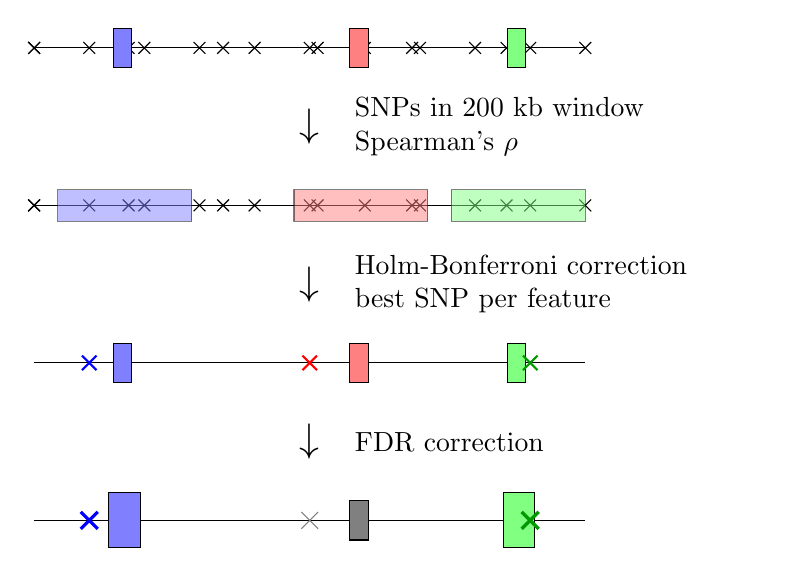
\begin{tikzpicture}
    [feature/.style={rectangle, draw, minimum height=5mm},
     cross/.style={cross out, draw, minimum size=2*(#1-\pgflinewidth), 
     inner sep=0pt, outer sep=0pt},
     cross/.default={1.2mm}]
    \coordinate (5prime);
    \coordinate [right=7cm of 5prime] (3prime);
    \draw (5prime) -- (3prime);
    \draw [decorate, decoration={crosses, segment length=7mm, shape size=1.5mm}]
          (5prime) -- (3prime);
    \draw [decorate, 
           decoration={crosses, segment length=12mm, shape size=1.5mm}] 
          (5prime) -- (3prime);
    \node [feature, right=1cm of 5prime, fill=blue!50!white] (f1) { };
    \node [feature, right=4cm of 5prime, fill=red!50!white] (f2) { };
    \node [feature, right=6cm of 5prime, fill=green!50!white] (f3) { };

    \uncover<2->{

    \coordinate [below=2cm of 5prime] (5prime2);
    \coordinate [below=2cm of 3prime] (3prime2);
    \draw (5prime2) -- (3prime2);
    \draw [decorate, decoration={crosses, segment length=7mm, shape size=1.5mm}]
          (5prime2) -- (3prime2);
    \draw [decorate, 
           decoration={crosses, segment length=12mm, shape size=1.5mm}] 
          (5prime2) -- (3prime2);
    \draw [fill=blue!50!white, opacity=0.5] ($(5prime2) + (0.3cm, 0.2cm)$) 
          rectangle ($(5prime2) + (2cm, -0.2cm)$);
    \draw [fill=red!50!white, opacity=0.5] ($(5prime2) + (3.3cm, 0.2cm)$) 
          rectangle ($(5prime2) + (5cm, -0.2cm)$);
    \draw [fill=green!50!white, opacity=0.5] ($(5prime2) + (5.3cm, 0.2cm)$) 
          rectangle ($(5prime2) + (7cm, -0.2cm)$);
    \path (5prime) -- node (mid1) {\Large{$\downarrow$}} (3prime2);
    \node [right=2mm of mid1, text width=5cm] {SNPs in 200 kb window \\
    Spearman's $\rho$};

    }\uncover<3->{

    \coordinate [below=2cm of 5prime2] (5prime3);
    \coordinate [below=2cm of 3prime2] (3prime3);
    \draw (5prime3) -- (3prime3);
    \node [feature, right=1cm of 5prime3, fill=blue!50!white] (f1) { };
    \node [feature, right=4cm of 5prime3, fill=red!50!white] (f2) { };
    \node [feature, right=6cm of 5prime3, fill=green!50!white] (f3) { };
    \node [cross, blue, thick] at ($(5prime3) + (7mm, 0mm)$) { };
    \node [cross, red, thick] at ($(5prime3) + (35mm, 0mm)$) { };
    \node [cross, green!60!black, thick] at ($(5prime3) + (63mm, 0mm)$) { };
    \path (5prime2) -- node (mid2) {\Large{$\downarrow$}} (3prime3);
    \node [right=2mm of mid2, text width=5cm] {Holm-Bonferroni correction \\ best SNP per feature};

    }\uncover<4->{

    \coordinate [below=2cm of 5prime3] (5prime4);
    \coordinate [below=2cm of 3prime3] (3prime4);
    \draw (5prime4) -- (3prime4);
    \node [feature, minimum height=7mm, minimum width=4mm, right=1.15cm of
    5prime4, anchor=center, fill=blue!50!white] (f1) { };
    \node [feature, right=4cm of 5prime4, fill=gray] (f2) { };
    \node [feature, right=5.95cm of 5prime4, minimum height=7mm, minimum width=4mm, fill=green!50!white] (f3) { };
    \node [cross, cross=1.5mm, blue, very thick] at ($(5prime4) + (7mm, 0mm)$) { };
    \node [cross, gray] at ($(5prime4) + (35mm, 0mm)$) { };
    \node [cross, cross=1.5mm, green!60!black, very thick] at ($(5prime4) + (63mm, 0mm)$) { };
    \path (5prime3) -- node (mid3) {\Large{$\downarrow$}} (3prime4);
    \node [right=2mm of mid3] {FDR correction};

    }
\end{tikzpicture}

        \tikzexternalenable
    \end{center}
\end{frame}

\begin{frame}{Removing Principal Components}
    \begin{columns}
    \begin{column}{0.4\textwidth}
        \begin{itemize}
            \item technical, environmental, and biological covariates can swamp
                out QTL effects
            \uncover<2->{
            \item correct by removing principal components 
            }\uncover<3->{
            \item number of peaks with a QTL plateaus at 10 PCs, while genes and
                CpGs continue to increase
            }\uncover<4->{
            \item for this analysis, removed 10 PCs from all data
            }
        \end{itemize}
    \end{column}
    \begin{column}{0.6\textwidth}
        ../../plots/qtl_pca.tex
    \end{column}
    \end{columns}
\end{frame}

\begin{frame}{Identifying multi-QTLs}
\begin{columns}
    \begin{column}{0.5\textwidth}
        \begin{itemize}
            \item By intersecting QTL sets, found 240 gene, CpG, and peak
                triples which shared the same QTL 
        \end{itemize}
        ../../plots/qtl_venn.tex
    \end{column}
    \pause
    \begin{column}{0.5\textwidth}
        \begin{itemize}
            \item Also assessed QTL overlap using $\pi_0$ approach 
        \end{itemize}
        \vspace{-0.3cm}
        % Created by tikzDevice version 0.7.0 on 2015-04-05 15:43:56
% !TEX encoding = UTF-8 Unicode
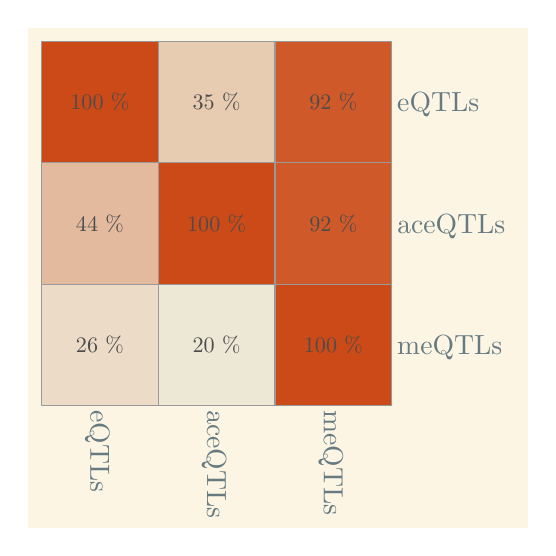
\begin{tikzpicture}[x=1pt,y=1pt]
\definecolor[named]{fillColor}{rgb}{0.99,0.96,0.89}
\path[use as bounding box,fill=fillColor] (0,0) rectangle (180.67,180.67);
\begin{scope}
\path[clip] (  0.00,  0.00) rectangle (180.67,180.67);
\definecolor[named]{drawColor}{rgb}{0.60,0.60,0.60}
\definecolor[named]{fillColor}{rgb}{0.80,0.29,0.09}

\path[draw=drawColor,line width= 0.4pt,line join=round,line cap=round,fill=fillColor] (  5.02,131.80) rectangle ( 47.20,175.66);
\definecolor[named]{fillColor}{rgb}{0.89,0.73,0.62}

\path[draw=drawColor,line width= 0.4pt,line join=round,line cap=round,fill=fillColor] (  5.02, 87.95) rectangle ( 47.20,131.80);
\definecolor[named]{fillColor}{rgb}{0.92,0.86,0.78}

\path[draw=drawColor,line width= 0.4pt,line join=round,line cap=round,fill=fillColor] (  5.02, 44.09) rectangle ( 47.20, 87.95);
\definecolor[named]{drawColor}{rgb}{0.30,0.30,0.30}

\node[text=drawColor,anchor=base,inner sep=0pt, outer sep=0pt, scale=  0.80] at ( 26.11,150.97) {100 \%};

\node[text=drawColor,anchor=base,inner sep=0pt, outer sep=0pt, scale=  0.80] at ( 26.11,107.12) {44 \%};

\node[text=drawColor,anchor=base,inner sep=0pt, outer sep=0pt, scale=  0.80] at ( 26.11, 63.26) {26 \%};
\definecolor[named]{drawColor}{rgb}{0.60,0.60,0.60}
\definecolor[named]{fillColor}{rgb}{0.91,0.80,0.70}

\path[draw=drawColor,line width= 0.4pt,line join=round,line cap=round,fill=fillColor] ( 47.20,131.80) rectangle ( 89.38,175.66);
\definecolor[named]{fillColor}{rgb}{0.80,0.29,0.09}

\path[draw=drawColor,line width= 0.4pt,line join=round,line cap=round,fill=fillColor] ( 47.20, 87.95) rectangle ( 89.38,131.80);
\definecolor[named]{fillColor}{rgb}{0.93,0.91,0.84}

\path[draw=drawColor,line width= 0.4pt,line join=round,line cap=round,fill=fillColor] ( 47.20, 44.09) rectangle ( 89.38, 87.95);
\definecolor[named]{drawColor}{rgb}{0.30,0.30,0.30}

\node[text=drawColor,anchor=base,inner sep=0pt, outer sep=0pt, scale=  0.80] at ( 68.29,150.97) {35 \%};

\node[text=drawColor,anchor=base,inner sep=0pt, outer sep=0pt, scale=  0.80] at ( 68.29,107.12) {100 \%};

\node[text=drawColor,anchor=base,inner sep=0pt, outer sep=0pt, scale=  0.80] at ( 68.29, 63.26) {20 \%};
\definecolor[named]{drawColor}{rgb}{0.60,0.60,0.60}
\definecolor[named]{fillColor}{rgb}{0.81,0.35,0.16}

\path[draw=drawColor,line width= 0.4pt,line join=round,line cap=round,fill=fillColor] ( 89.38,131.80) rectangle (131.56,175.66);

\path[draw=drawColor,line width= 0.4pt,line join=round,line cap=round,fill=fillColor] ( 89.38, 87.95) rectangle (131.56,131.80);
\definecolor[named]{fillColor}{rgb}{0.80,0.29,0.09}

\path[draw=drawColor,line width= 0.4pt,line join=round,line cap=round,fill=fillColor] ( 89.38, 44.09) rectangle (131.56, 87.95);
\definecolor[named]{drawColor}{rgb}{0.30,0.30,0.30}

\node[text=drawColor,anchor=base,inner sep=0pt, outer sep=0pt, scale=  0.80] at (110.47,150.97) {92 \%};

\node[text=drawColor,anchor=base,inner sep=0pt, outer sep=0pt, scale=  0.80] at (110.47,107.12) {92 \%};

\node[text=drawColor,anchor=base,inner sep=0pt, outer sep=0pt, scale=  0.80] at (110.47, 63.26) {100 \%};
\end{scope}
\begin{scope}
\path[clip] (  0.00,  0.00) rectangle (180.67,180.67);
\definecolor[named]{drawColor}{rgb}{0.40,0.48,0.51}

\node[text=drawColor,rotate=270.00,anchor=base west,inner sep=0pt, outer sep=0pt, scale=  1.00] at ( 22.67, 42.33) {eQTLs};

\node[text=drawColor,rotate=270.00,anchor=base west,inner sep=0pt, outer sep=0pt, scale=  1.00] at ( 64.85, 42.33) {aceQTLs};

\node[text=drawColor,rotate=270.00,anchor=base west,inner sep=0pt, outer sep=0pt, scale=  1.00] at (107.03, 42.33) {meQTLs};
\end{scope}
\begin{scope}
\path[clip] (  0.00,  0.00) rectangle (180.67,180.67);
\definecolor[named]{drawColor}{rgb}{0.40,0.48,0.51}

\node[text=drawColor,anchor=base west,inner sep=0pt, outer sep=0pt, scale=  1.00] at (133.53,150.29) {eQTLs};

\node[text=drawColor,anchor=base west,inner sep=0pt, outer sep=0pt, scale=  1.00] at (133.53,106.43) {aceQTLs};

\node[text=drawColor,anchor=base west,inner sep=0pt, outer sep=0pt, scale=  1.00] at (133.53, 62.58) {meQTLs};
\end{scope}
\end{tikzpicture}

        \vspace{-0.5cm}
    \end{column}
\end{columns}
\end{frame}

\tikzexternaldisable
\begin{frame}{Bayesian networks}
    \begin{itemize}
        \item Bayesian networks are directed graphical models, where the
            directed edges represent causal relationships
        \uncover<2-> {
        \item We use conditional Gaussian networks
        }
        \uncover<3-> {
        \item Score = likelihood of data given network
        }
    \end{itemize}
    \begin{center}
        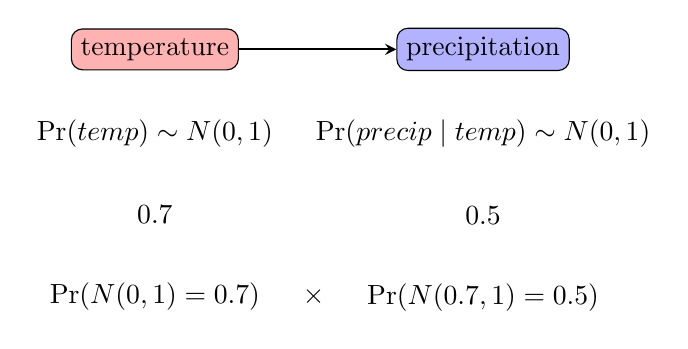
\begin{tikzpicture}
            \node [rectangle, rounded corners, draw, fill=red!30!white] 
            (t) {temperature};
            \node [rectangle, rounded corners, draw, fill=blue!30!white,
            right=2 of t] (p) {precipitation};
            \draw [->, >=stealth, thick] (t) -- (p);

            \uncover<2-> {
            \node [below=0.5 of t] (t1) {$\Pr(\text{temp}) \sim N(0, 1)$};
            \node [below=0.5 of p] (p1) {$\Pr(\text{precip} \mid \text{temp}) \sim N(0, 1)$};
            }

            \uncover<3-> {
            \node [below=0.5 of t1] (t2) {$0.7$};
            \node [below=0.5 of p1] (p2) {$0.5$};
            }

            \uncover<4-> {
            \node [below=0.5 of t2] (t3) {$\Pr(N(0, 1) = 0.7)$};
            \node [below=0.5 of p2] (p3) {$\Pr(N(0.7, 1) = 0.5)$};
            \path (t3) -- node {$\times$} (p3);
            }
        \end{tikzpicture}
    \end{center}
\end{frame}

\begin{frame}{Networks for QTLs}
    \begin{itemize}
        \item \textit{deal} and \textit{CGBayesNets} packages to construct one
            Bayesian network for each multi-QTL by exhaustive search
        \uncover<2->{
        \item With \textit{deal}, edges into genotype were blacklisted
        }\uncover<3->{
        \item Most common network structure was independence
        }\uncover<4->{
        \item Accounted for 42\% of \textit{deal} networks, 29\% of
            \textit{CGBayesNets} networks
        }
    \end{itemize}
    \begin{center}
        %       [g][e|g][ace|g][me|g] 101
%    [g][e|g][ace|e:me][me|g]  14
%      [g][e|g][ace|me][me|g]  13
%       [g][e|g][ace|e][me|g]  12
%      [g][e|me][ace|g][me|g]  12
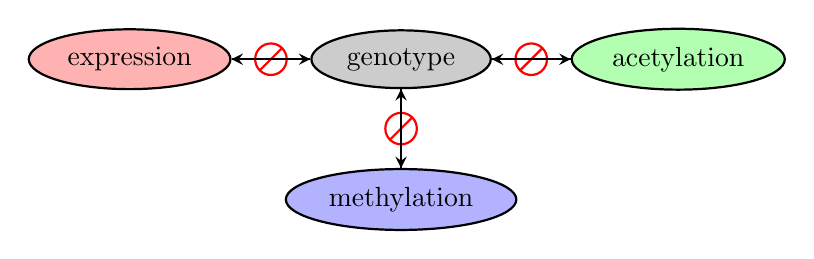
\begin{tikzpicture}
    [every node/.style={ellipse, draw, minimum width=8mm},
     every path/.style={->, >=stealth, thick, draw}]
    \node [fill=black!20!white] (g) {genotype};
    \node [fill=red!30!white, left=of g] (e) {expression};
    \node [fill=green!30!white, right=of g] (a) {acetylation};
    \node [fill=blue!30!white, below =of g] (m) {methylation};

    \uncover<2>{
        \draw (e) -- node [-, draw=red, minimum width=4mm, forbidden sign] { } (g);
        \draw (a) -- node [-, draw=red, minimum width=4mm, forbidden sign] { } (g);
        \draw (m) -- node [-, draw=red, minimum width=4mm, forbidden sign] { } (g);
    }

    \uncover<3->{
        \draw (g) -- (e);
        \draw (g) -- (a);
        \draw (g) -- (m);
    }
\end{tikzpicture}

    \end{center}
\end{frame}
\tikzexternalenable

\begin{frame}{Future Work}
    \begin{itemize}
        \item Expand the number of multi-QTLs
            \begin{itemize}
                \item More that just the best SNP per feature
                \item Identify overlapping QTLs intelligently
            \end{itemize}
        \item More rigourous criterion for number of PCs to remove
        \item Try other packages for network learning (HyPhy)
        \item Are QTLs enriched in SNPs identified in GWAS studies?
        \item Correlations with phenotype (cognitive decline etc.)
    \end{itemize}
\end{frame}

\begin{frame}{Thank you!}
    \begin{columns}
        \begin{column}{0.5\textwidth}
            \small
            \textbf{Harvard / Broad}
            \begin{itemize}
                \setlength\itemsep{-2pt}
                \item Philip L. D. Jager
                \item Lori Chibnik
                \item Jishu Xu
                \item Charles White
                \item Cristin McCabe
                \item Towfique Raj
            \end{itemize}
            \textbf{Rush}
            \begin{itemize}
                \setlength\itemsep{-2pt}
                \item David A Bennett
                \item Chris Gaiteri
                \item Lei Yu
            \end{itemize}
            \textbf{Bioinformatics Training Program}
            \begin{itemize}
                \setlength\itemsep{-2pt}
                \item All the students
                \item Sharon Ruschkowski
            \end{itemize}
        \end{column}
        \normalsize
        \begin{column}{0.5\textwidth}
            \begin{center}
                
\includegraphics[scale=0.3]{logos/cmmt} \\
                \hfill\\
                
\includegraphics[scale=0.2]{logos/bioinfo} \\
                \hfill\\
                
\includegraphics[scale=0.2]{logos/ubc} \\
                \hfill\\
                
\includegraphics[scale=0.1]{logos/nserc} \\
                \hfill\\
                
\includegraphics[scale=0.1]{logos/broad} \\
                \hfill\\
                
\includegraphics[scale=0.1]{logos/rush}
            \end{center}
        \end{column}
    \end{columns}
\end{frame}

\begin{frame}{Software}
    \begin{columns}
    \begin{column}{0.4\textwidth}
    \textbf{QTL analysis}
    \begin{itemize}
        \item
            \href{http://www.bios.unc.edu/research/genomic_software/Matrix_eQTL}
            {Matrix eQTL}
        \item
            \href{http://www.bioconductor.org/packages/release/bioc/html/qvalue.html}
            {qvalue}
    \end{itemize}
    \textbf{Bayesian networks}
    \begin{itemize}
        \item \href{http://cran.r-project.org/web/packages/deal/index.html}
                   {deal}
        \item \href{http://www.cgbayesnets.com}{CGBayesNets}
    \end{itemize}
    \end{column}
    \begin{column}{0.4\textwidth}
    \textbf{Slides}
    \begin{itemize}
        \item \href{http://www.ctan.org/pkg/beamer}{beamer}
        \item \href{https://www.ctan.org/pkg/pgf}{TikZ}
        \item
            \href{http://cran.r-project.org/web/packages/tikzDevice/index.html}
            {tikzDevice}
    \end{itemize}
    \textbf{Plots}
    \begin{itemize}
        \item \href{http://cran.r-project.org/web/packages/pheatmap/index.html}
                   {pheatmap}
        \item \href{http://ggplot2.org/}{ggplot2}
        \item
            \href{http://cran.r-project.org/web/packages/VennDiagram/index.html}
            {VennDiagram}
    \end{itemize}
    \textbf{Colour Scheme}
    \begin{itemize}
        \item \href{http://ethanschoonover.com/solarized}{solarized}
    \end{itemize}
    \end{column}
    \end{columns}
\end{frame}

\end{document}
